\documentclass{article}

% if you need to pass options to natbib, use, e.g.:
%     \PassOptionsToPackage{numbers, compress}{natbib}
% before loading neurips_2020

% ready for submission
% \usepackage{neurips_2020}

% to compile a preprint version, e.g., for submission to arXiv, add add the
% [preprint] option:
%     \usepackage[preprint]{neurips_2020}

% to compile a camera-ready version, add the [final] option, e.g.:
%     \usepackage[final]{neurips_2020}

% to avoid loading the natbib package, add option nonatbib:
     \usepackage[nonatbib]{neurips_2020}


\usepackage[utf8]{inputenc} % allow utf-8 input
\usepackage[T1]{fontenc}    % use 8-bit T1 fonts
\usepackage{hyperref}       % hyperlinks
\usepackage{url}            % simple URL typesetting
\usepackage{booktabs}       % professional-quality tables
\usepackage{amsfonts}       % blackboard math symbols
\usepackage{nicefrac}       % compact symbols for 1/2, etc.
\usepackage{microtype}      % microtypography
\usepackage{amsthm}     % for theorems
\usepackage{algorithm,algorithmic}
\usepackage{mathtools}
\usepackage{amsmath}
\allowdisplaybreaks
\usepackage{amssymb}
\DeclarePairedDelimiter{\norm}{\lVert}{\rVert}
\usepackage{balance}
\usepackage{comment}
\newcommand{\eq}[1]{{Eq~(#1)}}
\newcommand{\figref}[1]{Figure~\ref{#1}}
\newtheorem{theorem}{Theorem}
\newtheorem{thm}{Theorem}
\newtheorem{lemma}[theorem]{Lemma}
\newtheorem{remark}{Remark}
\newcommand{\lkxcom}[1]{{\color{red}{#1}}}

\newcommand{\ov}[1]{{\overline{\mathbf{#1}}}}
%% common packages
\usepackage{amsbsy}
\usepackage{amsmath}
\usepackage{graphicx}
\usepackage{subfigure}
\usepackage{color}
\usepackage{booktabs}

%% to allow citation as footnote
\usepackage{natbib}
% and to reduce footnote font size
\usepackage{etoolbox}
\makeatletter
\patchcmd{\@makefntext}{\insertfootnotetext{#1}}{\insertfootnotetext{\scriptsize#1}}{}{}
\makeatother


%% macros for commenting
\usepackage[normalem]{ulem} % to use \sout
\newcommand{\remove}[1]{{\color{Gray}\sout{#1}}}
\newcommand{\revise}[1]{{\color{blue}#1}}
\newcommand{\commwy}[1]{{\color{red}(wy: #1)}} % Wotao Yin

%% template for beamer

%\mode<presentation>
%{
%  % page number
%  %\setbeamertemplate{footline}{\insertframenumber/\inserttotalframenumber}
%  \setbeamertemplate{footline}[frame number]
%
%  % background and theme
%  \setbeamertemplate{background canvas}[vertical shading][bottom=white!10,top=white!10]
%  \usetheme{default}
%
%  % section in table of contents has numbers
%  \setbeamertemplate{sections/subsections in toc}[sections numbered]
%
%  % no navigation bottoms
%  \setbeamertemplate{navigation symbols}{}
%
%  % itemize, black bullet, %150 spacing between items using "witemize"
%  \setbeamertemplate{itemize items}[circle]
%  \setbeamercolor{itemize item}{fg=black}
%  \setbeamercolor{enumerate item}{fg=black}
%  \setbeamercolor{itemize subitem}{fg=black}
%  \setbeamercolor{enumerate subitem}{fg=black}
%  \newenvironment{witemize}{\itemize\addtolength{\itemsep}{0.0\baselineskip}}{\enditemize}
%
%  % block, black over gray with no shadow
%  \setbeamertemplate{blocks}[rounded][shadow=false]
%  \setbeamercolor{block title}{fg=black,bg=gray!40}
%  \setbeamercolor{block body}{fg=black,bg=gray!10}
%
%  % frametitle, bold, black, centered
%  \setbeamertemplate{frametitle}[default][center]
%  \setbeamercolor{frametitle}{fg=black}
%  \setbeamerfont{frametitle}{shape=\bfseries}
%
%  % line spacing
%  \linespread{1.2}
%
%  \setlength{\parskip}{\smallskipamount}
%}

%% macros for letters

\newcommand{\va}{{\mathbf{a}}}
\newcommand{\vb}{{\mathbf{b}}}
\newcommand{\vc}{{\mathbf{c}}}
\newcommand{\vd}{{\mathbf{d}}}
\newcommand{\ve}{{\mathbf{e}}}
\newcommand{\vf}{{\mathbf{f}}}
\newcommand{\vg}{{\mathbf{g}}}
\newcommand{\vh}{{\mathbf{h}}}
\newcommand{\vi}{{\mathbf{i}}}
\newcommand{\vj}{{\mathbf{j}}}
\newcommand{\vk}{{\mathbf{k}}}
\newcommand{\vl}{{\mathbf{l}}}
\newcommand{\vm}{{\mathbf{m}}}
\newcommand{\vn}{{\mathbf{n}}}
\newcommand{\vo}{{\mathbf{o}}}
\newcommand{\vp}{{\mathbf{p}}}
\newcommand{\vq}{{\mathbf{q}}}
\newcommand{\vr}{{\mathbf{r}}}
\newcommand{\vs}{{\mathbf{s}}}
\newcommand{\vt}{{\mathbf{t}}}
\newcommand{\vu}{{\mathbf{u}}}
\newcommand{\vv}{{\mathbf{v}}}
\newcommand{\vw}{{\mathbf{w}}}
\newcommand{\vx}{{\mathbf{x}}}
\newcommand{\vy}{{\mathbf{y}}}
\newcommand{\vz}{{\mathbf{z}}}

\newcommand{\vA}{{\mathbf{A}}}
\newcommand{\vB}{{\mathbf{B}}}
\newcommand{\vC}{{\mathbf{C}}}
\newcommand{\vD}{{\mathbf{D}}}
\newcommand{\vE}{{\mathbf{E}}}
\newcommand{\vF}{{\mathbf{F}}}
\newcommand{\vG}{{\mathbf{G}}}
\newcommand{\vH}{{\mathbf{H}}}
\newcommand{\vI}{{\mathbf{I}}}
\newcommand{\vJ}{{\mathbf{J}}}
\newcommand{\vK}{{\mathbf{K}}}
\newcommand{\vL}{{\mathbf{L}}}
\newcommand{\vM}{{\mathbf{M}}}
\newcommand{\vN}{{\mathbf{N}}}
\newcommand{\vO}{{\mathbf{O}}}
\newcommand{\vP}{{\mathbf{P}}}
\newcommand{\vQ}{{\mathbf{Q}}}
\newcommand{\vR}{{\mathbf{R}}}
\newcommand{\vS}{{\mathbf{S}}}
\newcommand{\vT}{{\mathbf{T}}}
\newcommand{\vU}{{\mathbf{U}}}
\newcommand{\vV}{{\mathbf{V}}}
\newcommand{\vW}{{\mathbf{W}}}
\newcommand{\vX}{{\mathbf{X}}}
\newcommand{\vY}{{\mathbf{Y}}}
\newcommand{\vZ}{{\mathbf{Z}}}

\newcommand{\cA}{{\mathcal{A}}}
\newcommand{\cB}{{\mathcal{B}}}
\newcommand{\cC}{{\mathcal{C}}}
\newcommand{\cD}{{\mathcal{D}}}
\newcommand{\cE}{{\mathcal{E}}}
\newcommand{\cF}{{\mathcal{F}}}
\newcommand{\cG}{{\mathcal{G}}}
\newcommand{\cH}{{\mathcal{H}}}
\newcommand{\cI}{{\mathcal{I}}}
\newcommand{\cJ}{{\mathcal{J}}}
\newcommand{\cK}{{\mathcal{K}}}
\newcommand{\cL}{{\mathcal{L}}}
\newcommand{\cM}{{\mathcal{M}}}
\newcommand{\cN}{{\mathcal{N}}}
\newcommand{\cO}{{\mathcal{O}}}
\newcommand{\cP}{{\mathcal{P}}}
\newcommand{\cQ}{{\mathcal{Q}}}
\newcommand{\cR}{{\mathcal{R}}}
\newcommand{\cS}{{\mathcal{S}}}
\newcommand{\cT}{{\mathcal{T}}}
\newcommand{\cU}{{\mathcal{U}}}
\newcommand{\cV}{{\mathcal{V}}}
\newcommand{\cW}{{\mathcal{W}}}
\newcommand{\cX}{{\mathcal{X}}}
\newcommand{\cY}{{\mathcal{Y}}}
\newcommand{\cZ}{{\mathcal{Z}}}

\newcommand{\ri}{{\mathrm{i}}}
\newcommand{\rr}{{\mathrm{r}}}


%% macros for math notions and operators

\newcommand{\RR}{\mathbb{R}}
\newcommand{\EE}{\mathbb{E}}
\newcommand{\CC}{\mathbb{C}}
\newcommand{\ZZ}{\mathbb{Z}}
\renewcommand{\SS}{{\mathbb{S}}}
\newcommand{\SSp}{\mathbb{S}_{+}}
\newcommand{\SSpp}{\mathbb{S}_{++}}
\newcommand{\sign}{\mathrm{sign}}
\newcommand{\Sign}{\mathrm{Sign}}
\newcommand{\vzero}{\mathbf{0}}
\newcommand{\vone}{{\mathbf{1}}}
\newcommand{\Null}{{\mathrm{Null}}}
\newcommand{\dist}{{\mathrm{dist}}}
\newcommand{\Co}{{\mathbf{Co}}}

\newcommand{\op}{{\mathrm{op}}} % subscript for operator norm
\newcommand{\opt}{{\mathrm{opt}}} % subscript for optimal solution
\newcommand{\supp}{{\mathrm{supp}}} % support
\newcommand{\Prob}{{\mathrm{Prob}}} % probability
\newcommand{\Diag}{{\mathrm{Diag}}} % vector -> diagonal matrix
\newcommand{\diag}{{\mathrm{diag}}} % matrix diagonal -> vector
\newcommand{\dom}{{\mathrm{dom}}} % domain
\newcommand{\grad}{{\nabla}}    % gradient
\newcommand{\tr}{{\mathrm{tr}}} % trace
\newcommand{\TV}{{\mathrm{TV}}} % total variation
\newcommand{\Proj}{{\mathrm{Proj}}}
\DeclareMathOperator{\shrink}{shrink} % shrinkage
\DeclareMathOperator*{\argmin}{arg\,min}
\DeclareMathOperator*{\argmax}{arg\,max}
\DeclareMathOperator*{\mini}{minimize}
\DeclareMathOperator*{\maxi}{maximize}
\DeclareMathOperator*{\Min}{minimize}
\DeclareMathOperator*{\Max}{maximize}
\newcommand{\prox}{{\mathbf{prox}}}
\newcommand{\st}{{\quad\text{s.t.}~}}

%% macros for environments math equations

\newcommand{\MyFigure}[1]{../fig/#1}

\newcommand{\bc}{\begin{center}}
\newcommand{\ec}{\end{center}}

\newcommand{\bdm}{\begin{displaymath}}
\newcommand{\edm}{\end{displaymath}}

\newcommand{\beq}{\begin{equation}}
\newcommand{\eeq}{\end{equation}}

\newcommand{\bfl}{\begin{flushleft}}
\newcommand{\efl}{\end{flushleft}}

\newcommand{\bt}{\begin{tabbing}}
\newcommand{\et}{\end{tabbing}}

\newcommand{\beqn}{\begin{eqnarray}}
\newcommand{\eeqn}{\end{eqnarray}}

\newcommand{\beqs}{\begin{align*}} % no equation numbers
\newcommand{\eeqs}{\end{align*}}  % no equation numbers

%% macros for theorem-like environments

% \newtheorem{theorem}{Theorem}
% \newtheorem{condition}{Condition}
\newtheorem{assumption}{Assumption}
\newtheorem{definition}{Definition}
% \newtheorem{corollary}{Corollary}
% \newtheorem{remark}{Remark}
% \newtheorem{lemma}{Lemma}
% \newtheorem{proof}{Proof}
% \newtheorem{proof*}{Proof}
% \newtheorem{proposition}{Proposition}
%\newtheorem{example}{Example}

% \newtheorem{example}[remark]{Example}



\newtheorem*{assumption*}{Assumption}

\title{The Blessing of FedAvg's Linear Speedup in Federated Learning}

\author{}

\begin{document}

\maketitle

\begin{abstract}
Federated learning is a distributed learning paradigm that enables learning
a model jointly over a large number of workers without sharing the private
data on local workers. The characteristics of non-identically distributed data
across the network and low device participation brings significant challenges
in analyzing the convergence of federated learning algorithms. Prior works
have either analyzed the convergence with i.i.d. data, or with full device
participation, and often with suboptimal rates. In this work, we provide a
comprehensive analysis of the convergence rate of Federated Averaging (FedAvg)
with SGD and Nesterov SGD updates for general convex problems with arbitrarily
heterogeneous data. Firstly we show that the convergence rates enjoy a linear
speedup in the number of participating workers for all convex smooth problems
for both algorithms.  Furthermore, in the overparamterized setting, we prove that the convergence under FedAvg is in fact exponential, also with a speedup factor linear in the number of workers. We also propose a new accelerated federated learning algorithm that further improves this convergence rate with provable guarantees in the linear regression setting. Empirical evaluation of the algorithms in various settings match our theoretical results.
\end{abstract}

% !TEX ROOT=./main.tex


\section{Introduction}
Federated learning (FL) is a machine learning setting where many clients (e.g. mobile devices or whole organizations) collaboratively train a model under the orchestration of a central server (e.g. service provider), while keeping the training data decentralized~\cite{kairouz2019advances}.
In recent years, FL has swiftly emerged to be an important learning paradigm~\cite{mcmahan2016communication} --one that enjoys widespread success in applications such as personalized recommendation~\cite{chen2018federated}, virtual assistant~\cite{lamautonomy}, keyboard prediction~\cite{47586} to name a few--for at least two reasons: First, the rapid proliferation of smart devices that are equipped with both computing power and data-capturing capabilities provided the infrastructure core for FL. Second, the rising awareness of privacy and the exponential growth of computational power (blessed by Moore's law) in mobile devices have made it increasingly attractive to push the computation to the edge.

Despite its promise and broad applicability in our current era, the potential value FL delivers is coupled with the unique challenges it brings forth. In particular,
when FL learns a single statistical model using data from across all the devices while keeping each individual device's data isolated (and hence private)~\cite{kairouz2019advances}, it faces two challenges that are absent in centralized optimization and traditional distributed optimization~\cite{li2019convergence,smith2017federated}:
\begin{enumerate}
\item\textbf{Statistical heterogeneity:} data distributions in different devices are different.
\item\textbf{System heterogeneity:} only a subset of devices may access the central server at each time. 
\end{enumerate}

% Gaps in the theoretical understanding. 
To address these challenges, Federated Averaging (FedAvg)~\cite{mcmahan2016communication} was proposed as a particularly effective heuristic, which has enjoyed great empirical success~\cite{47586}. This success has since motivated a growing line of research efforts into understanding its theoretical convergence guarantees in various settings. Most existing convergence guarantees of FedAvg were either established in simplified settings~\cite{stich2018local,khaled2019first,wang2018cooperative,yu2019parallel,khaled2020tighter,li2018federated,koloskova2020unified}, have restrictive assumptions~\cite{haddadpour2019convergence} or provide a suboptimal 
convergence rate~\cite{li2019convergence}. Furthermore, the convergence of
FedAvg's accelerated variants~\cite{yu2019linear,huo2020faster,liu2019accelerating} in the general heterogeneous and convex setting is unknown. At the heart of the success of FL is the \emph{linear speedup} property with respect to the number of participating clients that can be achieved with infrequent communications. Although theoretical results of this kind are abundant in distributed and decentralized optimization~\cite{yu2019linear,yu2019parallel,stich2018local,khaled2020tighter,koloskova2020unified}, generalization to the FL setting with both types of heterogeneity is currently lacking.

\subsection{Related Works}
\textbf{Convergence of FedAvg}
There have been a considerable amount of convergence results in distributed stochastic optimization with infrequent communications that establish linear speedup in the number of clients. However, most of these prior works provide
convergence guarantees under simplified settings, where either statistical
heterogeneity~\cite{stich2018local,zhou2017convergence,wang2018cooperative,woodworth2018graph,haddadpour2019convergence} or system
heterogeneity~\cite{yu2019parallel,wang2019adaptive,khaled2019first,jiang2018linear,koloskova2020unified} is not
considered, and the associated algorithm is often referred to as local SGD. ~\cite{li2019convergence} is the first to provide convergence of FedAvg for general strongly convex problems considering both statistical heterogeneity and system heterogeneity, yet it
didn't achieve linear speedup \cite{yu2019parallel,haddadpour2019convergence,stich2018local}. In~\cite{haddadpour2019convergence,liang2019variance,huo2020faster,jiang2018linear}, the convergence of FedAvg for non-convex problems has been studied, whereas this paper focuses on convex settings.
\begin{comment}
However, \cite{huo2020faster} did not discuss the linear speedup and the theorems in \cite{haddadpour2019convergence,liang2019variance} failed to cover the accelerated version of
FedAvg. 
\end{comment}

\textbf{Accelerating Stochastic Federated Learning Algorithms.}
% The accelerated SGD methods has achieved optimal convergence rate in strongly convex
% optimization~\cite{nesterov1983method}.
The convergence of accelerated FL algorithms using momentum (Nesterov and Heavy Ball) updates has been studied mostly in non-convex settings~\cite{yu2019linear,huo2020faster}. \cite{yu2019linear} does not consider system heterogeneity, while the result in \cite{huo2020faster} does not have linear speedup. Furthermore, the rates cannot improve over SGD-based algorithms in general. \cite{liu2019accelerating} provides an acceleration result for FedAvg with accelerated GD. \cite{liang2019variance} considers variance reduction based acceleration of FedAvg. This paper considers accelerated FedAvg with momentum-based stochastic updates in general and overparameterized convex settings.

\begin{comment}
	In this work, we provide a novel accelerated FedAvg with improved convergence rates under a popular overparameterized setting. 
\end{comment}




% Our contributions
% \subsection{Contributions}
\subsection{Our Contributions.}
We provide a comprehensive convergence analysis
of FedAvg and its accelerated variants in the presence of both system and statistical heterogeneity (see Table~\ref{tb:convergencerateintro}).
Our results demonstrate the desirable linear speedup property with respect to the number of participating clients.
More specifically, for strongly convex and smooth problems, we show 
that FedAvg admits a convergence rate of 
{\small{$\cO(1/NT)$}}, and local steps can be as large as {\small{$\cO(\sqrt{T/N})$}}. For convex and smooth objectives, the rate is {\small{$\cO(1/\sqrt{NT})$}}. 
Moreover, we show that FedAvg with Nesterov acceleration also enjoys the same rates and speedup. 
%The same conclusions are equally applied for Nesterov accelerated FedAvg. 
To the best of our knowledge, this is the first linear speedup result for FedAvg and accelerated variants in the fully heterogeneous FL setting. Furthermore, 
we propose a new variant of FedAvg and provide the first improved convergence rate for stochastic momentum-accelerated FedAvg in the popular overparamterized setting.
Last but not least, we systematically examine the convergence rate of
FedAvg and its accelerated variants on both a synthetic dataset and  a real-world dataset. The empirical observations are well-aligned with the obtained theoretical findings.


\begin{table}[h!]
\centering
{\small
\begin{tabular}{|c|c|c|c|}\hline 
	Participation \textbackslash\ Objective function            & Strongly Convex        & Convex  & Overparameterized \\ \hline \hline
	Full                         & $\cO(\frac{1}{NT}+\frac{E^{2}}{T^{2}})$    &  $\mathcal{O}\left(\frac{1}{\sqrt{NT}}+\frac{NE^{2}}{T}\right)$   & $\cO(\exp(-\frac{NT}{E}))$    \\ \hline
	Partial                      &  $\cO\left(\frac{E^{2}}{KT}+\frac{E^{2}}{T^{2}}\right)$   &  $\cO\left(\frac{E^2}{\sqrt{KT}}+\frac{KE^2}{T} \right)$ & $\cO(\exp(-\frac{KT}{E}))$     \\ \hline
\end{tabular}
}
\caption{Our convergence results for FedAvg and accelerated FedAvg in this paper.}
\label{tb:convergencerateintro}
\end{table}

% Our theoretical results not only cover all general convex objectives, including strongly convex cases, convex smooth cases and convex non-smooth cases, but also provide tighter convergence guarantee for all convex smooth objectives, which shows the convergence rate enjoys a linear speedup w.r.t.
% the number of workers.
% Furthermore, we studied a popular over-parameterized setting~\cite{liu2018accelerating} where the optimal solution can obtain zero training loss. In this scenario, we provide a novel accelerated FL algorithm improving
% the convergence rate of FedAvg. Last but not least, we conduct extensive
% evaluation on both synthetic and real-world dataset, which demonstrates that our theoretical indications is well-aligned with the empirical observations.


\textbf{Notations.}
Throughout the paper, we adopt the following notations. Let $N$ be the total
number of local devices, and $K \leq N$ is the maximal number of devices
that are accessible to the central server.  Let $T$ be the total number of stochastic updates performed by each local device, $E$ be the local steps between two consecutive server communications. Thus, $T/E$ is
the number of communications.

% \textbf{Organization} 
% The reminader of this paper is organized as follows. In Section 




% Intro and related work.
% sec 4. linear speedup of FedAvg,  sec 5. linear speedup of Accelerated FedAvg.
% sec 6 linear regression in 
% 1. this is the first result on the exponential convergence of FedAvg algorithms in the
% interpolation setting with linear speedup in the number of workers and explicit dependence on the
% communication interval E.  
% 2. Improved convergence rate over FedAvg for For the overparamterized quadratic problem. 

% without considering statistical heterogeneity
% or system heterogeneity~\cite{stich2018local,khaled2019first,wang2018cooperative,yu2019parallel,yu2019linear} or suboptimal 
% convergence rate~\cite{li2019convergence}.

% is perhaps the most widely adopted optimization algorithm, which runs local
% Stochastic Gradient Descent (SGD) updates on a subset of devices
% and synchronize the local models once in a while. 
% The empirical success of FedAvg and its variants have
% attracted lots of efforts~\cite{li2018federated,stich2018local,khaled2019first,yu2019parallel,haddadpour2019convergence,li2019convergence,huo2020faster} on analyzing its convergence properties. 
% There are few key challenges that differentiates the theoretical analysis
% of FL from the tradition distribution optimization: 
% 1) The data is non-identically distributed across the workers, which means the
% data in each local device cannot be regarded as samples drawn from
% a same distribution. 
% 2) The workers are not active at every communication
% round. In FL, the central server has no control over the local devices. 
% It is more practical to assume only a subset of workers is active during
% each communication round. 

% The current gaps in FL.
% However, most of prior works~\cite{li2018federated,stich2018local,khaled2019first,yu2019parallel,haddadpour2019convergence} either assume
% the data is identically distributed or the all devices are active, which
% violates the practical characteristic in FL. The most recent work~\cite{li2019convergence} firstly presents $O(1/T)$ convergence guarantee without 
% making those unrealistic assumptions while their analysis focused 
% on strongly convex case only and the relation between the number of active
% workers and the convergence rate is not clearly discussed. 


% !TEX ROOT=./main.tex


\section{Problem Setting}

\begin{align}
	\min _{\mathbf{w}}\left\{F(\mathbf{w}) \triangleq \sum_{k=1}^{N} p_{k} F_{k}(\mathbf{w})\right\}
	\label{eq:problem}
\end{align}
where $N$ is the number of devices, and $p_k$ is the weight of the k-th device
such that $p_k \geq 0$ and $\sum_{k=1}^N p_k = 1$. Suppose the k-th device
holds the nk training data: $x_{k,1}, x_{k,2}, \dots, x_{k,n_k}$ . The local
$k \in S_t^K$ objective $F_k(\cdot)$ is defined by

\begin{align}
F_{k}(\mathbf{w}) \triangleq \frac{1}{n_{k}} \sum_{j=1}^{n_{k}} \ell\left(\mathbf{w} ; x_{k, j}\right)	
\label{eq:localloss}
\end{align}

% The summary of all assumptions:

% \begin{assumption}
% $F_{1}, \cdots, F_{N}$ are all $L$-smooth: for all  $\mathbf{v}$  and $\mathbf{w}$, $F_{k}(\mathbf{v}) \leq F_{k}(\mathbf{w})+(\mathbf{v}- \\ \mathbf{w})^{T} \nabla F_{k}(\mathbf{w})+\frac{L}{2}\|\mathbf{v}-\mathbf{w}\|_{2}^{2}$.
% \end{assumption}

% \begin{assumption}
% $F_1,\dots, F_N$ are all convex: for all $\vv$ and $\vw$, 
% $F_k(\vv) \geq F_k(\vw)+(\vv -\vw)^T \grad F_k(\vw)$. \label{ass:cvx}
% \end{assumption}
% \begin{assumption}
% $	F_{1}, \cdots, F_{N} \text { are all } \mu \text { -strongly convex: for all v and } \mathbf{w}, F_{k}(\mathbf{v}) \geq F_{k}(\mathbf{w})+(\mathbf{v}- \\ \mathbf{w})^{T} \nabla F_{k}(\mathbf{w})+\frac{\mu}{2}\|\mathbf{v}-\mathbf{w}\|_{2}^{2}$
% \end{assumption}

% \begin{assumption}
% Let $\xi_{t}^{k}$ be sampled from the k-th device's local data uniformly at random. The variance of stochastic gradients in each device is bounded:
% $\mathbb{E}\left\|\nabla F_{k}\left(\mathbf{w}_{t}^{k}, \xi_{t}^{k}\right)-\nabla F_{k}\left(\mathbf{w}_{t}^{k}\right)\right\|^{2} \leq \sigma_{k}^{2}$, for $k = 1,..., N$.
% \end{assumption}

% \begin{assumption}
% The expected squared norm of stochastic gradients is uniformly bounded. i.e.,
% $\mathbb{E}\left\|\nabla F_{k}\left(\mathbf{w}_{t}^{k}, \xi_{t}^{k}\right)\right\|^{2} \leq G^{2}$, for all $k = 1,..., N$ and $t=0, \dots, T-1$.
% \end{assumption}

\section{Notations}


Let $\vw_t^k$ be the model parameter maintained in the k-th device at the t-th step. $\cI_E$ is a set of global synchronization steps, i.e., $\cI_E = \{n E|n = 1, 2, 3,\dots \}$. If $t+1 \in \cI_E$, which means we communicate the server with (all) clients at time step $t+1$. $\vv^k_{t+1}$ is the immediate result of one step SGD update from $\vw^k_{t}$.
$\xi_{t}^{k}$ denotes the data sampled from k-th device’s local data uniformly at random.
Follow the common practice, we define two virtual sequences $\overline{\mathbf{v}}_{t}$ and $\overline{\mathbf{w}}_{t}$. For full device participation and $t \notin \cI_E$,
$\ov{v}_t = \ov{w}_t =\sum_{k=1}^{N} p_{k} \mathbf{v}_{t}^{k}$. In partial participation, $t \in \cI_E$, $\ov{w}_t \neq \ov{v}_t$ since $\ov{v}_t=\sum_{k=1}^{N} p_{k} \mathbf{v}_{t}^{k}$ while $\sum_{k\in \cS_t}\mathbf{w}_{t}^{k}$. However, we can
set unbiased sampling strategy such that $ \EE_{\cS_t} \ov{w}_t = \ov{v}_t$.
$\overline{\mathbf{v}}_{t+1}$ is one-step SGD from $\overline{\mathbf{w}}_{t}$. 
\begin{align}
\overline{\mathbf{v}}_{t+1}=\overline{\mathbf{w}}_{t}-\eta_{t} \mathbf{g}_{t}	\label{eq:vbar}
\end{align}
% $t+1 \in \cI_E$, we can fetch $\overline{\vw}_{t+1}$, we can communicate $\overline{\vw}_{t+1}$ to all devices.
where $\vg_{t} = \sum_{k=1}^{N} p_{k} \vg_{t,k} $ is one-step stochastic gradient, averaged over all devices. 
\begin{align}
\vg_{t,k} \left\{\begin{array}{ll} 
 = \nabla F_{k}\left(\mathbf{w}_{t}^{k},\xi_{t}^{k} \right)  &  \text{smooth}\\
 \in \partial F_{k}\left(w_{t}^{k}, \xi_{t}^{k}\right)  & \text{non-smooth}
 \end{array}\right.
\end{align}
Similarly, we denote the expected one-step gradient $\ov{g}_{t}= \EE_{\xi_t}[\vg_t] = \sum_{k=1}^{N} p_{k} \EE_{\xi_{t}^{k}} \vg_{t,k}$, where
\begin{align}
\EE_{\xi_{t}^{k}} \vg_{t,k}  \left\{\begin{array}{ll} 
 = \nabla F_{k}\left(\mathbf{w}_{t}^{k}\right)  &  \text{smooth}\\
 \in \partial F_{k}\left(w_{t}^{k}\right)  & \text{non-smooth}
 \end{array}\right.
\end{align}
and we use $\xi_t = \{\xi_t^k\}_{k=1}^N$ denotes samples at all devices at time step $t$. 

The updates of FedAve with partial device activation is given by: 
\begin{align} 
\mathbf{v}_{t+1}^{k} &=\mathbf{w}_{t}^{k}-\eta_{t} \nabla F_{k}\left(\mathbf{w}_{t}^{k}, \xi_{t}^{k}\right) \\ \mathbf{w}_{t+1}^{k} &=\left\{\begin{array}{ll}\mathbf{v}_{t+1}^{k} & \text { if } t+1 \notin \mathcal{I}_{E}, \\ 
\sum_{k \in \cS_{t+1}} \mathbf{v}_{t+1}^{k} & \text { if } t+1 \in \mathcal{I}_{E}\end{array}\right.
\end{align}

In~\cite{li2019convergence}, two types of unbiased sampling strategies are considered in Lemma 5. 
The sampling scheme I establishes $\cS_{t+1}$ by i.i.d. sampling the devices with replacement,
in this case the upper bound of expected square norm of $\ov{w}_{t+1} - \ov{v}_{t+1}$ is given by:
\begin{align}
\EE_{\cS_{t+1}}\left\|\ov{w}_{t+1} - \ov{v}_{t+1}\right\|^2	\leq \frac{4}{K} \eta_t^2 E^2G^2
\end{align}
The sampling scheme II establishes $\cS_{t+1}$ by uniformly sampling all devices without
replacement, in which we have the 
\begin{align}
\EE_{\cS_{t+1}}\left\|\ov{w}_{t+1} - \ov{v}_{t+1}\right\|^2	\leq \frac{4(N - K)}{K(N-1)} \eta_t^2 E^2G^2
\end{align}
We denote this upper bound as follows for concise presentation. 
\begin{align}
	\EE_{\cS_{t+1}}\left\|\ov{w}_{t+1} - \ov{v}_{t+1}\right\|^2 \leq  \eta_t^2 C
	\label{eq:partialsample}
\end{align}


\lkxcom{Questions and next steps}
\begin{itemize}
	\item Consider heterogeneity of data: with strongly convex and smooth, we can use optimality gap. with non-smooth, we can use weighted gradient diversity. 
	\item Nonconvex imply strongly convex: KDD~\cite{zhuo2019federated} has constant learning rate, in our case, we have a diminishing learning rate. 
	\item Quantify biased sampling scheme?
	\item Constant learning rate in other non-strongly convex case. 
\end{itemize}



% !TEX ROOT=./main.tex



\section{Linear Speedup Analysis of FedAvg}
\label{sec:sgd}

In this section, we provide convergence analyses of FedAvg for convex objectives in the general setting with both heterogeneous data (statistical heterogeneity) and partial
participation (system heterogeneity). We show that for strongly convex and smooth objectives,
the convergence of the optimality gap of averaged parameters across
devices is $\mathcal{O}(1/KT)$, while for convex and smooth
objectives, the rate is $\mathcal{O}(1/\sqrt{KT})$. Our results improve upon~\cite{li2019convergence,karimireddy2019scaffold} by showing linear speedup for any number of participating devices, and upon~\cite{khaled2020tighter,koloskova2020unified} by allowing system heterogeneity. The proofs also highlight similarities and distinctions between the strongly convex and convex settings. Detailed proofs are deferred to Appendix Section~\ref{sec:app:fedavg}.

\subsection{Strongly Convex and Smooth Objectives}

We first show that FedAvg has an $\mathcal{O}(1/KT)$ convergence rate
for $\mu$-strongly convex and $L$-smooth objectives. The result relies on a technical improvement over the analysis in~\cite{li2019convergence}. Moreover, it
implies a distinction in communication efficiency that guarantees
this linear speedup for FedAvg with full and partial device participation.
With full participation, $E$ can be chosen as large as $\mathcal{O}(\sqrt{T/N})$
without degrading the linear speedup in the number of workers. On
the other hand, with partial participation, $E$ must be $\mathcal{O}(1)$
to guarantee $\mathcal{O}(1/KT)$ convergence.
\begin{theorem}
	\label{thm:SGD_scvx}Let $\overline{\mathbf{w}}_{T}=\sum_{k=1}^{N}p_{k}\mathbf{w}_{T}^{k}$ in FedAvg,
	$\nu_{\max}=\max_{k}Np_{k}$, and set decaying learning rates $\alpha_{t}=\frac{4}{\mu(\gamma+t)}$
	with $\gamma=\max\{32\kappa,E\}$ and $\kappa=\frac{L}{\mu}$. Then
	under Assumptions~\ref{ass:lsmooth} to \ref{ass:subgrad2} with full device participation, 
	% under Assumptions~\ref{ass:lsmooth},\ref{ass:stroncvx},\ref{ass:boundedvariance},\ref{ass:subgrad2} with full device participation, 
	\begin{align*}
	\mathbb{E}F(\overline{\mathbf{w}}_{T})-F^{\ast}=\mathcal{O}\left(\frac{\kappa\nu_{\max}^{2}\sigma^{2}/\mu}{NT}+\frac{\kappa^{2}E^{2}G^{2}/\mu}{T^{2}}\right),
	\end{align*}
	and with partial device participation with at most $K$ sampled devices
	at each communication round, 
	\begin{align*}
	\mathbb{E}F(\overline{\mathbf{w}}_{T})-F^{\ast}=\mathcal{O}\left(\frac{\kappa E^{2}G^{2}/\mu}{KT}+\frac{\kappa\nu_{\max}^{2}\sigma^{2}/\mu}{NT}+\frac{\kappa^{2}E^{2}G^{2}/\mu}{T^{2}}\right).
	\end{align*}
	\label{th:scvx_sgd}
\end{theorem}
\textbf{Proof sketch.} Because our unified analyses of results in the main text follow the same framework with variations in technical details, we first give an outline of proof  for Theorem~\ref{th:scvx_sgd} to illustrate the main ideas. For full participation, the main ingredient is a recursive contraction bound 
	\begin{align*}
	\mathbb{E}\|\ov{w}_{t+1}-\vw^{\ast}\|^{2} &  \leq(1-\mu\alpha_{t})\mathbb{E}\|\ov{w}_{t}-\vw^{\ast}\|^{2}+\alpha_{t}^{2}\frac{1}{N}\nu_{max}^{2}\sigma^{2}+6\alpha_{t}^{3}LE^{2}G^{2}
	\end{align*}
 where the $\mathcal{O}(\alpha_{t}^{3}E^{2}G^{2})$ term is the key improvement over the bound in~\cite{li2019convergence}, which has $\mathcal{O}(\alpha_{t}^{2}E^2 G^2)$ instead. We then use induction to obtain a non-recursive bound on $\mathbb{E}\|\ov{w}_{T}-\vw^{\ast}\|^{2}$, which is converted to a bound on $\mathbb{E}F(\overline{\mathbf{w}}_{T})-F^{\ast}$ using $L$-smoothness. For partial participation, an additional term $\mathcal{O}(\frac{1}{K} \alpha_t^2 E^2G^2)$ of leading order resulting from sampling variance is added to the contraction bound. To facilitate the understanding of our analysis, please refer to a high-level summary in Appendix~\ref{sec:app:sum}.

\begin{comment}
A crucial ingredient in the proof of Theorem~\ref{th:scvx_sgd} is a one step contraction bound 
	\begin{align*}
	\mathbb{E}\|\ov{w}_{t+1}-\vw^{\ast}\|^{2} & \leq(1-\mu\alpha_{t})\mathbb{E}\|\ov{w}_{t}-\vw^{\ast}\|^{2}+\alpha_{t}^{2}\frac{1}{N}\nu_{max}^{2}\sigma^{2}+6E^{2}L\alpha_{t}^{3}G^{2} 
	\end{align*}
that improves upon the analysis in~\cite{li2019convergence} to deliver the linear speedup. Moreover, analogues of this bound appear in the analyses of the convex setting as well as the Nesterov accelerated FedAvg.\\
\end{comment}

\textbf{Linear speedup. }We compare our bound with that in \cite{li2019convergence},
which is $\mathcal{O}(\frac{1}{NT}+\frac{E^{2}}{KT}+\frac{E^{2}G^{2}}{T})$.
Because the term $\frac{E^{2}G^{2}}{T}$ is also $\mathcal{O}(1/T)$
without a dependence on $N$, for any choice of $E$ their bound cannot
achieve linear speedup. The improvement of our bound comes from the
term $\frac{\kappa^{2}E^{2}G^{2}/\mu}{T^{2}}$, which now is $\mathcal{O}(E^{2}/T^{2})$ and so is not of leading order. As a result, all leading terms scale with $1/N$ in the full device
participation setting, and with $1/K$ in the partial participation
setting. This implies that in both settings, there is a \emph{linear
	speedup} in the number of active workers during a communication
round. We also emphasize that the reason one cannot recover the full participation bound by setting $K=N$ in the partial participation bound is due to the variance generated by sampling. \\
% To our knowledge, this is the first result that explicitly demonstrates
% linear speedup in the number of active workers in the setting with
% both non i.i.d. data and partial participation. \\
\textbf{Communication Complexity.} Our bound implies a distinction
in the choice of $E$ between the full and partial participation settings.
{\color{red}With full participation, the term involving $E$, $\mathcal{O}(E^{2}/T^{2})$, is not of leading order $\mathcal{O}(1/T)$, so we can increase $E$ and reduce the number of communication rounds without degrading the linear speedup in iteration complexity $\mathcal{O}(1/NT)$, as long as $E=\mathcal{O}(\sqrt{T/N})$, since then $\mathcal{O}(E^{2}/T^{2})=\mathcal{O}(1/NT)$
matches the leading term. This corresponds to a communication complexity
of $T/E=\mathcal{O}(\sqrt{NT})$.} In contrast, the bound in \cite{li2019convergence}
does not allow $E$ to scale with $\sqrt{T}$ to preserve $\mathcal{O}(1/T)$
rate, even for full participation. On the other hand, with partial
participation, $\frac{\kappa E^{2}G^{2}/\mu}{KT}$ is also a leading
term, and so $E$ must be $\mathcal{O}(1)$. In this case, our bound
still yields a linear speedup in $K$, which is also confirmed by
experiments. {\color{red}The requirement that $E=\mathcal{O}(1)$ in order to achieve linear speedup in partial participation cannot be removed for our sampling schemes, as the term $\frac{\kappa E^{2}G^{2}/\mu}{KT}$ comes from variance in the sampling process, which is $\mathcal{O}(E^{2}/T^{2})$. In Proposition~\ref{prop:tight} in Section~\ref{sec:app:fedavg} of the appendix, we provide a problem instance where the dependence of the sampling variance on $E$ is tight.}  \\
\textbf{Comparison with related works.} To better understand the significance of the obtained bound, we compare our rates to the best-known results in related settings. \cite{haddadpour2019convergence} proves a linear speedup $\mathcal{O}(1/KT)$ result for strongly convex and smooth objectives\footnote{Their result applies to a larger class of non-convex objectives that satisfy the Polyak-Lojasiewicz condition.}, with $\mathcal{O}(K^{1/3}T^{2/3})$ communication complexity with non-\emph{i.i.d.} data and partial participation. However, their results build on the bounded gradient diversity assumption, which implies the existence of $\mathbf{w}^*$ that minimizes all local objectives (see discussions in Section~\ref{sec:assumptions} and Appendix~\ref{sec:app:comparison}), effectively removing statistical heterogeneity. The bound in \cite{koloskova2020unified} matches our bound in the full participation case, but their framework excludes partial participation \cite[Proposition 1]{koloskova2020unified}. The result of~\cite{karimireddy2019scaffold} applies to the full FL setting, but only has linear speedup when $K=\mathcal{O}(N)$, i.e. close to full participation, whereas our result has linear speedup for any number of participating devices. {\color{red}When there is no data heterogeneity, i.e. in the classical distributed optimization paradigm, communication complexity can be further improved, e.g. \cite{woodworth2020local,woodworth2020minibatch}, but such results are not directly comparable to ours since we consider the setting where individual devices have access to different datasets.}

\begin{comment}
	In this overparameterized setting, we prove a geometric convergence rate (see Section~\ref{sec:overparameterized}), 
	thus improving on the rate in \cite{haddadpour2019convergence} with
	better communication complexity. 
\end{comment}

\subsection{Convex Smooth Objectives}
Next we provide linear speedup analysis of FedAvg with convex and
smooth objectives and show that the optimality gap is $\mathcal{O}(1/\sqrt{KT})$. 
This result complements the strongly convex case in the previous part, as well as the non-convex
smooth setting in \cite{jiang2018linear,yu2019parallel,haddadpour2019convergence},
where $\mathcal{O}(1/\sqrt{KT})$ results are given in terms of averaged
gradient norm, and it also extends the result in~\cite{khaled2020tighter}, which has linear speedup in the convex setting, but only for full participation.
\begin{theorem}
	\label{thm:SGD_cvx}Under Assumptions~\ref{ass:lsmooth},\ref{ass:boundedvariance},\ref{ass:subgrad2} and constant learning
	rate $\alpha_{t}=\mathcal{O}(\sqrt{\frac{N}{T}})$, FedAvg satisfies
	\begin{align*}
	\min_{t\leq T}F(\overline{\mathbf{w}}_{t})-F(\mathbf{w}^{\ast}) & =\mathcal{O}\left(\frac{\nu_{\max}^{2}\sigma^{2}}{\sqrt{NT}}+\frac{NE^{2}LG^{2}}{T}\right)
	\end{align*}
	with full participation, and with partial device participation with $K$ sampled devices at
	each communication round and learning rate $\alpha_{t}=\mathcal{O}(\sqrt{\frac{K}{T}})$,
	\begin{align*}
	\min_{t\leq T}F(\overline{\mathbf{w}}_{t})-F(\mathbf{w}^{\ast}) & =\mathcal{O}\left(\frac{\nu_{\max}^{2}\sigma^{2}}{\sqrt{KT}}+\frac{E^{2}G^{2}}{\sqrt{KT}}+\frac{KE^{2}LG^{2}}{T}\right).
	\end{align*}
\end{theorem}
The analysis again relies on a recursive bound, but without contraction: 
\begin{align*}
	\mathbb{E}\|\ov{w}_{t+1}-\vw^{\ast}\|^{2}+\alpha_{t}(F(\ov{w}_{t})-F(\vw^{\ast})) & \leq \mathbb{E}\|\ov{w}_{t}-\vw^{\ast}\|^{2}+\alpha_{t}^{2}\frac{1}{N}\nu_{\max}^{2}\sigma^{2}+6\alpha_{t}^{3}E^{2}LG^{2}
	\end{align*}
which is then summed over time steps to give the desired bound, with $\alpha_{t}=\mathcal{O}(\sqrt{\frac{N}{T}})$. \\
%
\textbf{Choice of $E$ and linear speedup. }With full participation,
as long as $E=\mathcal{O}(T^{1/4}/N^{3/4})$, the convergence
rate is $\mathcal{O}(1/\sqrt{NT})$ with $\mathcal{O}(N^{3/4}T^{3/4})$
communication rounds. In the partial participation setting, $E$ must
be $O(1)$ in order to achieve linear speedup of $\mathcal{O}(1/\sqrt{KT})$. This is again due to the fact that the sampling variance $\mathbb{E}\|\ov{w}_t-\ov{v}_t\|^2=\mathcal{O}(\alpha_t^2 E^2G^2)$ cannot be made independent of $E$, as illustrated by Proposition \ref{prop:tight}. See also the proof in Section \ref{sec:app:fedavg} for how the sampling variance and the term $E^2G^2/\sqrt{KT}$ are related.  Our result again demonstrates the difference in communication complexities
between full and partial participation, and is to our knowledge the
first result on linear speedup in the general federated learning setting
with both heterogeneous data and partial participation for convex objectives.
\begin{comment}
\textbf{Learning rate. }The learning rate now depends on the final
horizon $T$ of the convergence statement, whereas in the strongly
convex case the learning rate decays as $\mathcal{O}(1/t)$. Such
a requirement $\alpha_{t}=\mathcal{O}(\sqrt{N/T})$ also presents
in \cite{haddadpour2019convergence,yu2019parallel} on non-convex
problems with $\mathcal{O}(1/\sqrt{NT})$ linear speedup convergence results. 
\end{comment}
% !TEX ROOT=./main.tex



\section{Linear Speedup Analysis of Nesterov Accelerated FedAvg}
\label{sec:Nesterov}

A natural extension of the FedAvg algorithm is to use momentum-based
local updates instead of local SGD updates. To our knowledge, the
only convergence analyses of FedAvg with momentum-based stochastic
updates focus on the non-convex smooth case \cite{huo2020faster,yu2019linear,li2018federated}.
In this section, we complete the picture with $\mathcal{O}(1/NT)$
and $\mathcal{O}(1/\sqrt{NT})$ convergence results for Nesterov-accelerated
FedAvg for convex objectives that match the rates from the previous section. Our work the first to provide a unified analysis for FedAvg and Nesterov accelerated FedAvg for convex problems, highlighting the common elements
and distinctions for the two algorithms, whereas previous analysis of momentum accelerated FedAvg algorithms only exist in the non-convex
case (only with full participation)~\cite{yu2019linear} and are scattered and use different notation and proof techniques [16, 17].

As we know from stochastic optimization, Nesterov and other momentum
updates may fail to accelerate over SGD \cite{liu2018accelerating,kidambi2018insufficiency,liu2018toward,yuan2016influence}.
Therefore in Section~\ref{sec:overparameterized} we will specialize to overparameterized
problems where we demonstrate that a particular FedAvg variant with
momentum updates is able to accelerate over the original FedAvg algorithm. 
Detailed proofs of convergence results in this section are deferred to Appendix Section~\ref{sec:app:Nesterovfedavg}.

\subsection{Strongly Convex and Smooth Objectives}
\begin{comment}
We first show that the Nesterov accelerated FedAvg has $\mathcal{O}(1/NT)$
convergence rate for $\mu$-strongly convex and $L$-smooth objectives.
\end{comment}
The Nesterov Accelerated FedAvg algorithm follows the updates:
\begin{align*}
\mathbf{v}_{t+1}^{k} & =\mathbf{w}_{t}^{k}-\alpha_{t}\mathbf{g}_{t,k},\\
\mathbf{w}_{t+1}^{k} & =\begin{cases}
\mathbf{v}_{t+1}^{k}+\beta_{t}(\mathbf{v}_{t+1}^{k}-\mathbf{v}_{t}^{k}) & \text{if }t+1\notin\mathcal{I}_{E},\\
\sum_{k \in \cS_{t+1}}\left[\mathbf{v}_{t+1}^{k}+\beta_{t}(\mathbf{v}_{t+1}^{k}-\mathbf{v}_{t}^{k})\right] & \text{if }t+1\in\mathcal{I}_{E},
\end{cases}
\end{align*}
where $\mathbf{g}_{t,k}:=\nabla F_{k}(\mathbf{w}_{t}^{k},\xi_{t}^{k})$ is
the stochastic gradient sampled on the $k$-th device at time $t$.  
\begin{theorem}
	\label{thm:nesterov_scvx}Let $\overline{\mathbf{v}}_{T}=\sum_{k=1}^{N}p_{k}\mathbf{v}_{T}^{k}$
	and set learning rates $\alpha_{t}=\frac{6}{\mu}\frac{1}{t+\gamma}$,  $\beta_{t-1}=\frac{3}{14(t+\gamma)(1-\frac{6}{t+\gamma})\max\{\mu,1\}}$. Then under Assumptions~\ref{ass:lsmooth},\ref{ass:stroncvx},\ref{ass:boundedvariance},\ref{ass:subgrad2} with full device participation, 
	\begin{align*}
	\mathbb{E}F(\overline{\mathbf{v}}_{T})-F^{\ast}=\mathcal{O}\left(\frac{\kappa\nu_{\max}^{2}\sigma^{2}/\mu}{NT}+\frac{\kappa^{2}E^{2}G^{2}/\mu}{T^{2}}\right),
	\end{align*}
	and with partial device participation with $K$ sampled devices at
	each communication round, 
	\begin{align*}
	\mathbb{E}F(\overline{\mathbf{v}}_{T})-F^{\ast}=\mathcal{O}\left(\frac{\kappa\nu_{\max}^{2}\sigma^{2}/\mu}{NT}+\frac{\kappa E^{2}G^{2}/\mu}{KT}+\frac{\kappa^{2}E^{2}G^{2}/\mu}{T^{2}}\right).
	\end{align*}
\end{theorem}
%
To our knowledge, this is the first convergence result for Nesterov
accelerated FedAvg in the strongly convex and smooth setting. The
same discussion about linear speedup of FedAvg applies to the Nesterov
accelerated variant. In particular, to achieve $\mathcal{O}(1/NT)$
linear speedup, $T$ iterations of the algorithm require only $\mathcal{O}(\sqrt{NT})$
communication rounds with full participation. 


\subsection{Convex Smooth Objectives}

We now show that the optimality gap of Nesterov Accelerated FedAvg has $\mathcal{O}(1/\sqrt{NT})$ rate. This result complements the strongly convex case in the previous
part, as well as the non-convex smooth setting in \cite{huo2020faster,yu2019linear,li2018federated},
where a similar $\mathcal{O}(1/\sqrt{NT})$ rate is given in terms
of averaged gradient norm. 
\begin{theorem}
	\label{thm:Nesterov_cvx}Set learning rates $\alpha_{t}=\beta_{t}=\mathcal{O}(\sqrt{\frac{N}{T}})$. Then under Assumptions~\ref{ass:lsmooth},\ref{ass:boundedvariance},\ref{ass:subgrad2} Nesterov accelerated FedAvg with
	full device participation has rate
	\begin{align*}
	\min_{t\leq T}F(\overline{\mathbf{v}}_{t})-F^{\ast} & =\mathcal{O}\left(\frac{\nu_{\max}^{2}\sigma^{2}}{\sqrt{NT}}+\frac{NE^{2}LG^{2}}{T}\right),
	\end{align*}
	and with partial device participation with $K$ sampled devices at
	each communication round, 
	\begin{align*}
	\min_{t\leq T}F(\overline{\mathbf{v}}_{t})-F^{\ast} & =\mathcal{O}\left(\frac{\nu_{\max}^{2}\sigma^{2}}{\sqrt{KT}}+\frac{E^{2}G^{2}}{\sqrt{KT}}+\frac{KE^{2}LG^{2}}{T}\right).
	\end{align*}
\end{theorem}
%
	It is possible to extend the results in this section to accelerated
    FedAvg algorithms with other momentum-based updates. However, in the
    stochastic optimization setting, none of these methods can achieve a better rate than the original FedAvg with SGD updates for general problems~\cite{kidambi2018insufficiency}.
    For this reason, we will instead turn to the overparameterized setting
    \cite{ma2017power,liu2018accelerating,canziani2016analysis} in the
    next section where we show that FedAvg enjoys geometric convergence
    and it is possible to improve its convergence rate with momentum-based updates.

% !TEX ROOT=./main.tex



\section{Geometric Convergence of FedAvg in the Overparameterized Setting}
\label{sec:overparameterized}
% In this section, we turn to the special setting of overparameterized
% problems, where a non-negative loss function admits a zero-loss global
% minimizer. Such problems are prevalent especially at the age of deep learning,
% where the number of parameters far exceeds the number of data points,
% and perfect fitting is possible. There have been a line of recent
% works showing that SGD and accelerated methods achieve geometric
% convergence in similar settings thanks to the property of \textit{automatic
% variance reduction}~\cite{ma2017power,moulines2011non,needell2014stochastic,schmidt2013fast,strohmer2009randomized}.
% The natural question is whether such a result also holds in the federated
% learning setting. 
% We show that this is indeed the case and establish
% the geometric (linear) convergence of FedAvg with local SGD updates
% with constant step size for general strongly convex and smooth overparameterized
% problems. In addition, we show that the convergence rate speeds up
% linearly in the number of workers $N$ when $N$ is below some problem-dependent
% threshold, while it decreases with $E$ through $1/E$. 
Overparameterization is a prevalent machine learning setting where the
statistical model has much more parameters than the number of training samples
and the existence of parameter choices with zero training loss is
ensured~\cite{allen2018convergence,zhang2016understanding}.  Due to the
property of \textit{automatic variance reduction} in overparameterization,  a
line of recent works proved that SGD and accelerated methods achieve geometric
convergence~\cite{ma2017power,moulines2011non,needell2014stochastic,schmidt2013fast,strohmer2009randomized}.
A natural question is whether such a result still holds in the federated
learning setting. 
In this section, we provide the first geometric convergence rate
of FedAvg for the overparameterized strongly convex and smooth problems,
and show that it preserves linear speedup at the same time.  
We then sharpen this result in the special case of
quadratic problems.
Inspired by recent advances in accelerating SGD~\cite{liu2019accelerating,jain2017accelerating}, 
we further propose a novel momentum-based FedAvg algorithm, which enjoys an
improved convergence rate over FedAvg. Detailed proofs are deferred to Appendix Section~\ref{sec:interpolation}.
\begin{comment}
we deal with the question of whether FedAvg with momentum-based
local updates can outperform FedAvg with SGD updates. In contrast
to the gradient descent setting, Nesterov and Heavy Ball updates are
known to fail to accelerate over SGD, both in the overparameterized
setting and standard convex setting \cite{liu2018accelerating,kidambi2018insufficiency,liu2018toward,yuan2016influence}.
Thus in general one cannot hope to obtain acceleration results for
the FedAvg algorithm with Nesterov and Heavy Ball updates. On the
hopeful side, \cite{jain2017accelerating,liu2018accelerating} introduced
similar algorithms that make modifications of the Nesterov updates
to correct for its ``over-descent''. For quadratic objectives in
the overparamterized setting, \cite{liu2018accelerating} show their
algorithm achieves acceleration over the geometric convergence of
SGD that recovers the well-known $\mathcal{O}(\exp(-t/\sqrt{\kappa})$
acceleration of Nesterov over GD. In the last part, we introduce a
new accelerated FedAvg algorithm by adapting the MaSS algorithm of
\cite{liu2018accelerating} to the federated learning setting. We
show that it achieves geometric convergence for overparameterized
quadratic problems with rate $\mathcal{O}(\exp(-\frac{NT}{E\sqrt{\kappa_{1}\tilde{\kappa}}}))$,
where $\tilde{\kappa}$ is a ``statistical condition number''\cite{liu2018accelerating,jain2017accelerating}
that satisfies $\tilde{\kappa}\leq\kappa_{1}$. Thus our new FedAvg
algorithm achieves a speedup of factor $\sqrt{\kappa_{1}/\tilde{\kappa}}$
over FedAvg with local SGD updates. 
\end{comment}


\subsection{Geometric Convergence of FedAvg in the Overparameterized Setting}
Recall the federated learning problem $\min_{w}\sum_{k=1}^{N}p_{k}F_{k}(\mathbf{w})$
with $F_{k}(\mathbf{w})=\frac{1}{n_{k}}\sum_{j=1}^{n_{k}}\ell(\mathbf{w};\mathbf{x}_{k}^{j})$.
In this section, we consider the standard Empirical Risk Minimization (ERM) setting where $\ell$
is non-negative, $l$-smooth, and convex, and as before, each $F_{k}(\mathbf{w})$ is $L$-smooth and $\mu$-strongly convex. Note that $l\geq L$. This
setup includes many important problems in practice. In the overparameterized
setting, there exists $\mathbf{w}^{\ast}\in\arg\min_{w}\sum_{k=1}^{N}p_{k}F_{k}(\mathbf{w})$
such that $\ell(\mathbf{w}^{\ast};\mathbf{x}_{k}^{j})=0$ for all
$\mathbf{x}_{k}^{j}$. We first show that FedAvg achieves geometric convergence
with linear speedup in the number of workers. 
\begin{theorem}
	\label{thm:overparameterized_general}In the overparameterized setting,
	FedAvg with communication every $E$ iterations
	and constant step size $\overline{\alpha}=\mathcal{O}(\frac{1}{E}\frac{N}{l\nu_{\max}+L(N-\nu_{\min})})$
	has geometric convergence
	\begin{align*}
	\mathbb{E}F(\overline{\mathbf{w}}_{T}) & \leq\frac{L}{2}(1-\overline{\alpha})^{T}\|\mathbf{w}_{0}-\mathbf{w}^{\ast}\|^{2}=\mathcal{O}\left(L\exp(-\frac{\mu}{E}\frac{NT}{l\nu_{\max}+L(N-\nu_{\min})})\cdot\|\mathbf{w}_{0}-\mathbf{w}^{\ast}\|^{2}\right).
	\end{align*}
\end{theorem}
%
\textbf{Linear speedup and Communication Complexity} The linear speedup factor is on the order of $\mathcal{O}(N/E)$ %\frac{N}{E(l\nu_{\max}+L(N-\nu_{\min}))}/\frac{1}{l\nu_{\max}+L(1-\nu_{\min})}\approx\frac{Nl}{E(l+L(N-1))}=
for $N\leq\mathcal{O}(\frac{l}{L})$, i.e. FedAvg with $N$ workers and communication
every $E$ iterations provides a geometric convergence speedup factor
of $\mathcal{O}(N/E)$, for $N\leq\mathcal{O}(\frac{l}{L})$. When $N$ is above
this threshold, however, the speedup is almost constant in the number
of workers. This matches the findings in \cite{ma2017power}. Our
result also illustrates that $E$ can be taken $\mathcal{O}(T^{\beta})$
for any $\beta<1$ to achieve geometric convergence, achieving better communication efficiency than
the standard FL setting. 

\subsection{Overparameterized Quadratic Problems}
We now turn to quadratic problems
and demonstrate how the general bound in Theorem~\ref{thm:overparameterized_general}
can be sharpened to explicitly depend on the condition number of the
system, and how this rate can be further improved with a new FedAvg
algorithm with momentum updates. 

The local device objectives are now given by the sum of squares {\small$F_{k}(\mathbf{w})=\frac{1}{2n_{k}}\sum_{j=1}^{n_{k}}(\mathbf{w}^{T}\mathbf{x}_{k}^{j}-z_{k}^{j})^{2}$},
and there exists $\mathbf{w}^{\ast}$ such that $F(\mathbf{w}^{\ast})\equiv0$.
Define the local Hessian matrix as $H^{k}:=\frac{1}{n_{k}}\sum_{j=1}^{n_{k}}\mathbf{x}_{k}^{j}(\mathbf{x}_{k}^{j})^{T}$, and the stochastic Hessian matrix as $\tilde{H}_{t}^{k}:=\xi_{t}^{k}(\xi_{t}^{k})^{T}$. 
\begin{comment}
In general $H$ has zero eigevalues. However, because the null space
of $H$ and range of $H$ are orthogonal, in our subsequence analysis
it suffices to project $\overline{\mathbf{w}}_{t}-\mathbf{w}^{\ast}$
onto the range of $H$, thus we may restrict to the non-zero eigenvalue
of $H$. We can use $\mathbf{w}^{\ast T}\mathbf{x}_{k}^{j}-z_{k}^{j}\equiv0$
to rewrite the local objectives as $F_{k}(\mathbf{w})=\frac{1}{2}\langle\mathbf{w}-\mathbf{w}^{\ast},H^{k}(\mathbf{w}-\mathbf{w}^{\ast})\rangle\equiv\frac{1}{2}\|\mathbf{w}-\mathbf{w}^{\ast}\|_{H^{k}}^{2}$
so that $F(\mathbf{w})=\frac{1}{2}\|\mathbf{w}-\mathbf{w}^{\ast}\|_{H}^{2}$.
\end{comment}
\begin{comment}
\begin{align*}
F_{k}(w) & =\frac{1}{2n_{k}}\sum_{j=1}^{n_{k}}(w^{T}x_{k,j}-z_{k,j}-(w^{\ast T}x_{k,j}-z_{k,j}))^{2}=\frac{1}{2n_{k}}\sum_{j=1}^{n_{k}}((w-w^{\ast})^{T}x_{k,j})^{2}\\
& =\frac{1}{2}\langle w-w^{\ast},H^{k}(w-w^{\ast})\rangle=\frac{1}{2}\|w-w^{\ast}\|_{H^{k}}^{2}
\end{align*}
\end{comment}
\begin{comment}
Let $\xi_{t}^{k}$ be the stochastic sample on the $k$th device at
time $t$, and define $\tilde{H}_{t}^{k}:=\xi_{t}^{k}(\xi_{t}^{k})^{T}$
as the stochastic Hessian matrix. %	
\end{comment}
\begin{comment}
Note that $\mathbb{E}\tilde{H}_{t}^{k}=\frac{1}{n_{k}}\sum_{j=1}^{n_{k}}\mathbf{x}_{k}^{j}(\mathbf{x}_{k}^{j})^{T}=H^{k}$
and $\mathbf{g}_{t,k}=\nabla F_{k}(\mathbf{w}_{t}^{k},\xi_{t}^{k})=\tilde{H}_{t}^{k}(\mathbf{w}_{t}^{k}-\mathbf{w}^{\ast})$
while $\mathbf{g}_{t}=\sum_{k=1}^{N}p_{k}\nabla F_{k}(\mathbf{w}_{t}^{k},\xi_{t}^{k})=\sum_{k=1}^{N}p_{k}\tilde{H}_{t}^{k}(\mathbf{w}_{t}^{k}-\mathbf{w}^{\ast})$.
\end{comment}
Define $l$ to be the smallest positive number such that $\mathbb{E}\|\xi_{t}^{k}\|^{2}$$\mathbf{\xi}_{t}^{k}$($\mathbf{\xi}_{t}^{k})^{T}\preceq lH^{k}$
for all $k$. Note that $l\leq\max_{k,j}\|\mathbf{x}_{k}^{j}\|^{2}$.
Let $L$ and $\mu$ be lower and upper bounds of non-zero eigenvalues
of $H^{k}$. Define $\kappa_{1}:=l/\mu$ and $\kappa:=L/\mu$. Following
\cite{liu2018accelerating,jain2017accelerating}, we define the statistical
condition number $\tilde{\kappa}$ as the smallest positive real number
such that $\mathbb{E}\left[\langle\xi_{t}^{k}(H^{k})^{-1},\xi_{t}^{k}\rangle\xi_{t}^{k}(\xi_{t}^{k})^{T}\right] \  \preceq\tilde{\kappa}H^{k}$, for all $k$. 
The condition numbers $\kappa_{1}$ and $\tilde{\kappa}$
are important in the characterization of convergence rates for FedAvg
algorithms. Note that $\kappa_{1}>\kappa$ and $\kappa_{1}>\tilde{\kappa}$. 

\subsection{Acceleration of FedAvg with Momentum-based Updates}

We show that the bound in Theorem \ref{thm:overparameterized_general} can be improved to $\mathcal{O}(\exp(-\frac{N}{E\kappa_{1}}t))$ for quadratic problems, then propose a variant of FedAvg that has provable acceleration over FedAvg with SGD updates. 

\begin{theorem}
	\label{thm:overparameterized_quadratic}For the overparamterized quadratic
	problem, FedAvg with communication every $E$
	iterations with constant step size $\overline{\alpha}=\mathcal{O}(\frac{1}{E}\frac{N}{l\nu_{\max}+\mu(N-\nu_{\min})})$
	has geometric convergence:
	\begin{align*}
	\mathbb{E}F(\overline{\mathbf{w}}_{T}) & \leq\mathcal{O}\left(L(1-\frac{N}{E(\nu_{\max}\kappa_{1}+(N-\nu_{\min}))})^{T}\|\mathbf{w}_{0}-\mathbf{w}^{\ast}\|^{2}\right).
	\end{align*}
\end{theorem}

When $N=\mathcal{O}(\kappa_{1})$, the convergence rate is $\mathcal{O}((1-\frac{N}{E\kappa_{1}})^{T})=\mathcal{O}(\exp(-\frac{NT}{E\kappa_{1}}))$,
which exhibits linear speedup in the number of workers, as well as
a $1/\kappa_{1}$ dependence on the condition number $\kappa_{1}$.
Inspired by \cite{liu2018accelerating}, we propose the \textbf{MaSS
	accelerated FedAvg algorithm} (FedMaSS):
\begin{align*}
\mathbf{w}_{t+1}^{k} & =\begin{cases}
\mathbf{u}_{t}^{k}-\eta_{1}^{k}\mathbf{g}_{t,k} & \text{if }t+1\notin\mathcal{I}_{E},\\
\sum_{k=1}^{N}p_{k}\left[\mathbf{u}_{t}^{k}-\eta_{1}^{k}\mathbf{g}_{t,k}\right] & \text{if }t+1\in\mathcal{I}_{E},
\end{cases}\\
\mathbf{u}_{t+1}^{k} & =\mathbf{w}_{t+1}^{k}+\gamma^{k}(\mathbf{w}_{t+1}^{k}-\mathbf{w}_{t}^{k})+\eta_{2}^{k}\mathbf{g}_{t,k}. 
\end{align*}
When $\eta_{2}^{k}\equiv0$, this algorithm reduces to the Nesterov
accelerated FedAvg algorithm. In the next theorem, we demonstrate
that FedMaSS improves the convergence to $\mathcal{O}(\exp(-\frac{NT}{E\sqrt{\kappa_{1}\tilde{\kappa}}}))$.
To our knowledge, this is the first accelerated result of
FedAvg with momentum updates over SGD updates.
\begin{theorem}
	\label{thm:overparameterized_MaSS}For the overparamterized quadratic
	problem, FedMaSS with communication every $E$ iterations and constant
	step sizes $\overline{\eta}_1=\mathcal{O}(\frac{1}{E}\frac{N}{l\nu_{\max}+\mu(N-\nu_{\min})}),\overline{\eta}_{2}=\frac{\overline{\eta}_{1}(1-\frac{1}{\tilde{\kappa}})}{1+\frac{1}{\sqrt{\kappa_{1}\tilde{\kappa}}}},\overline{\gamma}=\frac{1-\frac{1}{\sqrt{\kappa_{1}\tilde{\kappa}}}}{1+\frac{1}{\sqrt{\kappa_{1}\tilde{\kappa}}}}$
	has geometric convergence:
	\begin{align*}
	\mathbb{E}F(\overline{\vw}_{T}) & \leq\mathcal{O}\left((1-\frac{1}{E}\frac{N}{l\nu_{\max}\sqrt{\kappa_{1}\tilde{\kappa}}+(N-\nu_{\min})})^{T}\|w_{0}-w^{\ast}\|^{2}\right).
	\end{align*}
\end{theorem}
\textbf{Speedup of FedMaSS over FedAvg} 
To better understand the significance of the above result, we briefly discuss related works on accelerating SGD.
Nesterov and Heavy Ball updates are known to fail to accelerate over SGD in both the overparameterized
and convex settings~\cite{liu2018accelerating,kidambi2018insufficiency,liu2018toward,yuan2016influence}.
Thus in general one cannot hope to obtain acceleration results for
the FedAvg algorithm with Nesterov and Heavy Ball updates. 
Luckily, recent works in SGD~\cite{jain2017accelerating,liu2018accelerating} introduced
an additional compensation term to the Nesterov updates to address the non-acceleration issue. Surprisingly, 
we show the same approach can effectively improve the rate of FedAvg.
Comparing the convergence rate of FedMass (Theorem~\ref{thm:overparameterized_MaSS}) and FedAvg (Theorem~\ref{thm:overparameterized_quadratic}), when $N=\mathcal{O}(\sqrt{\kappa_{1}\tilde{\kappa}})$,
the convergence rate is $\mathcal{O}((1-\frac{N}{E\sqrt{\kappa_{1}\tilde{\kappa}}})^{T})=\mathcal{O}(\exp(-\frac{NT}{E\sqrt{\kappa_{1}\tilde{\kappa}}}))$
as opposed to $\mathcal{O}(\exp(-\frac{NT}{E\kappa_{1}}))$. Since
$\kappa_{1}\geq\tilde{\kappa}$, this implies a speedup factor of
$\sqrt{\frac{\kappa_{1}}{\tilde{\kappa}}}$ for FedMaSS. On the other
hand, the same linear speedup in the number of workers holds for $N$
in a smaller range of values. 
% !TEX ROOT=./main.tex

\section{Related Works}

% related work on convergence rate
Federated learning (FL) was originally proposed
in~\cite{mcmahan2016communication} for learning a single, global statistal
model from the isolated data stored in a massive number of devices.  The
empirical success of FL~\cite{chen2018federated,47586} has attracted much
attentions on the rigorous theoretical understanding of the leading algorithm 
in the field: Federated Averaging (FedAvg) and its accelerated variants~\cite{liu2019accelerating,haddadpour2019convergence,khaled2019first,li2019convergence,huo2020faster,yu2019linear,yu2019parallel,koloskova2020unified}.

% Non-convex linear speedup
In particular, we focus on the convergence analysis of FedAvg, which
has been discussed in various settings. 
In \cite{yu2019parallel,wang2019adaptive}, the authors provides convergence
rate of FedAvg for non-convex problem, given the data are i.i.d. distributed.
The 







% !TEX ROOT=./main.tex



\section{Numerical Experiments}
\label{sec:exp}

In this section, we empirically examine the theoretical convergence rate of FedAvg on various scenarios, including strongly convex function, convex smooth function, and overparameterized setting, as presented in previous sections.

\textbf{Setup.} Follow the experimental setting in~\cite{stich2018local}, we
conduct experiments on both synthetic datasets and real-world dataset
w8a~\cite{platt1998fast} $(d=300, n=49749)$. We consider the distributed
objectives $F(\vw) = \sum_{k=1}^N p_kF_k(\vw)$, and the objective function on
each local device $k$ includes three cases: 1) \textbf{Strongly convex
objective}: the regularized binary logistic regression problem, $F_k(\vw) =
\frac{1}{N_k} \sum_{i=1}^{N_k} \log( 1+ \exp(-y_i^k \vw^T\vx_i^k) + \lambda
\|\vw\|^2$. The regularization parameter is set to $\lambda = 1/n \approx
1e-5$. 2) \textbf{Convex smooth objective}: the binary logistic regression
problem without regularization. $F_k(\vw) = \frac{1}{N_k} \sum_{i=1}^{N_k}
\log( 1+ \exp(-y_i^k \vw^T\vx_i^k)$. 3) \textbf{Overparameterized setting}:
the linear regression problem without adding noise to the label, $F_k(\vw) =
\frac{1}{N_k} \sum_{i=1}^{N_k} (\vw^T\vx_i^k + b  - y_i^k)^2$.  In the first
two cases, we use the w8a dataset to conduct empirical evaluation. 
In the linear regression problem, we use features from w8a dataset and 
generate a ground truth $w$ to label each instance, which satisfies the
overparameterized setting. For the detailed experimental setup and
hyperparameter setting, please refer to the section~\ref{sec:expsupp} in the
appendix.


% ~\ref{th:strongcvxsmth}~\ref{th:cvxsmoth}~\ref{th:fedmasslr}
\textbf{Linear speedup.} To verify the linear speedup results in Theorems
\lkxcom{cite sgd theorems}, we evaluate the number of iterations needed to reach
$\epsilon$-accuracy in three objectives. We initialize all runs with $\vw_0 = \textbf{0}_d$ and measure. For each configuration, we run three random seeds and report
the best seed results for each configuration $(E, K)$. In each configure, we
extensive search the stepsize from $\min(\eta_0, \frac{nc}{1 + t})$, where
$\eta_0 \in \{0.1, 0.12, 1, 32 \}$ according to different problems and $c$ can
take the values $c = 2^i \ \forall i \in \ZZ$. As the results shown in Figure~\ref{fig:speedup},
the number of iterations to reach the target accuracy $\epsilon$ decreasing 
as the number of workers increase. 

\textbf{The impact of $E$.} We further examine how does the number of epochs 
affect the convergence. As shown in Figure~\ref{fig:e}, the number of iterations
increases as the number of epochs increase, which slow the convergence in
terms of gradient computation. However, it can save communication cost as
the number of rounds decreased when the number of epochs increases.


\textbf{Partial participations.} We verify the linear speedup in the
partial participation settings, where we set $50\%$ of devices
are active. As the results shown in Figure~\ref{fig:partial}, the 
FedAve enjoys linear speedup in various settings even with partial
device participation.

\textbf{Nesterov accelerated FedAvg.} In Figure~\ref{fig:nesterov}, 
report the convergence of Nesterov accelerated FedAvg. The empirical 
observation is aligned with our theorems \lkxcom{cite accelerated theorems} that the acclerated version of FedAvg can also achieve the lienar speedup
w.r.t the number of nodes.

\begin{figure}
\centering
	\begin{tabular}{ccc}
	\hspace{-2em}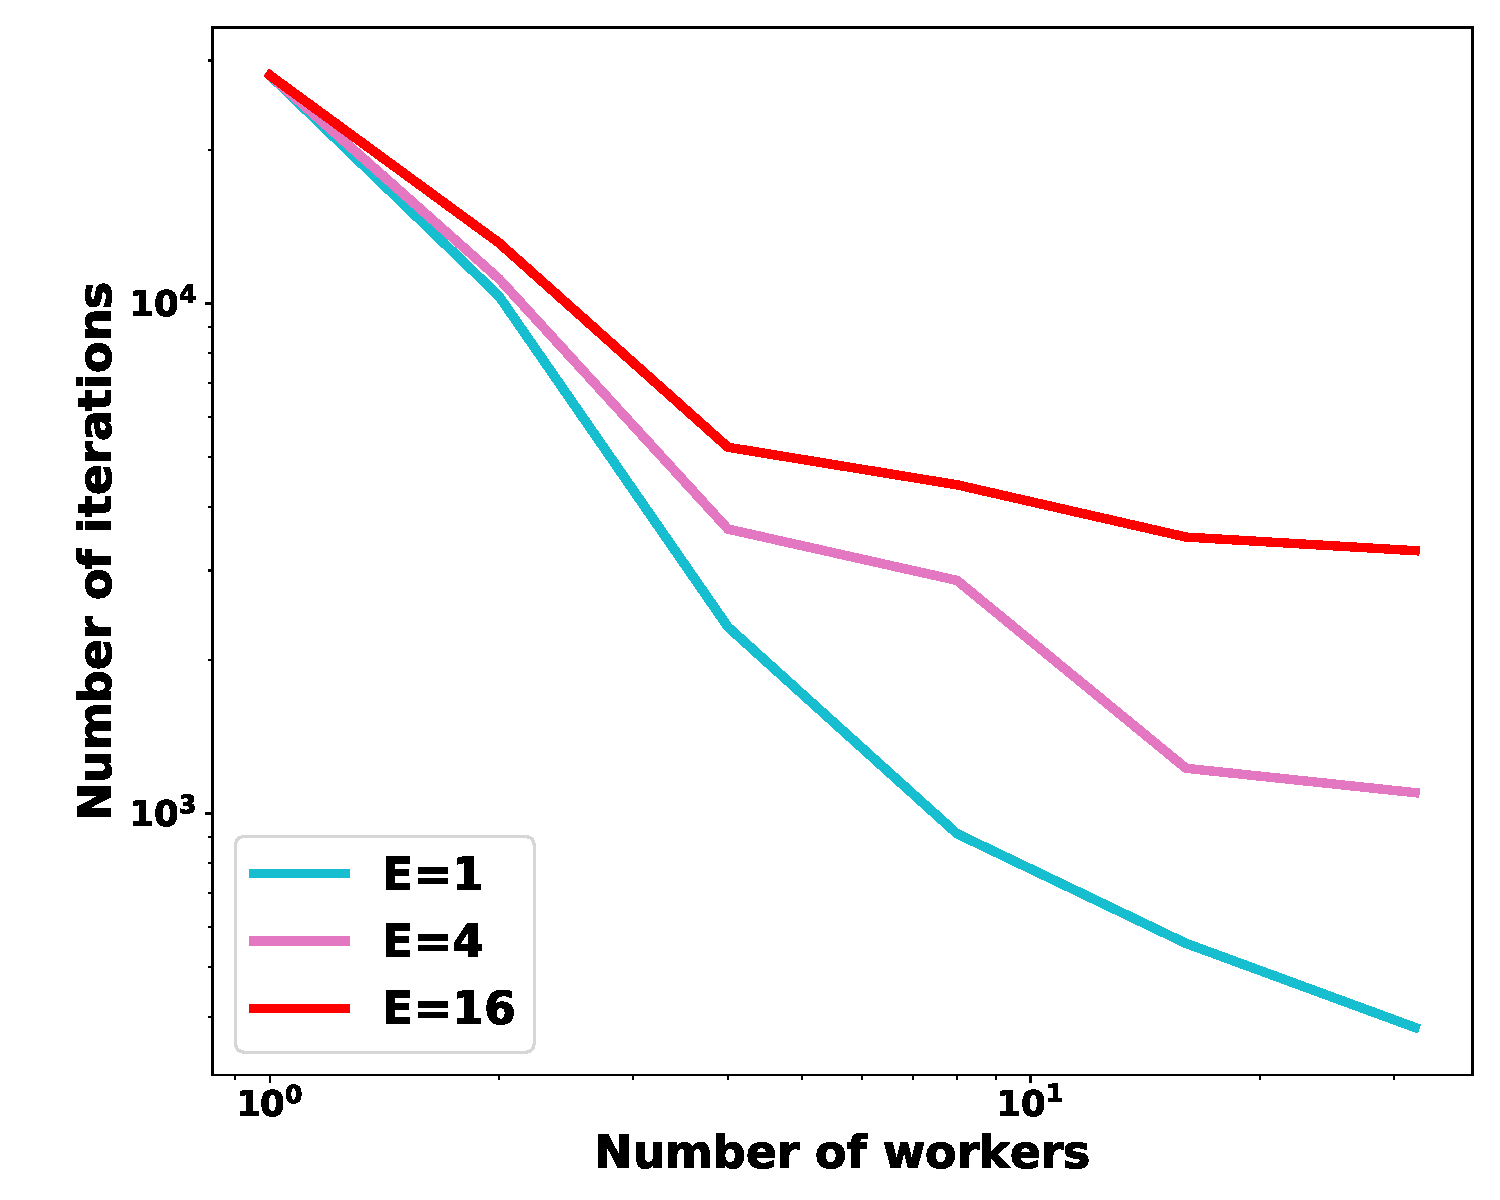
\includegraphics[width=0.33\textwidth]{fig/paper-stronglycvxsmthspeedupNodesT-min-w8a-epsilon0131-reg1e-05.pdf} &
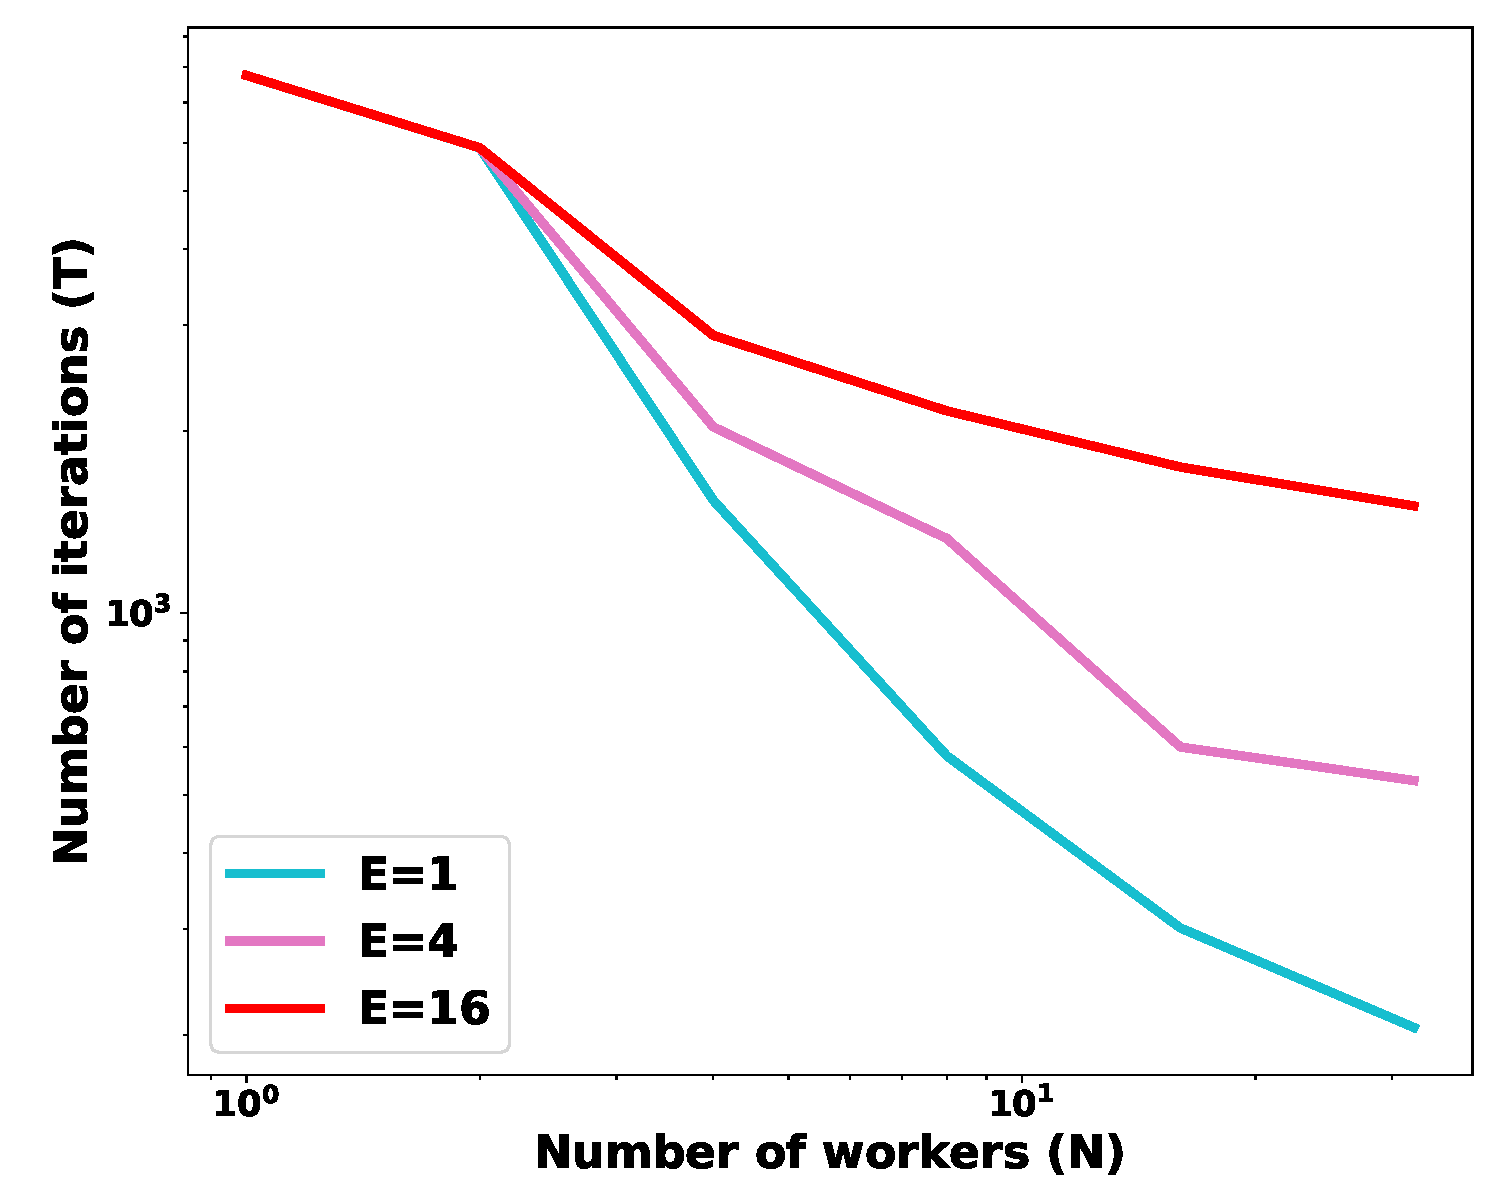
\includegraphics[width=0.33\textwidth]{fig/paper-cvxsmoothspeedupNodesT-min-w8a-epsilon0134-reg0.pdf} &
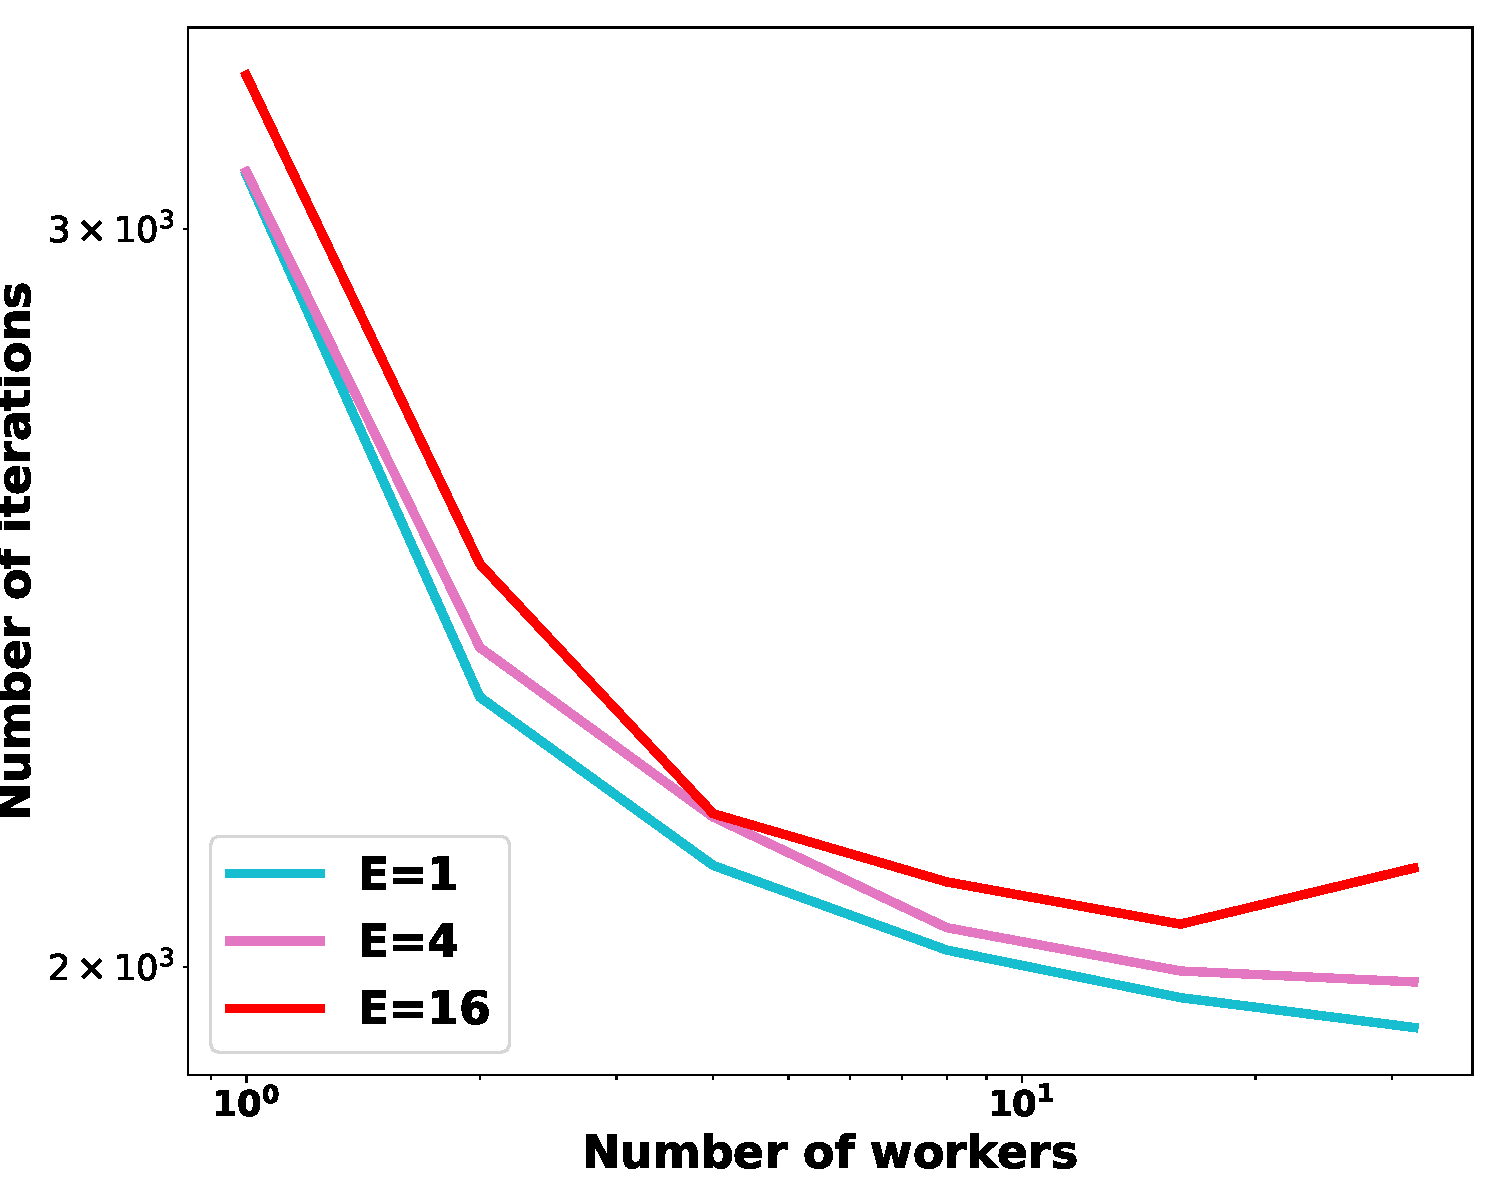
\includegraphics[width=0.33\textwidth]{fig/paper-linregressionspeedupNodesT-min-linearregressionw8a-epsilon002-reg0.pdf}\\
(a) Strongly convex objective & (b) Convex smooth objective & (c) Linear regression
	\end{tabular}
\caption{The linear speedup convergence of FedAvg w.r.t the number of workers. }
\label{fig:speedup}
\end{figure}

\begin{figure}
\centering
	\begin{tabular}{ccc}
	\hspace{-2em} 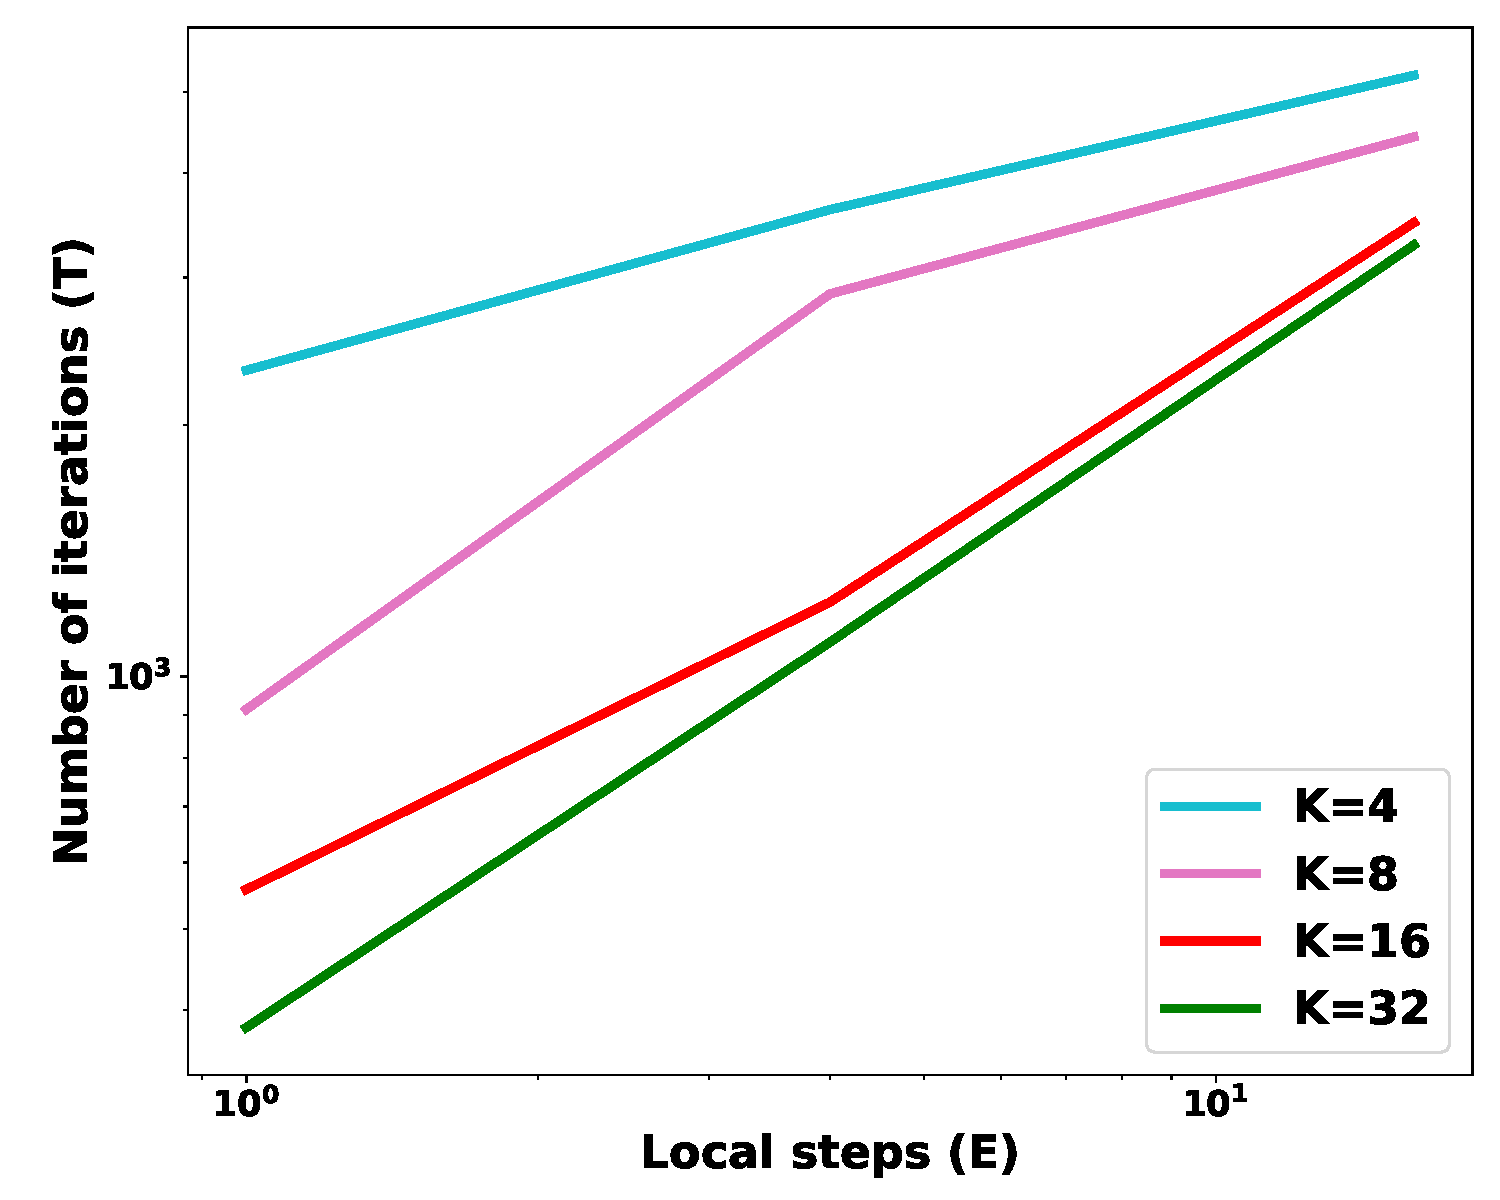
\includegraphics[width=0.33\textwidth]{fig/paper-stronglycvxsmthspeedupEpochsT-min-w8a-epsilon0131-reg1e-05.pdf} &
	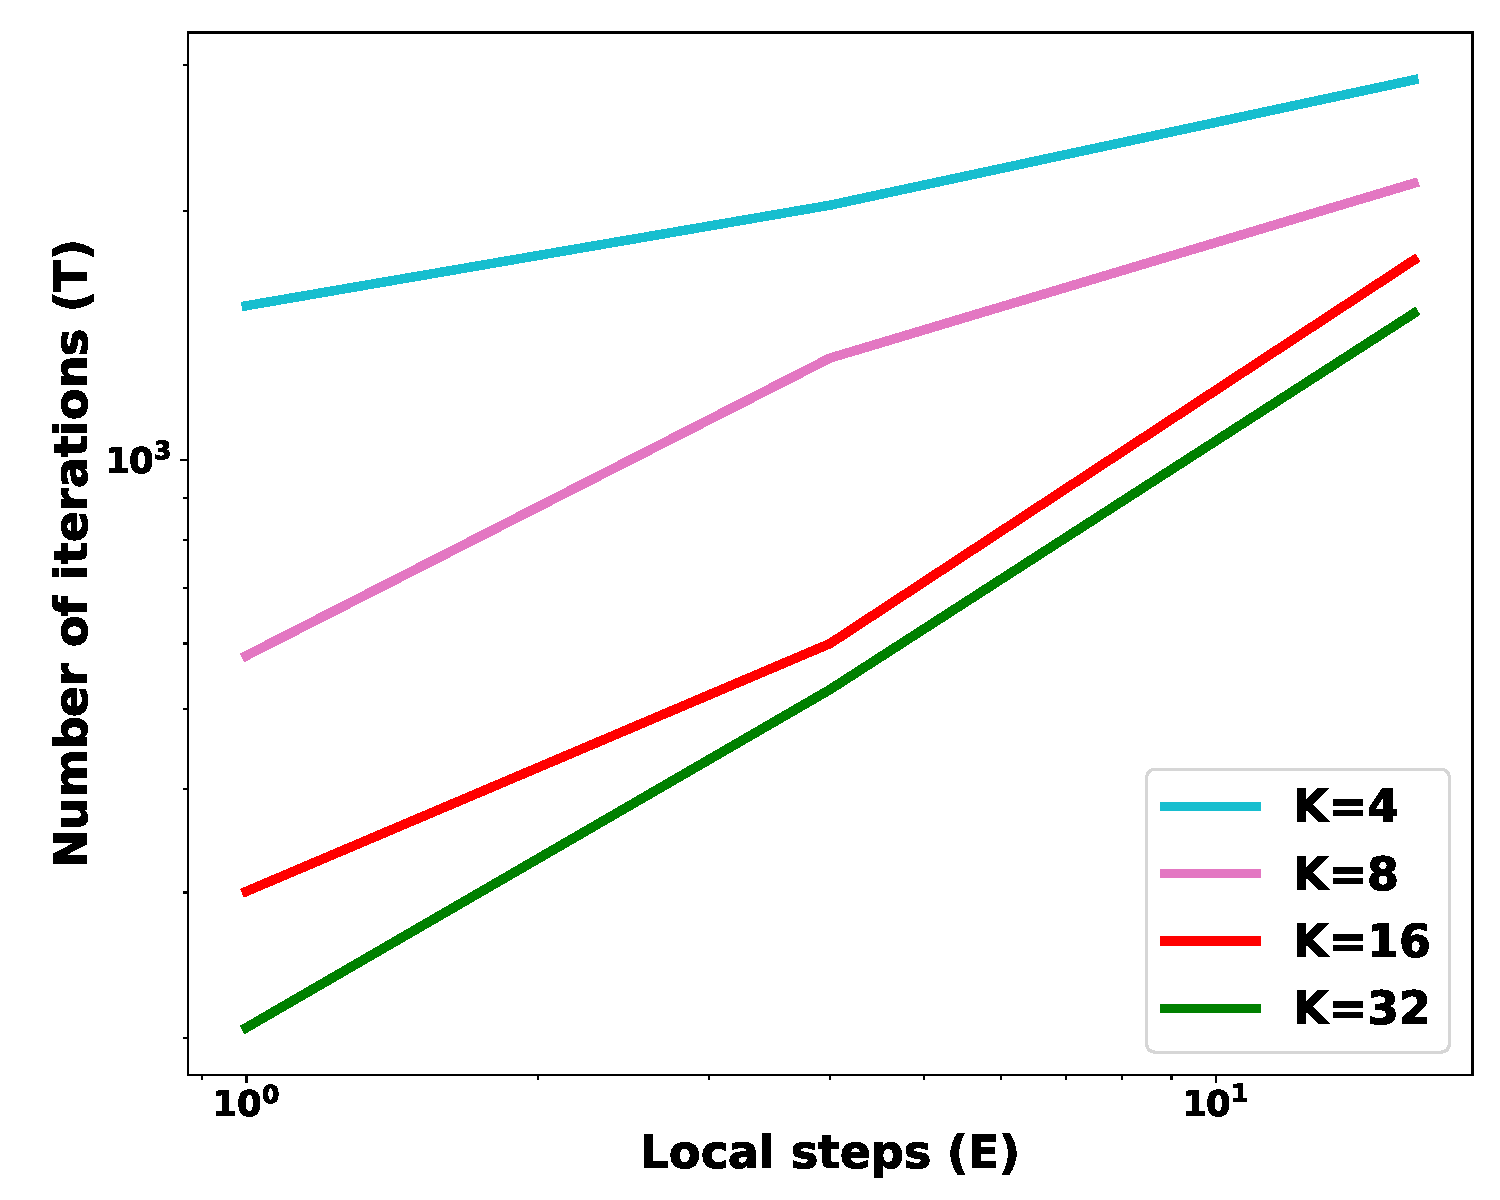
\includegraphics[width=0.33\textwidth]{fig/paper-cvxsmoothspeedupEpochsT-min-w8a-epsilon0134-reg0.pdf} & 
	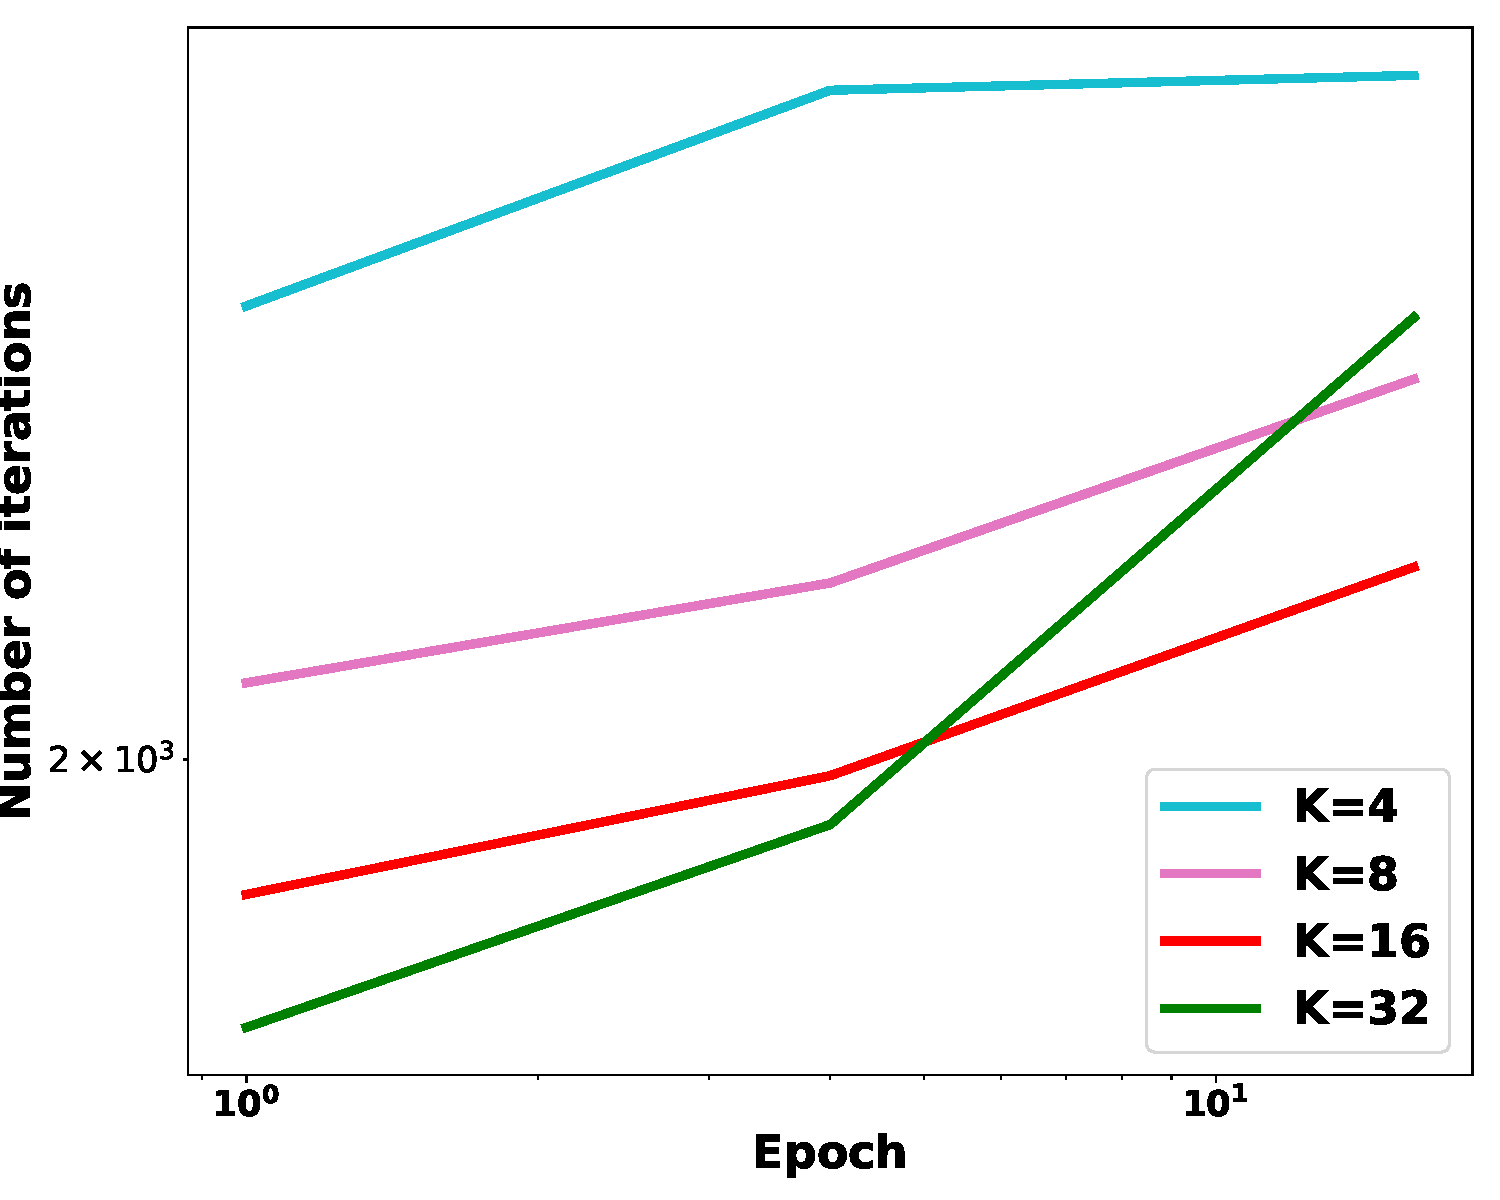
\includegraphics[width=0.33\textwidth]{fig/paper-linregressionspeedupEpochsT-min-linearregressionw8a-epsilon002-reg0.pdf} \\
	\hspace{-2em} 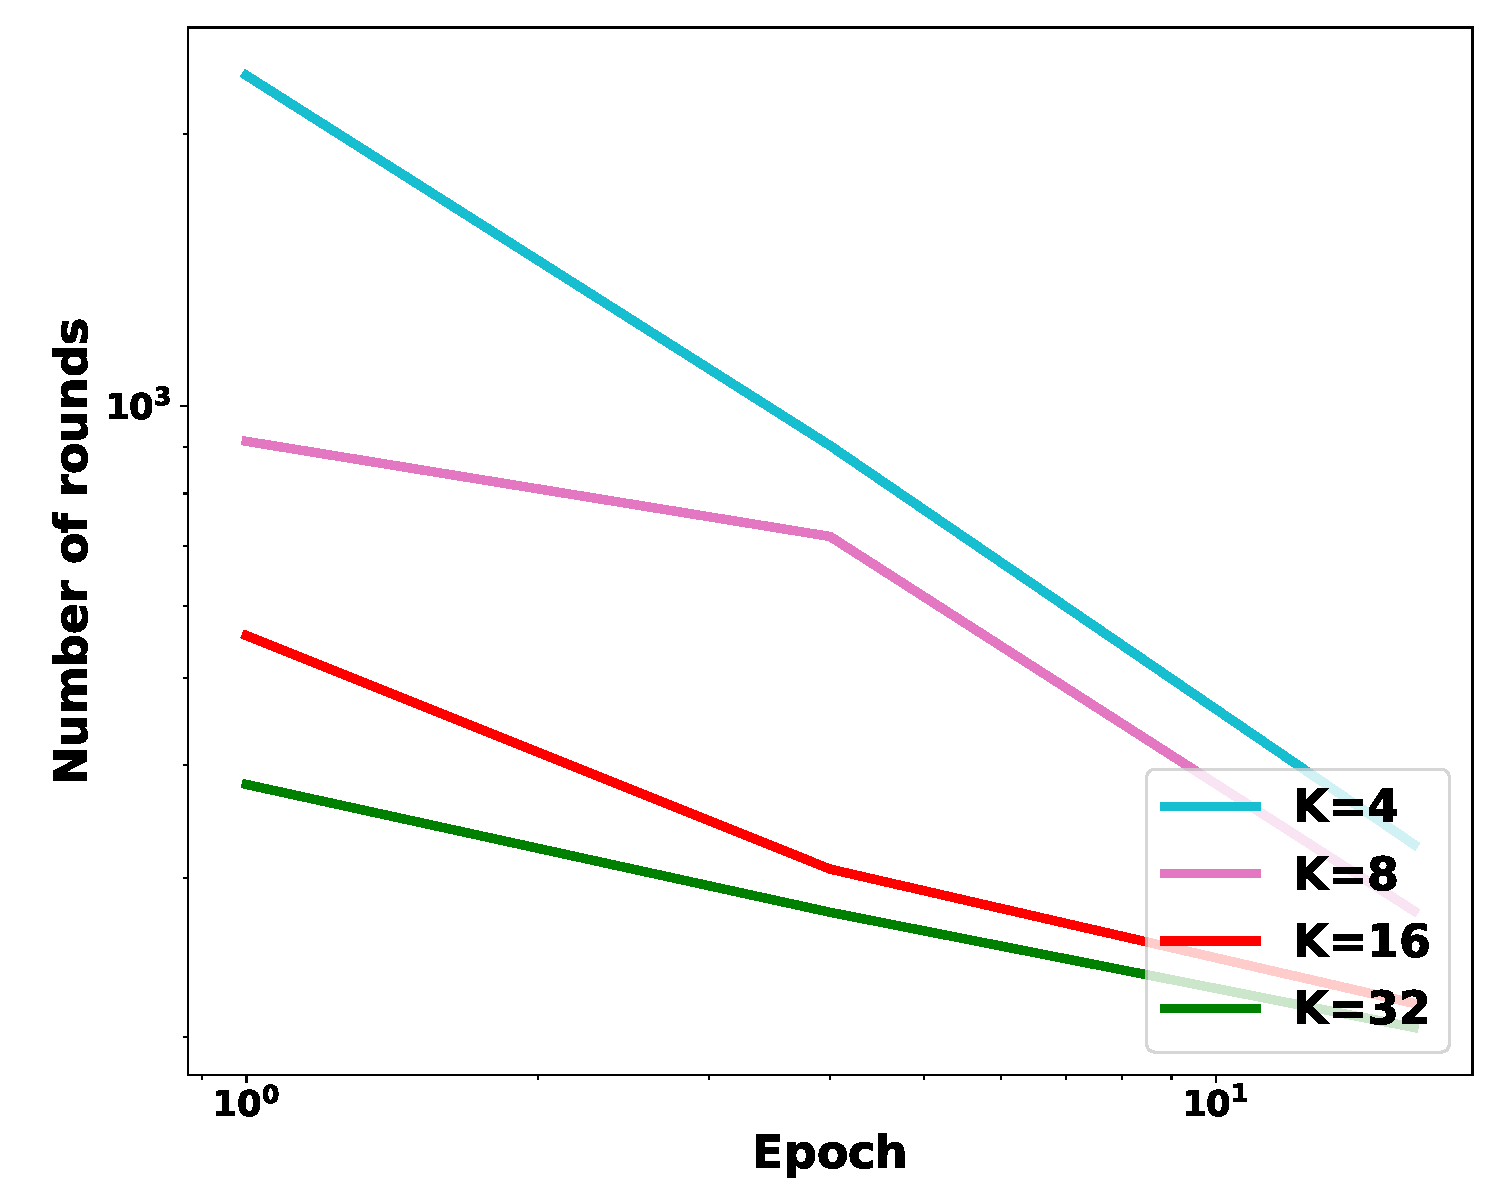
\includegraphics[width=0.33\textwidth]{fig/paper-stronglycvxsmthspeedupEpochsRounds-min-w8a-epsilon0131-reg1e-05.pdf} &
	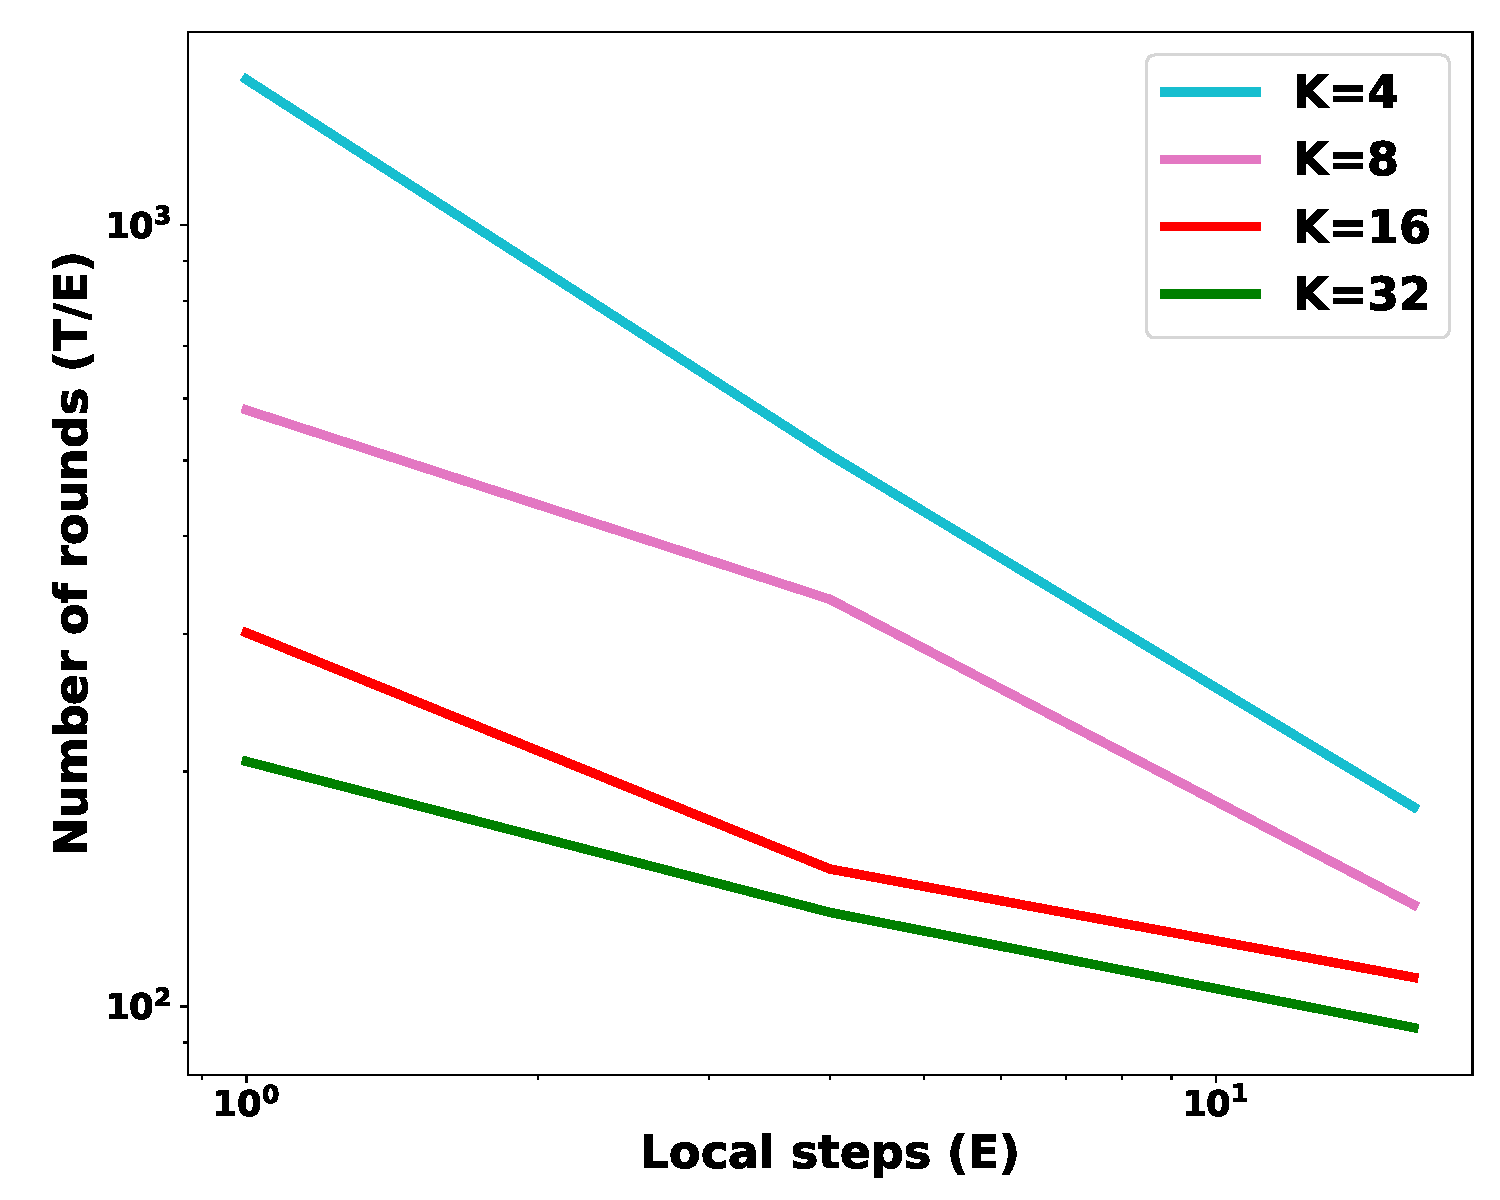
\includegraphics[width=0.33\textwidth]{fig/paper-cvxsmoothspeedupEpochsRounds-min-w8a-epsilon0134-reg0.pdf} & 
	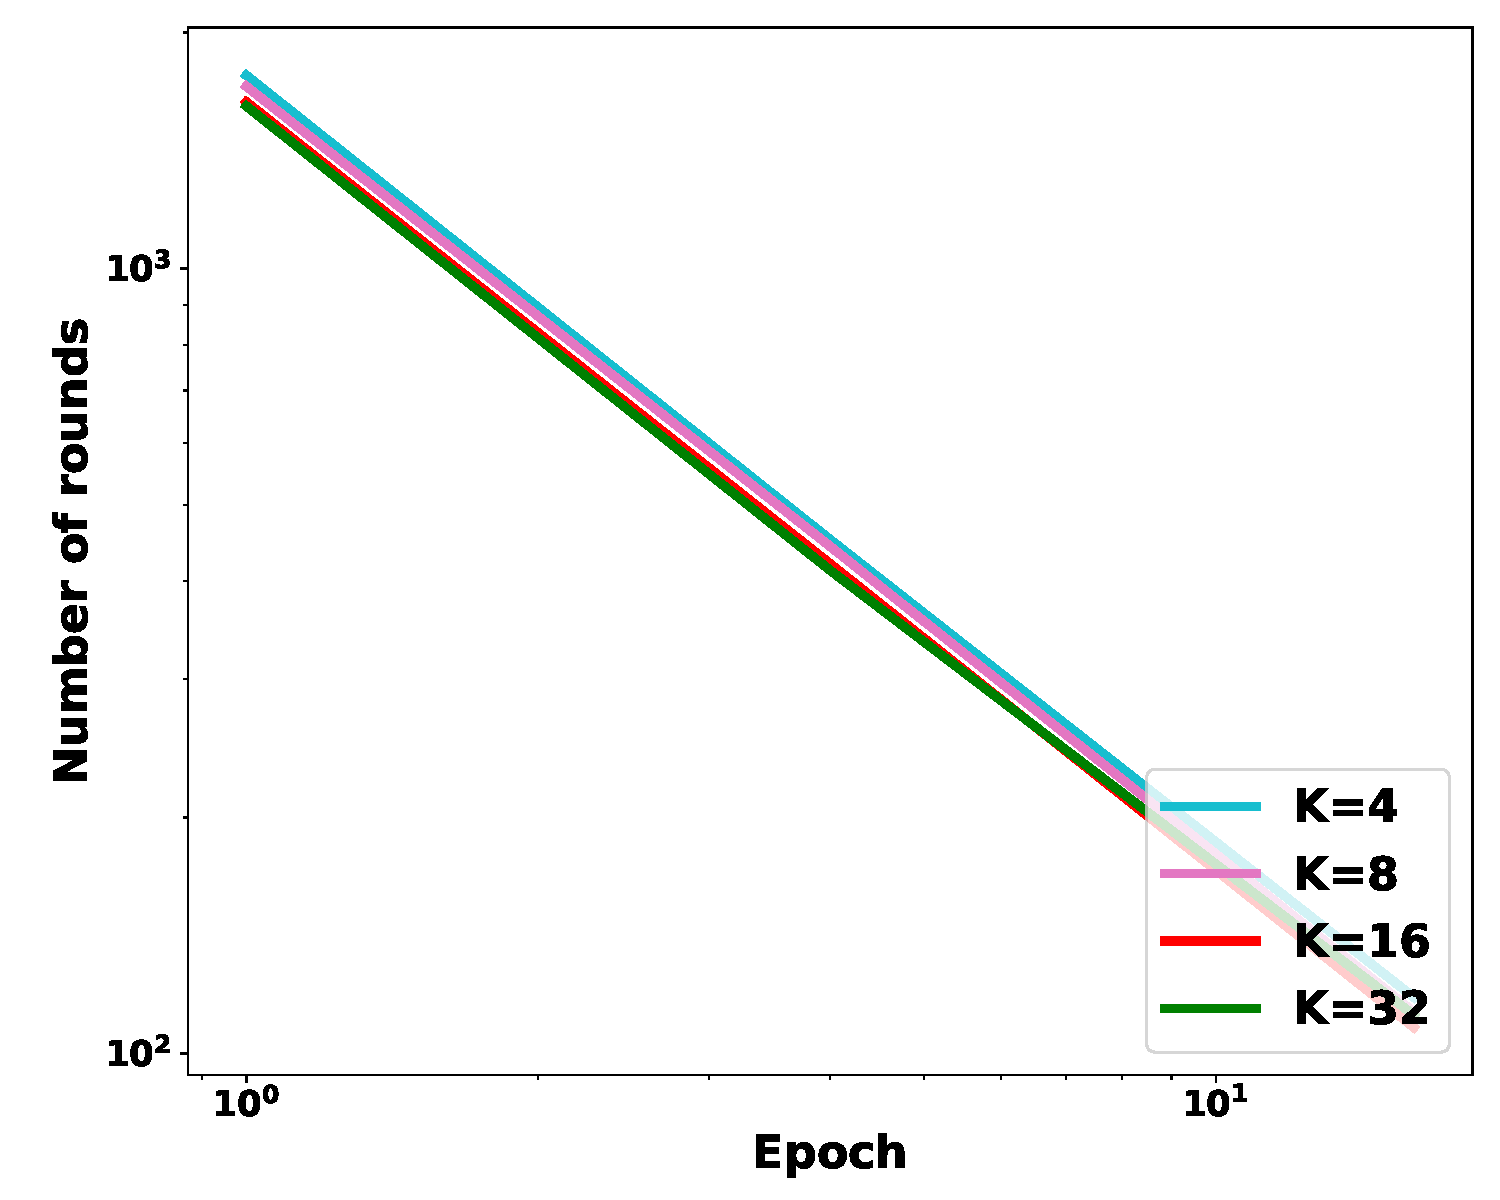
\includegraphics[width=0.33\textwidth]{fig/paper-linregression-newspeedupEpochsRounds-min-linearregressionw8a-epsilon002-reg0.pdf} \\
(a) Strongly convex objective & (b) Convex smooth objective & (c) Linear regression
	\end{tabular}
\caption{The convergence of FedAvg w.r.t the number of epochs. }
\label{fig:e}
\end{figure}

\begin{figure}
\centering
	\begin{tabular}{ccc}
	\hspace{-2em}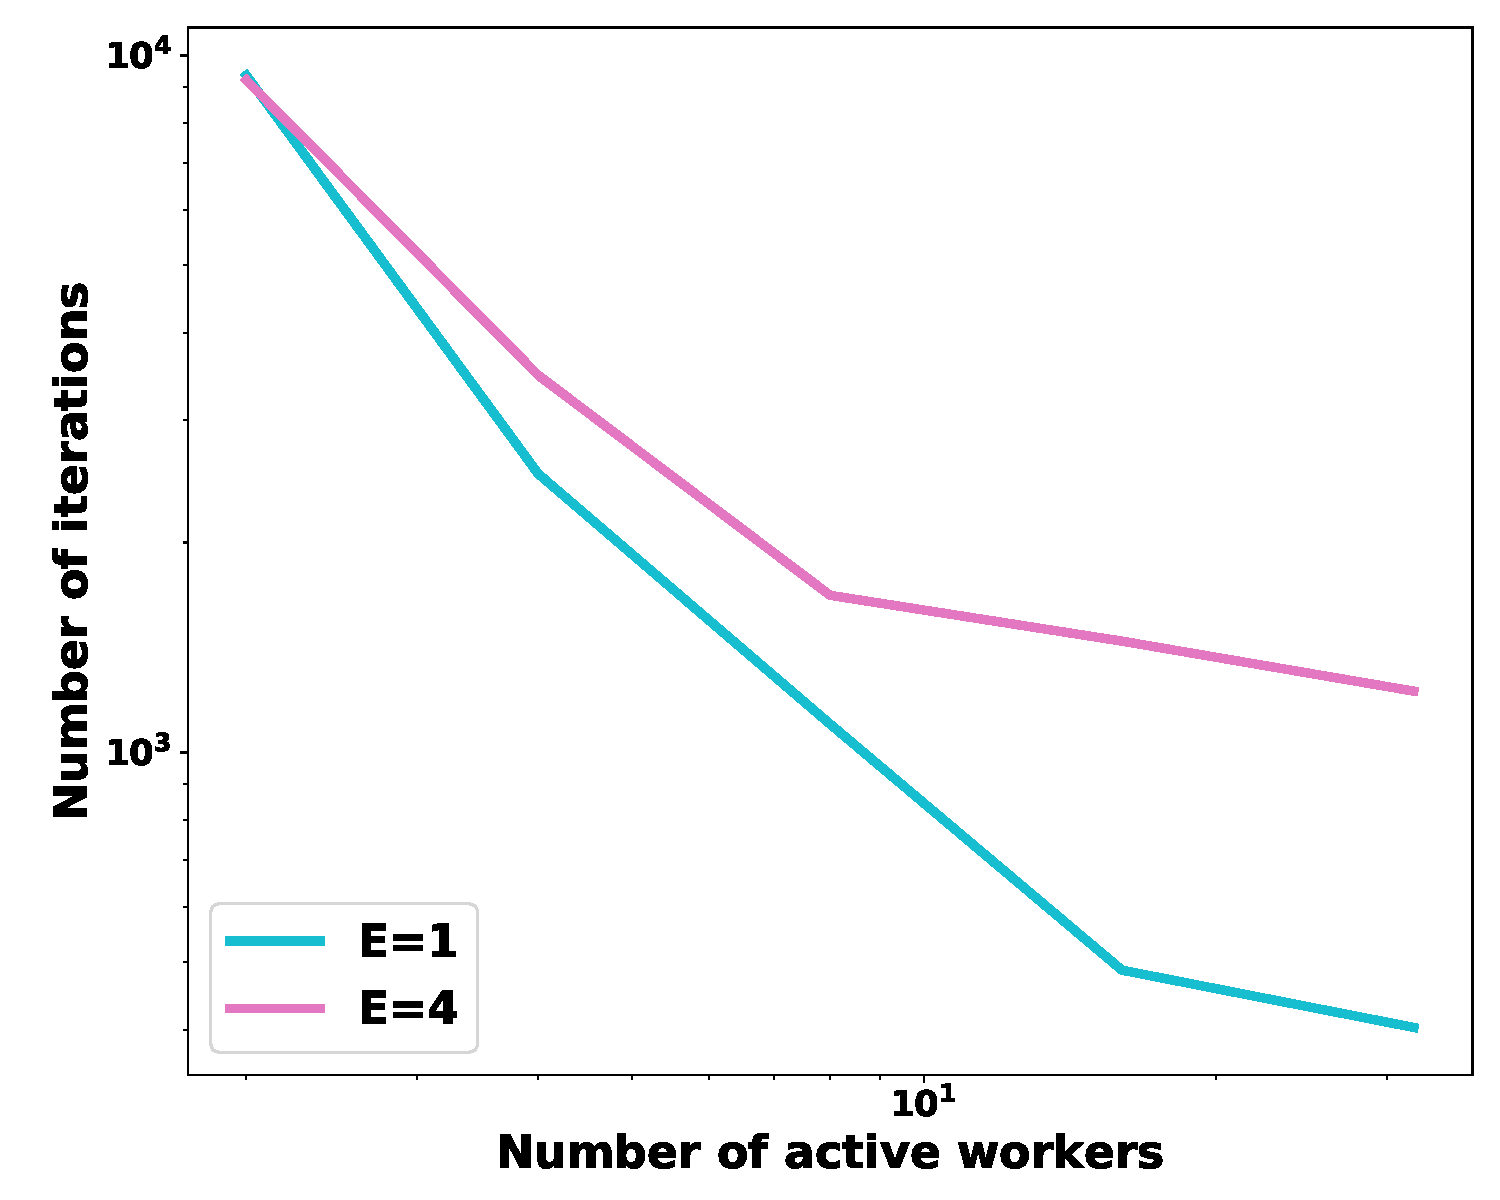
\includegraphics[width=0.33\textwidth]{fig/paper-partialstronglycvxsmthspeedupNodesT-min-w8a-epsilon0131-reg1e-05.pdf} &
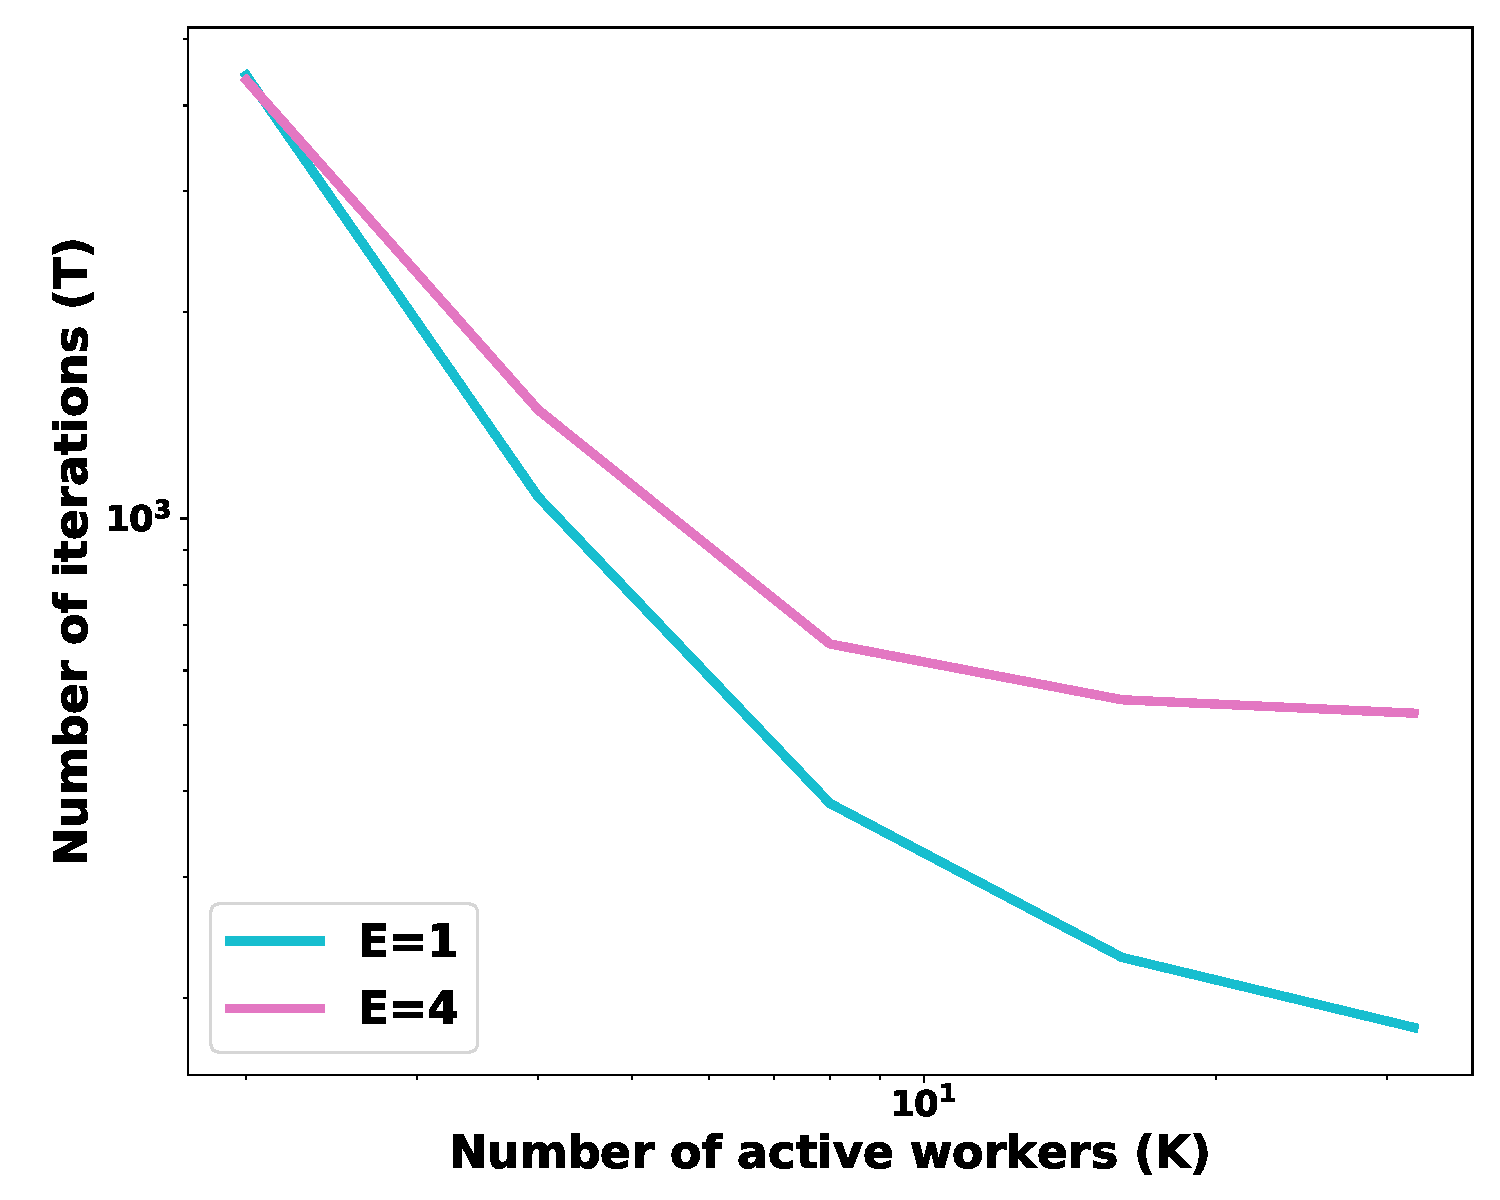
\includegraphics[width=0.33\textwidth]{fig/paper-partialcvxsmoothspeedupNodesT-min-w8a-epsilon0134-reg0.pdf} &
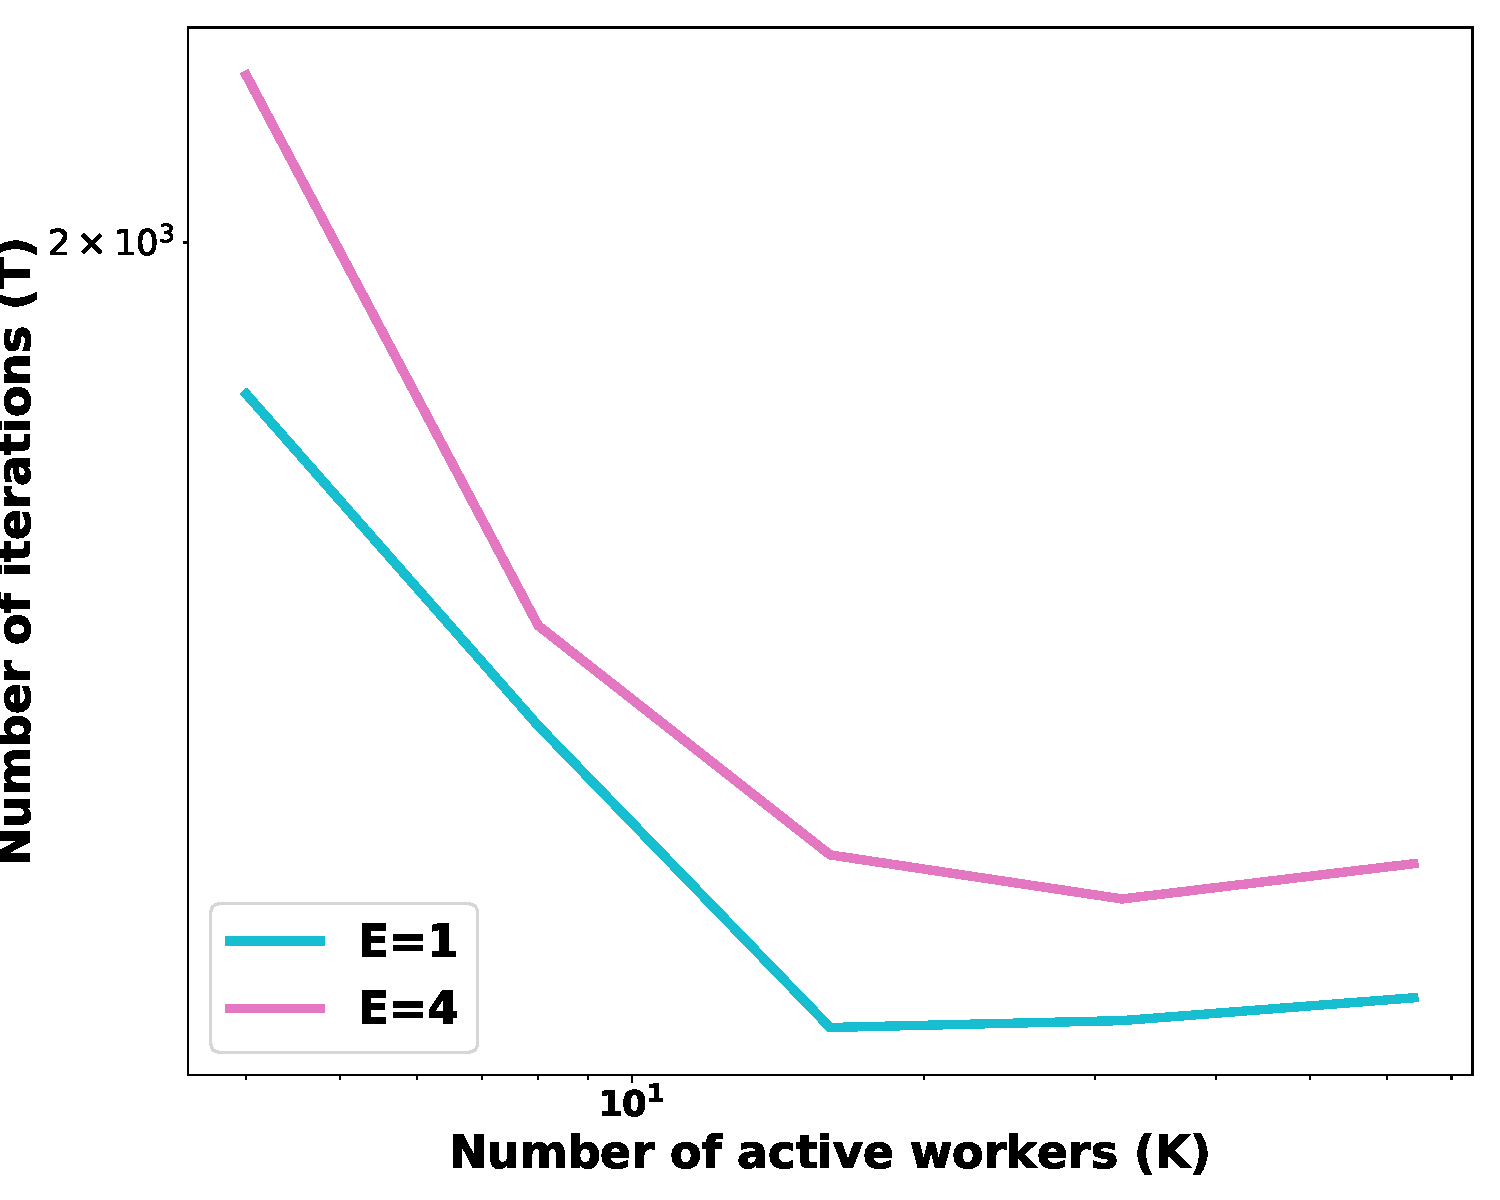
\includegraphics[width=0.33\textwidth]{fig/paper-partiallinregressionspeedupNodesT-min-linearregressionw8a-epsilon002-reg0.pdf}\\
(a) Strongly convex objective & (b) Convex smooth objective & (c) Linear regression
	\end{tabular}
\caption{The linear speedup convergence of FedAvg w.r.t the number of active workers. }
\label{fig:partial}
\end{figure}


\begin{figure}
\centering
\begin{tabular}{ccc}
\hspace{-2em}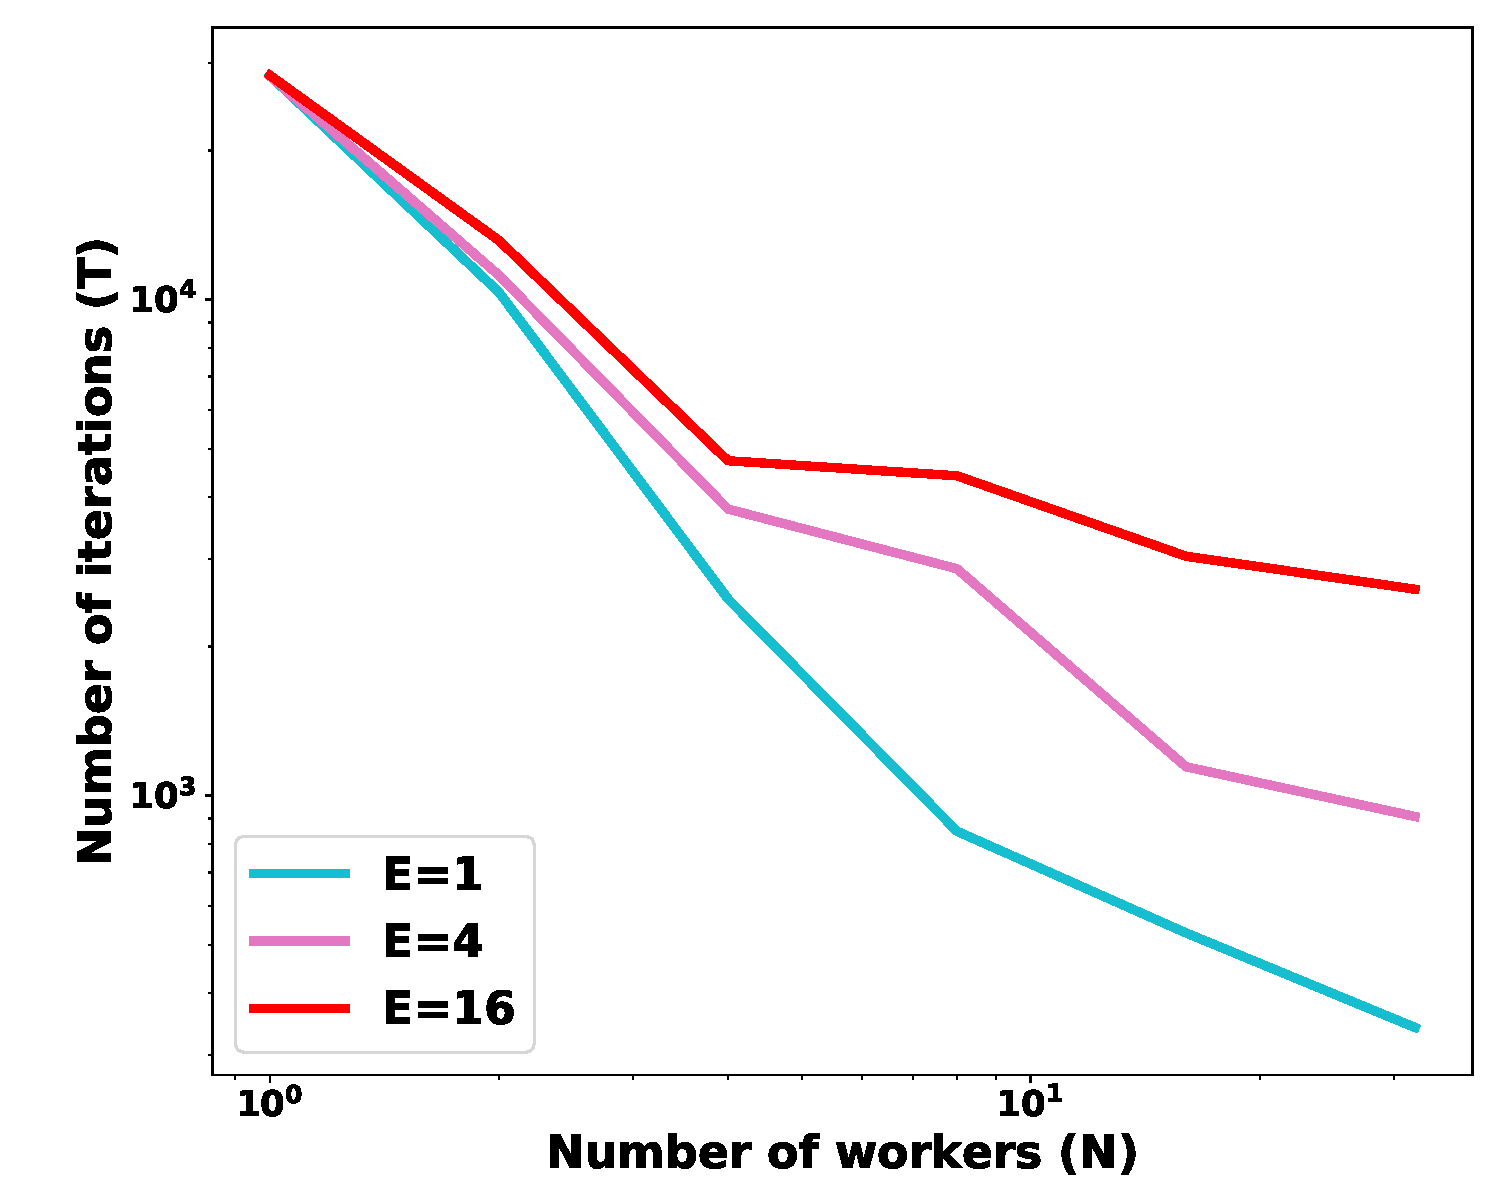
\includegraphics[width=0.33\textwidth]{fig/paper-nesterovspeedupNodesT-min-w8a-epsilon0131-reg1e-05.pdf} & 
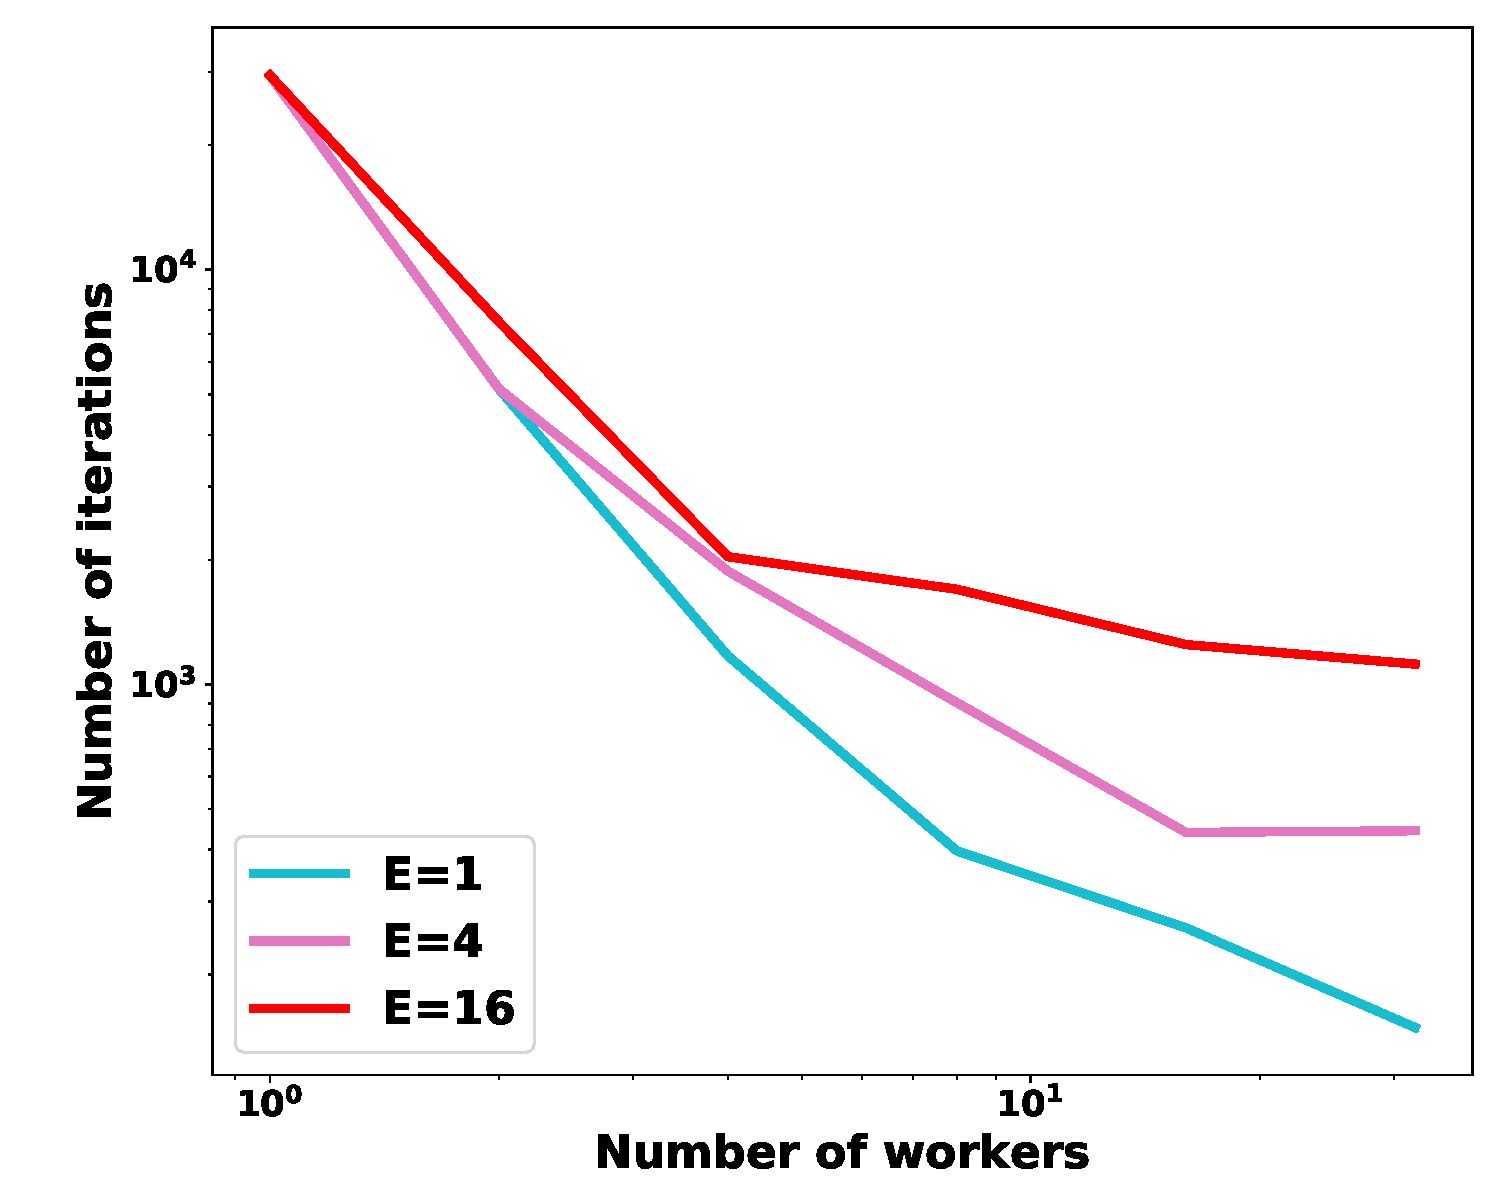
\includegraphics[width=0.33\textwidth]{fig/paper-nesterovspeedupNodesT-min-w8a-epsilon0134-reg0.pdf}
& 
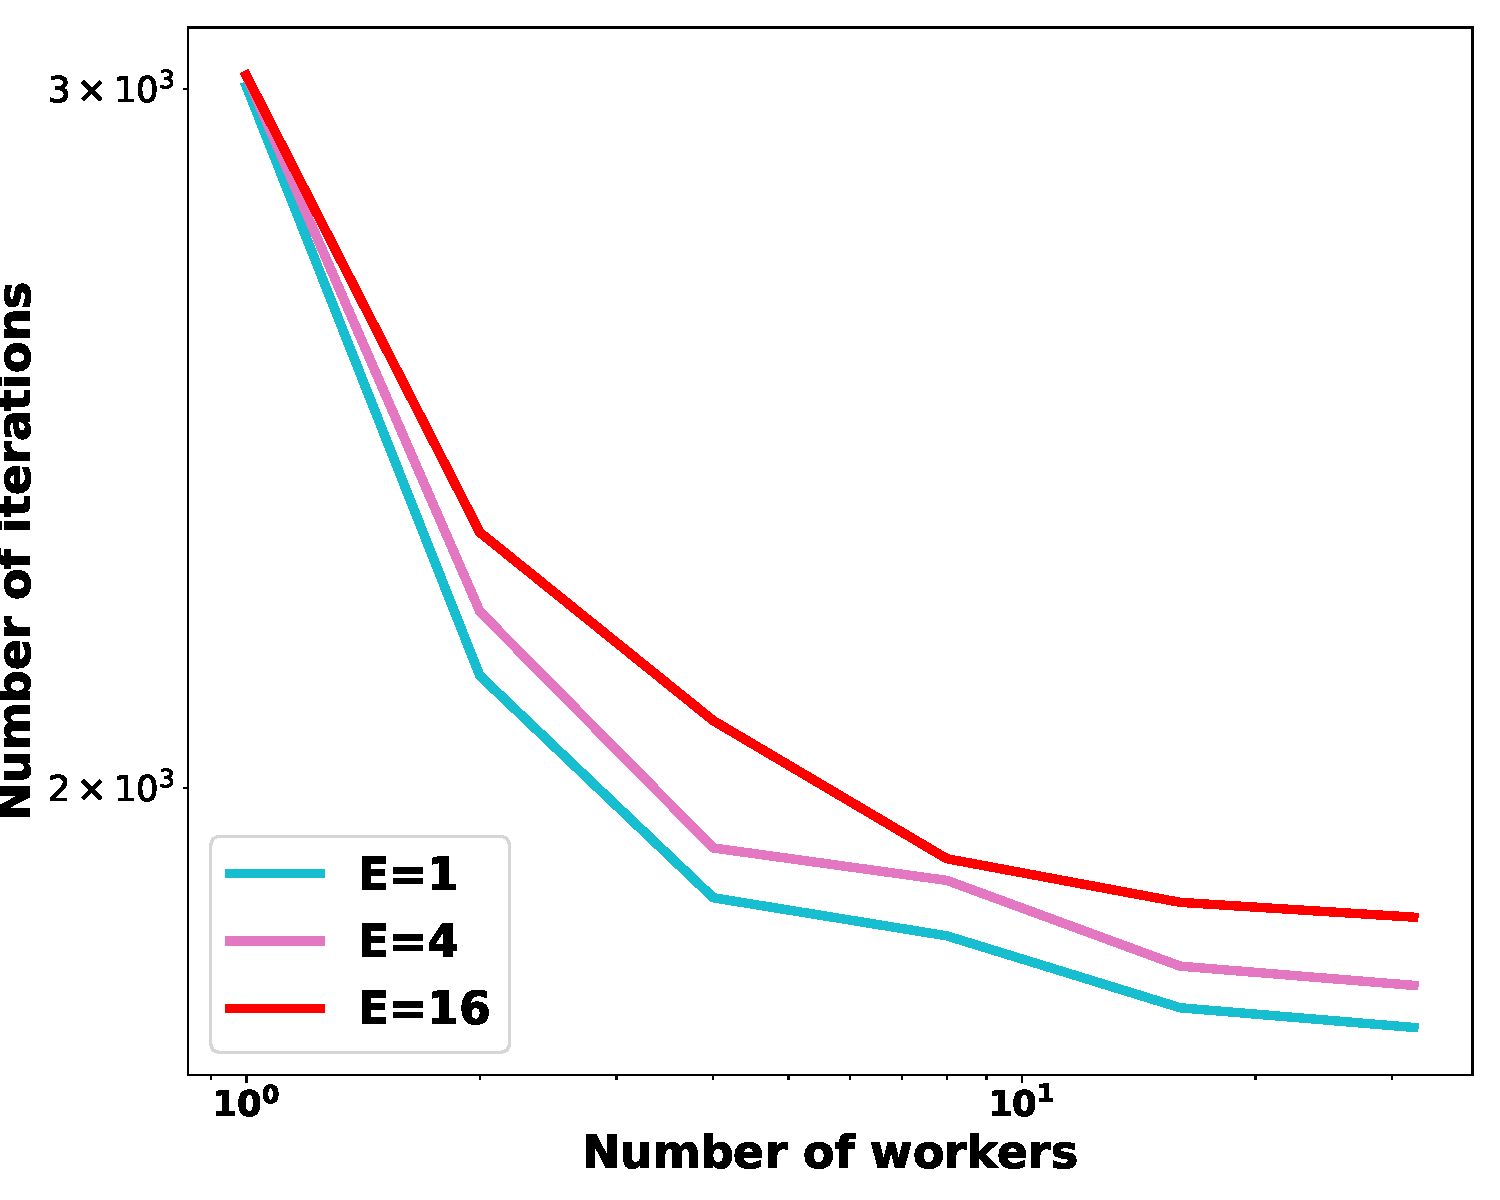
\includegraphics[width=0.33\textwidth]{fig/paper-lrnesterovspeedupNodesT-min-linearregressionw8a-epsilon002-reg0.pdf}\\
(a) Strongly convex objective & (b) Convex smooth objective & (c) Linear regression
	\end{tabular}
\caption{The linear speedup convergence of Nesterov accelerated FedAvg w.r.t the number of workers. }
\label{fig:nesterov}
\end{figure}



% !TEX ROOT=./main.tex

\section{Conclusions}
\begin{comment}
This paper provides a comprehensive and unified analysis of the convergence rate of FedAvg
and its accelerated variants in a general federated learning problem with heterogeneous local data and partial participation. We show that both Nesterov accelerated FedAvg and FedAvg
can achieve {\small{$\cO(\frac{1}{\sqrt{NT}})$}} linear speedup convergence for convex smooth problems and {\small{$\cO(\frac{1}{NT})$}} convergence for strongly 
convex smooth problems. In addition, we show that the local steps for stronlgy convex and convex smooth problems can be as large as {\small{$\cO(\sqrt{\frac{T}{N}})$}}, which can substantially save communication cost comparing to prior results. 
Furthermore, this work also makes algorithmic contributions. We not only prove that FedAvg can achieve exponential convergence for overparameterized strongly convex smooth problems, but also propose the MaSS accelerated Fedavg algorithm, which has provable speedup in convergence rate over FedAvg on quadratic problems. Last but not least, we empirically
verify the linear speedup of FedAvg and Nesterov accelerated FedAvg for strongly convex, convex smooth, and linear regression problems. The empirical results are well-aligned with our theories.		
\end{comment}
\vspace{-1em}
This paper provides a comprehensive and unified analysis of the convergence of FedAvg
and its accelerated variants in a general federated learning problem with heterogeneous local data and partial participation. 
We show that both Nesterov accelerated FedAvg and FedAvg can achieve linear speedup convergence for convex smooth problems and strongly 
convex smooth problems. We further prove that FedAvg can achieve geometric convergence for overparameterized strongly convex smooth problems. Last but not least, extensive empirical 
evaluations demonstrate the linear speedup of FedAvg and accelerated FedAvg under various settings.	



% !TEX ROOT=./main.tex

% Broader impact: Authors are asked to include a section in their submissions discussing the broader impact of their work, including possible societal consequences — -both positive and negative.
\section{Broader impact}
With the widespread use of mobile devices, the powerful sensors
collected enormous amount of data empowered with machine learning
solutions can transform people's life in many aspects. The proper
data integration can produce positive social
impact in terms of better personalization~\cite{fallah2020personalized}, more efficient information solicitation~\cite{chen2018federated}, and enhanced service~\cite{47586}.

In the meantime, the increasing concerns of security and
privacy leaking from both large companies and the entire society
present significant challenges of proper utilization of local
data. This trade-off between efficiency and privacy/security
lies in the center of many industrial applications, including 
but not limited to recommendation systems~\cite{chen2018federated}, virtual assistants~\cite{lamautonomy}, and mobile keyboard prediction~\cite{47586}.

In this work, we establish solid theoretical foundations for federated
learning that achieves efficiency and privacy at the same time. 
On one hand, the data is isolated in each local devices, thus prevent
the potential leakage of private information. On the other hand, the
convergence rates can be improved substantially if the number of
active local devices increases. In conclusion, our work 
shows a faithful pathway to simultaneously secure people's privacy and improve
users' experience.




\newpage
\bibliographystyle{plain}
\bibliography{ref.bib}

\appendix
% !TEX ROOT=./main.tex
% !TEX ROOT=./main.tex

\section{Additional Notations}
\label{sec:app:notations}
In this section, we introduce additional notations that are used throughout
the proof. Following common practice~\cite{stich2018local,li2019convergence}, we define two virtual sequences $\overline{\mathbf{v}}_{t}$ and $\overline{\mathbf{w}}_{t}$. For full device participation and $t \notin \cI_E$,
$\ov{v}_t = \ov{w}_t =\sum_{k=1}^{N} p_{k} \mathbf{v}_{t}^{k}$. For partial participation, $t \in \cI_E$, $\ov{w}_t \neq \ov{v}_t$ since $\ov{v}_t=\sum_{k=1}^{N} p_{k} \mathbf{v}_{t}^{k}$ while $\ov{w}_t=\sum_{k\in \cS_t}\mathbf{w}_{t}^{k}$. However, we can
set unbiased sampling strategy such that $ \EE_{\cS_t} \ov{w}_t = \ov{v}_t$.
$\overline{\mathbf{v}}_{t+1}$ is one-step SGD from $\overline{\mathbf{w}}_{t}$. 
\begin{align}
\overline{\mathbf{v}}_{t+1}=\overline{\mathbf{w}}_{t}-\eta_{t} \mathbf{g}_{t}	\label{eq:vbar}
\end{align}
% $t+1 \in \cI_E$, we can fetch $\overline{\vw}_{t+1}$, we can communicate $\overline{\vw}_{t+1}$ to all devices.
where $\vg_{t} = \sum_{k=1}^{N} p_{k} \vg_{t,k} $ is one-step stochastic gradient, averaged over all devices. 
\begin{align}
\vg_{t,k} \left\{\begin{array}{ll} 
 = \nabla F_{k}\left(\mathbf{w}_{t}^{k},\xi_{t}^{k} \right)  &  \text{smooth}\\
 \in \partial F_{k}\left(w_{t}^{k}, \xi_{t}^{k}\right)  & \text{non-smooth}
 \end{array}\right.
\end{align}
Similarly, we denote the expected one-step gradient $\ov{g}_{t}= \EE_{\xi_t}[\vg_t] = \sum_{k=1}^{N} p_{k} \EE_{\xi_{t}^{k}} \vg_{t,k}$, where
\begin{align}
\EE_{\xi_{t}^{k}} \vg_{t,k}  \left\{\begin{array}{ll} 
 = \nabla F_{k}\left(\mathbf{w}_{t}^{k}\right)  &  \text{smooth}\\
 \in \partial F_{k}\left(w_{t}^{k}\right)  & \text{non-smooth}
 \end{array}\right.
\end{align}
and $\xi_t = \{\xi_t^k\}_{k=1}^N$ denotes random samples at all devices at time step $t$. 
Since in this work, we also consider the case of partial participation. The sampling
strategy to approximate the system heterogeneity can also affect the convergence. Here we
follow the prior arts~\cite{haddadpour2019convergence} considering two types of sampling
schemes. 
The sampling scheme I establishes $\cS_{t+1}$ by i.i.d. sampling the devices with replacement,
in this case the upper bound of expected square norm of $\ov{w}_{t+1} - \ov{v}_{t+1}$ is given by:
\begin{align}
\EE_{\cS_{t+1}}\left\|\ov{w}_{t+1} - \ov{v}_{t+1}\right\|^2	\leq \frac{4}{K} \eta_t^2 E^2G^2
\end{align}
The sampling scheme II establishes $\cS_{t+1}$ by uniformly sampling all devices without
replacement, in which we have the 
\begin{align}
\EE_{\cS_{t+1}}\left\|\ov{w}_{t+1} - \ov{v}_{t+1}\right\|^2	\leq \frac{4(N - K)}{K(N-1)} \eta_t^2 E^2G^2
\end{align}
We denote this upper bound as follows for concise presentation. 
\begin{align}
	\EE_{\cS_{t+1}}\left\|\ov{w}_{t+1} - \ov{v}_{t+1}\right\|^2 \leq  \eta_t^2 C
	\label{eq:partialsample}
\end{align}
% !TEX ROOT=./main.tex


\section{Comparison of convergence rates}

\begin{table}
\centering
\begin{tabular}{|c|c|c|}\hline 
	Algorithm \textbackslash Setting            & Strongly Convex        & Convex \\ \hline \hline
	FedAvg                         & $\cO(\frac{1}{NT}+\frac{E^{2}}{T^{2}})$    &  $\mathcal{O}\left(\frac{1}{\sqrt{NT}}+\frac{NE^{2}}{T}\right)$       \\ \hline
	Nesterov accelerated FedAvg    & $\cO(\frac{1}{NT}+\frac{E^{2}}{T^{2}})$    & $\mathcal{O}\left(\frac{1}{\sqrt{NT}}+\frac{NE^{2}}{T}\right)$       \\ \hline
\end{tabular}
\caption{The summary of the convergence results in this work.}
\end{table}

\begin{table}
\centering
{\small
\begin{tabular}{|c|c|c|c|c|c|c|}
\hline Reference                 & Convergence rate    & E                           & Non-IID & Participation & Extra Assumptions  		  & Setting  \\ \hline\hline 
\cite{li2019convergence}         & $\cO(\frac{E^2}{T})$& $\cO(1)$                    & \cmark  & Partial       & Bounded gradient   		  & Strongly convex  \\ \hline
\cite{haddadpour2019convergence} & $\cO(\frac{1}{KT})$ & $\cO(K^{1/3}T^{2/3})^*$     & \cmark  & Partial       & Bounded gradient diversity   & Strongly convex  \\ \hline
This work                        & $\cO(\frac{1}{KT})$ & $\cO(N^{-1/2}T^{1/2})^{**}$ & \cmark  & Partial       & Bounded gradient             & Strongly convex  \\\hline\hline
\cite{zanette2019tighter}        &                     &                             & \cmark  & Partial       & Bounded gradient             & Convex  \\\hline\hline

% Khaled et al. (2020) & & & \\
% Li et al. (2019) & & & \\
% this work & $\mathcal{O}\left(\frac{\kappa\nu_{\max}^{2}\sigma^{2}}{NT\mu}+\frac{\kappa E^{2}G^{2}}{KT\mu}+\frac{\kappa^{2}E^{2}G^{2}}{T^{2}\mu}\right)$ &  &  \\
\end{tabular}
}
\caption{$^*$ This $E$ is obtained under i.i.d. setting. 
         $^{**}$: This $E$ is obtained under full participation setting.}
\end{table}







\section{A unified framework for FedAvg analysis}

In this section, we provide a unified proof framework for FedAvg and its accelerated variants. 



\section{Technical lemmas}


To facilitate reading, we first summarize some basic properties of $L$-smooth and $\mu$-strongly
convex functions, found in e.g.~\cite{rockafellar1970convex}, which are used in various steps of proofs in the appendix. 
\begin{lemma}
	Let $F$ be a convex $L$-smooth function. Then we have the following
	inequalities:
	
	1. Quadratic upper bound: $0\leq F(\vw)-F(\vw')-\langle\nabla F(\vw'),\vw-\vw'\rangle\leq\frac{L}{2}\|\vw-\vw'\|^{2}$. 
	
	2. Coercivity: $\frac{1}{L}\|\nabla F(\vw)-\nabla F(\vw')\|^{2}\leq\langle\nabla F(\vw)-\nabla F(\vw'),\vw-\vw'\rangle$.
	
	3. Lower bound: $F(\vw)\geq F(\vw')+\langle\nabla F(\vw'),\vw-\vw'\rangle+\frac{1}{2L}\|\nabla F(\vw)-\nabla F(\vw')\|^{2}$.
	In particular, $\|\nabla F(\vw)\|^{2}\leq2L(F(\vw)-F(\vw^{\ast}))$.
	
	4. Optimality gap: $F(\vw)-F(\vw^{\ast})\leq$$\langle\nabla F(\vw),\vw-\vw^{\ast}\rangle$.
\label{lem:lsmooth}
\end{lemma}
%
\begin{lemma}
	Let $F$ be a $\mu$-strongly convex function. Then 
	\begin{align*}
	& F(\vw)  \leq F(\vw')+\langle\nabla F(\vw'),\vw-\vw'\rangle+\frac{1}{2\mu}\|\nabla F(\vw)-\nabla F(\vw')\|^{2}\\
	& F(\vw)-F(\vw^{\ast})  \leq\frac{1}{2\mu}\|\nabla F(\vw)\|^{2}
	\end{align*}
\end{lemma}

% older proofs are in files titled sec_
% newer proofs are in files titled app_


\section{Proof of Convergence Results for FedAvg}
\label{sec:app:fedavg}}

\subsection{Strongly Convex Smooth Objectives}
% !TEX ROOT=./supp-main.tex

To convey our proof clearly and highlight the significance of our results comparing to prior work, 
we first state the follow lemmas and defer the proofs of these lemmas latter. 
\begin{lemma}[\textbf{One round progress}] Let $\overline{\mathbf{w}}_{T}=\sum_{k=1}^{N}p_{k}\mathbf{w}_{T}^{k}$,
suppose our functions satisfies Assumptions~\ref{ass:lsmooth},\ref{ass:stroncvx},\ref{ass:boundedvariance},\ref{ass:subgrad2}, and set step size $\alpha_{t}=\frac{1}{4\mu(\gamma+t)}$
	with $\gamma=\max\{32\kappa,E\}$ and $\kappa=\frac{L}{\mu}$, the updates of FedAvg satisfy
	\begin{align*}
	\mathbb{E}\|\ov{w}_{t+1}-\vw^{\ast}\|^{2} & \leq(1-\mu\alpha_{t})\mathbb{E}\|\ov{w}_{t}-\vw^{\ast}\|^{2}+\alpha_{t}^{2}\frac{1}{N}\nu_{max}^{2}\sigma^{2}+5E^{2}L\alpha_{t}^{3}G^{2}.
	\end{align*}
\label{lem:scvxoner}
\end{lemma}

\begin{lemma}[\textbf{Bounding gradient variance (Lemma 2 \cite{li2019convergence})} ]
Given Assumption~\ref{ass:boundedvariance}, the upper bound of gradient variance is given as follows,
\begin{align*}
	\mathbb{E}\|\vg_{t}-\ov{g}_{t}\|^{2} \leq \sum_{k=1}^{N}p_{k}^{2}\sigma_{k}^{2}.
	\end{align*}
\label{lem:bgv}
\end{lemma}

\begin{lemma}[\textbf{Bounding the divergence of $\vw_t^k$ (Lemma 3 \cite{li2019convergence})} ]
Given Assumption~\ref{ass:subgrad2}, $\alpha_t$ is non-increasing and $\alpha_t \leq 2\alpha_{t+E}$ for all $t\geq 0$, we have
	\begin{align*}
	\mathbb{E}\left[\sum_{k=1}^{N}p_{k}\|\ov{w}_{t}-\vw_{t}^{k}\|^{2} \right]\leq 4E^{2}\alpha_{t}^{2}G^{2}.
	\end{align*}
\label{lem:bdw}
\end{lemma}


We first restate Theorem~\ref{th:scvx_sgd} to facilitate reading and then see its proof based on previous lemmas.
\begin{thm}
	Let $\overline{\mathbf{w}}_{T}=\sum_{k=1}^{N}p_{k}\mathbf{w}_{T}^{k}$,
	$\nu_{\max}=\max_{k}Np_{k}$, and set decaying learning rates $\alpha_{t}=\frac{1}{4\mu(\gamma+t)}$
	with $\gamma=\max\{32\kappa,E\}$ and $\kappa=\frac{L}{\mu}$. Then
	under Assumptions~\ref{ass:lsmooth},\ref{ass:stroncvx},\ref{ass:boundedvariance},\ref{ass:subgrad2} with full device participation, 
	\begin{align*}
	\mathbb{E}F(\overline{\mathbf{w}}_{T})-F^{\ast}=\mathcal{O}\left(\frac{\kappa\nu_{\max}^{2}\sigma^{2}/\mu}{NT}+\frac{\kappa^{2}E^{2}G^{2}/\mu}{T^{2}}\right)
	\end{align*}
	and with partial device participation with at most $K$ sampled devices
	at each communication round, 
	\begin{align*}
	\mathbb{E}F(\overline{\mathbf{w}}_{T})-F^{\ast}=\mathcal{O}\left(\frac{\kappa E^{2}G^{2}/\mu}{KT}+\frac{\kappa\nu_{\max}^{2}\sigma^{2}/\mu}{NT}+\frac{\kappa^{2}E^{2}G^{2}/\mu}{T^{2}}\right)
	\end{align*}
\end{thm}

\begin{proof}
	The proof builds on ideas from~\cite{li2019convergence}. The first step is to observe that the $L$-smoothness of $F$ provides
	the upper bound
	\begin{align*}
	\mathbb{E}(F(\ov{w}_{t}))-F^{\ast} & \leq\frac{L}{2}\mathbb{E}\|\ov{w}_{t}-\vw^{\ast}\|^{2}
	\end{align*}
	and bound $\mathbb{E}\|\ov{w}_{t}-\vw^{\ast}\|^{2}$. 
	
	Use lemma~\ref{lem:scvxoner}, we have the follow upper bound for the one round progress: 
	\begin{align*}
	\mathbb{E}\|\ov{w}_{t+1}-\vw^{\ast}\|^{2} & \leq(1-\mu\alpha_{t})\mathbb{E}\|\ov{w}_{t}-\vw^{\ast}\|^{2}+\alpha_{t}^{2}\frac{1}{N}\nu_{max}^{2}\sigma^{2}+5E^{2}L\alpha_{t}^{3}G^{2}.
	\end{align*}
	

	We show next that $\mathbb{E}\|\ov{w}_{t}-\vw^{\ast}\|^{2}=O(\frac{1}{tN}+\frac{E^{2}LG^{2}}{t^{2}})$. 
	
	Let $C\equiv6E^{2}LG^{2}$ and $D\equiv\frac{1}{N}\nu_{max}^{2}\sigma^{2}$.
	Suppose that we have shown $\mathbb{E}\|\ov{w}_{t}-\vw^{\ast}\|^{2}\leq b\cdot(\alpha_{t}D+\alpha_{t}^{2}C)$
	for some constant $b$ and $\alpha_{t}$. Then 
	\begin{align*}
	\mathbb{E}\|\ov{w}_{t+1}-\vw^{\ast}\|^{2} & \leq b(1-\mu\alpha_{t})(\alpha_{t}D+\alpha_{t}^{2}C)+\alpha_{t}^{2}D+\alpha_{t}^{3}C\\
	& =(b(1-\mu\alpha_{t})+\alpha_{t})\alpha_{t}D+(b(1-\mu\alpha_{t})+\alpha_{t})\alpha_{t}^{2}C
	\end{align*}
	and so it remains to choose $\alpha_{t}$ and $b$ such that $(b(1-\mu\alpha_{t})+\alpha_{t})\alpha_{t}\leq b\alpha_{t+1}$
	and $(b(1-\mu\alpha_{t})+\alpha_{t})\alpha_{t}^{2}\leq b\alpha_{t+1}^{2}$.
	Recall that we require $\alpha_{t_{0}}\leq2\alpha_{t}$ for any $t-t_{0}\leq E-1$,
	and $L\alpha_{t}\leq\frac{1}{8}$. If we let $\alpha_{t}=\frac{4}{\mu(t+\gamma)}$
	where $\gamma=\max\{E,32\kappa\}$, then we may check that $\alpha_{t}$
	satisfies both requirements. 
	
	Setting $b=\frac{4}{\mu}$, we have 
	\begin{align*}
	(b(1-\mu\alpha_{t})+\alpha_{t})\alpha_{t} & =\left(b(1-\frac{4}{t+\gamma})+\frac{4}{\mu(t+\gamma)}\right)\frac{4}{\mu(t+\gamma)}\\
	& =\left(b\frac{t+\gamma-4}{t+\gamma}+\frac{4}{\mu(t+\gamma)}\right)\frac{4}{\mu(t+\gamma)}\\
	& =b(\frac{t+\gamma-3}{t+\gamma})\frac{4}{\mu(t+\gamma)}\\
	& \leq b(\frac{t+\gamma-1}{t+\gamma})\frac{4}{\mu(t+\gamma)}\\
	& \leq b\frac{4}{\mu(t+\gamma+1)}=b\alpha_{t+1}
	\end{align*}
	and 
	\begin{align*}
	(b(1-\mu\alpha_{t})+\alpha_{t})\alpha_{t}^{2} & =\left(b(1-\frac{4}{t+\gamma})+\frac{4}{\mu(t+\gamma)}\right)\frac{16}{\mu^{2}(t+\gamma)^{2}}\\
	& =\left(b\frac{t+\gamma-4}{t+\gamma}+\frac{4}{\mu(t+\gamma)}\right)\frac{16}{\mu^{2}(t+\gamma)^{2}}\\
	& =b(\frac{t+\gamma-2}{t+\gamma})\frac{16}{\mu^{2}(t+\gamma)^{2}}\\
	& \leq b\frac{16}{\mu^{2}(t+\gamma+1)^{2}}=b\alpha_{t+1}^{2}
	\end{align*}
	where we have used the facts that 
	\begin{align*}
	\frac{t+\gamma-1}{(t+\gamma)^{2}} & \leq\frac{1}{(t+\gamma+1)}\\
	\frac{t+\gamma-2}{(t+\gamma)^{3}} & \leq\frac{1}{(t+\gamma+1)^{2}}
	\end{align*}
	for $\gamma\geq1$.
	
	Thus we have shown 
	\begin{align*}
	\mathbb{E}\|\ov{w}_{t+1}-\vw^{\ast}\|^{2} & \leq b\cdot(\alpha_{t+1}D+\alpha_{t+1}^{2}C)
	\end{align*}
	for our choice of $\alpha_{t}$ and $b$. Now to ensure 
	\begin{align*}
	\|\vw_{0}-\vw^{\ast}\|^{2} & \leq b\cdot(\alpha_{0}D+\alpha_{0}^{2}C)\\
	& =b\cdot(\frac{4}{\mu\gamma}D+\frac{16}{\mu^{2}\gamma^{2}}C)
	\end{align*}
	we can simply scale $b$ by $c\|\vw_{0}-\vw^{\ast}\|^{2}$ for a constant
	$c$ large enough and the induction step still holds. 
	
	It follows that 
	\begin{align*}
	\mathbb{E}\|\ov{w}_{t}-\vw^{\ast}\|^{2} & \leq c\|\vw_{0}-\vw^{\ast}\|^{2}\frac{4}{\mu}(D\alpha_{t}+C\alpha_{t}^{2})
	\end{align*}
	for all $t\geq0$. 
	
	Finally, the $L$-smoothness of $F$ implies 
	\begin{align*}
	& \mathbb{E}(F(\ov{w}_{T}))-F^{\ast}\\
	& =\mathbb{E}(F(\ov{w}_{T})-F(\vw^{\ast}))\\
	& \leq\frac{L}{2}\mathbb{E}\|\ov{w}_{T}-\vw^{\ast}\|^{2}\leq\frac{L}{2}c\|\vw_{0}-\vw^{\ast}\|^{2}\frac{4}{\mu}(D\alpha_{T}+C\alpha_{T}^{2})\\
	& =2c\|\vw_{0}-\vw^{\ast}\|^{2}\kappa(D\alpha_{T}+C\alpha_{T}^{2})\\
	& \leq2c\|\vw_{0}-\vw^{\ast}\|^{2}\kappa\left[\frac{4}{\mu(T+\gamma)}\cdot\frac{1}{N}\nu_{max}^{2}\sigma^{2}+6E^{2}LG^{2}\cdot(\frac{4}{\mu(T+\gamma)})^{2}\right]\\
	& =O(\frac{\kappa}{\mu}\frac{1}{N}\nu_{max}^{2}\sigma^{2}\cdot\frac{1}{T}+\frac{\kappa^{2}}{\mu}E^{2}G^{2}\cdot\frac{1}{T^{2}})
	\end{align*}
	
	With partial participation, the update at each communication round
	is now given by averages over a subset of sampled devices. When $t+1\notin\mathcal{I}_{E}$,
	$\ov{v}_{t+1}=\ov{w}_{t+1}$, while when $t+1\notin\mathcal{I}_{E}$,
	we have $\mathbb{E}\ov{w}_{t+1}=\ov{v}_{t+1}$ by design
	of the sampling schemes, so that 
	\begin{align*}
	\mathbb{E}\|\ov{w}_{t+1}-\vw^{\ast}\|^{2} & =\mathbb{E}\|\ov{w}_{t+1}-\ov{v}_{t+1}+\ov{v}_{t+1}-\vw^{\ast}\|^{2}\\
	& =\mathbb{E}\|\ov{w}_{t+1}-\ov{v}_{t+1}\|^{2}+\mathbb{E}\|\ov{v}_{t+1}-\vw^{\ast}\|^{2}
	\end{align*}
	As before, $\mathbb{E}\|\ov{v}_{t+1}-\vw^{\ast}\|^{2}\leq\mathbb{E}(1-\mu\alpha_{t})\|\ov{w}_{t}-\vw^{\ast}\|^{2}+6E^{2}L\alpha_{t}^{3}G^{2}+\alpha_{t}^{2}\frac{1}{N}\nu_{max}^{2}\sigma^{2}$. 
	
	The key is to bound $\mathbb{E}\|\ov{w}_{t+1}-\ov{v}_{t+1}\|^{2}$.
	For sampling scheme I we have 
	\begin{align*}
	\mathbb{E}\|\ov{w}_{t+1}-\ov{v}_{t+1}\|^{2} & =\frac{1}{K}\sum_{k}p_{k}\mathbb{E}\|\vw_{t+1}^{k}-\ov{w}_{t+1}\|^{2}\\
	& \leq\frac{4}{K}\alpha_{t}^{2}E^{2}G^{2}
	\end{align*}
	while for sampling scheme II 
	\begin{align*}
	\mathbb{E}\|\ov{w}_{t+1}-\ov{v}_{t+1}\|^{2} & =\frac{N-K}{N-1}\frac{1}{K}\sum_{k}p_{k}\mathbb{E}\|\vw_{t+1}^{k}-\ov{w}_{t+1}\|^{2}\\
	& \leq\frac{N-K}{N-1}\frac{4}{K}\alpha_{t}^{2}E^{2}G^{2}
	\end{align*}
	The same argument as the full participation case implies 
	\begin{align*}
	\mathbb{E}F(\ov{w}_{T})-F^{\ast}=O(\frac{\kappa\nu_{\max}^{2}\sigma^{2}/\mu}{NT}+\frac{\kappa E^{2}G^{2}/\mu}{KT}+\frac{\kappa^{2}E^{2}G^{2}/\mu}{T^{2}})
	\end{align*}
	
	\begin{comment}
	\begin{proof}
	With partial participation, $2E\sum_{\tau=1}^{E-1}\alpha_{t-\tau}^{2}\sum_{k=1}^{N}p_{k}\left(\|\nabla F_{k}(\ov{w}_{t-\tau},\mathbf{\xi}_{t-\tau}^{k})\|^{2}+l^{2}\|w_{t-\tau}^{k}-\ov{w}_{t-\tau}\|^{2}\right)$
	\begin{align*}
	\mathbb{E}\|\ov{w}_{t+1}-\vw^{\ast}\|^{2} & \leq\mathbb{E}(1-\mu\alpha_{t})\|\ov{w}_{t}-\vw^{\ast}\|^{2}+5E^{2}L\alpha_{t}^{3}G^{2}+\alpha_{t}^{2}\frac{1}{N}\nu_{max}^{2}\sigma^{2}+\frac{1}{K}\sum_{k}p^{k}\|\vw_{t}^{k}-\ov{w}_{t}\|^{2}\\
	& \leq\mathbb{E}(1-\mu\alpha_{t})\|\ov{w}_{t}-\vw^{\ast}\|^{2}+5E^{2}L\alpha_{t}^{3}G^{2}+\alpha_{t}^{2}\frac{1}{N}\nu_{max}^{2}\sigma^{2}+\frac{4}{K}\alpha_{t}^{2}E^{2}G^{2}\\
	& \leq\mathbb{E}(1-\mu\alpha_{t})(1-\mu\alpha_{t-1})\cdots(1-\mu\alpha_{t-E})\|\ov{w}_{t-E}-\vw^{\ast}\|^{2}=O(\frac{1}{t-E}\sigma^{2}+E^{2}LG^{2}\frac{1}{(t-E)^{2}}+\frac{E^{2}G^{2}}{K}\frac{1}{(t-E)^{3/2}})\\
	& +(\alpha_{t}^{3}+(1-\mu\alpha_{t-1})\alpha_{t-1}^{3}+(1-\mu\alpha_{t-1})(1-\mu\alpha_{t-2})\alpha_{t-2}^{3}+\cdots+(1-\mu\alpha_{t-1})\cdots(1-\mu\alpha_{t-E})\alpha_{t-E}^{3}E^{2}LG^{2}\\
	& +(\alpha_{t}^{2}+(1-\mu\alpha_{t-1})\alpha_{t-1}^{2}+(1-\mu\alpha_{t-1})(1-\mu\alpha_{t-2})\alpha_{t-2}^{2}+\cdots+(1-\mu\alpha_{t-1})\cdots(1-\mu\alpha_{t-E})\alpha_{t-E}^{2}\sigma^{2}\\
	& +\frac{4}{K}EG^{2}(\alpha_{t}^{2}+\alpha_{t-1}^{2}+\cdots+\alpha_{t-E}^{2})
	\end{align*}
	
	so need ot check 
	\begin{align*}
	(1-\mu\alpha_{t})(1-\mu\alpha_{t-1})\cdots(1-\mu\alpha_{t-E+1})b\alpha_{t-E+1}^{\beta}+\alpha_{t}^{2} & \leq\alpha_{t+1}^{\beta}\\
	\end{align*}
	
	Alternatively, show that 
	\begin{align*}
	\frac{1}{K}\sum_{k}p^{k}\|\vw_{t}^{k}-\ov{w}_{t}\|^{2} & =O(\alpha_{t}^{2}G^{2}/K)\\
	\sum_{k}p^{k}\|\vw_{t}^{k}-\ov{w}_{t}\|^{2}\le\sum_{k}p^{k}\|\vw_{t}^{k}-\ov{w}_{t_{0}}\|^{2} & \leq\sum_{k}p^{k}\|-\alpha_{t_{0}}g_{t_{0},k}-\alpha_{t_{0}+1}g_{t_{0}+1,k}-\cdots-\alpha_{t-1}\vg_{t-1,k}\|^{2}\\
	& =\sum_{k}p^{k}\|\alpha_{t_{0}}g_{t_{0},k}+\alpha_{t_{0}+1}g_{t_{0}+1,k}+\cdots+\alpha_{t-1}\vg_{t-1,k}\|^{2}\\
	& =\sum_{k}p^{k}\|\alpha_{t_{0}}\nabla F_{k}(\ov{w}_{t_{0}},\mathbf{\xi}_{t_{0}}^{k})+\alpha_{t_{0}}\nabla F_{k}(\ov{w}_{t_{0}}-\alpha_{t_{0}+1}\nabla F_{k}(\ov{w}_{t_{0}},\mathbf{\xi}_{t_{0}}^{k}),\mathbf{\xi}_{t_{0}+1}^{k})+\cdots+\alpha_{t-1}\vg_{t-1,k}\|^{2}
	\end{align*}
	The intuition is to approximate with the sequence starting at $w^{\ast}$,
	i.e. 
	\begin{align*}
	\sum_{k}p^{k}\|\alpha_{t_{0}}\nabla F_{k}(\vw^{\ast},\mathbf{\xi}_{t_{0}}^{k})+\alpha_{t_{0}+1}\nabla F_{k}(\vw^{\ast}-\alpha_{t_{0}+1}\nabla F_{k}(\vw^{\ast},\mathbf{\xi}_{t_{0}}^{k}),\mathbf{\xi}_{t_{0}+1}^{k})+\cdots+\alpha_{t-1}\vg_{t-1,k}\|^{2} & \approx\\
	\end{align*}
	since $\ov{w}_{t_{0}}\approx w^{\ast}+\frac{1}{t_{0}}$. We
	can take 
	\begin{align*}
	g_{t_{0},k} & =\nabla F_{k}(\ov{w}_{t_{0}},\xi)\approx\nabla F_{k}(\ov{w}_{t_{0}},\xi)+\\
	\end{align*}
	
	\begin{align*}
	\alpha_{t}^{2}+(1-\mu\alpha_{t-1})\alpha_{t-1}^{2}+(1-\mu\alpha_{t})(1-\mu\alpha_{t-1})b\alpha_{t-1} & \le\alpha_{t+1}\\
	\alpha_{t}^{2}+(1-\mu\alpha_{t-1})\alpha_{t-1}^{2}+(1-\mu\alpha_{t-1})(1-\mu\alpha_{t-2})\alpha_{t-2}^{2}+(1-\mu\alpha_{t})(1-\mu\alpha_{t-1})(1-\mu\alpha_{t-2})b\alpha_{t-2} & \le\alpha_{t+1}\\
	\dots
	\end{align*}
	recall 
	\begin{align*}
	(b(1-\mu\alpha_{t})+\alpha_{t})\alpha_{t} & \leq b\alpha_{t+1}
	\end{align*}
	
	\begin{align*}
	(1-\mu\alpha_{t-1})\alpha_{t-1}^{2}+(1-\mu\alpha_{t})(1-\mu\alpha_{t-1})b\alpha_{t-1} & \leq(1-\mu\alpha_{t})\alpha_{t-1}^{2}+(1-\mu\alpha_{t})(1-\mu\alpha_{t-1})b\alpha_{t-1}\\
	& \le(1-\mu\alpha_{t})\alpha_{t-1}(\alpha_{t-1}+(1-\mu\alpha_{t-1})b)\\
	& \leq(1-\mu\alpha_{t})b\alpha_{t}
	\end{align*}
	so that 
	\begin{align*}
	(1-\mu\alpha_{t})\beta\alpha_{t}+\alpha_{t}^{2} & \leq b\alpha_{t+1}\\
	\end{align*}
	\begin{align*}
	(1-\mu\alpha_{t-1})\alpha_{t-1}^{2}+(1-\mu\alpha_{t})(1-\mu\alpha_{t-1})b\alpha_{t-1} & \leq\alpha_{t}^{2}+(1-\mu\alpha_{t-1})\alpha_{t-1}(\alpha_{t-1}+b(1-\mu\alpha_{t}))\le\\
	(\alpha_{t-1}+b(1-\mu\alpha_{t}))\alpha_{t}\leq
	\end{align*}
	\end{proof}
	\end{comment}
\end{proof}

\subsubsection{Deferred proofs of key lemmas}
Here we first rewrite the proof of lemma \ref{lem:bgv} \ref{lem:bdw} from~\cite{li2019convergence} with slight modification for the consistence and completeness of this work. 
\begin{proof}[Proof of lemma~\ref{lem:bgv}]
	\begin{align*}
	\mathbb{E}\|\vg_{t}-\ov{g}_{t}\|^{2} & =\mathbb{E}\|\vg_{t}-\mathbb{E}\vg_{t}\|^{2}=\sum_{k=1}^{N}p_{k}^{2}\|\vg_{t,k}-\mathbb{E}\vg_{t,k}\|^{2}\leq \sum_{k=1}^{N}p_{k}^{2}\sigma_{k}^{2}
	\end{align*}
\end{proof}


\begin{proof}[Proof of lemma~\ref{lem:bdw}]
	Now we bound $\mathbb{E}\sum_{k=1}^{N}p_{k}\|\ov{w}_{t}-\vw_{t}^{k}\|^{2}$ following \cite{li2019convergence}.
	Since communication is done every $E$ steps, for any $t\geq0$, we
	can find a $t_{0}\leq t$ such that $t-t_{0}\leq E-1$ and $\vw_{t_{0}}^{k}=\ov{w}_{t_{0}}$for
	all $k$. Moreover, using $\alpha_{t}$ is non-increasing and $\alpha_{t_{0}}\leq2\alpha{}_{t}$
	for any $t-t_{0}\leq E-1$, we have 
		\begin{align*}
	& \mathbb{E}\sum_{k=1}^{N}p_{k}\|\ov{w}_{t}-\vw_{t}^{k}\|^{2}\\
	& =\mathbb{E}\sum_{k=1}^{N}p_{k}\|\vw_{t}^{k}-\ov{w}_{t_{0}}-(\ov{w}_{t}-\ov{w}_{t_{0}})\|^{2}\\
	& \leq\mathbb{E}\sum_{k=1}^{N}p_{k}\|\vw_{t}^{k}-\ov{w}_{t_{0}}\|^{2}\\
	& =\mathbb{E}\sum_{k=1}^{N}p_{k}\|\vw_{t}^{k}-\vw_{t_{0}}^{k}\|^{2}\\
	& =\mathbb{E}\sum_{k=1}^{N}p_{k}\|-\sum_{i=t_{0}}^{t-1}\alpha_{i}\vg_{i,k}\|^{2}\\
	& \leq2\sum_{k=1}^{N}p_{k}\mathbb{E}\sum_{i=t_{0}}^{t-1}E\alpha_{i}^{2}\|\vg_{i,k}\|^{2}\\
	& \leq2\sum_{k=1}^{N}p_{k}E^{2}\alpha_{t_{0}}^{2}G^{2}\\
	& \leq4E^{2}\alpha_{t}^{2}G^{2}
	\end{align*}
\end{proof}

\begin{proof}[Proof of lemma~\ref{lem:scvxoner}]
	We have 
	\begin{align*}
	\|\ov{w}_{t+1}-\vw^{\ast}\|^{2} & =\|(\ov{w}_{t}-\alpha_{t}\vg_{t})-\vw^{\ast}\|^{2}\\
	& =\|(\ov{w}_{t}-\alpha_{t}\ov{g}_{t}-\vw^{\ast})-\alpha_{t}(\vg_{t}-\ov{g}_{t})\|^{2}\\
	& =A_{1}+A_{2}+A_{3}
	\end{align*}
	where 
	\begin{align*}
	A_{1} & =\|\ov{w}_{t}-\vw^{\ast}-\alpha_{t}\ov{g}_{t}\|^{2}\\
	A_{2} & =2\alpha_{t}\langle\ov{w}_{t}-\vw^{\ast}-\alpha_{t}\ov{g}_{t},\ov{g}_{t}-\vg_{t}\rangle\\
	A_{3} & =\alpha_{t}^{2}\|\vg_{t}-\ov{g}_{t}\|^{2}
	\end{align*}
	By definition of $\vg_{t}$ and $\ov{g}_{t}$ (see \eq{\ref{eq:gradient}}), we have $\mathbb{E}A_{2}=0$.
	For $A_{3}$, we have the follow upper bound:
	\begin{align*}
	\alpha_{t}^{2}\mathbb{E}\|\vg_{t}-\ov{g}_{t}\|^{2} & =\alpha_{t}^{2}\mathbb{E}\|\vg_{t}-\mathbb{E}\vg_{t}\|^{2}=\alpha_{t}^{2}\sum_{k=1}^{N}p_{k}^{2}\|\vg_{t,k}-\mathbb{E}\vg_{t,k}\|^{2}\leq\alpha_{t}^{2}\sum_{k=1}^{N}p_{k}^{2}\sigma_{k}^{2}
	\end{align*}
	again by Jensen's inequality and using the independence of $\vg_{t,k},\vg_{t,k'}$ \cite[Lemma 2]{li2019convergence}. 
	
	Next we bound $A_{1}$: 
	\begin{align*}
	\|\ov{w}_{t}-\vw^{\ast}-\alpha_{t}\ov{g}_{t}\|^{2} & =\|\ov{w}_{t}-\vw^{\ast}\|^{2}+2\langle\ov{w}_{t}-\vw^{\ast},-\alpha_{t}\ov{g}_{t}\rangle+\|\alpha_{t}\ov{g}_{t}\|^{2}
	\end{align*}
	and we will show that the third term $\|\alpha_{t}\ov{g}_{t}\|^{2}$
	can be canceled by an upper bound of the second term. %
	\begin{comment}
	The last term is straightforward to bound by the convexity of $\|\cdot\|^{2}$
	and $L$-smoothness of $F_{k}$,
	\begin{align*}
	\alpha_{t}^{2}\|\ov{g}_{t}\|^{2} & \leq\alpha_{t}^{2}\sum_{k=1}^{N}p_{k}\|\nabla F_{k}(\vw_{t}^{k})\|^{2}\leq2L\alpha_{t}^{2}\sum_{k=1}^{N}p_{k}(F_{k}(\vw_{t}^{k})-F_{k}^{\ast})
	\end{align*}
	or 
	\begin{align*}
	\alpha_{t}^{2}\|\ov{g}_{t}\|^{2} & \leq\alpha_{t}^{2}\sum_{k=1}^{N}p_{k}\|\nabla F_{k}(\vw_{t}^{k})\|^{2}\leq\alpha_{t}^{2}\sum_{k=1}^{N}p_{k}\mathbb{E}\|\nabla F_{k}(\vw_{t}^{k},\mathbf{\xi}_{t}^{k})\|^{2}\leq\alpha_{t}^{2}G^{2}
	\end{align*}
	\end{comment}
	
	Now 
	\begin{align*}
	& -2\alpha_{t}\langle\ov{w}_{t}-\vw^{\ast},\ov{g}_{t}\rangle\\
	& =-2\alpha_{t}\sum_{k=1}^{N}p_{k}\langle\ov{w}_{t}-\vw^{\ast},\nabla F_{k}(\vw_{t}^{k})\rangle\\
	& =-2\alpha_{t}\sum_{k=1}^{N}p_{k}\langle\ov{w}_{t}-\vw_{t}^{k},\nabla F_{k}(\vw_{t}^{k})\rangle-2\alpha_{t}\sum_{k=1}^{N}p_{k}\langle \vw_{t}^{k}-\vw^{\ast},\nabla F_{k}(\vw_{t}^{k})\rangle\\
	& \leq-2\alpha_{t}\sum_{k=1}^{N}p_{k}\langle\ov{w}_{t}-\vw_{t}^{k},\nabla F_{k}(\vw_{t}^{k})\rangle+2\alpha_{t}\sum_{k=1}^{N}p_{k}(F_{k}(\vw^{\ast})-F_{k}(\vw_{t}^{k}))-\alpha_{t}\mu\sum_{k=1}^{N}p_{k}\|\vw_{t}^{k}-\vw^{\ast}\|^{2}\\
	& \leq2\alpha_{t}\sum_{k=1}^{N}p_{k}\left[F_{k}(\vw_{t}^{k})-F_{k}(\ov{w}_{t})+\frac{L}{2}\|\ov{w}_{t}-\vw_{t}^{k}\|^{2}+F_{k}(\vw^{\ast})-F_{k}(\vw_{t}^{k})\right]-\alpha_{t}\mu\|\sum_{k=1}^{N}p_{k}\vw_{t}^{k}-\vw^{\ast}\|^{2}\\
	& =\alpha_{t}L\sum_{k=1}^{N}p_{k}\|\ov{w}_{t}-\vw_{t}^{k}\|^{2}+2\alpha_{t}\sum_{k=1}^{N}p_{k}\left[F_{k}(\vw^{\ast})-F_{k}(\ov{w}_{t})\right]-\alpha_{t}\mu\|\ov{w}_{t}-\vw^{\ast}\|^{2}
	\end{align*}
	For the second term, which is negative, we can ignore it, but this
	yields a suboptimal bound that fails to provide the desired linear
	speedup. Instead, we upper bound it using the following derivation:
	\begin{align*}
	& 2\alpha_{t}\sum_{k=1}^{N}p_{k}\left[F_{k}(\vw^{\ast})-F_{k}(\ov{w}_{t})\right]\\
	& \leq2\alpha_{t}\left[F(\ov{w}_{t+1})-F(\ov{w}_{t})\right]\\
	& \leq2\alpha_{t}\mathbb{E}\langle\nabla F(\ov{w}_{t}),\ov{w}_{t+1}-\ov{w}_{t}\rangle+\alpha_{t}L\mathbb{E}\|\ov{w}_{t+1}-\ov{w}_{t}\|^{2}\\
	& =-2\alpha_{t}^{2}\mathbb{E}\langle\nabla F(\ov{w}_{t}),\vg_{t}\rangle+\alpha_{t}^{3}L\mathbb{E}\|\vg_{t}\|^{2}\\
	& =-2\alpha_{t}^{2}\mathbb{E}\langle\nabla F(\ov{w}_{t}),\ov{g}_{t}\rangle+\alpha_{t}^{3}L\mathbb{E}\|\vg_{t}\|^{2}\\
	& =-\alpha_{t}^{2}\left[\|\nabla F(\ov{w}_{t})\|^{2}+\|\ov{g}_{t}\|^{2}-\|\nabla F(\ov{w}_{t})-\ov{g}_{t}\|^{2}\right]+\alpha_{t}^{3}L\mathbb{E}\|\vg_{t}\|^{2}\\
	& =-\alpha_{t}^{2}\left[\|\nabla F(\ov{w}_{t})\|^{2}+\|\ov{g}_{t}\|^{2}-\|\nabla F(\ov{w}_{t})-\sum_{k}p_{k}\nabla F(\vw_{t}^{k})\|^{2}\right]+\alpha_{t}^{3}L\mathbb{E}\|\vg_{t}\|^{2}\\
	& \leq-\alpha_{t}^{2}\left[\|\nabla F(\ov{w}_{t})\|^{2}+\|\ov{g}_{t}\|^{2}-\sum_{k}p_{k}\|\nabla F(\ov{w}_{t})-\nabla F(\vw_{t}^{k})\|^{2}\right]+\alpha_{t}^{3}L\mathbb{E}\|\vg_{t}\|^{2}\\
	& \leq-\alpha_{t}^{2}\left[\|\nabla F(\ov{w}_{t})\|^{2}+\|\ov{g}_{t}\|^{2}-L^{2}\sum_{k}p_{k}\|\ov{w}_{t}-\vw_{t}^{k}\|^{2}\right]+\alpha_{t}^{3}L\mathbb{E}\|\vg_{t}\|^{2}\\
	& \leq-\alpha_{t}^{2}\|\ov{g}_{t}\|^{2}+\alpha_{t}^{2}L^{2}\sum_{k}p_{k}\|\ov{w}_{t}-\vw_{t}^{k}\|^{2}+\alpha_{t}^{3}L\mathbb{E}\|\vg_{t}\|^{2}-\alpha_{t}^{2}\|\nabla F(\ov{w}_{t})\|^{2}
	\end{align*}
	where we have used the smoothness of $F$ twice. 
	
	Note that the term $-\alpha_{t}^{2}\|\ov{g}_{t}\|^{2}$ exactly
	cancels the $\alpha_{t}^{2}\|\ov{g}_{t}\|^{2}$ in the bound
	for $A_{1}$, so that plugging in the bound for $-2\alpha_{t}\langle\ov{w}_{t}-\vw^{\ast},\ov{g}_{t}\rangle$,
	we have so far proved 
	\begin{align*}
	\mathbb{E}\|\ov{w}_{t+1}-\vw^{\ast}\|^{2} & \leq\mathbb{E}(1-\mu\alpha_{t})\|\ov{w}_{t}-\vw^{\ast}\|^{2}+\alpha_{t}L\sum_{k=1}^{N}p_{k}\|\ov{w}_{t}-\vw_{t}^{k}\|^{2}+\alpha_{t}^{2}\sum_{k=1}^{N}p_{k}^{2}\sigma_{k}^{2}\\
	& +\alpha_{t}^{2}L^{2}\sum_{k=1}^{N}p_{k}\|\ov{w}_{t}-\vw_{t}^{k}\|^{2}+\alpha_{t}^{3}L\mathbb{E}\|\vg_{t}\|^{2}-\alpha_{t}^{2}\|\nabla F(\ov{w}_{t})\|^{2}
	\end{align*}
	The term $\mathbb{E}\|\vg_{t}\|^{2}\leq G^{2}$ by assumption. 
	Using lemma~\ref{lem:bdw}, we have
	\begin{align*}
     \mathbb{E}\sum_{k=1}^{N}p_{k}\|\ov{w}_{t}-\vw_{t}^{k}\|^{2} \leq 4E^{2}\alpha_{t}^{2}G^{2}
	\end{align*}
	\begin{comment}
	Alternatively, we can also write
	\begin{align*}
	\sum_{k=1}^{N}p_{k}\|\ov{w}_{t}-\vw_{t}^{k}\|^{2} & =\sum_{k=1}^{N}p_{k}\|\ov{w}_{t-1}-\alpha_{t-1}\vg_{t-1}-\vw_{t-1}^{k}+\alpha_{t-1}\vg_{t-1,k}\|^{2}\\
	& \leq2\sum_{k=1}^{N}p_{k}\left(\|\ov{w}_{t-1}-\vw_{t-1}^{k}\|^{2}+\|\alpha_{t-1}\vg_{t-1}-\alpha_{t-1}\vg_{t-1,k}\|^{2}\right)
	\end{align*}
	and write 
	\begin{align*}
	\sum_{k}p_{k}\|\vg_{t-1,k}-\vg_{t-1}\|^{2}\leq\sum_{k}p_{k}\|\vg_{t-1,k}\|^{2} & =\sum_{k}p_{k}\|\vg_{t-1,k}-\nabla F_{k}(\vw_{t-1}^{k})+\nabla F_{k}(\vw_{t-1}^{k})\|^{2}\\
	& \leq2\sum_{k}p_{k}\|\vg_{t-1,k}-\nabla F_{k}(\vw_{t-1}^{k})\|^{2}+2\sum_{k}p_{k}\|\nabla F_{k}(\vw_{t-1}^{k})\|^{2}\\
	& \leq2\sum_{k}p_{k}\sigma_{k}^{2}+2\sum_{k}p_{k}\|\nabla F_{k}(\vw_{t-1}^{k})-\nabla F_{k}(\ov{w}_{t-1})+\nabla F_{k}(\ov{w}_{t-1})\|^{2}\\
	& \leq2\sum_{k}p_{k}\sigma_{k}^{2}+4\sum_{k}p_{k}\left(\|\nabla F_{k}(\vw_{t-1}^{k})-\nabla F_{k}(\ov{w}_{t-1})\|^{2}+\|\nabla F_{k}(\ov{w}_{t-1})\|^{2}\right)\\
	& \leq2\sigma^{2}+4\sum_{k}p_{k}\left(L^{2}\|\ov{w}_{t-1}-\vw_{t-1}^{k}\|^{2}+\|\nabla F_{k}(\ov{w}_{t-1})\|^{2}\right)
	\end{align*}
	so that 
	\begin{align*}
	\sum_{k=1}^{N}p_{k}\|\ov{w}_{t}-\vw_{t}^{k}\|^{2} & \leq2(1+4L^{2}\alpha_{t-1}^{2})\sum_{k=1}^{N}p_{k}\|\ov{w}_{t-1}-\vw_{t-1}^{k}\|^{2}+4\sigma^{2}\alpha_{t-1}^{2}+8\alpha_{t-1}^{2}\sum_{k}p_{k}\|\nabla F_{k}(\ov{w}_{t-1})\|^{2}
	\end{align*}
	and taking expectation, we have 
	\begin{align*}
	\mathbb{E}\sum_{k=1}^{N}p_{k}\|\ov{w}_{t}-\vw_{t}^{k}\|^{2} & \leq2(1+4L^{2}\alpha_{t-1}^{2})\mathbb{E}\sum_{k=1}^{N}p_{k}\|\ov{w}_{t-1}-\vw_{t-1}^{k}\|^{2}+4\alpha_{t-1}^{2}(\sigma^{2}+2G^{2})
	\end{align*}
	Using this recusive relation at most $E$ times to arrive at a communication
	round and that $\alpha_{t}L\leq1/8$ for all $t$, we have 
	\begin{align*}
	\mathbb{E}\sum_{k=1}^{N}p_{k}\|\ov{w}_{t}-\vw_{t}^{k}\|^{2}\leq E\frac{1}{L^{2}}(\sigma^{2}+2G^{2})
	\end{align*}
	which gives 
	\end{comment}
	
	
	Using the bound on $\mathbb{E}\sum_{k=1}^{N}p_{k}\|\ov{w}_{t}-\vw_{t}^{k}\|^{2}$,
	we can conclude that, with $\nu_{max}:=N\cdot\max_{k}p_{k}$ and $\nu_{min}:=N\cdot\min_{k}p_{k}$, 
	
	\begin{align*}
	& \mathbb{E}\|\ov{w}_{t+1}-\vw^{\ast}\|^{2}\\
	& \leq\mathbb{E}(1-\mu\alpha_{t})\|\ov{w}_{t}-\vw^{\ast}\|^{2}+4E^{2}L\alpha_{t}^{3}G^{2}+4E^{2}L^{2}\alpha_{t}^{4}G^{2}+\alpha_{t}^{2}\sum_{k=1}^{N}p_{k}^{2}\sigma_{k}^{2}+\alpha_{t}^{3}LG^{2}\\
	& =\mathbb{E}(1-\mu\alpha_{t})\|\ov{w}_{t}-\vw^{\ast}\|^{2}+4E^{2}L\alpha_{t}^{3}G^{2}+4E^{2}L^{2}\alpha_{t}^{4}G^{2}+\alpha_{t}^{2}\frac{1}{N^{2}}\sum_{k=1}^{N}(p_{k}N)^{2}\sigma_{k}^{2}+\alpha_{t}^{3}LG^{2}\\
	& \leq\mathbb{E}(1-\mu\alpha_{t})\|\ov{w}_{t}-\vw^{\ast}\|^{2}+4E^{2}L\alpha_{t}^{3}G^{2}+4E^{2}L^{2}\alpha_{t}^{4}G^{2}+\alpha_{t}^{2}\frac{1}{N^{2}}\nu_{max}^{2}\sum_{k=1}^{N}\sigma_{k}^{2}+\alpha_{t}^{3}LG^{2}\\
	& \leq\mathbb{E}(1-\mu\alpha_{t})\|\ov{w}_{t}-\vw^{\ast}\|^{2}+6E^{2}L\alpha_{t}^{3}G^{2}+\alpha_{t}^{2}\frac{1}{N}\nu_{max}^{2}\sigma^{2}
	\end{align*}
	where in the last inequality we use $\sigma^{2}=\max_{k}\sigma_{k}^{2}$, and assume $\alpha_{t}$
	satisfies $L\alpha_{t}\leq\frac{1}{8}$. 

\end{proof}


One may ask whether the dependence on $E$ in the term $\frac{\kappa E^{2}G^{2}/\mu}{KT}$
can be removed, or equivalently whether $\sum_{k}p_{k}\|\mathbf{w}_{t}^{k}-\overline{\mathbf{w}}_{t}\|^{2}=O(1/T^{2})$
can be independent of $E$. We provide a simple counterexample that
shows that this is not possible in general. 
\begin{lemma}
	There exists a dataset such that if $E=\mathcal{O}(T^{\beta})$ for
	any $\beta>0$ then $\sum_{k}p_{k}\|\mathbf{w}_{t}^{k}-\overline{\mathbf{w}}_{t}\|^{2}=\Omega(\frac{1}{T^{2-2\beta}})$
	.
\end{lemma}
\begin{proof}
	Suppose that we have an even number of devices and each $F_{k}(\mathbf{w})=\frac{1}{n_{k}}\sum_{j=1}^{n_{k}}(\mathbf{x}_{k}^{j}-\mathbf{w})^{2}$
	contains data points $\mathbf{x}_{k}^{j}=\mathbf{w}^{\ast,k}$, with
	$n_{k}\equiv n$. Moreover, the $\mathbf{w}{}^{\ast,k}$'s come in
	pairs around the origin. As a result, the global objective $F$ is
	minimized at $\mathbf{w}^{\ast}=0$. Moreover, if we start from $\overline{\mathbf{w}}_{0}=0$,
	then by design of the dataset the updates in local steps exactly cancel
	each other at each iteration, resulting in $\overline{\mathbf{w}}_{t}=0$
	for all $t$. On the other hand, if $E=T^{\beta}$, then starting
	from any $t=\mathcal{O}(T)$ with constant step size $\mathcal{O}(\frac{1}{T})$,
	after $E$ iterations of local steps, the local parameters are updated
	towards $\mathbf{w}^{\ast,k}$ with $\|\mathbf{w}_{t+E}^{k}\|^{2}=\Omega((T^{\beta}\cdot\frac{1}{T})^{2})=\Omega(\frac{1}{T^{2-2\beta}})$.
	This implies that 
	\begin{align*}
	\sum_{k}p_{k}\|\mathbf{w}_{t+E}^{k}-\overline{\mathbf{w}}_{t+E}\|^{2} & =\sum_{k}p_{k}\|\mathbf{w}_{t+E}^{k}\|^{2}\\
	& =\Omega(\frac{1}{T^{2-2\beta}})
	\end{align*}
	which is at a slower rate than $\frac{1}{T^{2}}$ for any $\beta>0$.
	Thus the sampling variance $\mathbb{E}\|\overline{\mathbf{w}}_{t+1}-\overline{\mathbf{v}}_{t+1}\|^{2}=\Omega(\sum_{k}p_{k}\mathbb{E}\|\mathbf{w}_{t+1}^{k}-\overline{\mathbf{w}}_{t+1}\|^{2})$
	decays at a slower rate than $\frac{1}{T^{2}}$, resulting in a convergence
	rate slower than $O(\frac{1}{T})$ with partial participation. 
\end{proof}

\subsection{Convex Smooth Objectives}
\label{sec:nasgdscvxsmth}
%% !TEX ROOT=./main.tex
Stochastic gradient of device $k$ at time step $t$, at point $\vw_t^k$: 
	$\vg_{t,k} \coloneqq \vg_{t,k}(w_t^k)$,
	$ \vg_{t, k} = \grad F_{k}\left(w_{t}^{k}, \xi_{t}^{k}\right) $,
	$\EE \vg_{t, k} = \grad F_{k}\left(w_{t}^{k}\right)$.
One-step stochastic gradient of all devices:
$\vg_{t}=\sum_{k=1}^{N} p_{k} \vg_{t, k}\left(w_{t}^{k}\right) $, $\EE \vg_{t}= \EE \sum_{k=1}^{N} p_{k} \vg_{t, k}\left(w_{t}^{k}\right) \coloneqq \sum_{k=1}^{N} p_{k} \EE \vg_{t, k} = \ov{g}_t$.
We further denote the following constants $\nu_{max}:=N\cdot\max_{k}p_{k}$ and $\nu_{min}:=N\cdot\min_{k}p_{k}$. 

% Let $\widetilde{F}_{k}(\mathbf{w})=p_{k} N F_{k}(\mathbf{w})$, Then the global objective change to the 
% average of all scaled local objectives. 
% $F(\mathbf{w})=\sum_{k=1}^{N} p_{k} F_{k}(\mathbf{w})=\frac{1}{N} \sum_{k=1}^{N} \widetilde{F}_{k}(\mathbf{w})$
% The constants were replaced as follows:
% $\widetilde{L} \triangleq \nu L, \widetilde{\mu} \triangleq_{S \mu,} \widetilde{\sigma}_{k}=\sqrt{\nu} \sigma,$ and $\widetilde{G}=\sqrt{\nu} G$, where $\nu=N \cdot \max _{k} p_{k}$ and $s=N \cdot \min _{k} p_{k}$

\begin{lemma}
Under Assumption~\ref{ass:subgrad2}, we have the following bound
\begin{align}
	 \|\EE \vg_{t,k}\|^2 & \leq G_k^2	\label{eq:g3} \\
	\|\EE \vg_{t,k}(\overline{\vw}_t)\|^2 & \leq  G_k^2 \label{eq:g2} \\
   \EE\| \vg_{t} \|^{2} &  \leq  \sum_{k=1}^N p_k G_k^2  \label{eq:g1}
\end{align}
\label{lma:gradient}
\end{lemma}
The first two inequalities directly follows from Assumption~\ref{ass:subgrad2} and the inequality
can be obtained by applying the convexity of the l2 norm and Jensen's inequality. 

\begin{lemma}
	With unbiased device sampling scheme, we have the following bound: 
	$$ \EE_{\cS_{t+1}, \xi_{t}} \|\overline{\vw}_{t+1} - \vw^*\|^2 \leq \eta_t^2 C + \EE_{\xi_t} \|\overline{\vv}_{t+1} - \vw^*\|^2 $$
\label{lma:wdistance}
\end{lemma}

\begin{proof}
\begin{align*}
& \EE_{\cS_{t+1}, \xi_{t}} \|\overline{\vw}_{t+1} - \vw^*\|^2 \\
=& \EE_{\cS_{t+1}, \xi_{t}} \|\overline{\vw}_{t+1} - \overline{\vv}_{t+1} + \overline{\vv}_{t+1} - \vw^*\|^2\\
=& \EE_{\cS_{t+1}, \xi_{t}} \left[\|\overline{\vw}_{t+1} - \overline{\vv}_{t+1}\|^2 + \|\overline{\vv}_{t+1} - \vw^*\|^2\right] + 2\EE_{\xi_{t}} \left<\EE_{\cS_{t+1}} \overline{\vw}_{t+1} - \overline{\vv}_{t+1},   \overline{\vv}_{t+1} - \vw^*\right> \\
=& \EE_{\cS_{t+1}, \xi_{t}} \|\overline{\vw}_{t+1} - \overline{\vv}_{t+1}\|^2 + \EE_{\xi_t} \|\overline{\vv}_{t+1} - \vw^*\|^2 \\
\leq&  \eta_t^2 C + \EE_{\xi_t} \|\overline{\vv}_{t+1} - \vw^*\|^2 %\label{eq:sgdcvxsmth1}
\end{align*}
where in the second line we use $\EE_{\cS_{t+1}} \overline{\vw}_{t+1}  = \overline{\vv}_{t+1}$. 
The first term can be bounded by consider different sampling scheme as in \eq{\ref{eq:partialsample}}.
\end{proof}

\begin{lemma}[Lemma 3~\cite{li2019convergence}]
Let $\eta_t$ and $E$ satisfy $\eta_0 \leq 2 \eta_t$ for all $t- t_0 \leq E - 1$, we have
$$\mathbb{E}\left[\sum_{k=1}^{N} p_{k}\left\|\overline{\mathbf{w}}_{t}-\mathbf{w}_{k}^{t}\right\|^{2}\right] \leq \sum_{k=1}^N p_k4 \eta_{t}^{2}(E-1)^{2} G_k^{2}$$
\label{lma:l3iclr}
\end{lemma}

\begin{lemma}[Lemma 2~\cite{li2019convergence}]
$\mathbb{E}\left\|\mathbf{g}_{t}-\overline{\mathbf{g}}_{t}\right\|^{2} \leq \sum_{k=1}^{N} p_{k}^{2}\sigma_k^2 \leq \frac{1}{N}\nu_{\max}^2\sigma^2$
\label{lma:iclrvar}
\end{lemma}
\begin{proof}
	\begin{align} 
\mathbb{E}\left\|\mathbf{g}_{t}-\overline{\mathbf{g}}_{t}\right\|^{2} &=\mathbb{E}\left\|\sum_{k=1}^{N} p_{k}\left(\nabla F_{k}\left(\mathbf{w}_{t}^{k}, \xi_{t}^{k}\right)-\nabla F_{k}\left(\mathbf{w}_{t}^{k}\right)\right)\right\|^{2} \\ &=\sum_{k=1}^{N} p_{k}^{2} \mathbb{E}\left\|\nabla F_{k}\left(\mathbf{w}_{t}^{k}, \xi_{t}^{k}\right)-\nabla F_{k}\left(\mathbf{w}_{t}^{k}\right)\right\|^{2} \\ & \leq \sum_{k=1}^{N} p_{k}^{2} \sigma_{k}^{2} \end{align}
\end{proof}

\begin{lemma}
Under Assumption~\ref{ass:lsmooth}, we have the following bound on the 
optimality gap.
$$\eta_t \sum_{k=1}^{N}p_{k}\left[F_{k}(w^{\ast})-F_{k}(\overline{w}_{t})\right] \leq-\eta_{t}^{2}\|\overline{g}_{t}\|^{2}+\eta_{t}^{2}L^{2}\sum_{k}p_{k}\|\overline{w}_{t}-w_{t}^{k}\|^{2}+\eta_{t}^{3}L\mathbb{E}\|g_{t}\|^{2} $$
where $\eta_t$ denotes learning rate.
\label{lma:optgap}
\end{lemma}
\begin{proof}
Note that the expectation in here is taken w.r.t. $\xi_{t+1}^k$ for all $k$.
	\begin{align*}
	2\eta_{t}\EE\sum_{k=1}^{N}p_{k}\left[F_{k}(\vw^{\ast})-F_{k}(\overline{\vw}_{t})\right] & \leq 
	2\eta_{t}\EE \left[F(\overline{\vw}_{t+1})-F(\overline{\vw}_{t})\right]\\
	& \leq2\eta_{t}\mathbb{E}\langle\nabla F(\overline{\vw}_{t}),\overline{\vw}_{t+1}-\overline{\vw}_{t}\rangle+\eta_{t}L\mathbb{E}\|\overline{\vw}_{t+1}-\overline{\vw}_{t}\|^{2}\\
	% & =-2\eta_{t}^{2}\mathbb{E}\langle\nabla F(\overline{\vw}_{t}),\vg_{t}\rangle+\eta_{t}^{3}L\mathbb{E}\|g_{t}\|^{2}\\
	& =-2\eta_{t}^{2}\mathbb{E}\langle\nabla F(\overline{\vw}_{t}),\overline{\vg}_{t}\rangle+\eta_{t}^{3}L\mathbb{E}\|\vg_{t}\|^{2}\\
	& =-\eta_{t}^{2}\left[\|\nabla F(\overline{\vw}_{t})\|^{2}+\|\overline{\vg}_{t}\|^{2}-\|\nabla F(\overline{\vw}_{t}) - \overline{\vg}_{t}\|^{2}\right]+\eta_{t}^{3}L\mathbb{E}\|\vg_{t}\|^{2}\\
	& =-\eta_{t}^{2}\left[\|\nabla F(\overline{\vw}_{t})\|^{2}+\|\overline{\vg}_{t}\|^{2}-\|\nabla F(\overline{\vw}_{t})-\sum_{k}p_{k}\nabla F(\vw_{t}^{k})\|^{2}\right]+\eta_{t}^{3}L\mathbb{E}\|\vg_{t}\|^{2}\\
	& \leq-\eta_{t}^{2}\left[\|\nabla F(\overline{\vw}_{t})\|^{2}+\|\overline{\vg}_{t}\|^{2}-\sum_{k}p_{k}\|\nabla F(\overline{\vw}_{t})-\nabla F(\vw_{t}^{k})\|^{2}\right]+\eta_{t}^{3}L\mathbb{E}\|\vg_{t}\|^{2}\\
	& \leq-\eta_{t}^{2}\left[\|\nabla F(\overline{\vw}_{t})\|^{2}+\|\overline{\vg}_{t}\|^{2}-L^{2}\sum_{k}p_{k}\|\overline{\vw}_{t}-\vw_{t}^{k}\|^{2}\right]+\eta_{t}^{3}L\mathbb{E}\|\vg_{t}\|^{2}\\
	& \leq-\eta_{t}^{2}\|\overline{\vg}_{t}\|^{2}+\eta_{t}^{2}L^{2}\sum_{k}p_{k}\|\overline{\vw}_{t}-\vw_{t}^{k}\|^{2}+\eta_{t}^{3}L\mathbb{E}\|\vg_{t}\|^{2}
	\end{align*}
\end{proof}

\begin{theorem}
Let Assumption~\ref{ass:subgrad2} and Assumption~\ref{ass:lsmooth} hold, suppose we have a bound 
on our starting distance, i.e., $\|\vw_{0} - \vw^*\|^2 \leq \Delta_0$, set learning rate $\eta_t =  \left(\frac{\Delta_0}{ T [G^2( 4L(E-1)^2 + 1) + C]}\right)^{1/2}$, we have,
$$\EE[ F_t^*] - F^*  \leq \left(\frac{ \Delta_0 [G^2( 4L(E-1)^2 + 1) + C] }{T}\right)^{1/2}$$
where we denote $F^*_t = \min_{t \in [0, T-1]} F(\ov{w}_t)$.
% \label{th:sgdcvxsmth}
\end{theorem}

\begin{proof}
	

With Lemma~\ref{lma:wdistance}, 
\begin{align}
	\EE_{\cS_{t+1}, \xi_{t}} \|\overline{\vw}_{t+1} - \vw^*\|^2 \leq \eta_t^2 C + \EE_{\xi_t} \|\overline{\vv}_{t+1} - \vw^*\|^2\label{eq:sgdcvxsmth1}
\end{align}
and according to the definition of $\overline{\vv}_{t+1}$ in \eq{\ref{eq:vbar}}, we can expand the second term in \eq{\ref{eq:sgdcvxsmth1}} as follows:
\begin{align*}
\left\|\ov{v}_{t+1}-\vw^{*}\right\|^2 
 &=\left\|\ov{w}_{t}-\eta_{t} \vg_{t}-\vw^{*}\right\|^2 \\
 &=\left\|\ov{w}_{t}-\eta_{t} \vg_{t}-\vw^{*} - \eta_t \ov{g}_t + \eta_t \ov{g}_t\right\|^2 
\\
& = \left\|\ov{w}_{t}- \eta_t \ov{g}_t  -\vw^{*} + \eta_t \ov{g}_t - \eta_{t} \vg_{t}\right\|^2 \\
& = \left\|\ov{w}_{t}- \eta_t \ov{g}_t  -\vw^{*}\right\|^2  + 2\eta_t \left<\vw_t - \vw^* - \eta_t \ov{g}_t, \ov{g}_t - \vg_{t} \right> + \left\|\eta_t \ov{g}_t - \eta_{t} \vg_{t}\right\|^2 \\
 &=\left\|\ov{w}_{t}-\vw^{*}\right\|^{2}-2 \eta_{t} \left<\ov{g}_t, \ov{w}_{t}-\vw^{*} \right>+\eta_{t}^{2}\left\|\ov{g}_{t}\right\|^{2}  + \underbrace{2\eta_t \left<\vw_t - \vw^* - \eta_t \ov{g}_t, \ov{g}_t - \vg_{t} \right>}_{A_1} + \eta_{t}^2\left\| \ov{g}_t -  \vg_{t}\right\|^2
\end{align*}

We take the expectation condition on $\vw_t$ over $\xi_t$, i.e., random samples at all devices and
note that $\EE A_1 = 0$:
\begin{align}
\EE\left[\left\|\ov{v}_{t+1}-\vw^{*}\right\|^2| \vw_{t}\right]=\|\ov{w}_{t}-\vw^{*}\|^{2}-2 \eta_{t} \left<\ov{g}_t, \ov{w}_{t}-\vw^{*} \right> +\eta_{t}^{2} \| \ov{g}_{t} \|^{2} + \EE \eta_{t}^2\left\| \ov{g}_t -  \vg_{t}\right\|^2
\label{eq:expandsgd}
\end{align}

Now we focus on bounding $-2 \eta_{t} \left< \EE \vg_{t}, \ov{w}_{t}-\vw^{*}\right>$ in \eq{\ref{eq:expandsgd}}: 

\begin{align*}
	& -2 \eta_{t} \left<\EE \vg_{t}, \ov{w}_{t}-\vw^{*}\right> \\
 =  & -2 \eta_{t} \left<\EE \vg_{t}, \ov{w}_{t}- \vw^{k}_t \right> -2 \eta_{t} \left<\EE \vg_{t}, \vw^{k}_t - \vw^{*}\right>\\
 \leq & -2 \eta_{t} \left<\EE \vg_{t}, \ov{w}_{t}- \vw^{k}_t \right> + 2 \eta_{t} (F_k(w^*) - F_k(\vw^{k}_t))\\
 \leq &\sum_{k=1}^N p_k \left[2 \eta_{t} (F_k(\vw^{k}_t) - F_k(\ov{w}_t) + \frac{L}{2} \|\ov{w}_t - \vw^{k}_t\|^2 ) + 2 \eta_{t} (F_k(w^*) - F_k(\vw^{k}_t))\right]\\
 = & \sum_{k=1}^N p_k \eta_t L \|\ov{w}_t - \vw^{k}_t\|^2 + 2 \eta_{t} \sum_{k=1}^N p_k (F_k(w^*) - F_k(\ov{w}_t))\\
 = &  \eta_t L \sum_{k=1}^N p_k \|\ov{w}_t - \vw^{k}_t\|^2 + 2 \eta_{t} (F^* - F(\ov{w}_t))
\end{align*}
Plug in this upper bound into \eq{\ref{eq:expandsgd}}, \eq{\ref{eq:sgdcvxsmth1}} and take totoal expectation over all samples at all iterations, we have
\begin{align}
\EE\left\|\ov{w}_{t+1}-\vw^{*}\right\|^2 &\leq \EE\|\ov{w}_{t}-\vw^{*}\|^{2}+\eta_{t}^{2} \EE\| \ov{g}_{t} \|^{2} + \eta_t L \sum_{k=1}^N p_k \EE \|\ov{w}_t - \vw^{k}_t\|^2 \nonumber \\
& + 2 \eta_{t} (F^* - \EE F(\ov{w}_t)) + \eta_{t}^2\EE\left\| \ov{g}_t -  \vg_{t}\right\|^2+ \eta_t^2 C\\
&\leq \EE\|\ov{w}_{t}-\vw^{*}\|^{2} + 2 \eta_{t} (F^* - \EE F(\ov{w}_t)) + \eta_{t}^{2} G^2 +4 L \eta_{t}^{3}E^{2} G^{2} + \eta_{t}^{2}\sum_{k=1}^{N} p_{k}^{2}\sigma_k^2 + \eta_t^2 C\\
&\leq \EE\|\ov{w}_{t}-\vw^{*}\|^{2} + 2 \eta_{t} (F^* - \EE F(\ov{w}_t)) + \underbrace{\eta_{t}^{2} G^2 +4 L \eta_{t}^{2}E^{2} G^{2} + \eta_{t}^{2}\sum_{k=1}^{N} p_{k}^{2}\sigma_k^2 + \eta_t^2 C}_{\eta_t^2 A}
\label{eq:cvxsgd1}
\end{align}
where we use Lemma~\ref{lma:l3iclr}, Lemma~\ref{lma:iclrvar} and $\eta_t < 1$.

Sum two sides of \eq{\ref{eq:cvxsgd1}}, and set constant learning rate $\eta_t = \eta$, 
\begin{align*}
    \sum_{t=0}^{T-1} 2\eta_t (\EE[F^*_t] - F^* ) & \leq \EE \|\ov{w}_{0}-\vw^{*}\|^{2} + \sum_{t=0}^{T-1}\eta_t^2 A\\
\EE[ F_t^*] - F^*  & \leq \frac{\|\ov{w}_{0}-\vw^{*}\|^{2}}{2 \sum_{t=0}^{T-1} \eta_t } + \frac{A \sum_{t=0}^{T-1} \eta_t^2}{2 \sum_{t=0}^{T-1} \eta_t }
\end{align*}
where $A = (1 +4 L E^{2})G^{2} + \sum_{k=1}^{N} p_{k}^{2}\sigma_k^2 + C$.
It will converge under the following conditions: $ \lim_{T \rightarrow \infty }\sum_{t=0}^{T-1} \eta_t = \infty$, 
$ \lim_{T \rightarrow \infty }\sum_{t=0}^{T-1} \eta_t^2 < \infty$. 
\begin{align*}
	% \EE[ F_t^*] - F^*  & \leq \frac{\|\ov{w}_{0}-\vw^{*}\|^{2}}{2 \sum_{t=0}^{T-1} \eta_t } + \frac{A \sum_{t=0}^{T-1} \eta_t^2}{2 \sum_{t=0}^{T-1} \eta_t } \\
	\EE[ F_t^*] - F^*  & \leq \frac{\Delta_0 + A \sum_{t=0}^{T-1} \eta_t^2 }{2 \sum_{t=0}^{T-1} \eta_t }\\
	& \leq \left(\frac{ \Delta_0 A }{T}\right)^{1/2}
\end{align*}
where in the last line we set the learning rate satisfying $\eta_t =  \left(\frac{\Delta_0}{ TA }\right)^{1/2}$.
\end{proof}




% \begin{align}
% 	\EE\left\|\ov{w}_{t+1}-\vw^{*}\right\|^2 &\leq \EE\|\ov{w}_{t}-\vw^{*}\|^{2}+\eta_{t}^{2} \EE\| \ov{g}_{t} \|^{2} + \eta_t L \sum_{k=1}^N p_k \EE \|\ov{w}_t - \vw^{k}_t\|^2 + 2 \eta_{t} (F^* - \EE F(\ov{w}_t)) + \eta_{t}^2\EE\left\| \ov{g}_t -  \vg_{t}\right\|^2+ \eta_t^2 C\\
% &\leq \EE\|\ov{w}_{t}-\vw^{*}\|^{2}+\eta_{t}^{2} \EE\| \ov{g}_t \|^{2} + \eta_t L \sum_{k=1}^N p_k \EE \|\ov{w}_t - \vw^{k}_t\|^2  \nonumber\\
%  & - \eta_{t}^{2}\EE\|\overline{\vg}_{t}\|^{2}+\eta_{t}^{2}L^{2}\sum_{k}p_{k}\EE\|\overline{\vw}_{t}-\vw_{t}^{k}\|^{2}+\eta_{t}^{3}L\mathbb{E}\|\vg_{t}\|^{2} + \eta_{t}^2\EE\left\| \ov{g}_t -  \vg_{t}\right\|^2 +\eta_t^2 C \\
%  &\leq \EE\|\ov{w}_{t}-\vw^{*}\|^{2} + (\eta_t L + \eta_{t}^{2}L^{2}) \sum_{k=1}^N p_k \EE \|\ov{w}_t - \vw^{k}_t\|^2  +\eta_{t}^{3}L\mathbb{E}\|\vg_{t}\|^{2} + \eta_{t}^2\EE\left\| \ov{g}_t -  \vg_{t}\right\|^2+\eta_t^2 C \\
%   &\leq \EE\|\ov{w}_{t}-\vw^{*}\|^{2} + \underbrace{4(1 + \eta_{t}L)\eta_t^3LE^2G^2  +\eta_{t}^{3}LG^2 + \frac{1}{N}\eta_{t}^2\nu_{\max}^2\sigma^2 +\eta_t^2 C }_{A}
% \end{align}

% \begin{align}
% 		\EE\left\|\ov{w}_{T}-\vw^{*}\right\|^2 & \leq \EE \|\ov{w}_{0}-\vw^{*}\|^{2}  + TA\\ 
%     & \leq \EE \|\ov{w}_{0}-\vw^{*}\|^{2} - \EE\left\|\ov{w}_{T}-\vw^{*}\right\|^2 + \sum_{t=0}^{T-1} (\eta_t^3 4LG^2(E-1)^2 + \eta_t^2 G^2+ \eta_t^2 C)\\ 
%     & \leq \EE \|\ov{w}_{0}-\vw^{*}\|^{2} + \sum_{t=0}^{T-1}\eta_t^2\left[ G^2 ( 4L(E-1)^2 + 1) + C\right]\\
% \end{align}
% !TEX ROOT=./supp-main.tex
In this section we provide the proof of the convergence result for FedAvg with convex and smooth objectives. The key step is a one step progress result analogous to that in the strongly convex case, and their proofs share identical components as well. 
\begin{lemma} [\textbf{One step progress, convex case}]
Let $\overline{\mathbf{w}}_{t}=\sum_{k=1}^{N}p_{k}\mathbf{w}_{t}^{k}$ in FedAvg. Under assumptions~\ref{ass:lsmooth},\ref{ass:boundedvariance},\ref{ass:subgrad2}, the following bound holds for all $t$:
\begin{align*}
	&\mathbb{E}\|\ov{w}_{t+1}-\vw^{\ast}\|^{2}+\alpha_{t}(F(\ov{w}_{t})-F(\vw^{\ast}))\\
	& \leq \mathbb{E}\|\ov{w}_{t}-\vw^{\ast}\|^{2}+\alpha_{t}^{2}\frac{1}{N}\nu_{\max}^{2}\sigma^{2}+6\alpha_{t}^{3}E^{2}LG^{2}
	\end{align*}
	\label{lem:cvxoner}
\end{lemma}
\begin{proof}
    The first part of the proof follows directly from \eq{\ref{eq:common one step}} in the proof of Lemma \ref{lem:scvxoner}. Setting $\mu=0$ in \eq{\ref{eq:common one step}} (since we are in the convex setting instead of strongly convex), we obtain 
    \begin{align*}
	&\|\ov{w}_{t+1}-\vw^{\ast}\|^{2}  \leq\|\ov{w}_{t}-\vw^{\ast}\|^{2}+\alpha_{t}L\sum_{k=1}^{N}p_{k}\|\ov{w}_{t}-\vw_{t}^{k}\|^{2} \\ 
	& +2\alpha_{t}\sum_{k=1}^{N}p_{k}\left[F_{k}(\vw^{\ast})-F_{k}(\ov{w}_{t})\right]+\alpha_{t}^{2}\|\ov{g}_{t}\|^{2}+\alpha_{t}^{2}\sum_{k=1}^{N}p_{k}^{2}\sigma_{k}^{2}
	\end{align*}
	The difference of this bound with that in the strongly convex case
	is that we no longer have a contraction factor of $1-\mu\alpha_t$ in front of $\|\ov{w}_{t}-\vw^{\ast}\|^{2}$.
	In the strongly convex case, we were able to cancel $\alpha_{t}^{2}\|\ov{g}_{t}\|^{2}$
	with $2\alpha_{t}\sum_{k=1}^{N}p_{k}\left[F_{k}(\vw^{\ast})-F_{k}(\ov{w}_{t})\right]$
	and obtain only lower order terms. In the convex case, we use a different
	strategy and preserve $\sum_{k=1}^{N}p_{k}\left[F_{k}(\vw^{\ast})-F_{k}(\ov{w}_{t})\right]$
	in order to obtain the desired optimality gap. 
	
	We have
	\begin{align*}
	\|\ov{g}_{t}\|^{2} & =\|\sum_{k}p_{k}\nabla F_{k}(\vw_{t}^{k})\|^{2}\\
	& =\|\sum_{k}p_{k}\nabla F_{k}(\vw_{t}^{k})-\sum_{k}p_{k}\nabla F_{k}(\ov{w}_{t})+\sum_{k}p_{k}\nabla F_{k}(\ov{w}_{t})\|^{2}\\
	& \leq2\|\sum_{k}p_{k}\nabla F_{k}(\vw_{t}^{k})-\sum_{k}p_{k}\nabla F_{k}(\ov{w}_{t})\|^{2}+2\|\sum_{k}p_{k}\nabla F_{k}(\ov{w}_{t})\|^{2}\\
	& \leq2L^{2}\sum_{k}p_{k}\|\vw_{t}^{k}-\ov{w}_{t}\|^{2}+2\|\sum_{k}p_{k}\nabla F_{k}(\ov{w}_{t})\|^{2}\\
	& =2L^{2}\sum_{k}p_{k}\|\vw_{t}^{k}-\ov{w}_{t}\|^{2}+2\|\nabla F(\ov{w}_{t})\|^{2}
	\end{align*}
	using $\nabla F(\vw^{\ast})=0$. Now using the $L$ smoothness of $F$,
	we have $\|\nabla F(\ov{w}_{t})\|^{2}\leq2L(F(\ov{w}_{t})-F(\vw^{\ast}))$,
	so that 
	\begin{align*}
	& \|\ov{w}_{t+1}-\vw^{\ast}\|^{2} \leq  \|\ov{w}_{t}-\vw^{\ast}\|^{2}+\alpha_{t}L\sum_{k=1}^{N}p_{k}\|\ov{w}_{t}-\vw_{t}^{k}\|^{2}\\
	+&2\alpha_{t}\sum_{k=1}^{N}p_{k}\left[F_{k}(\vw^{\ast})-F_{k}(\ov{w}_{t})\right]+2\alpha_{t}^{2}L^{2}\sum_{k}p_{k}\|\vw_{t}^{k}-\ov{w}_{t}\|^{2}\\
	+&4\alpha_{t}^{2}L(F(\ov{w}_{t})-F(\vw^{\ast}))+\alpha_{t}^{2}\sum_{k=1}^{N}p_{k}^{2}\sigma_{k}^{2}\\
	= & \|\ov{w}_{t}-\vw^{\ast}\|^{2}+(2\alpha_{t}^{2}L^{2}+\alpha_{t}L)\sum_{k=1}^{N}p_{k}\|\ov{w}_{t}-\vw_{t}^{k}\|^{2}+\alpha_{t}^{2}\sum_{k=1}^{N}p_{k}^{2}\sigma_{k}^{2} \\ 
	 +& \alpha_{t}(F(\vw^{\ast})-F(\ov{w}_{t}))
	 +\alpha_{t}(1-4\alpha_{t}L)(F(\vw^{\ast})-F(\ov{w}_{t}))
	\end{align*}
	Since $F(\vw^{\ast})\leq F(\ov{w}_{t})$, as long as $4\alpha_{t}L\leq1$,
	the last term is negative and can be ignored. Rearranging the inequality, we obtain
	\begin{align*}
	& \|\ov{w}_{t+1}-\vw^{\ast}\|^{2}+\alpha_{t}(F(\ov{w}_{t})-F(\vw^{\ast}))
 \leq \|\ov{w}_{t}-\vw^{\ast}\|^{2}\\
 +& (2\alpha_{t}^{2}L^{2}+\alpha_{t}L)\sum_{k=1}^{N}p_{k}\|\ov{w}_{t}-\vw_{t}^{k}\|^{2}+\alpha_{t}^{2}\sum_{k=1}^{N}p_{k}^{2}\sigma_{k}^{2}\\
	\leq & \|\ov{w}_{t}-\vw^{\ast}\|^{2}+\frac{3}{2}\alpha_{t}L\sum_{k=1}^{N}p_{k}\|\ov{w}_{t}-\vw_{t}^{k}\|^{2}+\alpha_{t}^{2}\sum_{k=1}^{N}p_{k}^{2}\sigma_{k}^{2}
	\end{align*}
	
	The same argument as before yields $\mathbb{E}\sum_{k=1}^{N}p_{k}\|\ov{w}_{t}-\vw_{t}^{k}\|^{2}\leq4E^{2}\alpha_{t}^{2}G^{2}$
	which gives 
	\begin{align*}
	&\|\ov{w}_{t+1}-\vw^{\ast}\|^{2}+\alpha_{t}(F(\ov{w}_{t})-F(\vw^{\ast}))\\  \leq &\|\ov{w}_{t}-\vw^{\ast}\|^{2}
	+\alpha_{t}^{2}\sum_{k=1}^{N}p_{k}^{2}\sigma_{k}^{2}+6\alpha_{t}^{3}E^{2}LG^{2}\\ 
	\leq &\|\ov{w}_{t}-\vw^{\ast}\|^{2}+\alpha_{t}^{2}\frac{1}{N}\nu_{\max}^{2}\sigma^{2}+6\alpha_{t}^{3}E^{2}LG^{2}
	\end{align*}
\end{proof}
With the one step progress result, we can now prove the convergence result in the convex setting, which we restate below.
\begin{thm}
	Under assumptions~\ref{ass:lsmooth},\ref{ass:boundedvariance},\ref{ass:subgrad2} and constant learning
	rate $\alpha_{t}=\mathcal{O}(\sqrt{\frac{N}{T}})$, FedAvg satisfies
	\begin{align*}
	\min_{t\leq T}F(\overline{\mathbf{w}}_{t})-F(\mathbf{w}^{\ast}) & =\mathcal{O}\left(\frac{\nu_{\max}\sigma^{2}}{\sqrt{NT}}+\frac{NE^{2}LG^{2}}{T}\right)
	\end{align*}
	with full participation, and with partial device participation with $K$ sampled devices at
	each communication round and learning rate $\alpha_{t}=\mathcal{O}(\sqrt{\frac{K}{T}})$,
	\begin{align*}
	\min_{t\leq T}F(\overline{\mathbf{w}}_{t})-F(\mathbf{w}^{\ast}) & =\mathcal{O}\left(\frac{\nu_{\max}\sigma^{2}}{\sqrt{KT}}+\frac{E^{2}G^{2}}{\sqrt{KT}}+\frac{KE^{2}LG^{2}}{T}\right)
	\end{align*}
\end{thm}

\begin{proof}
	We first prove the bound for full participation. Applying Lemma~\ref{lem:cvxoner}, we have
	\begin{align*}
	&\|\ov{w}_{t+1}-\vw^{\ast}\|^{2}+\alpha_{t}(F(\ov{w}_{t})-F(\vw^{\ast}))\\
	\leq&\|\ov{w}_{t}-\vw^{\ast}\|^{2}
	+\alpha_{t}^{2}\frac{1}{N}\nu_{\max}^{2}\sigma^{2}+6\alpha_{t}^{3}E^{2}LG^{2}
	\end{align*}
	Summing the inequalities from $t=0$ to $t=T$, we obtain 
	\begin{align*}
	&\sum_{t=0}^{T}\alpha_{t}(F(\ov{w}_{t})-F(\vw^{\ast})) \\ 
	\leq & \|\vw_{0}-\vw^{\ast}\|^{2}+\sum_{t=0}^{T}\alpha_{t}^{2}\cdot\frac{1}{N}\nu_{\max}^{2}\sigma^{2}+\sum_{t=0}^{T}\alpha_{t}^{3}\cdot6E^{2}LG^{2}
	\end{align*}
	so that
 \begin{align*}
	& \min_{t\leq T}F(\ov{w}_{t})-F(\vw^{\ast}) \leq \frac{1}{\sum_{t=0}^{T}\alpha_{t}} \cdot (\|\vw_{0}-\vw^{\ast}\|^{2}\\
	+&\sum_{t=0}^{T}\alpha_{t}^{2}\cdot\frac{1}{N}\nu_{\max}^{2}\sigma^{2}+\sum_{t=0}^{T}\alpha_{t}^{3}\cdot6E^{2}LG^{2})
	\end{align*}
	
	By setting the constant learning rate $\alpha_{t}\equiv\sqrt{\frac{N}{T}}$,
	we have 
	
\begin{align*}
&\min_{t\leq T}F(\ov{w}_{t})-F(\vw^{\ast})  \leq\frac{1}{\sqrt{NT}}\cdot\|\vw_{0}-\vw^{\ast}\|^{2}\\
+&\frac{1}{\sqrt{NT}}T\cdot\frac{N}{T}\cdot\frac{1}{N}\nu_{\max}^{2}\sigma^{2}+\frac{1}{\sqrt{NT}}T(\sqrt{\frac{N}{T}})^{3}6E^{2}LG^{2}\\
 \leq&\frac{1}{\sqrt{NT}}\cdot\|\vw_{0}-\vw^{\ast}\|^{2}+\frac{1}{\sqrt{NT}}T\cdot\frac{N}{T}\cdot\frac{1}{N}\nu_{\max}^{2}\sigma^{2}+\frac{N}{T}6E^{2}LG^{2}\\
 =&(\|\vw_{0}-\vw^{\ast}\|^{2}+\nu_{\max}^{2}\sigma^{2})\frac{1}{\sqrt{NT}}+\frac{N}{T}6E^{2}LG^{2}\\
 =&\mathcal{O}(\frac{\nu_{\max}^{2}\sigma^{2}}{\sqrt{NT}}+\frac{NE^{2}LG^{2}}{T})
\end{align*}
	
For partial participation, the one step progress bound in Lemma \ref{lem:cvxoner} is updated in a similar manner as the strongly convex case in \eqref{eqn:scvx-partial-oner} to incorporate the sampling variance. More precisely, with partial participation,  
	\begin{align*}
	\mathbb{E}\|\ov{w}_{t+1}-\vw^{\ast}\|^{2} & =\mathbb{E}\|\ov{w}_{t+1}-\ov{v}_{t+1}+\ov{v}_{t+1}-\vw^{\ast}\|^{2}\\
	& =\mathbb{E}\|\ov{w}_{t+1}-\ov{v}_{t+1}\|^{2}+\mathbb{E}\|\ov{v}_{t+1}-\vw^{\ast}\|^{2},
	\end{align*}
	where $\mathbb{E}\ov{w}_{t+1}=\ov{v}_{t+1}$ for all $t$, by the unbiasedness of our sampling schemes. Since $\ov{v}_t =\sum_{k=1}^{N} p_{k} \mathbf{v}_{t}^{k}$ always averages over all devices, the full participation one step progress bound in Lemma~\ref{lem:cvxoner} applied to $\ov{v}_t$ implies
	\begin{align*}
	&\mathbb{E}\|\ov{v}_{t+1}-\vw^{\ast}\|^{2}+\alpha_{t}(F(\ov{v}_{t})-F(\vw^{\ast})) \\ \leq &\mathbb{E}\|\ov{v}_{t}-\vw^{\ast}\|^{2}+\alpha_{t}^{2}\frac{1}{N}\nu_{\max}^{2}\sigma^{2}
	+6\alpha_{t}^{3}E^{2}LG^{2}\\
	 \leq&\mathbb{E}\|\ov{w}_{t}-\vw^{\ast}\|^{2}+\alpha_{t}^{2}\frac{1}{N}\nu_{\max}^{2}\sigma^{2}+6\alpha_{t}^{3}E^{2}LG^{2}
	\end{align*}
	
	The bound for $\mathbb{E}\|\ov{w}_{t+1}-\ov{v}_{t+1}\|^{2}$ for the two sampling schemes we consider is provided in \eq{\ref{eq:partialsample}}, and applying it to the above bound we can write the one step progress for partial participation as
	\begin{align*}
	&\mathbb{E}\|\ov{w}_{t+1}-\vw^{\ast}\|^{2} + \alpha_{t}(F(\ov{w}_{t})-F(\vw^{\ast}))\\ \leq&\mathbb{E}\|\ov{w}_{t}-\vw^{\ast}\|^{2}
	+\alpha_{t}^{2}(\frac{1}{N}\nu_{max}^{2}\sigma^{2}+C)+6E^{2}L\alpha_{t}^{3}G^{2},
	\end{align*}
	where $C=\frac{4}{K}E^{2}G^{2}$ or $\frac{N-K}{N-1}\frac{4}{K}E^{2}G^{2}$ depending on the sampling scheme.
	
	Summing up the one-step progress over $t$, 
	\begin{align*}
	&\min_{t\leq T}F(\ov{w}_{t})-F(\vw^{\ast}) \leq\frac{1}{\sum_{t=0}^{T}\alpha_{t}}\cdot\\ &\left(\|\vw_{0}-\vw^{\ast}\|^{2}+\sum_{t=0}^{T}\alpha_{t}^{2}\cdot(\frac{1}{N}\nu_{\max}\sigma^{2}+C)+\sum_{t=0}^{T}\alpha_{t}^{3}\cdot6E^{2}LG^{2}\right),
	\end{align*}
	so that with $\alpha_{t}=\sqrt{\frac{K}{T}}$, we have 
	\begin{align*}
	\min_{t\leq T}F(\ov{w}_{t})-F(\vw^{\ast}) & =\mathcal{O}(\frac{\nu_{\max}\sigma^{2}}{\sqrt{KT}}+\frac{E^{2}G^{2}}{\sqrt{KT}}+\frac{KE^{2}LG^{2}}{T}).
	\end{align*}
\end{proof}

\section{Proof of Convergence Results for Nesterov Accelerated FedAvg}
\label{sec:app:Nesterovfedavg}
\subsection{Strongly Convex Smooth Objectives}
\label{sec:convexsmoothsgd}
%


We show that FedAv with Accelerated SGD has $O(1/T)$ rate under $\mu$-strong
convexity and $L$-smoothness. The proof follows the framework of
the ICLR paper. The FedAv algorithm with Nesterov Accelerated SGD
(NASGD) follows the updates
\begin{align*}
y_{t+1}^{k} & =w_{t}^{k}-\alpha_{t}g_{t,k}\\
w_{t+1}^{k} & =\begin{cases}
y_{t+1}^{k}+\beta_{t}(y_{t+1}^{k}-y_{t}^{k}) & \text{if }t+1\notin\mathcal{I}_{E}\\
\sum_{k=1}^{N}p_{k}\left[y_{t+1}^{k}+\beta_{t}(y_{t+1}^{k}-y_{t}^{k})\right] & \text{if }t+1\in\mathcal{I}_{E}
\end{cases}
\end{align*}

and define the virtual sequences $\overline{y}_{t}=\sum_{k=1}^{N}p_{k}y_{t}^{k}$,
$\overline{w}_{t}=\sum_{k=1}^{N}p_{k}w_{t}^{k}$, and $\overline{g}_{t}=\sum_{k=1}^{N}p_{k}\mathbb{E}g_{t,k}$.
We have $\mathbb{E}g_{t}=\overline{g}_{t}$ and $\overline{y}_{t+1}=\overline{w}_{t}-\alpha_{t}g_{t}$,
and $\overline{w}_{t+1}=\overline{y}_{t+1}+\beta_{t}(\overline{y}_{t+1}-\overline{y}_{t})$. 
\begin{theorem}
	Let the parameters satisfy the assumptions in the ICLR paper, $\kappa=\frac{L}{\mu}$,
	$\gamma=\max\{8\kappa,E\}$ and learning rate $\alpha_{t}=\frac{c}{\mu(\gamma+t)}$,
	$\beta_{t}\leq\alpha_{t}$ where $c$ is small enough such that $\alpha_{t}^{2}+\beta_{t-1}^{2}\leq\frac{1}{2}$
	and $\alpha_{t-1}^{2}\leq2\alpha_{t}$ for all $t$. Then with full
	device participation, 
	\begin{align*}
	\mathbb{E}F(w_{T})-F^{\ast} & \leq\frac{2\kappa}{\gamma+T}(\frac{B'}{\mu}+2L(\|w_{0}-w^{\ast}\|^{2})\\
	B' & =\sum_{k=1}^{N}p_{k}^{2}\sigma_{k}^{2}+9L\Gamma+32(E-1)^{2}G^{2}+2+2G^{2}+2GK
	\end{align*}
	and $K$ is such that 
	\begin{align*}
	\alpha_{0}B+2\sqrt{K}\cdot G & \leq\mu K\\
	B & =\sum_{k=1}^{N}p_{k}^{2}\sigma_{k}^{2}+9L\Gamma+32(E-1)^{2}G^{2}
	\end{align*}
	and
	\begin{align*}
	\|w_{0}-w^{\ast}\|^{2} & \leq K
	\end{align*}
\end{theorem}
\begin{proof}
	We have the recursion 
	\begin{align*}
	y_{t+1}^{k}-y_{t}^{k} & =w_{t}^{k}-w_{t-1}^{k}-(\alpha_{t}g_{t,k}-\alpha_{t-1}g_{t-1,k})\\
	w_{t+1}^{k}-w_{t}^{k} & =-\alpha_{t}g_{t,k}+\beta_{t}(y_{t+1}^{k}-y_{t}^{k})
	\end{align*}
	so that 
	\begin{align*}
	y_{t+1}^{k}-y_{t}^{k} & =-\alpha_{t-1}g_{t-1,k}+\beta_{t-1}(y_{t}^{k}-y_{t-1}^{k})-(\alpha_{t}g_{t,k}-\alpha_{t-1}g_{t-1,k})\\
	& =\beta_{t-1}(y_{t}^{k}-y_{t-1}^{k})-\alpha_{t}g_{t,k}
	\end{align*}
	
	First, we derive a bound on $\mathbb{E}\|\overline{y}_{t+1}-\overline{y}_{t}\|^{2}$
	that is useful in the proof. Since the identity $y_{t+1}^{k}-y_{t}^{k}=\beta_{t-1}(y_{t}^{k}-y_{t-1}^{k})-\alpha_{t}g_{t,k}$
	implies 
	\begin{align*}
	\mathbb{E}\|y_{t+1}^{k}-y_{t}^{k}\|^{2} & \leq2\beta_{t-1}^{2}\mathbb{E}\|y_{t}^{k}-y_{t-1}^{k}\|^{2}+2\alpha_{t}^{2}G^{2}
	\end{align*}
	\textbf{as long as $\alpha_{t},\beta_{t}$ satisfy $2\beta_{t-1}^{2}+2\alpha_{t}^{2}\leq1$,
		and $\mathbb{E}\|w_{0}-\alpha_{t}g_{t,k}\|^{2}\leq G^{2}$,} we can
	guarantee that $\mathbb{E}\|y_{t}^{k}-y_{t-1}^{k}\|^{2}\leq G^{2}$.
	This together with Jensen implies $\mathbb{E}\|\overline{y}_{t}-\overline{y}_{t-1}\|^{2}\leq G^{2}$. 
	
	Now we turn to $\|\overline{w}_{t+1}-w^{\ast}\|^{2}$. We have 
	\begin{align*}
	\|\overline{w}_{t+1}-w^{\ast}\|^{2} & =\|(\overline{w}_{t}-\alpha_{t}g_{t})+\beta_{t}(\overline{y}_{t+1}-\overline{y}_{t})-w^{\ast}\|^{2}\\
	& =\|(\overline{w}_{t}-\alpha_{t}\overline{g}_{t}-w^{\ast})+\beta_{t}(\overline{y}_{t+1}-\overline{y}_{t})-\alpha_{t}(\overline{g}_{t}-g_{t})\|^{2}\\
	& =A_{1}+A_{2}+\alpha_{t}^{2}\|g_{t}-\overline{g}_{t}\|^{2}
	\end{align*}
	where 
	\begin{align*}
	A_{1} & =\|\overline{w}_{t}-w^{\ast}-\alpha_{t}\overline{g}_{t}+\beta_{t}(\overline{y}_{t+1}-\overline{y}_{t})\|^{2}\\
	A_{2} & =2\alpha_{t}\langle\overline{w}_{t}-w^{\ast}-\alpha_{t}\overline{g}_{t}+\beta_{t}(\overline{y}_{t+1}-\overline{y}_{t}),\overline{g}_{t}-g_{t}\rangle
	\end{align*}
	and $\mathbb{E}A_{2}=0$ by definition of $g_{t}$ and $\overline{g}_{t}$.
	Next we bound $A_{1}$: 
	\begin{align*}
	\|\overline{w}_{t}-w^{\ast}-\alpha_{t}\overline{g}_{t}+\beta_{t}(\overline{y}_{t+1}-\overline{y}_{t})\|^{2} & =\|\overline{w}_{t}-w^{\ast}\|^{2}+2\langle\overline{w}_{t}-w^{\ast},\beta_{t}(\overline{y}_{t+1}-\overline{y}_{t})-\alpha_{t}\overline{g}_{t}\rangle+\|\beta_{t}(\overline{y}_{t+1}-\overline{y}_{t})-\alpha_{t}\overline{g}_{t}\|^{2}\\
	& \leq\|\overline{w}_{t}-w^{\ast}\|^{2}+2\langle\overline{w}_{t}-w^{\ast},\beta_{t}(\overline{y}_{t+1}-\overline{y}_{t})-\alpha_{t}\overline{g}_{t}\rangle+2\|\beta_{t}(\overline{y}_{t+1}-\overline{y}_{t})\|^{2}+2\|\alpha_{t}\overline{g}_{t}\|^{2}
	\end{align*}
	and by the convexity of $\|\cdot\|^{2}$ and $L$-smoothness of $F_{k}$,
	\begin{align*}
	\alpha_{t}^{2}\|\overline{g}_{t}\|^{2} & \leq\alpha_{t}^{2}\sum_{k=1}^{N}p_{k}\|\nabla F_{k}(w_{t}^{k})\|^{2}\leq2L\alpha_{t}^{2}\sum_{k=1}^{N}p_{k}(F_{k}(w_{t}^{k})-F_{k}^{\ast})
	\end{align*}
	and if $\beta_{t}=\alpha_{t}$,
	\begin{align*}
	2\|\beta_{t}(\overline{y}_{t+1}-\overline{y}_{t})\|^{2} & =2\beta_{t}^{2}\|\sum_{k=1}^{N}p_{k}(y_{t+1}^{k}-y_{t}^{k})\|^{2}\\
	& \leq2\beta_{t}^{2}\sum_{k=1}^{N}p_{k}\|y_{t+1}^{k}-y_{t}^{k}\|^{2}\\
	& =2\alpha_{t}^{2}\sum_{k=1}^{N}p_{k}\|y_{t+1}^{k}-y_{t}^{k}\|^{2}
	\end{align*}
	and taking expectation we get 
	\begin{align*}
	2\mathbb{E}\|\beta_{t}(\overline{y}_{t+1}-\overline{y}_{t})\|^{2} & \leq2\alpha_{t}^{2}G^{2}
	\end{align*}
	Now 
	\begin{align*}
	2\mathbb{E}\langle\overline{w}_{t}-w^{\ast},\beta_{t}(\overline{y}_{t+1}-\overline{y}_{t})-\alpha_{t}\overline{g}_{t}\rangle & =2\beta_{t}\mathbb{E}\langle\overline{w}_{t}-w^{\ast},(\overline{y}_{t+1}-\overline{y}_{t})\rangle-2\alpha_{t}\langle\overline{w}_{t}-w^{\ast},\overline{g}_{t}\rangle
	\end{align*}
	and so 
	\begin{align*}
	\mathbb{E}\|\overline{w}_{t+1}-w^{\ast}\|^{2} & \leq\mathbb{E}\|\overline{w}_{t}-w^{\ast}\|^{2}-2\alpha_{t}\langle\overline{w}_{t}-w^{\ast},\overline{g}_{t}\rangle+4L\alpha_{t}^{2}\sum_{k=1}^{N}p_{k}(F_{k}(w_{t}^{k})-F_{k}^{\ast})+\alpha_{t}^{2}\mathbb{E}\|g_{t}-\overline{g}_{t}\|^{2}\\
	& +2\alpha_{t}^{2}G^{2}+2\beta_{t}\mathbb{E}\langle\overline{w}_{t}-w^{\ast},(\overline{y}_{t+1}-\overline{y}_{t})\rangle
	\end{align*}
	At this point, the exact same argument in the ICLR paper implies
	that 
	\begin{align*}
	\mathbb{E}\|\overline{w}_{t+1}-w^{\ast}\|^{2} & \leq(1-\mu\alpha_{t})+9L\alpha_{t}^{2}\Gamma+\alpha_{t}^{2}\mathbb{E}\|g_{t}-\overline{g}_{t}\|^{2}+2\mathbb{E}\sum_{k=1}^{N}p_{k}\|\overline{w}_{t}-w_{k}^{t}\|^{2}\\
	& +2\alpha_{t}^{2}G^{2}+2\beta_{t}\mathbb{E}\langle\overline{w}_{t}-w^{\ast},(\overline{y}_{t+1}-\overline{y}_{t})\rangle
	\end{align*}
	
	Now we bound $\mathbb{E}\sum_{k=1}^{N}p_{k}\|\overline{w}_{t}-w_{t}^{k}\|^{2}$.
	Since communication is done every $E$ steps, for any $t\geq0$, we
	can find a $t_{0}\leq t$ such that $t-t_{0}\leq E-1$ and $w_{t_{0}}^{k}=\overline{w}_{t_{0}}$for
	all $k$. Moreover, using $\eta_{t}$ is non-increasing and $\eta_{t_{0}}\leq2\eta_{t}$
	for any $t-t_{0}\leq E-1$, we have 
	\begin{align*}
	\mathbb{E}\sum_{k=1}^{N}p_{k}\|\overline{w}_{t}-w_{t}^{k}\|^{2} & =\mathbb{E}\sum_{k=1}^{N}p_{k}\|w_{t}^{k}-\overline{w}_{t_{0}}-(\overline{w}_{t}-\overline{w}_{t_{0}})\|^{2}\\
	& \leq\mathbb{E}\sum_{k=1}^{N}p_{k}\|w_{t}^{k}-\overline{w}_{t_{0}}\|^{2}\\
	& =\mathbb{E}\sum_{k=1}^{N}p_{k}\|w_{t}^{k}-w_{t_{0}}^{k}\|^{2}\\
	& =\mathbb{E}\sum_{k=1}^{N}p_{k}\|\sum_{i=t_{0}}^{t-1}\beta_{i}(y_{i+1}^{k}-y_{i}^{k})-\sum_{i=t_{0}}^{t-1}\alpha_{i}g_{i,k}\|^{2}\\
	& \leq2\sum_{k=1}^{N}p_{k}\mathbb{E}\sum_{i=t_{0}}^{t-1}(E-1)\alpha_{i}^{2}\|g_{i,k}\|^{2}+2\sum_{k=1}^{N}p_{k}\mathbb{E}\sum_{i=t_{0}}^{t-1}(E-1)\beta_{i}^{2}\|(y_{i+1}^{k}-y_{i}^{k})\|^{2}
	\end{align*}
	where we recall that 
	
	\begin{align*}
	y_{t+1}^{k} & =w_{t}^{k}-\alpha_{t}g_{t,k}\\
	w_{t+1}^{k} & =\begin{cases}
	y_{t+1}^{k}+\beta_{t}(y_{t+1}^{k}-y_{t}^{k}) & \text{if }t+1\notin\mathcal{I}_{E}\\
	\sum_{k=1}^{N}p_{k}\left[y_{t+1}^{k}+\beta_{t}(y_{t+1}^{k}-y_{t}^{k})\right] & \text{if }t+1\in\mathcal{I}_{E}
	\end{cases}
	\end{align*}
	The first term $2\sum_{k=1}^{N}p_{k}\mathbb{E}\sum_{i=t_{0}}^{t-1}(E-1)\alpha_{i}^{2}\|g_{i,k}\|^{2}$
	is bounded above by $8\alpha_{t}^{2}(E-1)^{2}G^{2}$ following the
	ICLR paper. The term $\mathbb{E}\|(y_{i+1}^{k}-y_{i}^{k})\|^{2}$
	is bounded above by $G^{2}$ as well, as proved earlier. It follows
	that 
	\begin{align*}
	\mathbb{E}\sum_{k=1}^{N}p_{k}\|\overline{w}_{t}-w_{t}^{k}\|^{2} & \leq16\alpha_{t}^{2}(E-1)^{2}G^{2}
	\end{align*}
	
	Using the bound on $\mathbb{E}\sum_{k=1}^{N}p_{k}\|\overline{w}_{t}-w_{t}^{k}\|^{2}$,
	we can conclude that 
	
	\begin{align*}
	\mathbb{E}\|\overline{w}_{t+1}-w^{\ast}\|^{2} & \leq(1-\mu\alpha_{t})\mathbb{E}\|\overline{w}_{t}-w^{\ast}\|^{2}+9L\alpha_{t}^{2}\Gamma+\alpha_{t}^{2}\sum_{k=1}^{N}p_{k}^{2}\sigma_{k}^{2}+32\alpha_{t}^{2}(E-1)^{2}G^{2}\\
	& +2\alpha_{t}^{2}G^{2}+2\beta_{t}\mathbb{E}\langle\overline{w}_{t}-w^{\ast},(\overline{y}_{t+1}-\overline{y}_{t})\rangle\\
	& =(1-\mu\alpha_{t})\mathbb{E}\|\overline{w}_{t}-w^{\ast}\|^{2}+\alpha_{t}^{2}B+2\beta_{t}\mathbb{E}\langle\overline{w}_{t}-w^{\ast},(\overline{y}_{t+1}-\overline{y}_{t})\rangle
	\end{align*}
	where 
	\begin{align*}
	B & =\sum_{k=1}^{N}p_{k}^{2}\sigma_{k}^{2}+9L\Gamma+32(E-1)^{2}G^{2}+2
	\end{align*}
	Our next step is to show that $2\beta_{t}\mathbb{E}\langle\overline{w}_{t}-w^{\ast},(\overline{y}_{t+1}-\overline{y}_{t})\rangle=O(\alpha_{t}^{2})$. 
	
	With appropriate choice of constant $K$ depending on the other constants(to
	be detailed), we first show that 
	\begin{align*}
	\mathbb{E}\|\overline{w}_{t+1}-w^{\ast}\|^{2} & \leq K^{2}
	\end{align*}
	for all $t$, i.e. the updates always stay in a large ball around
	the optimum during the Nesterov accelerated gradient descent. Note
	that
	\begin{align*}
	\beta_{t}\mathbb{E}\langle\overline{w}_{t}-w^{\ast},(\overline{y}_{t+1}-\overline{y}_{t})\rangle & \leq\beta_{t}\sqrt{\mathbb{E}\|\overline{w}_{t}-w^{\ast}\|^{2}}\cdot\sqrt{\mathbb{E}\|\overline{y}_{t+1}-\overline{y}_{t}\|^{2}}
	\end{align*}
	so that 
	\begin{align*}
	\mathbb{E}\|\overline{w}_{t+1}-w^{\ast}\|^{2} & \leq(1-\alpha_{t}\mu)\mathbb{E}\|\overline{w}_{t}-w^{\ast}\|^{2}+\alpha_{t}^{2}B+2\beta_{t}\sqrt{\mathbb{E}\|\overline{w}_{t}-w^{\ast}\|^{2}}\cdot\sqrt{\mathbb{E}\|\overline{y}_{t+1}-\overline{y}_{t}\|^{2}}\\
	& \leq(1-\alpha_{t}\mu)\mathbb{E}\|\overline{w}_{t}-w^{\ast}\|^{2}+\alpha_{t}^{2}B+2\beta_{t}\sqrt{\mathbb{E}\|\overline{w}_{t}-w^{\ast}\|^{2}}\cdot G
	\end{align*}
	where $B=\sum_{k=1}^{N}p_{k}^{2}\sigma_{k}^{2}+9L\Gamma+32(E-1)^{2}G^{2}+2$.
	Suppose $\mathbb{E}\|\overline{w}_{t}-w^{\ast}\|^{2}\leq K^{2}$ for
	$t\geq0$, then 
	\begin{align*}
	\mathbb{E}\|\overline{w}_{t+1}-w^{\ast}\|^{2} & \leq(1-\alpha_{t}\mu)K^{2}+\alpha_{t}^{2}B+2\beta_{t}K\cdot G\\
	& \leq K^{2}+(\alpha_{t}^{2}B+2\alpha_{t}K\cdot G-\alpha_{t}\mu K^{2})
	\end{align*}
	as long as $\alpha_{0}$ and $K$ are chosen so that 
	\begin{align*}
	\alpha_{0}B+2\sqrt{K}\cdot G & \leq\mu K
	\end{align*}
	and
	\begin{align*}
	\|w_{0}-w^{\ast}\|^{2} & \leq K
	\end{align*}
	then since $\alpha_{t}\leq\alpha_{0}$, we get $\mathbb{E}\|\overline{w}_{t+1}-w^{\ast}\|^{2}\leq K$,
	where $K$ only depends on $G,\sigma_{k},L,\mu,\Gamma,\|w_{0}-w^{\ast}\|^{2},E$. 
	
	Now we can finally bound $\beta_{t}\mathbb{E}\langle\overline{w}_{t}-w^{\ast},(\overline{y}_{t+1}-\overline{y}_{t})\rangle$.
	
	Using the recursive relations 
	\begin{align*}
	y_{t+1}^{k}-y_{t}^{k} & =w_{t}^{k}-w_{t-1}^{k}-(\alpha_{t}g_{t,k}-\alpha_{t-1}g_{t-1,k})\\
	w_{t+1}^{k}-w_{t}^{k} & =-\alpha_{t}g_{t,k}+\beta_{t}(y_{t+1}^{k}-y_{t}^{k})
	\end{align*}
	so that $y_{t+1}^{k}-y_{t}^{k}=\beta_{t-1}(y_{t}^{k}-y_{t-1}^{k})-\alpha_{t}g_{t,k}$,
	we have 
	\begin{align*}
	\overline{y}_{t+1}-\overline{y}_{t} & =\beta_{t-1}(\overline{y}_{t}-\overline{y}_{t-1})-\alpha_{t}g_{t}
	\end{align*}
	and so 
	\begin{align*}
	\beta_{t}\langle\overline{w}_{t}-w^{\ast},(\overline{y}_{t+1}-\overline{y}_{t})\rangle & =\beta_{t}\langle\overline{w}_{t}-w^{\ast},\beta_{t-1}(\overline{y}_{t}-\overline{y}_{t-1})-\alpha_{t}g_{t,k}\rangle\\
	& =\beta_{t}\langle\overline{w}_{t}-w^{\ast},\beta_{t-1}(\overline{y}_{t}-\overline{y}_{t-1})\rangle-\beta_{t}\langle\overline{w}_{t}-w^{\ast},\alpha_{t}g_{t}\rangle
	\end{align*}
	and we further expand the first term: 
	\begin{align*}
	\beta_{t}\langle\overline{w}_{t}-w^{\ast},\beta_{t-1}(\overline{y}_{t}-\overline{y}_{t-1})\rangle & =\beta_{t}\langle\overline{w}_{t}-\overline{w}_{t-1}+\overline{w}_{t-1}-w^{\ast},\beta_{t-1}(\overline{y}_{t}-\overline{y}_{t-1})\rangle\\
	& =\beta_{t}\langle\overline{w}_{t}-\overline{w}_{t-1},\beta_{t-1}(\overline{y}_{t}-\overline{y}_{t-1})\rangle+\beta_{t}\langle\overline{w}_{t-1}-w^{\ast},\beta_{t-1}(\overline{y}_{t}-\overline{y}_{t-1})\rangle\\
	& =\beta_{t}\beta_{t-1}\langle-\alpha_{t-1}g_{t-1}+\beta_{t-1}(\overline{y}_{t}-\overline{y}_{t-1}),(\overline{y}_{t}-\overline{y}_{t-1})\rangle+\beta_{t}\langle\overline{w}_{t-1}-w^{\ast},\beta_{t-1}(\overline{y}_{t}-\overline{y}_{t-1})\rangle\\
	& =\beta_{t}\beta_{t-1}\langle-\alpha_{t-1}g_{t-1},(\overline{y}_{t}-\overline{y}_{t-1})\rangle+\beta_{t}\beta_{t-1}^{2}\|\overline{y}_{t}-\overline{y}_{t-1}\|^{2}+\beta_{t}\beta_{t-1}\langle\overline{w}_{t-1}-w^{\ast},(\overline{y}_{t}-\overline{y}_{t-1})\rangle
	\end{align*}
	and so 
	\begin{align*}
	\langle\overline{w}_{t}-w^{\ast},(\overline{y}_{t+1}-\overline{y}_{t})\rangle & =-\beta_{t-1}\alpha_{t-1}\langle g_{t-1},\overline{y}_{t}-\overline{y}_{t-1}\rangle+\beta_{t-1}^{2}\|\overline{y}_{t}-\overline{y}_{t-1}\|^{2}+\beta_{t-1}\langle\overline{w}_{t-1}-w^{\ast},(\overline{y}_{t}-\overline{y}_{t-1})\rangle-\alpha_{t}\langle\overline{w}_{t}-w^{\ast},g_{t}\rangle
	\end{align*}
	from which we can conclude that $|\mathbb{E}\langle\overline{w}_{t}-w^{\ast},(\overline{y}_{t+1}-\overline{y}_{t})\rangle|\leq2\alpha_{t}(G^{2}+GK)$\textbf{
		if $2\alpha_{t-1}^{2}\leq\alpha_{t}$.} This gives the bound
	\begin{align*}
	|\mathbb{E}\beta_{t}\langle\overline{w}_{t}-w^{\ast},(\overline{y}_{t+1}-\overline{y}_{t})\rangle| & \leq2\alpha_{t}^{2}(G^{2}+GK)
	\end{align*}
	and so
	\begin{align*}
	\mathbb{E}\|\overline{w}_{t+1}-w^{\ast}\|^{2} & \leq(1-\mu\alpha_{t})\mathbb{E}\|\overline{w}_{t}-w^{\ast}\|^{2}+9L\alpha_{t}^{2}\Gamma+\alpha_{t}^{2}\sum_{k=1}^{N}p_{k}^{2}\sigma_{k}^{2}+32\alpha_{t}^{2}(E-1)^{2}G^{2}\\
	& +2\alpha_{t}^{2}G^{2}+2\beta_{t}\mathbb{E}|\langle\overline{w}_{t}-w^{\ast},(\overline{y}_{t+1}-\overline{y}_{t})\rangle|\\
	& \leq(1-\mu\alpha_{t})\mathbb{E}\|\overline{w}_{t}-w^{\ast}\|^{2}+\alpha_{t}^{2}B'
	\end{align*}
	where 
	\begin{align*}
	B' & =B+2G^{2}+2GK\\
	& =\sum_{k=1}^{N}p_{k}^{2}\sigma_{k}^{2}+9L\Gamma+32(E-1)^{2}G^{2}+2+2G^{2}+2GK
	\end{align*}
	and the rest of the proof follows as ICLR paper. 
\end{proof}




\begin{thm}
	Let $\overline{\mathbf{v}}_{T}=\sum_{k=1}^{N}p_{k}\mathbf{v}_{T}^{k}$
	and set learning rates $\alpha_{t}=\frac{6}{\mu}\frac{1}{t+\gamma}$,  $\beta_{t-1}=\frac{3}{14(t+\gamma)(1-\frac{6}{t+\gamma})\max\{\mu,1\}}$. Then under Assumptions~\ref{ass:lsmooth},\ref{ass:stroncvx},\ref{ass:boundedvariance},\ref{ass:subgrad2} with full device participation, 
	\begin{align*}
	\mathbb{E}F(\overline{\mathbf{v}}_{T})-F^{\ast}=\mathcal{O}\left(\frac{\kappa\nu_{\max}\sigma^{2}/\mu}{NT}+\frac{\kappa^{2}E^{2}G^{2}/\mu}{T^{2}}\right),
	\end{align*}
	and with partial device participation with $K$ sampled devices at
	each communication round, 
	\begin{align*}
	\mathbb{E}F(\overline{\mathbf{v}}_{T})-F^{\ast}=\mathcal{O}\left(\frac{\kappa\nu_{\max}\sigma^{2}/\mu}{NT}+\frac{\kappa E^{2}G^{2}/\mu}{KT}+\frac{\kappa^{2}E^{2}G^{2}/\mu}{T^{2}}\right).
	\end{align*}
\end{thm}
%
%
\textbf{}%
\begin{comment}
This implies that $E$ canot be chosen $O(T^{\beta})$ for any $\beta>0$
without degrading the performance. This should be checked in experiments,
whether with partial participation if the communication round is set
to scale with $T$, the convergence deteriorates. This is in constrast
with the full participation case, where $E=O(\sqrt{\frac{T}{N}})$
is allowed. \textbf{If we can confirm that full participation allows
linear speedup with $\nu=N\cdot\max_{k}p_{k}\approx1$ and $E=O(\sqrt{\frac{T}{N}})$,
whereas partial participation only allows $E=O(1)$, then this would
an interesting phenomenon that is not reported by previous studies!}

The convergence result implies that with fixed $E$, as long as \$N\$
satisfies \$E=O(\textbackslash sqrt\{T/N\})\$, there is linear speedup.
When \$N\$ exceeds an upper bound, however, linear speedup may fail
to happen, and \$T/N\$ may remain constant, i.e. the number of iterations
required for convergence may increase with \$N\$. 
\end{comment}

\begin{proof}
Define the virtual sequences $\ov{v}_{t}=\sum_{k=1}^{N}p_{k}v_{t}^{k}$,
$\ov{w}_{t}=\sum_{k=1}^{N}p_{k}w_{t}^{k}$, and $\overline{g}_{t}=\sum_{k=1}^{N}p_{k}\mathbb{E}g_{t,k}$.
We have $\mathbb{E}g_{t}=\overline{g}_{t}$ and $\ov{v}_{t+1}=\ov{w}_{t}-\alpha_{t}g_{t}$,
and $\ov{w}_{t+1}=\ov{v}_{t+1}$ for all $t$. The proof
again uses the $L$-smoothness of $F$ to bound 
\begin{align*}
\mathbb{E}(F(\ov{v}_{t}))-F^{\ast} & =\mathbb{E}(F(\ov{v}_{t})-F(\vw^{\ast}))\\
& \leq\frac{L}{2}\mathbb{E}\|\ov{v}_{t}-\vw^{\ast}\|^{2}
\end{align*}
Our main step is to prove the bound
\begin{align*}
\mathbb{E}\|\ov{v}_{t+1}-\vw^{\ast}\|^{2} & \leq(1-\mu\alpha_{t})\mathbb{E}\|\ov{v}_{t}-\vw^{\ast}\|^{2}+\alpha_{t}^{2}\frac{1}{N}\nu_{max}^{2}\sigma^{2}+20E^{2}L\alpha_{t}^{3}G^{2}
\end{align*}
 for appropriate step sizes $\alpha_{t},\beta_{t}$.

We have 
\begin{align*}
\|\ov{v}_{t+1}-\vw^{\ast}\|^{2} & =\|(\ov{w}_{t}-\alpha_{t}g_{t})-\vw^{\ast}\|^{2}\\
& =\|(\ov{w}_{t}-\alpha_{t}\overline{g}_{t}-\vw^{\ast})-\alpha_{t}(g_{t}-\overline{g}_{t})\|^{2}\\
& =A_{1}+A_{2}+A_{3}
\end{align*}
where 
\begin{align*}
A_{1} & =\|\ov{w}_{t}-\vw^{\ast}-\alpha_{t}\overline{g}_{t}\|^{2}\\
A_{2} & =2\alpha_{t}\langle\ov{w}_{t}-\vw^{\ast}-\alpha_{t}\overline{g}_{t},\overline{g}_{t}-g_{t}\rangle\\
A_{3} & =\alpha_{t}^{2}\|g_{t}-\overline{g}_{t}\|^{2}
\end{align*}
$\mathbb{E}A_{2}=0$ by definition of $g_{t}$ and $\overline{g}_{t}$,
while for $A_{3}$ we have
\begin{align*}
\alpha_{t}^{2}\mathbb{E}\|g_{t}-\overline{g}_{t}\|^{2} & =\alpha_{t}^{2}\mathbb{E}\|g_{t}-\mathbb{E}g_{t}\|^{2}=\alpha_{t}^{2}\sum_{k=1}^{N}p_{k}^{2}\|g_{t,k}-\mathbb{E}g_{t,k}\|^{2}\leq\alpha_{t}^{2}\sum_{k=1}^{N}p_{k}^{2}\sigma_{k}^{2}
\end{align*}
again by Jensen's inequality and using the independence of $g_{t,k},g_{t,k'}$. 

Next we bound $A_{1}$: 
\begin{align*}
\|\ov{w}_{t}-\vw^{\ast}-\alpha_{t}\overline{g}_{t}\|^{2} & =\|\ov{w}_{t}-\vw^{\ast}\|^{2}+2\langle\ov{w}_{t}-\vw^{\ast},-\alpha_{t}\overline{g}_{t}\rangle+\|\alpha_{t}\overline{g}_{t}\|^{2}
\end{align*}
Same as the SGD case, 
\begin{align*}
-2\alpha_{t}\langle\ov{w}_{t}-\vw^{\ast},\overline{g}_{t}\rangle+\|\alpha_{t}\overline{g}_{t}\|^{2} & \leq\alpha_{t}L\sum_{k=1}^{N}p_{k}\|\ov{w}_{t}-\vw_{t}^{k}\|^{2}+\alpha_{t}^{2}L^{2}\sum_{k}p_{k}\|\ov{w}_{t}-\vw_{t}^{k}\|^{2}+\alpha_{t}^{3}L\mathbb{E}\|g_{t}\|^{2}-\alpha_{t}\mu\|\ov{w}_{t}-\vw^{\ast}\|^{2}
\end{align*}
so that 
\begin{align*}
\|\ov{w}_{t}-\vw^{\ast}-\alpha_{t}\overline{g}_{t}\|^{2} & \leq(1-\alpha_{t}\mu)\|\ov{w}_{t}-\vw^{\ast}\|^{2}+\alpha_{t}L\sum_{k=1}^{N}p_{k}\|\ov{w}_{t}-\vw_{t}^{k}\|^{2}+\alpha_{t}^{2}L^{2}\sum_{k}p_{k}\|\ov{w}_{t}-\vw_{t}^{k}\|^{2}+\alpha_{t}^{3}L\mathbb{E}\|g_{t}\|^{2}
\end{align*}

Different from the SGD case, we have 
\begin{align*}
\|\ov{w}_{t}-\vw^{\ast}\|^{2} & =\|\ov{v}_{t}+\beta_{t-1}(\ov{v}_{t}-\ov{v}_{t-1})-\vw^{\ast}\|^{2}\\
& =\|(1+\beta_{t-1})(\ov{v}_{t}-\vw^{\ast})-\beta_{t-1}(\ov{v}_{t-1}-\vw^{\ast})\|^{2}\\
& =(1+\beta_{t-1})^{2}\|\ov{v}_{t}-\vw^{\ast}\|^{2}-2\beta_{t-1}(1+\beta_{t-1})\langle\ov{v}_{t}-\vw^{\ast},\ov{v}_{t-1}-\vw^{\ast}\rangle+\beta_{t-1}^{2}\|(\ov{v}_{t-1}-\vw^{\ast})\|^{2}\\
& \leq(1+\beta_{t-1})^{2}\|\ov{v}_{t}-\vw^{\ast}\|^{2}+2\beta_{t-1}(1+\beta_{t-1})\|\ov{v}_{t}-\vw^{\ast}\|\cdot\|\ov{v}_{t-1}-\vw^{\ast}\|+\beta_{t-1}^{2}\|(\ov{v}_{t-1}-\vw^{\ast})\|^{2}
\end{align*}
which gives 
\begin{align*}
\|\ov{v}_{t+1}-\vw^{\ast}\|^{2} & \leq(1-\alpha_{t}\mu)(1+\beta_{t-1})^{2}\|\ov{v}_{t}-\vw^{\ast}\|^{2}+2(1-\alpha_{t}\mu)\beta_{t-1}(1+\beta_{t-1})\|\ov{v}_{t}-\vw^{\ast}\|\cdot\|\ov{v}_{t-1}-\vw^{\ast}\|+\alpha_{t}^{2}\sum_{k=1}^{N}p_{k}^{2}\sigma_{k}^{2}\\
& +\beta_{t-1}^{2}(1-\alpha_{t}\mu)\|(\ov{v}_{t-1}-\vw^{\ast})\|^{2}+\alpha_{t}L\sum_{k=1}^{N}p_{k}\|\ov{w}_{t}-\vw_{t}^{k}\|^{2}+\alpha_{t}^{2}L^{2}\sum_{k}p_{k}\|\ov{w}_{t}-\vw_{t}^{k}\|^{2}+\alpha_{t}^{3}LG^{2}
\end{align*}
and we will using this recursive relation to obtain the desired bound. 

First we bound $\mathbb{E}\sum_{k=1}^{N}p_{k}\|\ov{w}_{t}-\vw_{t}^{k}\|^{2}$.
Since communication is done every $E$ steps, for any $t\geq0$, we
can find a $t_{0}\leq t$ such that $t-t_{0}\leq E-1$ and $w_{t_{0}}^{k}=\ov{w}_{t_{0}}$for
all $k$. Moreover, using $\alpha_{t}$ is non-increasing, $\alpha_{t_{0}}\leq2\alpha{}_{t}$,
and $\beta_{t}\leq\alpha_{t}$ for any $t-t_{0}\leq E-1$, we have
\begin{align*}
\mathbb{E}\sum_{k=1}^{N}p_{k}\|\ov{w}_{t}-\vw_{t}^{k}\|^{2} & =\mathbb{E}\sum_{k=1}^{N}p_{k}\|w_{t}^{k}-\ov{w}_{t_{0}}-(\ov{w}_{t}-\ov{w}_{t_{0}})\|^{2}\\
& \leq\mathbb{E}\sum_{k=1}^{N}p_{k}\|w_{t}^{k}-\ov{w}_{t_{0}}\|^{2}\\
& =\mathbb{E}\sum_{k=1}^{N}p_{k}\|w_{t}^{k}-\vw_{t_{0}}^{k}\|^{2}\\
& =\mathbb{E}\sum_{k=1}^{N}p_{k}\|\sum_{i=t_{0}}^{t-1}\beta_{i}(v_{i+1}^{k}-v_{i}^{k})-\sum_{i=t_{0}}^{t-1}\alpha_{i}g_{i,k}\|^{2}\\
& \leq2\sum_{k=1}^{N}p_{k}\mathbb{E}\sum_{i=t_{0}}^{t-1}(E-1)\alpha_{i}^{2}\|g_{i,k}\|^{2}+2\sum_{k=1}^{N}p_{k}\mathbb{E}\sum_{i=t_{0}}^{t-1}(E-1)\beta_{i}^{2}\|(v_{i+1}^{k}-v_{i}^{k})\|^{2}\\
& \leq2\sum_{k=1}^{N}p_{k}\mathbb{E}\sum_{i=t_{0}}^{t-1}(E-1)\alpha_{i}^{2}(\|g_{i,k}\|^{2}+\|(v_{i+1}^{k}-v_{i}^{k})\|^{2})\\
& \leq4\sum_{k=1}^{N}p_{k}\mathbb{E}\sum_{i=t_{0}}^{t-1}(E-1)\alpha_{i}^{2}G^{2}\\
& \leq4(E-1)^{2}\alpha_{t_{0}}^{2}G^{2}\leq16(E-1)^{2}\alpha_{t}^{2}G^{2}
\end{align*}
where we have used $\mathbb{E}\|v_{t}^{k}-v_{t-1}^{k}\|^{2}\leq G^{2}$.
To see this identity for appropriate $\alpha_{t},\beta_{t}$, note
the recursion 
\begin{align*}
v_{t+1}^{k}-v_{t}^{k} & =w_{t}^{k}-\vw_{t-1}^{k}-(\alpha_{t}g_{t,k}-\alpha_{t-1}g_{t-1,k})\\
w_{t+1}^{k}-\vw_{t}^{k} & =-\alpha_{t}g_{t,k}+\beta_{t}(v_{t+1}^{k}-v_{t}^{k})
\end{align*}
so that 
\begin{align*}
v_{t+1}^{k}-v_{t}^{k} & =-\alpha_{t-1}g_{t-1,k}+\beta_{t-1}(v_{t}^{k}-v_{t-1}^{k})-(\alpha_{t}g_{t,k}-\alpha_{t-1}g_{t-1,k})\\
& =\beta_{t-1}(v_{t}^{k}-v_{t-1}^{k})-\alpha_{t}g_{t,k}
\end{align*}
Since the identity $v_{t+1}^{k}-v_{t}^{k}=\beta_{t-1}(v_{t}^{k}-v_{t-1}^{k})-\alpha_{t}g_{t,k}$
implies 
\begin{align*}
\mathbb{E}\|v_{t+1}^{k}-v_{t}^{k}\|^{2} & \leq2\beta_{t-1}^{2}\mathbb{E}\|v_{t}^{k}-v_{t-1}^{k}\|^{2}+2\alpha_{t}^{2}G^{2}
\end{align*}
as long as $\alpha_{t},\beta_{t-1}$ satisfy $2\beta_{t-1}^{2}+2\alpha_{t}^{2}\leq1/2$,
we can guarantee that $\mathbb{E}\|v_{t}^{k}-v_{t-1}^{k}\|^{2}\leq G^{2}$
for all $k$ by induction. This together with Jensen's inequality
also gives $\mathbb{E}\|\ov{v}_{t}-\ov{v}_{t-1}\|^{2}\leq G^{2}$
for all $t$. 

Using the bound on $\mathbb{E}\sum_{k=1}^{N}p_{k}\|\ov{w}_{t}-\vw_{t}^{k}\|^{2}$,
we can conclude that, with $\nu_{\max}:=N\cdot\max_{k}p_{k}$,

\begin{align*}
\mathbb{E}\|\ov{v}_{t+1}-\vw^{\ast}\|^{2} & \leq\mathbb{E}(1-\mu\alpha_{t})(1+\beta_{t-1})^{2}\|\ov{v}_{t}-\vw^{\ast}\|^{2}+16E^{2}L\alpha_{t}^{3}G^{2}+16E^{2}L^{2}\alpha_{t}^{4}G^{2}+\alpha_{t}^{3}LG^{2}+(1-\alpha_{t}\mu)\beta_{t-1}^{2}\|(\ov{v}_{t-1}-\vw^{\ast})\|^{2}\\
& +\alpha_{t}^{2}\sum_{k=1}^{N}p_{k}^{2}\sigma_{k}^{2}+2\beta_{t-1}(1+\beta_{t-1})(1-\alpha_{t}\mu)\|\ov{v}_{t}-\vw^{\ast}\|\cdot\|\ov{v}_{t-1}-\vw^{\ast}\|\\
& \leq\mathbb{E}(1-\mu\alpha_{t})(1+\beta_{t-1})^{2}\|\ov{v}_{t}-\vw^{\ast}\|^{2}+20E^{2}L\alpha_{t}^{3}G^{2}+(1-\alpha_{t}\mu)\beta_{t-1}^{2}\|(\ov{v}_{t-1}-\vw^{\ast})\|^{2}\\
& +\alpha_{t}^{2}\frac{1}{N}\nu_{\max}\sigma^{2}+2\beta_{t-1}(1+\beta_{t-1})(1-\alpha_{t}\mu)\|\ov{v}_{t}-\vw^{\ast}\|\cdot\|\ov{v}_{t-1}-\vw^{\ast}\|
\end{align*}
where $\sigma^{2}=\sum_{k}p_{k}\sigma_{k}^{2}$, and $\alpha_{t}$
satisfies $L\alpha_{t}\leq\frac{1}{5}$. We show next that $\mathbb{E}\|\ov{v}_{t}-\vw^{\ast}\|^{2}=O(\frac{1}{tN}+\frac{E^{2}}{t^{2}})$
by induction.

Assume that we have shown 
\begin{align*}
\mathbb{E}\|\overline{y}_{t}-\vw^{\ast}\|^{2} & \leq b(C\alpha_{t}^{2}+D\alpha_{t})
\end{align*}
for all iterations until $t$, where $C=20E^{2}LG^{2}$, $D=\frac{1}{N}\nu_{max}^{2}\sigma^{2}$,
and $b$ is to be chosen later. For step sizes we choose $\alpha_{t}=\frac{6}{\mu}\frac{1}{t+\gamma}$
and $\beta_{t-1}=\frac{3}{14(t+\gamma)(1-\frac{6}{t+\gamma})\max\{\mu,1\}}$
where $\gamma=\max\{32\kappa,E\}$, so that $\beta_{t-1}\leq\alpha_{t}$
and 
\begin{align*}
(1-\mu\alpha_{t})(1+14\beta_{t-1}) & \leq(1-\frac{6}{t+\gamma})(1+\frac{3}{(t+\gamma)(1-\frac{6}{t+\gamma})})\\
& =1-\frac{6}{t+\gamma}+\frac{3}{t+\gamma}=1-\frac{3}{t+\gamma}=1-\frac{\mu\alpha_{t}}{2}
\end{align*}
Recall that we also require $\alpha_{t_{0}}\leq2\alpha_{t}$ for any
$t-t_{0}\leq E-1$, $L\alpha_{t}\leq\frac{1}{5}$, and $2\beta_{t-1}^{2}+2\alpha_{t}^{2}\leq1/2$,
which we can also check to hold by definition of $\alpha_{t}$ and
$\beta_{t}$.

Moreover, $\mathbb{E}\|\overline{y}_{t}-\vw^{\ast}\|^{2}\leq b(C\alpha_{t}^{2}+D\alpha_{t})$
with the chosen step sizes also implies $\|\ov{v}_{t-1}-\vw^{\ast}\|\leq2\|\ov{v}_{t}-\vw^{\ast}\|$.
Therefore the bound for $\mathbb{E}\|\ov{v}_{t+1}-\vw^{\ast}\|^{2}$
can be further simplified with 
\begin{align*}
2\beta_{t-1}(1+\beta_{t-1})(1-\alpha_{t}\mu)\|\ov{v}_{t}-\vw^{\ast}\|\cdot\|\ov{v}_{t-1}-\vw^{\ast}\| & \leq4\beta_{t-1}(1+\beta_{t-1})(1-\alpha_{t}\mu)\|\ov{v}_{t}-\vw^{\ast}\|^{2}
\end{align*}
and 
\begin{align*}
(1-\alpha_{t}\mu)\beta_{t-1}^{2}\|(\ov{v}_{t-1}-\vw^{\ast})\|^{2} & \leq4(1-\alpha_{t}\mu)\beta_{t-1}^{2}\|(\ov{v}_{t}-\vw^{\ast})\|^{2}
\end{align*}
so that
\begin{align*}
\mathbb{E}\|\ov{v}_{t+1}-\vw^{\ast}\|^{2} & \leq(1-\mu\alpha_{t})((1+\beta_{t-1})^{2}+4\beta_{t-1}(1+\beta_{t-1})+4\beta_{t-1}^{2})\mathbb{E}\|(\ov{v}_{t}-\vw^{\ast})\|^{2}\\
& +20E^{2}L\alpha_{t}^{3}G^{2}+\alpha_{t}^{2}\frac{1}{N}\nu_{\max}\sigma^{2}\\
& \leq\mathbb{E}(1-\mu\alpha_{t})(1+14\beta_{t-1})\|(\ov{v}_{t}-\vw^{\ast})\|^{2}+20E^{2}L\alpha_{t}^{3}G^{2}+\alpha_{t}^{2}\frac{1}{N}\nu_{\max}\sigma^{2}\\
& \leq b(1-\frac{\mu\alpha_{t}}{2})(C\alpha_{t}^{2}+D\alpha_{t})+C\alpha_{t}^{3}+D\alpha_{t}^{2}\\
& =(b(1-\frac{\mu\alpha_{t}}{2})+\alpha_{t})\alpha_{t}^{2}C+(b(1-\frac{\mu\alpha_{t}}{2})+\alpha_{t})\alpha_{t}D
\end{align*}
and so it remains to choose $b$ such that 
\begin{align*}
(b(1-\frac{\mu\alpha_{t}}{2})+\alpha_{t})\alpha_{t} & \leq b\alpha_{t+1}\\
(b(1-\frac{\mu\alpha_{t}}{2})+\alpha_{t})\alpha_{t}^{2} & \leq b\alpha_{t+1}^{2}
\end{align*}
from which we can conclude $\mathbb{E}\|\ov{v}_{t+1}-\vw^{\ast}\|^{2}\leq\alpha_{t+1}^{2}C+\alpha_{t+1}D$.

With $b=\frac{6}{\mu}$, we have
\begin{align*}
(b(1-\frac{\mu\alpha_{t}}{2})+\alpha_{t})\alpha_{t} & =(b(1-(\frac{3}{t+\gamma})+\frac{6}{\mu(t+\gamma)})\frac{6}{\mu(t+\gamma)}\\
& =(b\frac{t+\gamma-3}{t+\gamma}+\frac{6}{\mu(t+\gamma)})\frac{6}{\mu(t+\gamma)}\\
& \leq b(\frac{t+\gamma-1}{t+\gamma})\frac{6}{\mu(t+\gamma)}\\
& \leq b\frac{6}{\mu(t+\gamma+1)}=b\alpha_{t+1}
\end{align*}
where we have used $\frac{t+\gamma-1}{(t+\gamma)^{2}}\leq\frac{1}{t+\gamma+1}$.

Similarly 
\begin{align*}
(b(1-\frac{\mu\alpha_{t}}{2})+\alpha_{t})\alpha_{t}^{2} & =(b(1-(\frac{3}{t+\gamma})+\frac{6}{\mu(t+\gamma)})(\frac{6}{\mu(t+\gamma)})^{2}\\
& =(b\frac{t+\gamma-3}{t+\gamma}+\frac{6}{\mu(t+\gamma)})(\frac{6}{\mu(t+\gamma)})^{2}\\
& =b(\frac{t+\gamma-2}{t+\gamma})(\frac{6}{\mu(t+\gamma)})^{2}\\
& \leq b\frac{36}{\mu^{2}(t+\gamma+1)^{2}}=b\alpha_{t+1}^{2}
\end{align*}
where we have used $\frac{t+\gamma-2}{(t+\gamma)^{3}}\leq\frac{1}{(t+\gamma+1)^{2}}$.

Finally, to ensure $\|v_{0}-\vw^{\ast}\|^{2}\leq b(C\alpha_{0}^{2}+D\alpha_{0})$,
we can rescale $b$ by $c\|v_{0}-\vw^{\ast}\|^{2}$ for some $c.$ It
follows that $\mathbb{E}\|\ov{v}_{t}-\vw^{\ast}\|^{2}\leq b(C\alpha_{t}^{2}+D\alpha_{t})$
for all $t$. Thus 

\begin{align*}
\mathbb{E}(F(\ov{w}_{T}))-F^{\ast} & =\mathbb{E}(F(\ov{w}_{T})-F(\vw^{\ast}))\\
& \leq\frac{L}{2}\mathbb{E}\|\ov{w}_{T}-\vw^{\ast}\|^{2}\leq\frac{L}{2}c\|w_{0}-\vw^{\ast}\|^{2}\frac{6}{\mu}(D\alpha_{T}+C\alpha_{T}^{2})\\
& =3c\|w_{0}-\vw^{\ast}\|^{2}\kappa(D\alpha_{T}+C\alpha_{T}^{2})\\
& \leq3c\|w_{0}-\vw^{\ast}\|^{2}\kappa\left[\frac{6}{\mu(T+\gamma)}\cdot\frac{1}{N}\nu_{\max}\sigma^{2}+20E^{2}LG^{2}\cdot(\frac{6}{\mu(T+\gamma)})^{2}\right]\\
& =O(\frac{\kappa}{\mu}\frac{1}{N}\nu_{\max}\sigma^{2}\cdot\frac{1}{T}+\frac{\kappa^{2}}{\mu}E^{2}G^{2}\cdot\frac{1}{T^{2}})
\end{align*}

With partial participation, the same argument in the SGD case yields
\begin{align*}
\mathbb{E}F(\ov{w}_{T})-F^{\ast}=O(\frac{\kappa\nu_{\max}\sigma^{2}/\mu}{NT}+\frac{\kappa E^{2}G^{2}/\mu}{KT}+\frac{\kappa^{2}E^{2}G^{2}/\mu}{T^{2}})
\end{align*}
\end{proof}

\subsection{Convex Smooth Objectives}
\label{sec:nasgdcvxsmth}
%% !TEX ROOT=./main.tex


\begin{theorem}
	
\end{theorem}
% !TEX ROOT=./main.tex
In this section we provide proof of the convergence result for Nesterov accelerated FedAvg with convex and smooth objectives. Unlike with the FedAvg algorithm, where convex and strongly convex results share identical components, the proof for the convergence result in the convex setting for Nesterov FedAvg uses a change of variables, although the general ideas are in the same vein: we have a one step progress bound for $	\mathbb{E}\|\ov{w}_{t+1}-\vw^{\ast}\|^{2}+\eta_{t}(F(\ov{w}_{t})-F(\vw^{\ast}))$, which is then used to form a telescoping sum that gives an upper bound on $\min_{t\leq T}F(\ov{w}_{t})-F(\vw^{\ast})$.

\begin{lemma} [\textbf{One step progress, convex case, Nesterov}]
Let $\overline{\mathbf{w}}_{t}=\sum_{k=1}^{N}p_{k}\mathbf{w}_{t}^{k}$ in Nesterov accelerated FedAvg, and define $\eta_{t}=\frac{\alpha_{t}}{1-\beta_{t}}$. Under assumptions~\ref{ass:lsmooth},\ref{ass:boundedvariance},\ref{ass:subgrad2}, the following bound holds for all $t$:
\begin{align*}
	\mathbb{E}\|\ov{w}_{t+1}-\vw^{\ast}\|^{2}+\eta_{t}(F(\ov{w}_{t})-F(\vw^{\ast})) & \leq\mathbb{E}\|\ov{w}_{t}-\vw^{\ast}\|^{2}+32LE^{2}\alpha_{t}^{2}\eta_{t}G^{2}+\eta_{t}^{2}\nu_{\max}\frac{1}{N}\sigma^{2}+2\eta_{t}\frac{\beta_{t}^{2}}{1-\beta_{t}}G^{2}
	\end{align*}
	\label{lem:nest-cvxoner}
\end{lemma}

\begin{thm}
	Set learning rates $\alpha_{t}=\beta_{t}=\mathcal{O}(\sqrt{\frac{N}{T}})$. Then under Assumptions~\ref{ass:lsmooth},\ref{ass:boundedvariance},\ref{ass:subgrad2} Nesterov accelerated FedAvg with
	full device participation has rate
	\begin{align*}
	\min_{t\leq T}F(\overline{\mathbf{w}}_{t})-F^{\ast} & =\mathcal{O}\left(\frac{\nu_{\max}\sigma^{2}}{\sqrt{NT}}+\frac{NE^{2}LG^{2}}{T}\right),
	\end{align*}
	and with partial device participation with $K$ sampled devices at
	each communication round, 
	\begin{align*}
	\min_{t\leq T}F(\overline{\mathbf{w}}_{t})-F^{\ast} & =\mathcal{O}\left(\frac{\nu_{\max}\sigma^{2}}{\sqrt{KT}}+\frac{E^{2}G^{2}}{\sqrt{KT}}+\frac{KE^{2}LG^{2}}{T}\right).
	\end{align*}
\end{thm}

\begin{proof}
	
    Applying the bound from Lemma~\ref{lem:nest-cvxoner}, with $\eta_{t}=\frac{\alpha_{t}}{1-\beta_{t}}$ we have
	\begin{align*}
	\mathbb{E}\|\ov{w}_{t+1}-\vw^{\ast}\|^{2}+\eta_{t}(F(\ov{w}_{t})-F(\vw^{\ast})) & \leq\mathbb{E}\|\ov{w}_{t}-\vw^{\ast}\|^{2}+32LE^{2}\alpha_{t}^{2}\eta_{t}G^{2}+\eta_{t}^{2}\nu_{\max}\frac{1}{N}\sigma^{2}+2\eta_{t}\frac{\beta_{t}^{2}}{1-\beta_{t}}G^{2}
	\end{align*}
	Summing the inequalities from $t=0$ to $t=T$, we obtain 
	\begin{align*}
	\sum_{t=0}^{T}\eta_{t}(F(\ov{w}_{t})-F(\vw^{\ast})) & \leq\|\vw_{0}-\vw^{\ast}\|^{2}+\sum_{t=0}^{T}\eta_{t}^{2}\cdot\frac{1}{N}\nu_{\max}\sigma^{2}+\sum_{t=0}^{T}\eta_{t}\alpha_{t}^{2}\cdot32LE^{2}G^{2}+\sum_{t=0}^{T}2\eta_{t}\frac{\beta_{t}^{2}}{1-\beta_{t}}G^{2}
	\end{align*}
	so that
	\begin{align*}
	\min_{t\leq T}F(\ov{w}_{t})-F(\vw^{\ast}) & \leq\frac{1}{\sum_{t=0}^{T}\eta_{t}}\left(\|\vw_{0}-\vw^{\ast}\|^{2}+\sum_{t=0}^{T}\eta_{t}^{2}\cdot\frac{1}{N}\nu_{\max}\sigma^{2}+\sum_{t=0}^{T}\eta_{t}\alpha_{t}^{2}\cdot32LE^{2}G^{2}+\sum_{t=0}^{T}2\eta_{t}\frac{\beta_{t}^{2}}{1-\beta_{t}}G^{2}\right)
	\end{align*}
	
	By setting the constant learning rates $\alpha_{t}\equiv\sqrt{\frac{N}{T}}$
	and $\beta_{t}\equiv c\sqrt{\frac{N}{T}}$ so that $\eta_{t}=\frac{\alpha_{t}}{1-\beta_{t}}=\frac{\sqrt{\frac{N}{T}}}{1-c\sqrt{\frac{N}{T}}}\leq2\sqrt{\frac{N}{T}}$,
	we have 
	
	\begin{align*}
	&\min_{t\leq T}F(\ov{w}_{t})-F(\vw^{\ast})\\
	 & \leq\frac{1}{2\sqrt{NT}}\cdot\|\vw_{0}-\vw^{\ast}\|^{2}+\frac{2}{\sqrt{NT}}T\cdot\frac{N}{T}\cdot\frac{1}{N}\nu_{\max}\sigma^{2}+\frac{1}{\sqrt{NT}}T(\sqrt{\frac{N}{T}})^{3}32LE^{2}G^{2}+\frac{2}{\sqrt{NT}}T(\sqrt{\frac{N}{T}})^{3}G^{2}\\
	& =(\frac{1}{2}\|\vw_{0}-\vw^{\ast}\|^{2}+2\nu_{\max}\sigma^{2})\frac{1}{\sqrt{NT}}+\frac{N}{T}(32LE^{2}G^{2}+2G^{2})\\
	& =O(\frac{\nu_{\max}\sigma^{2}}{\sqrt{NT}}+\frac{NE^{2}LG^{2}}{T})
	\end{align*}
	
	Similarly, for partial participation, we have 
	\begin{align*}
	\min_{t\leq T}F(\ov{w}_{t})-F(\vw^{\ast}) & \leq\frac{1}{\sum_{t=0}^{T}\alpha_{t}}\left(\|\vw_{0}-\vw^{\ast}\|^{2}+\sum_{t=0}^{T}\alpha_{t}^{2}\cdot(\frac{1}{N}\nu_{\max}\sigma^{2}+C)+\sum_{t=0}^{T}\alpha_{t}^{3}\cdot6E^{2}LG^{2}\right)
	\end{align*}
	where $C=\frac{4}{K}E^{2}G^{2}$ or $\frac{N-K}{N-1}\frac{4}{K}E^{2}G^{2}$,
	so that with $\alpha_{t}\equiv\sqrt{\frac{K}{T}}$ and $\beta_{t}\equiv c\sqrt{\frac{K}{T}}$,
	we have 
	\begin{align*}
	\min_{t\leq T}F(\ov{w}_{t})-F(\vw^{\ast}) & =\mathcal{O}(\frac{\nu_{\max}\sigma^{2}}{\sqrt{KT}}+\frac{E^{2}G^{2}}{\sqrt{KT}}+\frac{KE^{2}LG^{2}}{T})
	\end{align*}
\end{proof}

\subsubsection{Deferred proofs of key lemmas}
\begin{proof}[Proof of lemma~\ref{lem:nest-cvxoner}]
    Define $\ov{p}_{t}:=\frac{\beta_{t}}{1-\beta_{t}}\left[\ov{w}_{t}-\ov{w}_{t-1}+\alpha_{t}\vg_{t-1}\right]=\frac{\beta_{t}^{2}}{1-\beta_{t}}(\ov{v}_{t}-\ov{v}_{t-1})$
	for $t\geq1$ and 0 for $t=0$. We can check that 
	\begin{align*}
	\ov{w}_{t+1}+\ov{p}_{t+1} & =\ov{w}_{t}+\ov{p}_{t}-\frac{\alpha_{t}}{1-\beta_{t}}\vg_{t}
	\end{align*}
	Now we define $\ov{z}_{t}:=\ov{w}_{t}+\ov{p}_{t}$
	and $\eta_{t}=\frac{\alpha_{t}}{1-\beta_{t}}$ for all $t$, so that
	we have the recursive relation 
	\begin{align*}
	\ov{z}_{t+1} & =\ov{z}_{t}-\eta_{t}\vg_{t}
	\end{align*}
	Now 
	\begin{align*}
	\|\ov{z}_{t+1}-\vw^{\ast}\|^{2} & =\|(\ov{z}_{t}-\eta_{t}\vg_{t})-\vw^{\ast}\|^{2}\\
	& =\|(\ov{z}_{t}-\eta_{t}\ov{g}_{t}-\vw^{\ast})-\eta_{t}(\vg_{t}-\ov{g}_{t})\|^{2}\\
	& =A_{1}+A_{2}+A_{3}
	\end{align*}
	where 
	\begin{align*}
	A_{1} & =\|\ov{z}_{t}-\vw^{\ast}-\eta_{t}\ov{g}_{t}\|^{2}\\
	A_{2} & =2\eta_{t}\langle\ov{z}_{t}-\vw^{\ast}-\eta_{t}\ov{g}_{t},\ov{g}_{t}-\vg_{t}\rangle\\
	A_{3} & =\eta_{t}^{2}\|\vg_{t}-\ov{g}_{t}\|^{2}
	\end{align*}
	where again $\mathbb{E}A_{2}=0$ and $\mathbb{E}A_{3}\leq\eta_{t}^{2}\sum_{k}p_{k}^{2}\sigma_{k}^{2}$.
	For $A_{1}$ we have 
	\begin{align*}
	\|\ov{z}_{t}-\vw^{\ast}-\eta_{t}\ov{g}_{t}\|^{2} & =\|\ov{z}_{t}-\vw^{\ast}\|^{2}+2\langle\ov{z}_{t}-\vw^{\ast},-\eta_{t}\ov{g}_{t}\rangle+\|\eta_{t}\ov{g}_{t}\|^{2}
	\end{align*}
	Using the convexity and $L$-smoothness of $F_{k}$, 
	\begin{align*}
	& -2\eta_{t}\langle\ov{z}_{t}-\vw^{\ast},\ov{g}_{t}\rangle\\
	& =-2\eta_{t}\sum_{k=1}^{N}p_{k}\langle\ov{z}_{t}-\vw^{\ast},\nabla F_{k}(\vw_{t}^{k})\rangle\\
	& =-2\eta_{t}\sum_{k=1}^{N}p_{k}\langle\ov{z}_{t}-\vw_{t}^{k},\nabla F_{k}(\vw_{t}^{k})\rangle-2\eta_{t}\sum_{k=1}^{N}p_{k}\langle \vw_{t}^{k}-\vw^{\ast},\nabla F_{k}(\vw_{t}^{k})\rangle\\
	& =-2\eta_{t}\sum_{k=1}^{N}p_{k}\langle\ov{z}_{t}-\ov{w}_{t},\nabla F_{k}(\vw_{t}^{k})\rangle-2\eta_{t}\sum_{k=1}^{N}p_{k}\langle\ov{w}_{t}-\vw_{t}^{k},\nabla F_{k}(\vw_{t}^{k})\rangle-2\eta_{t}\sum_{k=1}^{N}p_{k}\langle \vw_{t}^{k}-\vw^{\ast},\nabla F_{k}(\vw_{t}^{k})\rangle\\
	& \leq-2\eta_{t}\sum_{k=1}^{N}p_{k}\langle\ov{z}_{t}-\ov{w}_{t},\nabla F_{k}(\vw_{t}^{k})\rangle-2\eta_{t}\sum_{k=1}^{N}p_{k}\langle\ov{w}_{t}-\vw_{t}^{k},\nabla F_{k}(\vw_{t}^{k})\rangle+2\eta_{t}\sum_{k=1}^{N}p_{k}(F_{k}(\vw^{\ast})-F_{k}(\vw_{t}^{k}))\\
	& \leq2\eta_{t}\sum_{k=1}^{N}p_{k}\left[F_{k}(\vw_{t}^{k})-F_{k}(\ov{w}_{t})+\frac{L}{2}\|\ov{w}_{t}-\vw_{t}^{k}\|^{2}+F_{k}(\vw^{\ast})-F_{k}(\vw_{t}^{k})\right]\\
	& -2\eta_{t}\sum_{k=1}^{N}p_{k}\langle\ov{z}_{t}-\ov{w}_{t},\nabla F_{k}(\vw_{t}^{k})\rangle\\
	& =\eta_{t}L\sum_{k=1}^{N}p_{k}\|\ov{w}_{t}-\vw_{t}^{k}\|^{2}+2\eta_{t}\sum_{k=1}^{N}p_{k}\left[F_{k}(\vw^{\ast})-F_{k}(\ov{w}_{t})\right]-2\eta_{t}\sum_{k=1}^{N}p_{k}\langle\ov{z}_{t}-\ov{w}_{t},\nabla F_{k}(\vw_{t}^{k})\rangle
	\end{align*}
	which results in 
	\begin{align*}
	\mathbb{E}\|\ov{w}_{t+1}-\vw^{\ast}\|^{2} & \leq\mathbb{E}\|\ov{w}_{t}-\vw^{\ast}\|^{2}+\eta_{t}L\sum_{k=1}^{N}p_{k}\|\ov{w}_{t}-\vw_{t}^{k}\|^{2}+2\eta_{t}\sum_{k=1}^{N}p_{k}\left[F_{k}(\vw^{\ast})-F_{k}(\ov{w}_{t})\right]\\
	& +\eta_{t}^{2}\|\ov{g}_{t}\|^{2}+\eta_{t}^{2}\sum_{k=1}^{N}p_{k}^{2}\sigma_{k}^{2}-2\eta_{t}\sum_{k=1}^{N}p_{k}\langle\ov{z}_{t}-\ov{w}_{t},\nabla F_{k}(\vw_{t}^{k})\rangle
	\end{align*}
	As before, $\|\ov{g}_{t}\|^{2}\leq2L^{2}\sum_{k}p_{k}\|\vw_{t}^{k}-\ov{w}_{t}\|^{2}+4L(F(\ov{w}_{t})-F(\vw^{\ast}))$,
	so that 
	\begin{align*}
	\eta_{t}^{2}\|\ov{g}_{t}\|^{2}+\eta_{t}\sum_{k=1}^{N}p_{k}\left[F_{k}(\vw^{\ast})-F_{k}(\ov{w}_{t})\right] & \leq2L^{2}\eta_{t}^{2}\sum_{k}p_{k}\|\vw_{t}^{k}-\ov{w}_{t}\|^{2}+\eta_{t}(1-4\eta_{t}L)(F(\vw^{\ast})-F(\ov{w}_{t}))\\
	& \leq2L^{2}\eta_{t}^{2}\sum_{k}p_{k}\|\vw_{t}^{k}-\ov{w}_{t}\|^{2}
	\end{align*}
	for $\eta_{t}\le1/4L$. Using $\sum_{k=1}^{N}p_{k}\|\ov{w}_{t}-\vw_{t}^{k}\|^{2}\leq16E^{2}\alpha_{t}^{2}G^{2}$
	and $\sum_{k=1}^{N}p_{k}^{2}\sigma_{k}^{2}\leq\nu_{\max}\frac{1}{N}\sigma^{2}$,
	it follows that 
	\begin{align*}
	\mathbb{E}\|\ov{w}_{t+1}-\vw^{\ast}\|^{2}+\eta_{t}(F(\ov{w}_{t})-F(\vw^{\ast})) & \leq\mathbb{E}\|\ov{w}_{t}-\vw^{\ast}\|^{2}+(\eta_{t}L+2L^{2}\eta_{t}^{2})\sum_{k=1}^{N}p_{k}\|\ov{w}_{t}-\vw_{t}^{k}\|^{2}+\eta_{t}^{2}\sum_{k=1}^{N}p_{k}^{2}\sigma_{k}^{2}\\
	& -2\eta_{t}\sum_{k=1}^{N}p_{k}\langle\ov{z}_{t}-\ov{w}_{t},\nabla F_{k}(\vw_{t}^{k})\rangle\\
	& \leq\mathbb{E}\|\ov{w}_{t}-\vw^{\ast}\|^{2}+32LE^{2}\alpha_{t}^{2}\eta_{t}G^{2}+\eta_{t}^{2}\nu_{\max}\frac{1}{N}\sigma^{2}\\
	& -2\eta_{t}\sum_{k=1}^{N}p_{k}\langle\ov{z}_{t}-\ov{w}_{t},\nabla F_{k}(\vw_{t}^{k})\rangle
	\end{align*}
	if $\eta_{t}\leq\frac{1}{2L}$. It remains to bound $\mathbb{E}\sum_{k=1}^{N}p_{k}\langle\ov{z}_{t}-\ov{w}_{t},\nabla F_{k}(\vw_{t}^{k})\rangle$.
	Recall that $\ov{z}_{t}-\ov{w}_{t}=\frac{\beta_{t}}{1-\beta_{t}}\left[\ov{w}_{t}-\ov{w}_{t-1}+\alpha_{t}\vg_{t-1}\right]=\frac{\beta_{t}^{2}}{1-\beta_{t}}(\ov{v}_{t}-\ov{v}_{t-1})$
	and $\mathbb{E}\|\ov{v}_{t}-\ov{v}_{t-1}\|^{2}\leq G^{2}$,
	$\mathbb{E}\|\nabla F_{k}(\vw_{t}^{k})\|^{2}\leq G^{2}$. 
	
	Cauchy-Schwarz gives
	\begin{align*}
	\mathbb{E}\sum_{k=1}^{N}p_{k}\langle\ov{z}_{t}-\ov{w}_{t},\nabla F_{k}(\vw_{t}^{k})\rangle & \leq\sum_{k=1}^{N}p_{k}\sqrt{\mathbb{E}\|\ov{z}_{t}-\ov{w}_{t}\|^{2}}\cdot\sqrt{\mathbb{E}\|\nabla F_{k}(\vw_{t}^{k})\|^{2}}\\
	& \leq\frac{\beta_{t}^{2}}{1-\beta_{t}}G^{2}
	\end{align*}
	Thus 
	\begin{align*}
	\mathbb{E}\|\ov{w}_{t+1}-\vw^{\ast}\|^{2}+\eta_{t}(F(\ov{w}_{t})-F(\vw^{\ast})) & \leq\mathbb{E}\|\ov{w}_{t}-\vw^{\ast}\|^{2}+32LE^{2}\alpha_{t}^{2}\eta_{t}G^{2}+\eta_{t}^{2}\nu_{\max}\frac{1}{N}\sigma^{2}+2\eta_{t}\frac{\beta_{t}^{2}}{1-\beta_{t}}G^{2}
	\end{align*}
\end{proof}

% !TEX ROOT=./main.tex



\section{Geometric Convergence of FedAvg in the Overparameterized Setting}
\label{sec:app:overparameterized}
% In this section, we turn to the special setting of overparameterized
% problems, where a non-negative loss function admits a zero-loss global
% minimizer. Such problems are prevalent especially at the age of deep learning,
% where the number of parameters far exceeds the number of data points,
% and perfect fitting is possible. There have been a line of recent
% works showing that SGD and accelerated methods achieve geometric
% convergence in similar settings thanks to the property of \textit{automatic
% variance reduction}~\cite{ma2017power,moulines2011non,needell2014stochastic,schmidt2013fast,strohmer2009randomized}.
% The natural question is whether such a result also holds in the federated
% learning setting. 
% We show that this is indeed the case and establish
% the geometric (linear) convergence of FedAvg with local SGD updates
% with constant step size for general strongly convex and smooth overparameterized
% problems. In addition, we show that the convergence rate speeds up
% linearly in the number of workers $N$ when $N$ is below some problem-dependent
% threshold, while it decreases with $E$ through $1/E$. 
Overparameterization is a prevalent machine learning setting where the
statistical model has much more parameters than the number of training samples
and the existence of parameter choices with zero training loss is
ensured~\cite{allen2018convergence,zhang2016understanding}.  Due to the
property of \textit{automatic variance reduction} in overparameterization,  a
line of recent works proved that SGD and accelerated methods achieve geometric
convergence~\cite{ma2017power,moulines2011non,needell2014stochastic,schmidt2013fast,strohmer2009randomized}.
A natural question is whether such a result still holds in the federated
learning setting. 
In this section, we provide the first geometric convergence rate
of FedAvg for the overparameterized strongly convex and smooth problems,
and show that it preserves linear speedup at the same time.  
We then sharpen this result in the special case of
linear regression.
Inspired by recent advances in accelerating SGD~\cite{liu2019accelerating,jain2017accelerating}, 
we further propose a novel momentum-based FedAvg algorithm, which enjoys an
improved convergence rate over FedAvg. Detailed proofs are deferred to Appendix Section~\ref{sec:interpolation}. In particular, we do not need Assumptions~\ref{ass:boundedvariance} and~\ref{ass:subgrad2} and use modified versions of Assumptions~\ref{ass:lsmooth} and~\ref{ass:stroncvx} detailed in this section.
\begin{comment}
we deal with the question of whether FedAvg with momentum-based
local updates can outperform FedAvg with SGD updates. In contrast
to the gradient descent setting, Nesterov and Heavy Ball updates are
known to fail to accelerate over SGD, both in the overparameterized
setting and standard convex setting \cite{liu2018accelerating,kidambi2018insufficiency,liu2018toward,yuan2016influence}.
Thus in general one cannot hope to obtain acceleration results for
the FedAvg algorithm with Nesterov and Heavy Ball updates. On the
hopeful side, \cite{jain2017accelerating,liu2018accelerating} introduced
similar algorithms that make modifications of the Nesterov updates
to correct for its ``over-descent''. For quadratic objectives in
the overparamterized setting, \cite{liu2018accelerating} show their
algorithm achieves acceleration over the geometric convergence of
SGD that recovers the well-known $\mathcal{O}(\exp(-t/\sqrt{\kappa})$
acceleration of Nesterov over GD. In the last part, we introduce a
new accelerated FedAvg algorithm by adapting the MaSS algorithm of
\cite{liu2018accelerating} to the FL setting. We
show that it achieves geometric convergence for overparameterized
linear regression with an $\mathcal{O}(\exp(-\frac{NT}{E\sqrt{\kappa_{1}\tilde{\kappa}}}))$ rate,
where $\tilde{\kappa}$ is a ``statistical condition number''\cite{liu2018accelerating,jain2017accelerating}
that satisfies $\tilde{\kappa}\leq\kappa_{1}$. Thus our new FedAvg
algorithm achieves a speedup of factor $\sqrt{\kappa_{1}/\tilde{\kappa}}$
over FedAvg with local SGD updates. 
\end{comment}


\subsection{Geometric Convergence of FedAvg in the Overparameterized Setting}
Recall the FL problem $\min_{w}\sum_{k=1}^{N}p_{k}F_{k}(\mathbf{w})$
with $F_{k}(\mathbf{w})=\frac{1}{n_{k}}\sum_{j=1}^{n_{k}}\ell(\mathbf{w};\mathbf{x}_{k}^{j})$.
In this section, we consider the standard Empirical Risk Minimization (ERM) setting where $\ell$
is non-negative, $l$-smooth, and convex, and as before, each $F_{k}(\mathbf{w})$ is $L$-smooth and $\mu$-strongly convex. Note that $l\geq L$. This
setup includes many important problems in practice. In the overparameterized
setting, there exists $\mathbf{w}^{\ast}\in\arg\min_{w}\sum_{k=1}^{N}p_{k}F_{k}(\mathbf{w})$
such that $\ell(\mathbf{w}^{\ast};\mathbf{x}_{k}^{j})=0$ for all
$\mathbf{x}_{k}^{j}$. We first show that FedAvg achieves geometric convergence
with linear speedup in the number of workers. 
\begin{theorem}
	\label{thm:overparameterized_general}In the overparameterized setting,
	FedAvg with communication every $E$ iterations
	and constant step size $\overline{\alpha}=\mathcal{O}(\frac{1}{E}\frac{N}{l\nu_{\max}+L(N-\nu_{\min})})$
	has geometric convergence:
	\begin{align*}
	\mathbb{E}F(\overline{\mathbf{w}}_{T}) & \leq\frac{L}{2}(1-\overline{\alpha})^{T}\|\mathbf{w}_{0}-\mathbf{w}^{\ast}\|^{2}=\mathcal{O}\left(L\exp\left(-\frac{\mu}{E}\frac{NT}{l\nu_{\max}+L(N-\nu_{\min})}\right)\cdot\|\mathbf{w}_{0}-\mathbf{w}^{\ast}\|^{2}\right).
	\end{align*}
\end{theorem}
%
\textbf{Linear speedup and Communication Complexity} The linear speedup factor is on the order of $\mathcal{O}(N/E)$ %\frac{N}{E(l\nu_{\max}+L(N-\nu_{\min}))}/\frac{1}{l\nu_{\max}+L(1-\nu_{\min})}\approx\frac{Nl}{E(l+L(N-1))}=
for $N\leq\mathcal{O}(\frac{l}{L})$, i.e. FedAvg with $N$ workers and communication
every $E$ iterations provides a geometric convergence speedup factor
of $\mathcal{O}(N/E)$, for $N\leq\mathcal{O}(\frac{l}{L})$. When $N$ is above
this threshold, however, the speedup is almost constant in the number
of workers. This matches the findings in \cite{ma2017power}. Our
result also illustrates that $E$ can be taken $\mathcal{O}(T^{\beta})$
for any $\beta<1$ to achieve geometric convergence, achieving better communication efficiency than
the standard FL setting. We emphasize again that compared to the single-server results in~\cite{ma2017power}, the difference of our result lies in the factor of $N$ in the speedup, which cannot be obtained if one simply applied the single-server result to each device in our problem.

\subsection{Overparameterized Linear Regression Problems}

We now turn to quadratic problems and show that the bound in Theorem~\ref{thm:overparameterized_general} can be improved to $\mathcal{O}(\exp(-\frac{N}{E\kappa_{1}}t))$ for a larger range of $N$. We then propose a variant of FedAvg that has provable acceleration over FedAvg with SGD updates. The local device objectives are now given by the sum of squares {\small$F_{k}(\mathbf{w})=\frac{1}{2n_{k}}\sum_{j=1}^{n_{k}}(\mathbf{w}^{T}\mathbf{x}_{k}^{j}-z_{k}^{j})^{2}$},
and there exists $\mathbf{w}^{\ast}$ such that $F(\mathbf{w}^{\ast})\equiv0$. Two notions of condition number are important in our results: $\kappa_1$ which is based on local Hessians, and $\tilde{\kappa}$, which is termed the statistical condition number~\cite{liu2018accelerating,jain2017accelerating}. For their detailed definitions, please refer to Appendix Section~\ref{sec:interpolation}. Here we use the fact $\tilde{\kappa} \leq \kappa_1$. Recall $\nu_{\max}=\max _k p_k N$ and $\nu_{\min}=\min _k p_k N$.

\begin{comment}
Define the local Hessian matrix as $H^{k}:=\frac{1}{n_{k}}\sum_{j=1}^{n_{k}}\mathbf{x}_{k}^{j}(\mathbf{x}_{k}^{j})^{T}$, and the stochastic Hessian matrix as $\tilde{H}_{t}^{k}:=\xi_{t}^{k}(\xi_{t}^{k})^{T}$. Define $l$ to be the smallest positive number such that $\mathbb{E}\|\xi_{t}^{k}\|^{2}$$\mathbf{\xi}_{t}^{k}$($\mathbf{\xi}_{t}^{k})^{T}\preceq lH^{k}$
for all $k$. Note that $l\leq\max_{k,j}\|\mathbf{x}_{k}^{j}\|^{2}$.
Let $L$ and $\mu$ be lower and upper bounds of non-zero eigenvalues
of $H^{k}$. Define $\kappa_{1}:=l/\mu$ and $\kappa:=L/\mu$. Following
\cite{liu2018accelerating,jain2017accelerating}, we define the statistical
condition number $\tilde{\kappa}$ as the smallest positive real number
such that $\mathbb{E}\left[\langle\xi_{t}^{k}(H^{k})^{-1},\xi_{t}^{k}\rangle\xi_{t}^{k}(\xi_{t}^{k})^{T}\right] \  \preceq\tilde{\kappa}H^{k}$, for all $k$. 
The condition numbers $\kappa_{1}$ and $\tilde{\kappa}$
are important in the characterization of convergence rates for FedAvg
algorithms. Note that $\kappa_{1}>\kappa$ and $\kappa_{1}>\tilde{\kappa}$.
\end{comment}
%details to be moved to the appendix.
%%%%%%%%%%%%%%%%%%%%%%%%%%%%

\begin{comment}
In general $H$ has zero eigenvalues. However, because the null space
of $H$ and range of $H$ are orthogonal, in our subsequence analysis
it suffices to project $\overline{\mathbf{w}}_{t}-\mathbf{w}^{\ast}$
onto the range of $H$, thus we may restrict to the non-zero eigenvalue
of $H$. We can use $\mathbf{w}^{\ast T}\mathbf{x}_{k}^{j}-z_{k}^{j}\equiv0$
to rewrite the local objectives as $F_{k}(\mathbf{w})=\frac{1}{2}\langle\mathbf{w}-\mathbf{w}^{\ast},H^{k}(\mathbf{w}-\mathbf{w}^{\ast})\rangle\equiv\frac{1}{2}\|\mathbf{w}-\mathbf{w}^{\ast}\|_{H^{k}}^{2}$
so that $F(\mathbf{w})=\frac{1}{2}\|\mathbf{w}-\mathbf{w}^{\ast}\|_{H}^{2}$.
\end{comment}
\begin{comment}
\begin{align*}
F_{k}(w) & =\frac{1}{2n_{k}}\sum_{j=1}^{n_{k}}(w^{T}x_{k,j}-z_{k,j}-(w^{\ast T}x_{k,j}-z_{k,j}))^{2}=\frac{1}{2n_{k}}\sum_{j=1}^{n_{k}}((w-w^{\ast})^{T}x_{k,j})^{2}\\
& =\frac{1}{2}\langle w-w^{\ast},H^{k}(w-w^{\ast})\rangle=\frac{1}{2}\|w-w^{\ast}\|_{H^{k}}^{2}
\end{align*}
\end{comment}
\begin{comment}
Let $\xi_{t}^{k}$ be the stochastic sample on the $k$th device at
time $t$, and define $\tilde{H}_{t}^{k}:=\xi_{t}^{k}(\xi_{t}^{k})^{T}$
as the stochastic Hessian matrix. %	
\end{comment}
\begin{comment}
Note that $\mathbb{E}\tilde{H}_{t}^{k}=\frac{1}{n_{k}}\sum_{j=1}^{n_{k}}\mathbf{x}_{k}^{j}(\mathbf{x}_{k}^{j})^{T}=H^{k}$
and $\mathbf{g}_{t,k}=\nabla F_{k}(\mathbf{w}_{t}^{k},\xi_{t}^{k})=\tilde{H}_{t}^{k}(\mathbf{w}_{t}^{k}-\mathbf{w}^{\ast})$
while $\mathbf{g}_{t}=\sum_{k=1}^{N}p_{k}\nabla F_{k}(\mathbf{w}_{t}^{k},\xi_{t}^{k})=\sum_{k=1}^{N}p_{k}\tilde{H}_{t}^{k}(\mathbf{w}_{t}^{k}-\mathbf{w}^{\ast})$.
\end{comment}

\begin{theorem}
	\label{thm:overparameterized_quadratic}For the overparamterized linear regression problem, FedAvg with communication every $E$
	iterations with constant step size $\overline{\alpha}=\mathcal{O}(\frac{1}{E}\frac{N}{l\nu_{\max}+\mu(N-\nu_{\min})})$
	has geometric convergence:
	\begin{align*}
	\mathbb{E}F(\overline{\mathbf{w}}_{T}) & \leq\mathcal{O}\left(L\exp(-\frac{NT}{E(\nu_{\max}\kappa_{1}+(N-\nu_{\min}))})\|\mathbf{w}_{0}-\mathbf{w}^{\ast}\|^{2}\right).
	\end{align*}
\end{theorem}

When $N=\mathcal{O}(\kappa_{1})$, the convergence rate is $\mathcal{O}((1-\frac{N}{E\kappa_{1}})^{T})=\mathcal{O}(\exp(-\frac{NT}{E\kappa_{1}}))$,
which exhibits linear speedup in the number of workers, as well as
a $1/\kappa_{1}$ dependence on the condition number $\kappa_{1}$.
Inspired by \cite{liu2018accelerating}, we propose the \textbf{MaSS
	accelerated FedAvg algorithm} (FedMaSS):
\begin{align*}
\mathbf{w}_{t+1}^{k} & =\begin{cases}
\mathbf{u}_{t}^{k}-\eta_{1}^{k}\mathbf{g}_{t,k} & \text{if }t+1\notin\mathcal{I}_{E},\\
\sum_{k \in \cS_{t+1}}\left[\mathbf{u}_{t}^{k}-\eta_{1}^{k}\mathbf{g}_{t,k}\right] & \text{if }t+1\in\mathcal{I}_{E},
\end{cases}\\
\mathbf{u}_{t+1}^{k} & =\mathbf{w}_{t+1}^{k}+\gamma^{k}(\mathbf{w}_{t+1}^{k}-\mathbf{w}_{t}^{k})+\eta_{2}^{k}\mathbf{g}_{t,k}. 
\end{align*}
When $\eta_{2}^{k}\equiv0$, this algorithm reduces to the Nesterov
accelerated FedAvg algorithm. In the next theorem, we demonstrate
that FedMaSS improves the convergence to $\mathcal{O}(\exp(-\frac{NT}{E\sqrt{\kappa_{1}\tilde{\kappa}}}))$.
To our knowledge, this is the first acceleration result of
FedAvg with momentum updates over SGD updates.
\begin{theorem}
	\label{thm:overparameterized_MaSS}For the overparamterized linear regression problem, FedMaSS with communication every $E$ iterations and constant
	step sizes $\overline{\eta}_1=\mathcal{O}(\frac{1}{E}\frac{N}{l\nu_{\max}+\mu(N-\nu_{\min})}),\overline{\eta}_{2}=\frac{\overline{\eta}_{1}(1-\frac{1}{\tilde{\kappa}})}{1+\frac{1}{\sqrt{\kappa_{1}\tilde{\kappa}}}},\overline{\gamma}=\frac{1-\frac{1}{\sqrt{\kappa_{1}\tilde{\kappa}}}}{1+\frac{1}{\sqrt{\kappa_{1}\tilde{\kappa}}}}$
	has geometric convergence:
	\begin{align*}
	\mathbb{E}F(\overline{\mathbf{w}}_{T}) & \leq\mathcal{O}\left(L\exp(-\frac{NT}{E(\nu_{\max}\sqrt{\kappa_{1}\tilde{\kappa}}+(N-\nu_{\min}))})\|\mathbf{w}_{0}-\mathbf{w}^{\ast}\|^{2}\right).
	\end{align*}
\end{theorem}
\textbf{Speedup of FedMaSS over FedAvg} 
To better understand the significance of the above result, we briefly discuss related works on accelerating SGD.
Nesterov and Heavy Ball updates are known to fail to accelerate over SGD in both the overparameterized
and convex settings~\cite{liu2018accelerating,kidambi2018insufficiency,liu2018toward,yuan2016influence}.
Thus in general one cannot hope to obtain acceleration results for
the FedAvg algorithm with Nesterov and Heavy Ball updates. 
Luckily, recent works in SGD~\cite{jain2017accelerating,liu2018accelerating} introduced
an additional compensation term to the Nesterov updates to address the non-acceleration issue. Surprisingly, 
we show the same approach can effectively improve the rate of FedAvg.
Comparing the convergence rate of FedMass (Theorem~\ref{thm:overparameterized_MaSS}) and FedAvg (Theorem~\ref{thm:overparameterized_quadratic}), when $N=\mathcal{O}(\sqrt{\kappa_{1}\tilde{\kappa}})$,
the convergence rate is $\mathcal{O}((1-\frac{N}{E\sqrt{\kappa_{1}\tilde{\kappa}}})^{T})=\mathcal{O}(\exp(-\frac{NT}{E\sqrt{\kappa_{1}\tilde{\kappa}}}))$
as opposed to $\mathcal{O}(\exp(-\frac{NT}{E\kappa_{1}}))$. Since
$\kappa_{1}\geq\tilde{\kappa}$, this implies a speedup factor of
$\sqrt{\frac{\kappa_{1}}{\tilde{\kappa}}}$ for FedMaSS. On the other
hand, the same linear speedup in the number of workers holds for $N$
in a smaller range of values. 

\section{Proof of Geometric Convergence Results for Overparameterized Problems}
\label{sec:interpolation}

\subsection{Geometric Convergence of FedAvg for general strongly convex and smooth objectives}

\begin{thm}
	For the overparameterized setting with general strongly convex and
	smooth objectives, FedAvg with local SGD updates and communication
	every $E$ iterations with constant step size $\overline{\alpha}=\frac{1}{2E}\frac{N}{l\nu_{\max}+L(N-\nu_{\min})}$
	gives the exponential convergence guarantee 
	\begin{align*}
	\mathbb{E}F(\ov{w}_{t}) & \leq\frac{L}{2}(1-\mu\overline{\alpha})^{t}\|\vw_{0}-\vw^{\ast}\|^{2}=O(\exp(-\frac{\mu}{2E}\frac{N}{l\nu_{\max}+L(N-\nu_{\min})}t)\cdot\|\vw_{0}-\vw^{\ast}\|^{2})
	\end{align*}
\end{thm}
%
\begin{proof}
	To illustrate the main ideas of the proof, we first present the proof
	for $E=2$. Let $t-1$ be a communication round, so that $\vw_{t-1}^{k}=\ov{w}_{t-1}$.
	We show that 
	
	\begin{align*}
	\|\ov{w}_{t+1}-\vw^{\ast}\|^{2} & \leq(1-\alpha_{t}\mu)(1-\alpha_{t-1}\mu)\|\ov{w}_{t-1}-\vw^{\ast}\|^{2}
	\end{align*}
	for appropriately chosen constant step sizes $\alpha_{t},\alpha_{t-1}$.
	We have 
	
	\begin{align*}
	\|\ov{w}_{t+1}-\vw^{\ast}\|^{2} & =\|(\ov{w}_{t}-\alpha_{t}\vg_{t})-\vw^{\ast}\|^{2}\\
	& =\|\ov{w}_{t}-\vw^{\ast}\|^{2}-2\alpha_{t}\langle\ov{w}_{t}-\vw^{\ast},\vg_{t}\rangle+\alpha_{t}^{2}\|\vg_{t}\|^{2}
	\end{align*}
	and the cross term can be bounded as usual using $\mu$-convexity
	and $L$-smoothness of $F_{k}$:
	\begin{align*}
	&-2\alpha_{t}\mathbb{E}_{t}\langle\ov{w}_{t}-\vw^{\ast},\vg_{t}\rangle\\
	& =-2\alpha_{t}\sum_{k=1}^{N}p_{k}\langle\ov{w}_{t}-\vw^{\ast},\nabla F_{k}(\vw_{t}^{k})\rangle\\
	& =-2\alpha_{t}\sum_{k=1}^{N}p_{k}\langle\ov{w}_{t}-\vw_{t}^{k},\nabla F_{k}(\vw_{t}^{k})\rangle-2\alpha_{t}\sum_{k=1}^{N}p_{k}\langle \vw_{t}^{k}-\vw^{\ast},\nabla F_{k}(\vw_{t}^{k})\rangle\\
	& \leq-2\alpha_{t}\sum_{k=1}^{N}p_{k}\langle\ov{w}_{t}-\vw_{t}^{k},\nabla F_{k}(\vw_{t}^{k})\rangle+2\alpha_{t}\sum_{k=1}^{N}p_{k}(F_{k}(\vw^{\ast})-F_{k}(\vw_{t}^{k}))-\alpha_{t}\mu\sum_{k=1}^{N}p_{k}\|\vw_{t}^{k}-\vw^{\ast}\|^{2}\\
	& \leq2\alpha_{t}\sum_{k=1}^{N}p_{k}\left[F_{k}(\vw_{t}^{k})-F_{k}(\ov{w}_{t})+\frac{L}{2}\|\ov{w}_{t}-\vw_{t}^{k}\|^{2}+F_{k}(\vw^{\ast})-F_{k}(\vw_{t}^{k})\right]-\alpha_{t}\mu\|\sum_{k=1}^{N}p_{k}(\vw_{t}^{k}-\vw^{\ast})\|^{2}\\
	& =\alpha_{t}L\sum_{k=1}^{N}p_{k}\|\ov{w}_{t}-\vw_{t}^{k}\|^{2}+2\alpha_{t}\sum_{k=1}^{N}p_{k}\left[F_{k}(\vw^{\ast})-F_{k}(\ov{w}_{t})\right]-\alpha_{t}\mu\|\ov{w}_{t}-\vw^{\ast}\|^{2}\\
	& =\alpha_{t}L\sum_{k=1}^{N}p_{k}\|\ov{w}_{t}-\vw_{t}^{k}\|^{2}-2\alpha_{t}\sum_{k=1}^{N}p_{k}F_{k}(\ov{w}_{t})-\alpha_{t}\mu\|\ov{w}_{t}-\vw^{\ast}\|^{2}
	\end{align*}
	and so 
	\begin{align*}
	\mathbb{E}\|\ov{w}_{t+1}-\vw^{\ast}\|^{2} & \leq\mathbb{E}(1-\alpha_{t}\mu)\|\ov{w}_{t}-\vw^{\ast}\|^{2}-2\alpha_{t}F(\ov{w}_{t})+\alpha_{t}^{2}\|\vg_{t}\|^{2}+\alpha_{t}L\sum_{k=1}^{N}p_{k}\|\ov{w}_{t}-\vw_{t}^{k}\|^{2}
	\end{align*}
	
	Applying this recursive relation to $\|\ov{w}_{t}-\vw^{\ast}\|^{2}$
	and using $\|\ov{w}_{t-1}-\vw_{t-1}^{k}\|^{2}\equiv0$, we further
	obtain 
	\begin{align*}
	\mathbb{E}\|\ov{w}_{t+1}-\vw^{\ast}\|^{2} & \leq\mathbb{E}(1-\alpha_{t}\mu)\left((1-\alpha_{t-1}\mu)\|\ov{w}_{t-1}-\vw^{\ast}\|^{2}-2\alpha_{t-1}F(\ov{w}_{t-1})+\alpha_{t-1}^{2}\|\vg_{t-1}\|^{2}\right)\\
	& -2\alpha_{t}F(\ov{w}_{t})+\alpha_{t}^{2}\|\vg_{t}\|^{2}+\alpha_{t}L\sum_{k=1}^{N}p_{k}\|\ov{w}_{t}-\vw_{t}^{k}\|^{2}
	\end{align*}
	Now instead of bounding $\sum_{k=1}^{N}p_{k}\|\ov{w}_{t}-\vw_{t}^{k}\|^{2}$
	using the arguments in the general convex case, we use the fact that
	in the overparameterized setting, $\vw^{\ast}$ is a minimizer of each
	$\ell(\vw,x_{k}^{j})$ and that each $\ell$ is $l$-smooth to obtain
	$\|\nabla F_{k}(\ov{w}_{t-1},\xi_{t-1}^{k})\|^{2}\leq2l(F_{k}(\ov{w}_{t-1},\xi_{t-1}^{k})-F_{k}(\vw^{\ast},\xi_{t-1}^{k}))$,
	where recall $F_{k}(\vw,\xi_{t-1}^{k})=\ell(\vw,\xi_{t-1}^{k})$, so that
	\begin{align*}
	\sum_{k=1}^{N}p_{k}\|\ov{w}_{t}-\vw_{t}^{k}\|^{2} & =\sum_{k=1}^{N}p_{k}\|\ov{w}_{t-1}-\alpha_{t-1}\vg_{t-1}-\vw_{t-1}^{k}+\alpha_{t-1}\vg_{t-1,k}\|^{2}\\
	& =\sum_{k=1}^{N}p_{k}\alpha_{t-1}^{2}\|\vg_{t-1}-\vg_{t-1,k}\|^{2}\\
	& =\alpha_{t-1}^{2}\sum_{k=1}^{N}p_{k}(\|\vg_{t-1,k}\|^{2}-\|\vg_{t-1}\|^{2})\\
	& =\alpha_{t-1}^{2}\sum_{k=1}^{N}p_{k}\|\nabla F_{k}(\ov{w}_{t-1},\xi_{t-1}^{k})\|^{2}-\alpha_{t-1}^{2}\|\vg_{t-1}\|^{2}\\
	& \le\alpha_{t-1}^{2}\sum_{k=1}^{N}p_{k}2l(F_{k}(\ov{w}_{t-1},\xi_{t-1}^{k})-F_{k}(\vw^{\ast},\xi_{t-1}^{k}))-\alpha_{t-1}^{2}\|\vg_{t-1}\|^{2}
	\end{align*}
	\begin{comment}
	(In the Nesterov case)
	\begin{align*}
	\mathbf{v}_{t+1}^{k} & =\mathbf{w}_{t}^{k}-\alpha_{t}\mathbf{g}_{t,k}\\
	\mathbf{w}_{t+1}^{k} & =\begin{cases}
	\mathbf{v}_{t+1}^{k}+\beta_{t}(\mathbf{v}_{t+1}^{k}-\mathbf{v}_{t}^{k}) & \text{if }t+1\notin\mathcal{I}_{E}\\
	\sum_{k=1}^{N}p_{k}\left[\mathbf{v}_{t+1}^{k}+\beta_{t}(\mathbf{v}_{t+1}^{k}-\mathbf{v}_{t}^{k})\right] & \text{if }t+1\in\mathcal{I}_{E}
	\end{cases}
	\end{align*}
	\begin{align*}
	\sum_{k=1}^{N}p_{k}\|\ov{w}_{t}-\vw_{t}^{k}\|^{2} & =\sum_{k=1}^{N}p_{k}\|\ov{w}_{t-1}-\alpha_{t-1}\vg_{t-1}+\beta_{t-1}(\ov{v}_{t}-\ov{v}_{t-1})-\ov{w}_{t-1}+\alpha_{t-1}\vg_{t-1,k}-\beta_{t-1}(v_{t}-\ov{v}_{t-1})\|^{2}\\
	& =\sum_{k=1}^{N}p_{k}\|-\alpha_{t-1}\vg_{t-1}+\alpha_{t-1}\vg_{t-1,k}+\beta_{t-1}(\ov{v}_{t}-v_{t})\|^{2}\\
	& =\sum_{k=1}^{N}p_{k}\|-\alpha_{t-1}\vg_{t-1}+\alpha_{t-1}\vg_{t-1,k}+\beta_{t-1}(\ov{w}_{t-1}-\alpha_{t-1}\vg_{t-1}-\ov{w}_{t-1}-\alpha_{t-1}\vg_{t-1,k})\|^{2}\\
	& =\alpha_{t-1}^{2}(1+\beta_{t-1})^{2}\sum_{k=1}^{N}p_{k}\|\vg_{t-1}-\vg_{t-1,k}\|^{2}
	\end{align*}
	\end{comment}
	again using $\ov{w}_{t-1}=\vw_{t-1}^{k}$. Taking expectation
	with respect to $\xi_{t-1}^{k}$'s and using the fact that $F(\vw^{\ast})=0$,
	we have 
	\begin{align*}
	\mathbb{E}_{t-1}\sum_{k=1}^{N}p_{k}\|\ov{w}_{t}-\vw_{t}^{k}\|^{2} & \leq2l\alpha_{t-1}^{2}\sum_{k=1}^{N}p_{k}F_{k}(\ov{w}_{t-1})-\alpha_{t-1}^{2}\|\vg_{t-1}\|^{2}\\
	& =2l\alpha_{t-1}^{2}F(\ov{w}_{t-1})-\alpha_{t-1}^{2}\|\vg_{t-1}\|^{2}
	\end{align*}
	
	Note also that 
	\begin{align*}
	\|\vg_{t-1}\|^{2} & =\|\sum_{k=1}^{N}p_{k}\nabla F_{k}(\ov{w}_{t-1},\xi_{t-1}^{k})\|^{2}
	\end{align*}
	while
	\begin{align*}
	\|\vg_{t}\|^{2}=\|\sum_{k=1}^{N}p_{k}\nabla F_{k}(\vw_{t}^{k},\xi_{t}^{k})\|^{2} & \leq2\|\sum_{k=1}^{N}p_{k}\nabla F_{k}(\ov{w}_{t},\xi_{t}^{k})\|^{2}+2\|\sum_{k=1}^{N}p_{k}(\nabla F_{k}(\ov{w}_{t},\xi_{t}^{k})-\nabla F_{k}(\vw_{t}^{k},\xi_{t}^{k}))\|^{2}\\
	& \leq2\|\sum_{k=1}^{N}p_{k}\nabla F_{k}(\ov{w}_{t},\xi_{t}^{k})\|^{2}+2\sum_{k=1}^{N}p_{k}l^{2}\|\ov{w}_{t}-\vw_{t}^{k}\|^{2}
	\end{align*}
	Substituting these into the bound for $\|\ov{w}_{t+1}-\vw^{\ast}\|^{2}$,
	we have 
	
	\begin{align*}
	\mathbb{E}\|\ov{w}_{t+1}-\vw^{\ast}\|^{2} & \leq\mathbb{E}(1-\alpha_{t}\mu)((1-\alpha_{t-1}\mu)\|\ov{w}_{t-1}-\vw^{\ast}\|^{2}-2\alpha_{t-1}F(\ov{w}_{t-1})+\alpha_{t-1}^{2}\|\vg_{t-1}\|^{2})\\
	& -2\alpha_{t}F(\ov{w}_{t})+2\alpha_{t}^{2}\|\sum_{k=1}^{N}p_{k}\nabla F_{k}(\ov{w}_{t},\xi_{t}^{k})\|^{2}+\left(2l^{2}\alpha_{t-1}^{2}\alpha_{t}^{2}+\alpha_{t}\alpha_{t-1}^{2}L\right)\left(2lF(\ov{w}_{t-1})-\|\vg_{t-1}\|^{2}\right)\\
	& =\mathbb{E}(1-\alpha_{t}\mu)(1-\alpha_{t-1}\mu)\|\ov{w}_{t-1}-\vw^{\ast}\|^{2}\\
	& -2\alpha_{t}(F(\ov{w}_{t})-\alpha_{t}\|\sum_{k=1}^{N}p_{k}\nabla F_{k}(\ov{w}_{t},\xi_{t}^{k})\|^{2})\\
	& -2\alpha_{t-1}(1-\alpha_{t}\mu)\left((1-\frac{l\alpha_{t-1}(2l^{2}\alpha_{t}^{2}+\alpha_{t}L)}{1-\alpha_{t}\mu})F(\ov{w}_{t-1})-\frac{\alpha_{t-1}}{2}\|\sum_{k=1}^{N}p_{k}\nabla F_{k}(\ov{w}_{t-1},\xi_{t-1}^{k})\|^{2}\right)
	\end{align*}
	from which we can conclude that 
	\begin{align*}
	\mathbb{E}\|\ov{w}_{t+1}-\vw^{\ast}\|^{2} & \leq(1-\alpha_{t}\mu)(1-\alpha_{t-1}\mu)\mathbb{E}\|\ov{w}_{t-1}-\vw^{\ast}\|^{2}
	\end{align*}
	if we can choose $\alpha_{t},\alpha_{t-1}$ to guarantee
	\begin{align*}
	\mathbb{E}(F(\ov{w}_{t})-\alpha_{t}\|\sum_{k=1}^{N}p_{k}\nabla F_{k}(\ov{w}_{t},\xi_{t}^{k})\|^{2}) & \geq0\\
	\mathbb{E}\left((1-\frac{l\alpha_{t-1}(2l^{2}\alpha_{t}^{2}+\alpha_{t}L)}{1-\alpha_{t}\mu})F(\ov{w}_{t-1})-\frac{\alpha_{t-1}}{2}\|\sum_{k=1}^{N}p_{k}\nabla F_{k}(\ov{w}_{t-1},\xi_{t-1}^{k})\|^{2}\right) & \geq0
	\end{align*}
	
	Note that 
	
	\begin{align*}
	\mathbb{E}_{t}\|\sum_{k=1}^{N}p_{k}\nabla F_{k}(\ov{w}_{t},\xi_{t}^{k})\|^{2} & =\mathbb{E}_{t}\langle\sum_{k=1}^{N}p_{k}\nabla F_{k}(\ov{w}_{t},\xi_{t}^{k}),\sum_{k=1}^{N}p_{k}\nabla F_{k}(\ov{w}_{t},\xi_{t}^{k})\rangle\\
	& =\sum_{k=1}^{N}p_{k}^{2}\mathbb{E}_{t}\|\nabla F_{k}(\ov{w}_{t},\xi_{t}^{k})\|^{2}+\sum_{k=1}^{N}\sum_{j\neq k}p_{j}p_{k}\mathbb{E}_{t}\langle\nabla F_{k}(\ov{w}_{t},\xi_{t}^{k}),\nabla F_{j}(\ov{w}_{t},\xi_{t}^{j})\rangle\\
	& =\sum_{k=1}^{N}p_{k}^{2}\mathbb{E}_{t}\|\nabla F_{k}(\ov{w}_{t},\xi_{t}^{k})\|^{2}+\sum_{k=1}^{N}\sum_{j\neq k}p_{j}p_{k}\langle\nabla F_{k}(\ov{w}_{t}),\nabla F_{j}(\ov{w}_{t})\rangle\\
	& =\sum_{k=1}^{N}p_{k}^{2}\mathbb{E}_{t}\|\nabla F_{k}(\ov{w}_{t},\xi_{t}^{k})\|^{2}+\sum_{k=1}^{N}\sum_{j=1}^{N}p_{j}p_{k}\langle\nabla F_{k}(\ov{w}_{t}),\nabla F_{j}(\ov{w}_{t})\rangle-\sum_{k=1}^{N}p_{k}^{2}\|\nabla F_{k}(\ov{w}_{t})\|^{2}\\
	& \leq\sum_{k=1}^{N}p_{k}^{2}\mathbb{E}_{t}\|\nabla F_{k}(\ov{w}_{t},\xi_{t}^{k})\|^{2}+\|\sum_{k}p_{k}\nabla F_{k}(\ov{w}_{t})\|^{2}-\frac{1}{N}\nu_{\min}\|\sum_{k}p_{k}\nabla F_{k}(\ov{w}_{t})\|^{2}\\
	& =\sum_{k=1}^{N}p_{k}^{2}\mathbb{E}_{t}\|\nabla F_{k}(\ov{w}_{t},\xi_{t}^{k})\|^{2}+(1-\frac{1}{N}\nu_{\min})\|\nabla F(\ov{w}_{t})\|^{2}
	\end{align*}
	and so if we let $\alpha_{t}=\min\{\frac{qN}{2l\nu_{\max}},\frac{1-q}{2L(1-\frac{1}{N}\nu_{\min})}\}$
	for a $q\in[0,1]$ to be optimized later, we have 
	
	\begin{align*}
	& \mathbb{E}_{t}(F(\ov{w}_{t})-\alpha_{t}\|\sum_{k=1}^{N}p_{k}\nabla F_{k}(\ov{w}_{t},\xi_{t}^{k})\|^{2})\\
	& \geq\mathbb{E}_{t}\sum_{k=1}^{N}p_{k}F_{k}(\ov{w}_{t})-\alpha_{t}\left[\sum_{k=1}^{N}p_{k}^{2}\mathbb{E}_{t}\|\nabla F_{k}(\ov{w}_{t},\xi_{t}^{k})\|^{2}+(1-\frac{1}{N}\nu_{\min})\|\nabla F(\ov{w}_{t})\|^{2}\right]\\
	& \geq\mathbb{E}_{t}\sum_{k=1}^{N}p_{k}(qF_{k}(\ov{w}_{t},\xi_{t}^{k})-\alpha_{t}\frac{1}{N}\nu_{\max}\|\nabla F_{k}(\ov{w}_{t},\xi_{t}^{k})\|^{2})+((1-q)F(\ov{w}_{t})-\alpha_{t}(1-\frac{1}{N}\nu_{\min})\|\nabla F(\ov{w}_{t})\|^{2})\\
	& \geq q\mathbb{E}_{t}\sum_{k=1}^{N}p_{k}(F_{k}(\ov{w}_{t},\xi_{t}^{k})-\frac{1}{2l}\|\nabla F_{k}(\ov{w}_{t},\xi_{t}^{k})\|^{2})+(1-q)(F(\ov{w}_{t})-\frac{1}{2L}\|\nabla F(\ov{w}_{t})\|^{2})\\
	& \geq0
	\end{align*}
	again using $\vw^{\ast}$ optimizes $F_{k}(\vw,\xi_{t}^{k})$ with $F_{k}(\vw^{\ast},\xi_{t}^{k})=0$. 
	
	Maximizing $\alpha_{t}=\min\{\frac{qN}{2l\nu_{\max}},\frac{1-q}{2L(1-\frac{1}{N}\nu_{\min})}\}$
	over $q\in[0,1]$, we see that $q=\frac{l\nu_{\max}}{l\nu_{\max}+L(N-\nu_{\min})}$
	results in the fastest convergence, and this translates to $\alpha_{t}=\frac{1}{2}\frac{N}{l\nu_{\max}+L(N-\nu_{\min})}$.
	Next we claim that $\alpha_{t-1}=c\frac{1}{2}\frac{N}{l\nu_{\max}+L(N-\nu_{\min})}$
	also guarantees
	\begin{align*}
	\mathbb{E}(1-\frac{l\alpha_{t-1}(2l^{2}\alpha_{t}^{2}+\alpha_{t}L)}{1-\alpha_{t}\mu})F(\ov{w}_{t-1})-\frac{\alpha_{t-1}}{2}\|\sum_{k=1}^{N}p_{k}\nabla F_{k}(\ov{w}_{t-1},\xi_{t-1}^{k})\|^{2} & \geq0
	\end{align*}
	
	Note that by scaling $\alpha_{t-1}$ by a constant $c\leq1$ if necessary,
	we can guarantee $\frac{l\alpha_{t-1}(2l^{2}\alpha_{t}^{2}+\alpha_{t}L)}{1-\alpha_{t}\mu}\leq\frac{1}{2}$,
	and so the condition is equivalent to 
	\begin{align*}
	F(\ov{w}_{t-1})-\alpha_{t-1}\|\sum_{k=1}^{N}p_{k}\nabla F_{k}(\ov{w}_{t-1},\xi_{t-1}^{k})\|^{2} & \geq0
	\end{align*}
	which was shown to hold with $\alpha_{t-1}\leq\frac{1}{2}\frac{N}{l\nu_{\max}+L(N-\nu_{\min})}$. 
	
	For the proof of general $E\ge2$, we use the following two identities:
	\begin{align*}
	\|\vg_{t}\|^{2} & \leq2\|\sum_{k=1}^{N}p_{k}\nabla F_{k}(\ov{w}_{t},\xi_{t}^{k})\|^{2}+2\sum_{k=1}^{N}p_{k}l^{2}\|\ov{w}_{t}-\vw_{t}^{k}\|^{2}\\
	\mathbb{E}\sum_{k=1}^{N}p_{k}\|\ov{w}_{t}-\vw_{t}^{k}\|^{2} & \leq\mathbb{E}2(1+2l^{2}\alpha_{t-1}^{2})\sum_{k=1}^{N}p_{k}\|\ov{w}_{t-1}-\vw_{t-1}^{k}\|^{2}+8\alpha_{t-1}^{2}lF(\ov{w}_{t-1})-2\alpha_{t-1}^{2}\|\vg_{t-1}\|^{2}
	\end{align*}
	where the first inequality has been established before. To establish
	the second inequality, note that 
	\begin{align*}
	\sum_{k=1}^{N}p_{k}\|\ov{w}_{t}-\vw_{t}^{k}\|^{2} & =\sum_{k=1}^{N}p_{k}\|\ov{w}_{t-1}-\alpha_{t-1}\vg_{t-1}-\vw_{t-1}^{k}+\alpha_{t-1}\vg_{t-1,k}\|^{2}\\
	& \leq2\sum_{k=1}^{N}p_{k}\left(\|\ov{w}_{t-1}-\vw_{t-1}^{k}\|^{2}+\|\alpha_{t-1}\vg_{t-1}-\alpha_{t-1}\vg_{t-1,k}\|^{2}\right)
	\end{align*}
	and
	\begin{align*}
	& \sum_{k}p_{k}\|\vg_{t-1,k}-\vg_{t-1}\|^{2}=\sum_{k}p_{k}(\|\vg_{t-1,k}\|^{2}-\|\vg_{t-1}\|^{2})\\
	& =\sum_{k}p_{k}\|\nabla F_{k}(\ov{w}_{t-1},\xi_{t-1}^{k})+\nabla F_{k}(\vw_{t-1}^{k},\xi_{t-1}^{k})-\nabla F_{k}(\ov{w}_{t-1},\xi_{t-1}^{k})\|^{2}-\|\vg_{t-1}\|^{2}\\
	& \leq2\sum_{k}p_{k}\left(\|\nabla F_{k}(\ov{w}_{t-1},\xi_{t-1}^{k})\|^{2}+l^{2}\|\vw_{t-1}^{k}-\ov{w}_{t-1}\|^{2}\right)-\|\vg_{t-1}\|^{2}
	\end{align*}
	so that using the $l$-smoothness of $\ell$, 
	\begin{align*}
	& \mathbb{E}\sum_{k=1}^{N}p_{k}\|\ov{w}_{t}-\vw_{t}^{k}\|^{2}\\
	& \leq\mathbb{E}2(1+2l^{2}\alpha_{t-1}^{2})\sum_{k=1}^{N}p_{k}\|\ov{w}_{t-1}-\vw_{t-1}^{k}\|^{2}+4\alpha_{t-1}^{2}\sum_{k}p_{k}\|\nabla F_{k}(\ov{w}_{t-1},\xi_{t-1}^{k})\|^{2}-2\alpha_{t-1}^{2}\|\vg_{t-1}\|^{2}\\
	& \leq\mathbb{E}2(1+2l^{2}\alpha_{t-1}^{2})\sum_{k=1}^{N}p_{k}\|\ov{w}_{t-1}-\vw_{t-1}^{k}\|^{2}+4\alpha_{t-1}^{2}2l\sum_{k}p_{k}(F_{k}(\ov{w}_{t-1},\xi_{t-1}^{k})-F_{k}(\vw^{\ast},\xi_{t-1}^{k}))-2\alpha_{t-1}^{2}\|\vg_{t-1}\|^{2}\\
	& =\mathbb{E}2(1+2l^{2}\alpha_{t-1}^{2})\sum_{k=1}^{N}p_{k}\|\ov{w}_{t-1}-\vw_{t-1}^{k}\|^{2}+8\alpha_{t-1}^{2}lF(\ov{w}_{t-1})-2\alpha_{t-1}^{2}\|\vg_{t-1}\|^{2}
	\end{align*}
	
	
	Using the first inequality, we have 
	\begin{align*}
	\mathbb{E}\|\ov{w}_{t+1}-\vw^{\ast}\|^{2} & \leq\mathbb{E}(1-\alpha_{t}\mu)\|\ov{w}_{t}-\vw^{\ast}\|^{2}\\
	& -2\alpha_{t}F(\ov{w}_{t})+2\alpha_{t}^{2}\|\sum_{k=1}^{N}p_{k}\nabla F_{k}(\ov{w}_{t},\xi_{t}^{k})\|^{2}\\
	& +(2\alpha_{t}^{2}l^{2}+\alpha_{t}L)\sum_{k=1}^{N}p_{k}\|\ov{w}_{t}-\vw_{t}^{k}\|^{2}
	\end{align*}
	and we choose $\alpha_{t}$ and $\alpha_{t-1}$ such that $\mathbb{E}(F(\ov{w}_{t})-\alpha_{t}\|\sum_{k=1}^{N}p_{k}\nabla F_{k}(\ov{w}_{t},\xi_{t}^{k})\|^{2})\geq0$
	and $(2\alpha_{t}^{2}l^{2}+\alpha_{t}L)\leq(1-\alpha_{t}\mu)(2\alpha_{t-1}^{2}l^{2}+\alpha_{t-1}L)/3$.
	This gives 
	\begin{align*}
	\mathbb{E}\|\ov{w}_{t+1}-\vw^{\ast}\|^{2} & \leq\mathbb{E}(1-\alpha_{t}\mu)[(1-\alpha_{t-1}\mu)\|\ov{w}_{t-1}-\vw^{\ast}\|^{2}-2\alpha_{t-1}F(\ov{w}_{t-1})+2\alpha_{t-1}^{2}\|\sum_{k=1}^{N}p_{k}\nabla F_{k}(\ov{w}_{t-1},\xi_{t-1}^{k})\|^{2}\\
	& +(2\alpha_{t-1}^{2}l^{2}+\alpha_{t-1}L)(\sum_{k=1}^{N}p_{k}\|\ov{w}_{t-1}-\vw_{t-1}^{k}\|^{2}+\sum_{k=1}^{N}p_{k}\|\ov{w}_{t}-\vw_{t}^{k}\|^{2})/3]
	\end{align*}
	
	Using the second inequality
	\begin{align*}
	\sum_{k=1}^{N}p_{k}\|\ov{w}_{t}-\vw_{t}^{k}\|^{2} & \leq\mathbb{E}2(1+2l^{2}\alpha_{t-1}^{2})\sum_{k=1}^{N}p_{k}\|\ov{w}_{t-1}-\vw_{t-1}^{k}\|^{2}+8\alpha_{t-1}^{2}lF(\ov{w}_{t-1})-2\alpha_{t-1}^{2}\|\vg_{t-1}\|^{2}
	\end{align*}
	and that $2(1+2l^{2}\alpha_{t-1}^{2})\leq3$, $2\alpha_{t-1}^{2}l^{2}+\alpha_{t-1}L\le1$,
	we have 
	\begin{align*}
	\mathbb{E}\|\ov{w}_{t+1}-\vw^{\ast}\|^{2} & \leq\mathbb{E}(1-\alpha_{t}\mu)[(1-\alpha_{t-1}\mu)\|\ov{w}_{t-1}-\vw^{\ast}\|^{2}\\
	& -2\alpha_{t-1}F(\ov{w}_{t-1})+2\alpha_{t-1}^{2}\|\sum_{k=1}^{N}p_{k}\nabla F_{k}(\ov{w}_{t-1},\xi_{t-1}^{k})\|^{2}+8\alpha_{t-1}^{2}lF(\ov{w}_{t-1})\\
	& +(2\alpha_{t-1}^{2}l^{2}+\alpha_{t-1}L)(2\sum_{k=1}^{N}p_{k}\|\ov{w}_{t-1}-\vw_{t-1}^{k}\|^{2})]
	\end{align*}
	and if $\alpha_{t-1}$ is chosen such that 
	\begin{align*}
	(F(\ov{w}_{t-1})-4\alpha_{t-1}lF(\ov{w}_{t-1}))-\alpha_{t-1}\|\sum_{k=1}^{N}p_{k}\nabla F_{k}(\ov{w}_{t-1},\xi_{t-1}^{k})\|^{2}\geq0
	\end{align*}
	and
	\begin{align*} (2\alpha_{t-1}^{2}l^{2}+\alpha_{t-1}L)(1-\alpha_{t-1}\mu)
	&\leq(2\alpha_{t-2}^{2}l^{2}+\alpha_{t-2}L)/3
	\end{align*}
	we again have 
	\begin{align*}
	\mathbb{E}\|\ov{w}_{t+1}-\vw^{\ast}\|^{2} & \leq\mathbb{E}(1-\alpha_{t}\mu)(1-\alpha_{t-1}\mu)[\|\ov{w}_{t-1}-\vw^{\ast}\|^{2}+(2\alpha_{t-2}^{2}l^{2}+\alpha_{t-2}L)\cdot(2\sum_{k=1}^{N}p_{k}\|\ov{w}_{t-1}-\vw_{t-1}^{k}\|^{2})/3]
	\end{align*}
	
	Applying the above derivation iteratively $\tau<E$ times, we have
	\begin{align*}
	\mathbb{E}\|\ov{w}_{t+1}-\vw^{\ast}\|^{2} & \leq\mathbb{E}(1-\alpha_{t}\mu)\cdots(1-\alpha_{t-\tau+1}\mu)[(1-\alpha_{t-\tau}\mu)\|\ov{w}_{t-\tau}-\vw^{\ast}\|^{2}\\
	& -2\alpha_{t-\tau}F(\ov{w}_{t-\tau})+2\alpha_{t-\tau}^{2}\|\sum_{k=1}^{N}p_{k}\nabla F_{k}(\ov{w}_{t-\tau},\xi_{t-\tau}^{k})\|^{2}+8\tau\alpha_{t-\tau}^{2}lF(\ov{w}_{t-\tau})\\
	& +(2\alpha_{t-\tau}^{2}l^{2}+\alpha_{t-\tau}L)((\tau+1)\sum_{k=1}^{N}p_{k}\|\ov{w}_{t-\tau}-\vw_{t-\tau}^{k}\|^{2})]
	\end{align*}
	as long as the step sizes $\alpha_{t-\tau}$ are chosen such that
	the following inequalities hold 
	\begin{align*}
	(2\alpha_{t-\tau}^{2}l^{2}+\alpha_{t-\tau}L)(1-\alpha_{t-\tau}\mu) & \leq(2\alpha_{t-\tau-1}^{2}l^{2}+\alpha_{t-\tau-1}L)/3\\
	2(1+2l^{2}\alpha_{t-\tau}^{2}) & \leq3\\
	2\alpha_{t-\tau}^{2}l^{2}+\alpha_{t-\tau}L & \leq1\\
	(F(\ov{w}_{t-\tau})-4\tau\alpha_{t-\tau}lF(\ov{w}_{t-\tau}))-\alpha_{t-\tau}\|\sum_{k=1}^{N}p_{k}\nabla F_{k}(\ov{w}_{t-\tau},\xi_{t-\tau}^{k})\|^{2} & \geq0
	\end{align*}
	We can check that setting $\alpha_{t-\tau}=c\frac{1}{\tau+1}\frac{N}{l\nu_{\max}+L(N-\nu_{\min})}$
	for some small constant $c$ satisfies the requirements. 
	
	Since communication is done every $E$ iterations, $\ov{w}_{t_{0}}=\vw_{t_{0}}^{k}$
	for some $t_{0}>t-E$ , from which we can conclude that 
	
	\begin{align*}
	\mathbb{E}\|\ov{w}_{t}-\vw^{\ast}\|^{2} & \leq(\prod_{\tau=1}^{t-t_{0}-1}(1-\mu\alpha_{t-\tau}))\|\vw_{t_{0}}-\vw^{\ast}\|^{2}\\
	& \leq(1-c\frac{\mu}{E}\frac{N}{l\nu_{\max}+L(N-\nu_{\min})})^{t-t_{0}}\|\vw_{t_{0}}-\vw^{\ast}\|^{2}
	\end{align*}
	and applying this inequality to iterations between each communication
	round, 
	\begin{align*}
	\mathbb{E}\|\ov{w}_{t}-\vw^{\ast}\|^{2} & \leq(1-c\frac{\mu}{E}\frac{N}{l\nu_{\max}+L(N-\nu_{\min})})^{t}\|\vw_{0}-\vw^{\ast}\|^{2}\\
	& =O(\exp(\frac{\mu}{E}\frac{N}{l\nu_{\max}+L(N-\nu_{\min})}t))\|\vw_{0}-\vw^{\ast}\|^{2}
	\end{align*}
	
	With partial participation, we note that 
	\begin{align*}
	\mathbb{E}\|\ov{w}_{t+1}-\vw^{\ast}\|^{2} & =\mathbb{E}\|\ov{w}_{t+1}-\ov{v}_{t+1}+\ov{v}_{t+1}-\vw^{\ast}\|^{2}\\
	& =\mathbb{E}\|\ov{w}_{t+1}-\ov{v}_{t+1}\|^{2}+\mathbb{E}\|\ov{v}_{t+1}-\vw^{\ast}\|^{2}\\
	& =\frac{1}{K}\sum_{k}p_{k}\mathbb{E}\|\vw_{t+1}^{k}-\ov{w}_{t+1}\|^{2}+\mathbb{E}\|\ov{v}_{t+1}-\vw^{\ast}\|^{2}
	\end{align*}
	and so the recursive identity becomes 
	\begin{align*}
	\mathbb{E}\|\ov{w}_{t+1}-\vw^{\ast}\|^{2} & \leq\mathbb{E}(1-\alpha_{t}\mu)\cdots(1-\alpha_{t-\tau+1}\mu)[(1-\alpha_{t-\tau}\mu)\|\ov{w}_{t-\tau}-\vw^{\ast}\|^{2}\\
	& -2\alpha_{t-\tau}F(\ov{w}_{t-\tau})+2\alpha_{t-\tau}^{2}\|\sum_{k=1}^{N}p_{k}\nabla F_{k}(\ov{w}_{t-\tau},\xi_{t-\tau}^{k})\|^{2}+8\tau\alpha_{t-\tau}^{2}lF(\ov{w}_{t-\tau})\\
	& +(2\alpha_{t-\tau}^{2}l^{2}+\alpha_{t-\tau}L+\frac{1}{K})((\tau+1)\sum_{k=1}^{N}p_{k}\|\ov{w}_{t-\tau}-\vw_{t-\tau}^{k}\|^{2})]
	\end{align*}
	which requires 
	\begin{align*}
	(2\alpha_{t-\tau}^{2}l^{2}+\alpha_{t-\tau}L+\frac{1}{K})(1-\alpha_{t-\tau}\mu) & \leq(2\alpha_{t-\tau-1}^{2}l^{2}+\alpha_{t-\tau-1}L+\frac{1}{K})/3\\
	2(1+2l^{2}\alpha_{t-\tau}^{2}) & \leq3\\
	2\alpha_{t-\tau}^{2}l^{2}+\alpha_{t-\tau}L+\frac{1}{K} & \leq1\\
	(F(\ov{w}_{t-\tau})-4\tau\alpha_{t-\tau}lF(\ov{w}_{t-\tau}))-\alpha_{t-\tau}\|\sum_{k=1}^{N}p_{k}\nabla F_{k}(\ov{w}_{t-\tau},\xi_{t-\tau}^{k})\|^{2} & \geq0
	\end{align*}
	to hold. Again setting $\alpha_{t-\tau}=c\frac{1}{\tau+1}\frac{N}{l\nu_{\max}+L(N-\nu_{\min})}$
	for a possibly different constant from before satisfies the requirements.
	
	Finally, using the $L$-smoothness of $F$, 
	\begin{align*}
	F(\ov{w}_{T})-F(\vw^{\ast}) & \leq\frac{L}{2}\mathbb{E}\|\ov{w}_{T}-\vw^{\ast}\|^{2}=O(L\exp(-\frac{\mu}{E}\frac{N}{l\nu_{\max}+L(N-\nu_{\min})}T))\|\vw_{0}-\vw^{\ast}\|^{2}
	\end{align*}
\end{proof}

\subsection{Geometric Convergence of FedAvg for Overparameterized Linear Regression}

We first provide details on quantities used in the proof of results on linear regression in Section~\ref{sec:overparameterized} in the main text. The local device objectives are now given by the sum of squares {\small$F_{k}(\mathbf{w})=\frac{1}{2n_{k}}\sum_{j=1}^{n_{k}}(\mathbf{w}^{T}\mathbf{x}_{k}^{j}-\vz_{k}^{j})^{2}$},
and there exists $\mathbf{w}^{\ast}$ such that $F(\mathbf{w}^{\ast})\equiv0$. 
Define the local Hessian matrix as $\vH^{k}:=\frac{1}{n_{k}}\sum_{j=1}^{n_{k}}\mathbf{x}_{k}^{j}(\mathbf{x}_{k}^{j})^{T}$, and the stochastic Hessian matrix as $\tilde{\vH}_{t}^{k}:=\xi_{t}^{k}(\xi_{t}^{k})^{T}$, where $\xi_{t}^{k}$ is the stochastic sample on the $k$th device at
time $t$. Define $l$ to be the smallest positive number such that $\mathbb{E}\|\xi_{t}^{k}\|^{2}$$\mathbf{\xi}_{t}^{k}$($\mathbf{\xi}_{t}^{k})^{T}\preceq l\vH^{k}$ for all $k$. Note that $l\leq\max_{k,j}\|\mathbf{x}_{k}^{j}\|^{2}$.
Let $L$ and $\mu$ be lower and upper bounds of non-zero eigenvalues
of $\vH^{k}$. Define $\kappa_{1}:=l/\mu$ and $\kappa:=L/\mu$. 

Following
\cite{liu2018accelerating,jain2017accelerating}, we define the statistical
condition number $\tilde{\kappa}$ as the smallest positive real number
such that $\mathbb{E}\left[\langle\xi_{t}^{k}(\vH^{k})^{-1},\xi_{t}^{k}\rangle\xi_{t}^{k}(\xi_{t}^{k})^{T}\right] \  \preceq\tilde{\kappa}\vH^{k}$, for all $k$. 
The condition numbers $\kappa_{1}$ and $\tilde{\kappa}$
are important in the characterization of convergence rates for FedAvg
algorithms. Note that $\kappa_{1}>\kappa$ and $\kappa_{1}>\tilde{\kappa}$.


Let $\vH=\sum_{k}p_k\vH^k$. In general $\vH$ has zero eigenvalues. However, because the null space
of $\vH$ and range of $\vH$ are orthogonal, in our subsequence analysis
it suffices to project $\overline{\mathbf{w}}_{t}-\mathbf{w}^{\ast}$
onto the range of $\vH$, thus we may restrict to the non-zero eigenvalue
of $\vH$. 

A useful observation is that we can use $\mathbf{w}^{\ast T}\mathbf{x}_{k}^{j}-\vz_{k}^{j}\equiv0$
to rewrite the local objectives as $F_{k}(\mathbf{w})=\frac{1}{2}\langle\mathbf{w}-\mathbf{w}^{\ast},\vH^{k}(\mathbf{w}-\mathbf{w}^{\ast})\rangle\equiv\frac{1}{2}\|\mathbf{w}-\mathbf{w}^{\ast}\|_{\vH^{k}}^{2}$:
\begin{align*}
F_{k}(\vw) & =\frac{1}{2n_{k}}\sum_{j=1}^{n_{k}}(\vw^{T}x_{k,j}-\vz_{k,j}-(\vw^{\ast T}\vx_{k,j}-\vz_{k,j}))^{2}=\frac{1}{2n_{k}}\sum_{j=1}^{n_{k}}((\vw-\vw^{\ast})^{T}\vx_{k,j})^{2}\\
& =\frac{1}{2}\langle \vw-\vw^{\ast},\vH^{k}(\vw-\vw^{\ast})\rangle=\frac{1}{2}\|\vw-\vw^{\ast}\|_{\vH^{k}}^{2}
\end{align*}

so that $F(\mathbf{w})=\frac{1}{2}\|\mathbf{w}-\mathbf{w}^{\ast}\|_{H}^{2}$.

Finally, note that $\mathbb{E}\tilde{\vH}_{t}^{k}=\frac{1}{n_{k}}\sum_{j=1}^{n_{k}}\mathbf{x}_{k}^{j}(\mathbf{x}_{k}^{j})^{T}=\vH^{k}$
and $\mathbf{g}_{t,k}=\nabla F_{k}(\mathbf{w}_{t}^{k},\xi_{t}^{k})=\tilde{\vH}_{t}^{k}(\mathbf{w}_{t}^{k}-\mathbf{w}^{\ast})$
while $\mathbf{g}_{t}=\sum_{k=1}^{N}p_{k}\nabla F_{k}(\mathbf{w}_{t}^{k},\xi_{t}^{k})=\sum_{k=1}^{N}p_{k}\tilde{\vH}_{t}^{k}(\mathbf{w}_{t}^{k}-\mathbf{w}^{\ast})$ and $\overline{\mathbf{g}}_{t}=\sum_{k=1}^{N}p_{k}\vH^{k}(\mathbf{w}_{t}^{k}-\mathbf{w}^{\ast})$ 
\\
	\begin{thm}
		For the overparamterized linear regression problem, FedAvg with communication every $E$
		iterations with constant step size $\overline{\alpha}=\mathcal{O}(\frac{1}{E}\frac{N}{l\nu_{\max}+\mu(N-\nu_{\min})})$
		has geometric convergence:
		\begin{align*}
		\mathbb{E}F(\overline{\mathbf{w}}_{T}) & \leq\mathcal{O}\left(L\exp(-\frac{NT}{E(\nu_{\max}\kappa_{1}+(N-\nu_{\min}))})\|\mathbf{w}_{0}-\mathbf{w}^{\ast}\|^{2}\right).
		\end{align*}
	\end{thm}
	% 
\begin{proof}
	We again show the result first when $E=2$ and $t-1$ is a communication
	round. We have 
	\begin{align*}
	\|\ov{w}_{t+1}-\vw^{\ast}\|^{2} & =\|(\ov{w}_{t}-\alpha_{t}\vg_{t})-\vw^{\ast}\|^{2}\\
	& =\|\ov{w}_{t}-\vw^{\ast}\|^{2}-2\alpha_{t}\langle\ov{w}_{t}-\vw^{\ast},\vg_{t}\rangle+\alpha_{t}^{2}\|\vg_{t}\|^{2}
	\end{align*}
	and 
	\begin{align*}
	& -2\alpha_{t}\mathbb{E}_{t}\langle\ov{w}_{t}-\vw^{\ast},\vg_{t}\rangle\\
	& =-2\alpha_{t}\sum_{k=1}^{N}p_{k}\langle\ov{w}_{t}-\vw^{\ast},\nabla F_{k}(\vw_{t}^{k})\rangle\\
	& =-2\alpha_{t}\sum_{k=1}^{N}p_{k}\langle\ov{w}_{t}-\vw_{t}^{k},\nabla F_{k}(\vw_{t}^{k})\rangle-2\alpha_{t}\sum_{k=1}^{N}p_{k}\langle \vw_{t}^{k}-\vw^{\ast},\nabla F_{k}(\vw_{t}^{k})\rangle\\
	& =-2\alpha_{t}\sum_{k=1}^{N}p_{k}\langle\ov{w}_{t}-\vw_{t}^{k},\nabla F_{k}(\vw_{t}^{k})\rangle-2\alpha_{t}\sum_{k=1}^{N}p_{k}\langle \vw_{t}^{k}-\vw^{\ast},\vH^{k}(\vw_{t}^{k}-\vw^{\ast})\rangle\\
	& =-2\alpha_{t}\sum_{k=1}^{N}p_{k}\langle\ov{w}_{t}-\vw_{t}^{k},\nabla F_{k}(\vw_{t}^{k})\rangle-4\alpha_{t}\sum_{k=1}^{N}p_{k}F_{k}(\vw_{t}^{k})\\
	& \leq2\alpha_{t}\sum_{k=1}^{N}p_{k}(F_{k}(\vw_{t}^{k})-F_{k}(\ov{w}_{t})+\frac{L}{2}\|\ov{w}_{t}-\vw_{t}^{k}\|^{2})-4\alpha_{t}\sum_{k=1}^{N}p_{k}F_{k}(\vw_{t}^{k})\\
	& =\alpha_{t}L\sum_{k=1}^{N}p_{k}\|\ov{w}_{t}-\vw_{t}^{k}\|^{2}-2\alpha_{t}\sum_{k=1}^{N}p_{k}F_{k}(\ov{w}_{t})-2\alpha_{t}\sum_{k=1}^{N}p_{k}F_{k}(\vw_{t}^{k})\\
	& =\alpha_{t}L\sum_{k=1}^{N}p_{k}\|\ov{w}_{t}-\vw_{t}^{k}\|^{2}-\alpha_{t}\sum_{k=1}^{N}p_{k}\langle(\ov{w}_{t}-\vw^{\ast}),\vH^{k}(\ov{w}_{t}-\vw^{\ast})\rangle-2\alpha_{t}\sum_{k=1}^{N}p_{k}F_{k}(\vw_{t}^{k})
	\end{align*}
	and 
	\begin{align*}
	\|\vg_{t}\|^{2} & =\|\sum_{k=1}^{N}p_{k}\tilde{\vH}_{t}^{k}(\vw_{t}^{k}-\vw^{\ast})\|^{2}\\
	& =\|\sum_{k=1}^{N}p_{k}\tilde{\vH}_{t}^{k}(\ov{w}_{t}-\vw^{\ast})+\sum_{k=1}^{N}p_{k}\tilde{\vH}_{t}^{k}(\vw_{t}^{k}-\ov{w}_{t})\|^{2}\\
	& \leq2\|\sum_{k=1}^{N}p_{k}\tilde{\vH}_{t}^{k}(\ov{w}_{t}-\vw^{\ast})\|^{2}+2\|\sum_{k=1}^{N}p_{k}\tilde{\vH}_{t}^{k}(\vw_{t}^{k}-\ov{w}_{t})\|^{2}
	\end{align*}
	which gives 
	\begin{align*}
	\mathbb{E}\|\ov{w}_{t+1}-\vw^{\ast}\|^{2} & \leq\mathbb{E}\|\ov{w}_{t}-\vw^{\ast}\|^{2}-\alpha_{t}\sum_{k=1}^{N}p_{k}\langle\ov{w}_{t}-\vw^{\ast},\vH^{k}\ov{w}_{t}-\vw^{\ast}\rangle+2\alpha_{t}^{2}\|\sum_{k=1}^{N}p_{k}\tilde{\vH}_{t}^{k}(\ov{w}_{t}-\vw^{\ast})\|^{2}\\
	& +\alpha_{t}L\sum_{k=1}^{N}p_{k}\|\ov{w}_{t}-\vw_{t}^{k}\|^{2}+2\alpha_{t}^{2}\|\sum_{k=1}^{N}p_{k}\tilde{\vH}_{t}^{k}(\vw_{t}^{k}-\ov{w}_{t})\|^{2}-2\alpha_{t}\sum_{k=1}^{N}p_{k}F_{k}(\vw_{t}^{k})
	\end{align*}
	we first prove that 
	\begin{align*}
	\mathbb{E}\|\ov{w}_{t}-\vw^{\ast}\|^{2}-\alpha_{t}\sum_{k=1}^{N}p_{k}\langle(\ov{w}_{t}-\vw^{\ast}),\vH^{k}(\ov{w}_{t}-\vw^{\ast})\rangle+2\alpha_{t}^{2}\|\sum_{k=1}^{N}p_{k}\tilde{\vH}_{t}^{k}(\ov{w}_{t}-\vw^{\ast})\|^{2}\\
	\leq(1-\frac{N}{8(\nu_{\max}\kappa_{1}+(N-\nu_{\min}))})\mathbb{E}\|\ov{w}_{t}-\vw^{\ast}\|^{2}
	\end{align*}
	with appropriately chosen $\alpha_{t}$. Compared to the rate $O(\frac{\mu N}{l\nu_{\max}+L(N-\nu_{\min})})=O(\frac{N}{\nu_{\max}\kappa_{1}+(N-\nu_{\min})\kappa})$
	for general strongly convex and smooth objectives, this is an improvement
	as linear speedup is now available for a larger range of $N$. 
	
	We have 
	\begin{align*}
	& \mathbb{E}_{t}\|\sum_{k=1}^{N}p_{k}\tilde{\vH}_{t}^{k}(\ov{w}_{t}-\vw^{\ast})\|^{2}\\
	& =\mathbb{E}_{t}\langle\sum_{k=1}^{N}p_{k}\tilde{\vH}_{t}^{k}(\ov{w}_{t}-\vw^{\ast}),\sum_{k=1}^{N}p_{k}\tilde{\vH}_{t}^{k}(\ov{w}_{t}-\vw^{\ast})\rangle\\
	& =\sum_{k=1}^{N}p_{k}^{2}\mathbb{E}_{t}\|\tilde{\vH}_{t}^{k}(\ov{w}_{t}-\vw^{\ast})\|^{2}+\sum_{k=1}^{N}\sum_{j\neq k}p_{j}p_{k}\mathbb{E}_{t}\langle\tilde{\vH}_{t}^{k}(\ov{w}_{t}-\vw^{\ast}),\tilde{\vH}_{t}^{j}(\ov{w}_{t}-\vw^{\ast})\rangle\\
	& =\sum_{k=1}^{N}p_{k}^{2}\mathbb{E}_{t}\|\tilde{\vH}_{t}^{k}(\ov{w}_{t}-\vw^{\ast})\|^{2}+\sum_{k=1}^{N}\sum_{j\neq k}p_{j}p_{k}\mathbb{E}_{t}\langle \vH^{k}(\ov{w}_{t}-\vw^{\ast}),\vH^{j}(\ov{w}_{t}-\vw^{\ast})\rangle\\
	& =\sum_{k=1}^{N}p_{k}^{2}\mathbb{E}_{t}\|\tilde{\vH}_{t}^{k}(\ov{w}_{t}-\vw^{\ast})\|^{2}+\sum_{k=1}^{N}\sum_{j=1}^{N}p_{j}p_{k}\mathbb{E}_{t}\langle \vH^{k}(\ov{w}_{t}-\vw^{\ast}),\vH^{j}(\ov{w}_{t}-\vw^{\ast})\rangle-\sum_{k=1}^{N}p_{k}^{2}\|\vH^{k}(\ov{w}_{t}-\vw^{\ast})\|^{2}\\
	& =\sum_{k=1}^{N}p_{k}^{2}\mathbb{E}_{t}\|\tilde{\vH}_{t}^{k}(\ov{w}_{t}-\vw^{\ast})\|^{2}+\|\sum_{k}p_{k}\vH^{k}(\ov{w}_{t}-\vw^{\ast})\|^{2}-\sum_{k=1}^{N}p_{k}^{2}\|\vH^{k}(\ov{w}_{t}-\vw^{\ast})\|^{2}\\
	& \leq\sum_{k=1}^{N}p_{k}^{2}\mathbb{E}_{t}\|\tilde{\vH}_{t}^{k}(\ov{w}_{t}-\vw^{\ast})\|^{2}+\|\sum_{k}p_{k}\vH^{k}(\ov{w}_{t}-\vw^{\ast})\|^{2}-\frac{1}{N}\nu_{\min}\|\sum_{k}p_{k}\vH^{k}(\ov{w}_{t}-\vw^{\ast})\|^{2}\\
	& \leq\frac{1}{N}\nu_{\max}\sum_{k=1}^{N}p_{k}\mathbb{E}_{t}\|\tilde{\vH}_{t}^{k}(\ov{w}_{t}-\vw^{\ast})\|^{2}+(1-\frac{1}{N}\nu_{\min})\|\sum_{k}p_{k}\vH^{k}(\ov{w}_{t}-\vw^{\ast})\|^{2}\\
	& \leq\frac{1}{N}\nu_{\max}l\sum_{k=1}^{N}p_{k}\langle(\ov{w}_{t}-\vw^{\ast}),\vH^{k}(\ov{w}_{t}-\vw^{\ast})\rangle+(1-\frac{1}{N}\nu_{\min})\|\sum_{k}p_{k}\vH^{k}(\ov{w}_{t}-\vw^{\ast})\|^{2}\\
	& =\frac{1}{N}\nu_{\max}l\langle(\ov{w}_{t}-\vw^{\ast}),\vH(\ov{w}_{t}-\vw^{\ast})\rangle+(1-\frac{1}{N}\nu_{\min})\langle\ov{w}_{t}-\vw^{\ast},\vH^{2}(\ov{w}_{t}-\vw^{\ast})\rangle
	\end{align*}
	using $\|\tilde{\vH}_{t}^{k}\|\leq l$. 
	
	Now we have 
	\begin{align*}
	\mathbb{E}\|\ov{w}_{t}-\vw^{\ast}\|^{2}-\alpha_{t}\sum_{k=1}^{N}p_{k}\langle(\ov{w}_{t}-\vw^{\ast}),\vH^{k}(\ov{w}_{t}-\vw^{\ast})\rangle+2\alpha_{t}^{2}\|\sum_{k=1}^{N}p_{k}\tilde{\vH}_{t}^{k}(\ov{w}_{t}-\vw^{\ast})\|^{2} & =\\
	\langle\ov{w}_{t}-\vw^{\ast},(I-\alpha_{t}\vH+2\alpha_{t}^{2}(\frac{\nu_{\max}l}{N}\vH+\frac{N-\nu_{\min}}{N}\vH^{2}))(\ov{w}_{t}-\vw^{\ast})\rangle
	\end{align*}
	and it remains to bound the maximum eigenvalue of 
	\begin{align*}
	(I-\alpha_{t}\vH+2\alpha_{t}^{2}(\frac{\nu_{\max}l}{N}\vH+\frac{N-\nu_{\min}}{N}\vH^{2}))
	\end{align*}
	
	If we choose $\alpha_{t}<\frac{N}{2(\nu_{\max}l+(N-\nu_{\min})L)}$,
	then 
	\begin{align*}
	-\alpha_{t}\vH+2\alpha_{t}^{2}(\frac{\nu_{\max}l}{N}\vH+\frac{N-\nu_{\min}}{N}\vH^{2}) & \prec0
	\end{align*}
	and the convergence rate is given by the maximum of $1-\alpha_{t}\lambda+2\alpha_{t}^{2}(\frac{\nu_{\max}l}{N}\lambda+\frac{N-\nu_{\min}}{N}\lambda^{2})$
	maximized over the non-zero eigenvalues $\lambda$ of $\vH$. To select
	the step size $\alpha_{t}$ that gives the smallest upper bound, we
	then minimize over $\alpha_{t}$, resulting in 
	\begin{align*}
	\min_{\alpha_{t}<\frac{N}{2(\nu_{\max}l+(N-\nu_{\min})L)}}\max_{\lambda>0:\exists v,\vH v=\lambda v}\left\{ 1-\alpha_{t}\lambda+2\alpha_{t}^{2}(\frac{\nu_{\max}l}{N}\lambda+\frac{N-\nu_{\min}}{N}\lambda^{2})\right\} 
	\end{align*}
	Since the objective is quadratic in $\lambda$, the maximum is achieved
	at either the largest eigenvalue $\lambda_{\max}$ of $\vH$ or the
	smallest non-zero eigenvalue $\lambda_{\min}$ of $\vH$. 
	
	When $N\leq\frac{4\nu_{\max}l}{L-\lambda_{\min}}+4\nu_{\min}$, i.e.
	when $N=O(l/\lambda_{\min})=O(\kappa_{1})$, the optimal objective
	value is achieved at $\lambda_{\min}$ and the optimal step size is
	given by $\alpha_{t}=\frac{N}{4(\nu_{\max}l+(N-\nu_{\min})\lambda_{\min})}$.
	The optimal convergence rate (i.e. the optimal objective value) is
	equal to $1-\frac{1}{8}\frac{N\lambda_{\min}}{(\nu_{\max}l+(N-\nu_{\min})\lambda_{\min})}=1-\frac{1}{8}\frac{N}{(\nu_{\max}\kappa_{1}+(N-\nu_{\min}))}$.
	This implies that when $N=O(\kappa_{1})$, the optimal convergence
	rate has a linear speedup in $N$. When $N$ is larger, this step
	size is no longer optimal, but we still have $1-\frac{1}{8}\frac{N}{(\nu_{\max}\kappa_{1}+(N-\nu_{\min}))}$
	as an upper bound on the convergence rate. 
	
	Now we have proved 
	\begin{align*}
	\mathbb{E}\|\ov{w}_{t+1}-\vw^{\ast}\|^{2} & \leq(1-\frac{1}{8}\frac{N}{(\nu_{\max}\kappa_{1}+(N-\nu_{\min}))})\mathbb{E}\|\ov{w}_{t}-\vw^{\ast}\|^{2}\\
	& +\alpha_{t}L\sum_{k=1}^{N}p_{k}\|\ov{w}_{t}-\vw_{t}^{k}\|^{2}+2\alpha_{t}^{2}\|\sum_{k=1}^{N}p_{k}\tilde{\vH}_{t}^{k}(\vw_{t}^{k}-\ov{w}_{t})\|^{2}-2\alpha_{t}\sum_{k=1}^{N}p_{k}F_{k}(\vw_{t}^{k})
	\end{align*}
	Next we bound terms in the second line using a similar argument as
	the general case. We have 
	\begin{align*}
	2\alpha_{t}^{2}\|\sum_{k=1}^{N}p_{k}\tilde{\vH}_{t}^{k}(\vw_{t}^{k}-\ov{w}_{t})\|^{2} & \leq2\alpha_{t}^{2}l^{2}\sum_{k=1}^{N}p_{k}\|\ov{w}_{t}-\vw_{t}^{k}\|^{2}
	\end{align*}
	and 
	\begin{align*}
	\mathbb{E}\sum_{k=1}^{N}p_{k}\|\ov{w}_{t}-\vw_{t}^{k}\|^{2} & \leq\mathbb{E}2(1+2l^{2}\alpha_{t-1}^{2})\sum_{k=1}^{N}p_{k}\|\ov{w}_{t-1}-\vw_{t-1}^{k}\|^{2}+8\alpha_{t-1}^{2}lF(\ov{w}_{t-1})\\
	& =4\alpha_{t-1}^{2}l\langle\ov{w}_{t-1}-\vw^{\ast},\vH(\ov{w}_{t-1}-\vw^{\ast})\rangle
	\end{align*}
	and if $\alpha_{t},\alpha_{t-1}$ satisfy 
	\begin{align*}
	\alpha_{t}L+2\alpha_{t}^{2} & \leq(1-\frac{1}{8}\frac{N}{(\nu_{\max}\kappa_{1}+(N-\nu_{\min}))})(\alpha_{t-1}L+2\alpha_{t-1}^{2})/3\\
	2(1+2l^{2}\alpha_{t-1}^{2}) & \leq3\\
	\alpha_{t}L+2\alpha_{t}^{2} & \leq1
	\end{align*}
	we have 
	\begin{align*}
	& \mathbb{E}\|\ov{w}_{t+1}-\vw^{\ast}\|^{2}\\
	& \leq(1-\frac{1}{8}\frac{N}{(\nu_{\max}\kappa_{1}+(N-\nu_{\min}))})[\mathbb{E}\|\ov{w}_{t-1}-\vw^{\ast}\|^{2}-\alpha_{t}\langle\ov{w}_{t-1}-\vw^{\ast},\vH\ov{w}_{t-1}-\vw^{\ast}\rangle+2\alpha_{t}^{2}\|\sum_{k=1}^{N}p_{k}\tilde{\vH}_{t}^{k}(\ov{w}_{t}-\vw^{\ast})\|^{2}\\
	& +(\alpha_{t-1}L+2\alpha_{t-1}^{2})\cdot2\sum_{k=1}^{N}p_{k}\|\ov{w}_{t-1}-\vw_{t-1}^{k}\|^{2}+4\alpha_{t-1}^{2}l\langle\ov{w}_{t-1}-\vw^{\ast},\vH(\ov{w}_{t-1}-\vw^{\ast})\rangle]
	\end{align*}
	and again by choosing $\alpha_{t-1}=c\frac{N}{8(\nu_{\max}l+(N-\nu_{\min})\lambda_{\min})}$
	for a small constant $c$, we can guarantee that 
	\begin{align*}
	\mathbb{E}\|\ov{w}_{t-1}-\vw^{\ast}\|^{2}-\alpha_{t-1}\langle\ov{w}_{t-1}-\vw^{\ast},\vH\ov{w}_{t-1}-\vw^{\ast}\rangle\\
	+2\alpha_{t-1}^{2}\|\sum_{k=1}^{N}p_{k}\tilde{\vH}_{t-1}^{k}(\ov{w}_{t-1}-\vw^{\ast})\|^{2}+4\alpha_{t-1}^{2}l\langle\ov{w}_{t-1}-\vw^{\ast},\vH(\ov{w}_{t-1}-\vw^{\ast})\rangle\\
	\leq(1-c\frac{N}{16(\nu_{\max}l+(N-\nu_{\min})\lambda_{\min})})\mathbb{E}\|\ov{w}_{t-1}-\vw^{\ast}\|^{2}
	\end{align*}
	
	For general $E$, we have the recursive relation
	\begin{align*}
	\mathbb{E}\|\ov{w}_{t+1}-\vw^{\ast}\|^{2} & \leq\mathbb{E}(1-c\frac{1}{8}\frac{N}{(\nu_{\max}\kappa_{1}+(N-\nu_{\min}))})\cdots(1-c\frac{1}{8\tau}\frac{N}{(\nu_{\max}\kappa_{1}+(N-\nu_{\min}))})[\|\ov{w}_{t-\tau}-\vw^{\ast}\|^{2}\\
	& -\alpha_{t-\tau}\langle\ov{w}_{t-\tau}-\vw^{\ast},\vH\ov{w}_{t-\tau}-\vw^{\ast}\rangle+2\alpha_{t-\tau}^{2}\|\sum_{k=1}^{N}p_{k}\tilde{\vH}_{t-\tau}^{k}(\ov{w}_{t-\tau}-\vw^{\ast})\|^{2}\\
	& +4\tau\alpha_{t-1}^{2}l\langle\ov{w}_{t-1}-\vw^{\ast},\vH(\ov{w}_{t-1}-\vw^{\ast})\rangle\\
	& +(2\alpha_{t-\tau}^{2}l^{2}+\alpha_{t-\tau}L)((\tau+1)\sum_{k=1}^{N}p_{k}\|\ov{w}_{t-\tau}-\vw_{t-\tau}^{k}\|^{2})]
	\end{align*}
	as long as the step sizes are chosen $\alpha_{t-\tau}=c\frac{N}{4\tau(\nu_{\max}l+(N-\nu_{\min})\lambda_{\min})}$
	such that the following inequalities hold 
	\begin{align*}
	(2\alpha_{t-\tau}^{2}l^{2}+\alpha_{t-\tau}L) & \leq(1-\alpha_{t-\tau}\mu)(2\alpha_{t-\tau-1}^{2}l^{2}+\alpha_{t-\tau-1}L)/3\\
	2(1+2l^{2}\alpha_{t-\tau}^{2}) & \leq3\\
	2\alpha_{t-\tau}^{2}l^{2}+\alpha_{t-\tau}L & \leq1
	\end{align*}
	and 
	\begin{align*}
	& \|\ov{w}_{t-\tau}-\vw^{\ast}\|^{2}-\alpha_{t-\tau}\langle\ov{w}_{t-\tau}-\vw^{\ast},\vH\ov{w}_{t-\tau}-\vw^{\ast}\rangle\\
	& +2\alpha_{t-\tau}^{2}\|\sum_{k=1}^{N}p_{k}\tilde{\vH}_{t-\tau}^{k}(\ov{w}_{t-\tau}-\vw^{\ast})\|^{2}+4\tau\alpha_{t-1}^{2}l\langle\ov{w}_{t-1}-\vw^{\ast},\vH(\ov{w}_{t-1}-\vw^{\ast})\rangle\\
	& \leq(1-c\frac{N}{8(\tau+1)(\nu_{\max}\kappa_{1}+(N-\nu_{\min}))})\mathbb{E}\|\ov{w}_{t-\tau}-\vw^{\ast}\|^{2}
	\end{align*}
	which gives 
	\begin{align*}
	\mathbb{E}\|\ov{w}_{t}-\vw^{\ast}\|^{2} & \leq(1-c\frac{1}{8E}\frac{N}{(\nu_{\max}\kappa_{1}+(N-\nu_{\min}))})^{t}\|\vw_{0}-\vw^{\ast}\|^{2}\\
	& =O(\exp(-\frac{1}{E}\frac{N}{(\nu_{\max}\kappa_{1}+(N-\nu_{\min}))}t))\|\vw_{0}-\vw^{\ast}\|^{2}
	\end{align*}
	and with partial participation, the same bound holds with a possibly
	different choice of $c$. 
\end{proof}
	
	
	\subsection{Geometric Convergence of FedMaSS for Overparameterized Linear Regression}
	
	\begin{thm}
	For the overparamterized linear regression problem, FedMaSS with communication every $E$ iterations and constant
	step sizes $\overline{\eta}_1=\mathcal{O}(\frac{1}{E}\frac{N}{l\nu_{\max}+\mu(N-\nu_{\min})}),\overline{\eta}_{2}=\frac{\overline{\eta}_{1}(1-\frac{1}{\tilde{\kappa}})}{1+\frac{1}{\sqrt{\kappa_{1}\tilde{\kappa}}}},\overline{\gamma}=\frac{1-\frac{1}{\sqrt{\kappa_{1}\tilde{\kappa}}}}{1+\frac{1}{\sqrt{\kappa_{1}\tilde{\kappa}}}}$
	has geometric convergence:
	\begin{align*}
	\mathbb{E}F(\overline{\mathbf{w}}_{T}) & \leq\mathcal{O}\left(L\exp(-\frac{NT}{E(\nu_{\max}\sqrt{\kappa_{1}\tilde{\kappa}}+(N-\nu_{\min}))})\|\mathbf{w}_{0}-\mathbf{w}^{\ast}\|^{2}\right).
	\end{align*}
	\end{thm}
	\begin{proof}
		
		Note that the update can equivalently be written as 
		\begin{align*}
		v_{t+1}^{k} & =(1-\alpha^{k})v_{t}^{k}+\alpha^{k}u_{t}^{k}-\delta^{k}g_{t,k}\\
		\vw_{t+1}^{k} & =\begin{cases}
		u_{t}^{k}-\eta^{k}g_{t,k} & \text{if }t+1\notin\mathcal{I}_{E}\\
		\sum_{k=1}^{N}p_{k}\left[u_{t}^{k}-\eta^{k}g_{t,k}\right] & \text{if }t+1\in\mathcal{I}_{E}
		\end{cases}\\
		u_{t+1}^{k} & =\frac{\alpha^{k}}{1+\alpha^{k}}v_{t+1}^{k}+\frac{1}{1+\alpha^{k}}\vw_{t+1}^{k}
		\end{align*}
		where there is a bijection between the parameters $\frac{1-\alpha^{k}}{1+\alpha^{k}}=\gamma^{k},\eta^{k}=\eta_{1}^{k},\frac{\eta^{k}-\alpha^{k}\delta^{k}}{1+\alpha^{k}}=\eta_{2}^{k}$,
		and we further introduce an auxiliary parameter $v_{t}^{k}$, which
		is initialized at $v_{0}^{k}$. We also note that when $\delta^{k}=\frac{\eta^{k}}{\alpha^{k}}$,
		the update reduces to the Nesterov accelerated SGD. This version of
		the FedAvg algorithm with local MaSS updates is used for analyzing
		the geometric convergence. 
		
		As before, define the virtual sequences $\ov{w}_{t}=\sum_{k=1}^{N}p_{k}\vw_{t}^{k}$,
		$\ov{v}_{t}=\sum_{k=1}^{N}p_{k}v_{t}^{k}$, $\overline{u}_{t}=\sum_{k=1}^{N}p_{k}u_{t}^{k}$,
		and $\overline{g}_{t}=\sum_{k=1}^{N}p_{k}\mathbb{E}g_{t,k}$. We have
		$\mathbb{E}\vg_{t}=\overline{g}_{t}$ and $\ov{w}_{t+1}=\overline{u}_{t}-\eta_{t}\vg_{t}$,
		$\ov{v}_{t+1}=(1-\alpha^{k})\ov{v}_{t}+\alpha^{k}\ov{w}_{t}-\delta^{k}\vg_{t}$,
		and $\overline{u}_{t+1}=\frac{\alpha^{k}}{1+\alpha^{k}}\ov{v}_{t+1}+\frac{1}{1+\alpha^{k}}\ov{w}_{t+1}$.

		
		We first prove the convergence for full device participation. Note
		that at each communication round we update the $\vw_{t+1}^{k}$ parameters
		to be the average across devices while fixing $v_{t+1}^{k}$. This
		automatically adjusts the $u_{t+1}^{k}$ parameter at each device
		by the relation 
		\begin{align*}
		u_{t+1}^{k} & =\frac{\alpha^{k}}{1+\alpha^{k}}v_{t+1}^{k}+\frac{1}{1+\alpha^{k}}\vw_{t+1}^{k}
		\end{align*}
		valid for all $t\geq0$. Note also that the hyperparameters are chosen
		the same for all devices: $\delta_{m}\equiv\delta$, $\alpha_{m}\equiv\alpha$,
		and $\eta_{m}\equiv\eta$. 
		
		Theorems 2 and 3 of \cite{liu2018accelerating} give the bound 
		\begin{align*}
		\mathbb{E}\left[\|v_{E}^{k}-\vw^{\ast}\|_{H_{k}^{-1}}^{2}+\frac{\delta}{\alpha}\|u_{E}^{k}-\eta g_{E,k}-\vw^{\ast}\|^{2}\right] & \leq(1-\alpha)^{E}(\|v_{0}^{k}-\vw^{\ast}\|_{H_{k}^{-1}}^{2}+\frac{\delta}{\alpha}\|\vw_{0}^{k}-\vw^{\ast}\|^{2})
		\end{align*}
		for all $k$, where $E$ is the first communication round. Note that
		$w_{E}^{k}=\ov{w}_{E}^{k}\neq u_{E}^{k}-\eta g_{E,k}$.
		
		It follows from convexity that 
		\begin{align*}
		\mathbb{E}\left[\sum_{k=1}^{N}p_{k}\|v_{E}^{k}-\vw^{\ast}\|_{H_{k}^{-1}}^{2}+\frac{\delta}{\alpha}\|\ov{w}_{E}-\vw^{\ast}\|^{2}\right] & \leq\sum_{k=1}^{N}p_{k}\mathbb{E}\left[\|v_{E}^{k}-\vw^{\ast}\|_{H_{k}^{-1}}^{2}+\frac{\delta}{\alpha}\|u_{E}^{k}-\eta g_{E,k}-\vw^{\ast}\|^{2}\right]\\
		& \leq\sum_{k=1}^{N}p_{k}(1-\alpha)^{E}(\|v_{0}^{k}-\vw^{\ast}\|_{H_{k}^{-1}}^{2}+\frac{\delta}{\alpha}\|\vw_{0}^{k}-\vw^{\ast}\|^{2})
		\end{align*}
		Since $w_{E}^{k}=\ov{w}_{E}$ for all devices, applying the
		per-device result again starting at $t=E$ instead of $t=0$, for
		each device we have the bound
		\begin{align*}
		\mathbb{E}\left[\|\vv_{2E}^{k}-\vw^{\ast}\|_{H_{k}^{-1}}^{2}+\frac{\delta}{\alpha}\|u_{2E}^{k}-\eta g_{2E,k}-\vw^{\ast}\|^{2}\right] & \leq(1-\alpha)^{E}\mathbb{E}(\|v_{E}^{k}-\vw^{\ast}\|_{H_{k}^{-1}}^{2}+\frac{\delta}{\alpha}\|\vw_{E}^{k}-\vw^{\ast}\|^{2})\\
		& =(1-\alpha)^{E}\mathbb{E}(\|v_{E}^{k}-\vw^{\ast}\|_{H_{k}^{-1}}^{2}+\frac{\delta}{\alpha}\|\ov{w}_{E}-\vw^{\ast}\|^{2})
		\end{align*}
		
		Here we emphasize that $w_{E}^{k}$ results from broadcasting and
		so is the same across all devices, while $v_{E}^{k}$ remains distinct
		on each device (and is only auxiliary). Then by convexity and summing
		the above inequalities across devices we have 
		\begin{align*}
		\mathbb{E}\left[\sum_{k=1}^{N}p_{k}\|\vv_{2E}^{k}-\vw^{\ast}\|_{H_{k}^{-1}}^{2}+\frac{\delta}{\alpha}\|\ov{w}_{2E}-\vw^{\ast}\|^{2}\right] & \leq\sum_{k=1}^{N}p_{k}\mathbb{E}\left[\|\vv_{2E}^{k}-\vw^{\ast}\|_{H_{k}^{-1}}^{2}+\frac{\delta}{\alpha}\|u_{2E}^{k}-\eta g_{2E,k}-\vw^{\ast}\|^{2}\right]\\
		& \leq\sum_{k=1}^{N}p_{k}(1-\alpha)^{E}\mathbb{E}(\|v_{E}^{k}-\vw^{\ast}\|_{H_{k}^{-1}}^{2}+\frac{\delta}{\alpha}\|\ov{w}_{E}-\vw^{\ast}\|^{2})\\
		& \leq\sum_{k=1}^{N}p_{k}(1-\alpha)^{2E}(\|v_{0}^{k}-\vw^{\ast}\|_{H_{k}^{-1}}^{2}+\frac{\delta}{\alpha}\|\vw_{0}^{k}-\vw^{\ast}\|^{2})
		\end{align*}
		and by induction we can show that 
		\begin{align*}
		\mathbb{E}\left[\sum_{k=1}^{N}p_{k}\|v_{\ell E}^{k}-\vw^{\ast}\|_{H_{k}^{-1}}^{2}+\frac{\delta}{\alpha}\|\ov{w}_{\ell E}-\vw^{\ast}\|^{2}\right] & \leq\sum_{k=1}^{N}p_{k}(1-\alpha)^{\ell E}(\|v_{0}^{k}-\vw^{\ast}\|_{H_{k}^{-1}}^{2}+\frac{\delta}{\alpha}\|\vw_{0}^{k}-\vw^{\ast}\|^{2})
		\end{align*}
		and more generally
		\begin{align*}
		\mathbb{E}\left[\sum_{k=1}^{N}p_{k}\|v_{t}^{k}-\vw^{\ast}\|_{H_{k}^{-1}}^{2}+\frac{\delta}{\alpha}\|\ov{w}_{t}-\vw^{\ast}\|^{2}\right] & \leq\sum_{k=1}^{N}p_{k}(1-\alpha)^{t}(\|v_{0}^{k}-\vw^{\ast}\|_{H_{k}^{-1}}^{2}+\frac{\delta}{\alpha}\|\vw_{0}^{k}-\vw^{\ast}\|^{2})
		\end{align*}
		In particular, this implies 
		\begin{align*}
		\mathbb{E}\|\ov{w}_{t}-\vw^{\ast}\|^{2} & \leq C\cdot(1-\frac{1}{\sqrt{\kappa_{m}\tilde{\kappa}_{m}}})^{t}=O(\exp(-\frac{t}{\sqrt{\kappa_{m}\tilde{\kappa}_{m}}}))
		\end{align*}
		
		Now we prove the result for partial device participation. Note that
		now 
		\begin{align*}
		\mathbb{E}\left[\|\vv_{2E}^{k}-\vw^{\ast}\|_{H_{k}^{-1}}^{2}+\frac{\delta}{\alpha}\|u_{2E}^{k}-\eta g_{2E,k}-\vw^{\ast}\|^{2}\right] & \leq(1-\alpha)^{E}\mathbb{E}(\|v_{E}^{k}-\vw^{\ast}\|_{H_{k}^{-1}}^{2}+\frac{\delta}{\alpha}\|\vw_{E}^{k}-\vw^{\ast}\|^{2})\\
		& =(1-\alpha)^{E}\mathbb{E}(\|v_{E}^{k}-\vw^{\ast}\|_{H_{k}^{-1}}^{2}+\frac{\delta}{\alpha}\|\frac{1}{K}\sum_{j}\tilde{w}_{E,j}-\vw^{\ast}\|^{2})
		\end{align*}
		where $\tilde{w}_{E,j}$'s are i.i.d. drawn from the discrete distribution
		on $w_{E}^{k}$ with probability $p_{k}$. We have 
		\begin{align*}
		\mathbb{E}\|\frac{1}{K}\sum_{j}\tilde{w}_{E,j}-\vw^{\ast}\|^{2} & =\mathbb{E}\|\frac{1}{K}\sum_{j}\tilde{w}_{E,j}-\ov{w}_{E}\|^{2}+\|\ov{w}_{E}-\vw^{\ast}\|^{2}
		\end{align*}
		since $\mathbb{E}_{E}\tilde{w}_{E,j}=\ov{w}_{E}$. Now 
		\begin{align*}
		\mathbb{E}\|\frac{1}{K}\sum_{j}\tilde{w}_{E,j}-\ov{w}_{E}\|^{2} & =\mathbb{E}\frac{1}{K}\sum_{k=1}^{N}p_{k}\|u_{E}^{k}-\eta g_{E,k}-\ov{w}_{E}\|^{2}
		\end{align*}
		Since 
		\begin{align*}
		\mathbb{E}\|u_{E}^{k}-\eta g_{E,k}-\ov{w}_{E}\|^{2} & \leq\mathbb{E}\|u_{E}^{k}-\eta g_{E,k}-\vw^{\ast}+\vw^{\ast}-\ov{w}_{E}\|^{2}\\
		& \leq2\mathbb{E}\|u_{E}^{k}-\eta g_{E,k}-\vw^{\ast}\|+\sum_{k}p_{k}\|\vw^{\ast}-u_{E}^{k}-\eta g_{E,k}\|^{2}
		\end{align*}
		we have 
		\begin{align*}
		\mathbb{E}\|\frac{1}{K}\sum_{j}\tilde{w}_{E,j}-\ov{w}_{E}\|^{2} & \leq\frac{4}{K}\mathbb{E}\sum_{k=1}^{N}p_{k}\|\vw^{\ast}-u_{E}^{k}-\eta g_{E,k}\|^{2}\\
		& \leq\frac{4}{K}\mathbb{E}\sum_{k=1}^{N}p_{k}\|\vw^{\ast}-u_{E}^{k}-\eta g_{E,k}\|^{2}\\
		& \le\frac{4}{K}(1-\alpha)^{E}\frac{\alpha}{\delta}\sum_{k=1}^{N}p_{k}(\|v_{0}^{k}-\vw^{\ast}\|_{H_{k}^{-1}}^{2}+\frac{\delta}{\alpha}\|\vw_{0}^{k}-\vw^{\ast}\|^{2})
		\end{align*}
		where we have used
		\begin{align*}
		\mathbb{E}\left[\|v_{E}^{k}-\vw^{\ast}\|_{H_{k}^{-1}}^{2}+\frac{\delta}{\alpha}\|u_{E}^{k}-\eta g_{E,k}-\vw^{\ast}\|^{2}\right] & \leq(1-\alpha)^{E}(\|v_{0}^{k}-\vw^{\ast}\|_{H_{k}^{-1}}^{2}+\frac{\delta}{\alpha}\|\vw_{0}^{k}-\vw^{\ast}\|^{2})
		\end{align*}
		Thus 
		\begin{align*}
		\mathbb{E}\left[\|\vv_{2E}^{k}-\vw^{\ast}\|_{H_{k}^{-1}}^{2}+\frac{\delta}{\alpha}\|u_{2E}^{k}-\eta g_{2E,k}-\vw^{\ast}\|^{2}\right] & \leq(1-\alpha)^{E}\mathbb{E}(\|v_{E}^{k}-\vw^{\ast}\|_{H_{k}^{-1}}^{2}+\frac{\delta}{\alpha}\|\vw_{E}^{k}-\vw^{\ast}\|^{2})\\
		& =(1-\alpha)^{E}\mathbb{E}(\|v_{E}^{k}-\vw^{\ast}\|_{H_{k}^{-1}}^{2}+\frac{\delta}{\alpha}\|\frac{1}{K}\sum_{j}\tilde{w}_{E,j}-\vw^{\ast}\|^{2})\\
		& \leq(1-\alpha)^{E}\mathbb{E}(\|v_{E}^{k}-\vw^{\ast}\|_{H_{k}^{-1}}^{2}+\frac{\delta}{\alpha}\|\ov{w}_{E}-\vw^{\ast}\|^{2})+\frac{4}{K}(1-\alpha)^{2E}\sum_{k=1}^{N}p_{k}(\|v_{0}^{k}-\vw^{\ast}\|_{H_{k}^{-1}}^{2}+\frac{\delta}{\alpha}\|\vw_{0}^{k}-\vw^{\ast}\|^{2})
		\end{align*}
		
		
		Summing over devices 
		\begin{align*}
		\mathbb{E}\left[\sum_{k=1}^{N}p_{k}\|\vv_{2E}^{k}-\vw^{\ast}\|_{H_{k}^{-1}}^{2}+\frac{\delta}{\alpha}\|\ov{w}_{2E}-\vw^{\ast}\|^{2}\right] & \leq\sum_{k=1}^{N}p_{k}\mathbb{E}\left[\|\vv_{2E}^{k}-\vw^{\ast}\|_{H_{k}^{-1}}^{2}+\frac{\delta}{\alpha}\|u_{2E}^{k}-\eta g_{2E,k}-\vw^{\ast}\|^{2}\right]\\
		& \leq\sum_{k=1}^{N}p_{k}(1-\alpha)^{E}\mathbb{E}(\|v_{E}^{k}-\vw^{\ast}\|_{H_{k}^{-1}}^{2}+\frac{\delta}{\alpha}\|\ov{w}_{E}-\vw^{\ast}\|^{2})+\frac{4}{K}(1-\alpha)^{2E}\sum_{k=1}^{N}p_{k}(\|v_{0}^{k}-\vw^{\ast}\|_{H_{k}^{-1}}^{2}+\frac{\delta}{\alpha}\|\vw_{0}^{k}-\vw^{\ast}\|^{2})\\
		& \leq\sum_{k=1}^{N}p_{k}(1-\alpha)^{2E}(\|v_{0}^{k}-\vw^{\ast}\|_{H_{k}^{-1}}^{2}+\frac{\delta}{\alpha}\|\vw_{0}^{k}-\vw^{\ast}\|^{2})+\frac{4}{K}(1-\alpha)^{2E}\sum_{k=1}^{N}p_{k}(\|v_{0}^{k}-\vw^{\ast}\|_{H_{k}^{-1}}^{2}+\frac{\delta}{\alpha}\|\vw_{0}^{k}-\vw^{\ast}\|^{2})\\
		& =(1+\frac{4}{K})\cdot(1-\alpha)^{2E}\sum_{k=1}^{N}p_{k}(\|v_{0}^{k}-\vw^{\ast}\|_{H_{k}^{-1}}^{2}+\frac{\delta}{\alpha}\|\vw_{0}^{k}-\vw^{\ast}\|^{2})
		\end{align*}
		
		By induction, we can show in general 
		\begin{align*}
		\mathbb{E}\left[\sum_{k=1}^{N}p_{k}\|v_{t}^{k}-\vw^{\ast}\|_{H_{k}^{-1}}^{2}+\frac{\delta}{\alpha}\|\ov{w}_{t}-\vw^{\ast}\|^{2}\right] & \leq(1+\frac{4}{K}\cdot(\frac{t}{E}-1))\cdot(1-\alpha)^{t}\sum_{k=1}^{N}p_{k}(\|v_{0}^{k}-\vw^{\ast}\|_{H_{k}^{-1}}^{2}+\frac{\delta}{\alpha}\|\vw_{0}^{k}-\vw^{\ast}\|^{2})
		\end{align*}
		
		
	\end{proof}
% !TEX ROOT=./main.tex

\subsection{Geometric Convergence of FedMaSS for Overparameterized Linear Regression}

\begin{thm}
For the overparamterized linear regression problem, FedMaSS with communication every $E$ iterations and constant
step sizes $\overline{\eta}_1=\mathcal{O}(\frac{1}{E}\frac{N}{l\nu_{\max}+\mu(N-\nu_{\min})}),\overline{\eta}_{2}=\frac{\overline{\eta}_{1}(1-\frac{1}{\tilde{\kappa}})}{1+\frac{1}{\sqrt{\kappa_{1}\tilde{\kappa}}}},\overline{\gamma}=\frac{1-\frac{1}{\sqrt{\kappa_{1}\tilde{\kappa}}}}{1+\frac{1}{\sqrt{\kappa_{1}\tilde{\kappa}}}}$
has geometric convergence:
\begin{align*}
\mathbb{E}F(\overline{\mathbf{w}}_{T}) & \leq\mathcal{O}\left(L\exp(-\frac{NT}{E(\nu_{\max}\sqrt{\kappa_{1}\tilde{\kappa}}+(N-\nu_{\min}))})\|\mathbf{w}_{0}-\mathbf{w}^{\ast}\|^{2}\right).
\end{align*}
\end{thm}
\begin{proof}
	
	The proof is based on results in~\cite{liu2018accelerating} which originally proposed the MaSS algorithm. Note that the update can equivalently be written as 
	\begin{align*}
	\mathbf{v}_{t+1}^{k} & =(1-\alpha^{k})\mathbf{v}_{t}^{k}+\alpha^{k}\mathbf{u}_{t}^{k}-\delta^{k}\vg_{t,k}\\
	\mathbf{w}_{t+1}^{k} & =\begin{cases}
	\mathbf{u}_{t}^{k}-\eta^{k}\vg_{t,k} & \text{if }t+1\notin\mathcal{I}_{E}\\
	\sum_{k=1}^{N}p_{k}\left[\mathbf{u}_{t}^{k}-\eta^{k}\vg_{t,k}\right] & \text{if }t+1\in\mathcal{I}_{E}
	\end{cases}\\
	\mathbf{u}_{t+1}^{k} & =\frac{\alpha^{k}}{1+\alpha^{k}}\mathbf{v}_{t+1}^{k}+\frac{1}{1+\alpha^{k}}\mathbf{w}_{t+1}^{k}
	\end{align*}
	where there is a bijection between the parameters $\frac{1-\alpha^{k}}{1+\alpha^{k}}=\gamma^{k},\eta^{k}=\eta_{1}^{k},\frac{\eta^{k}-\alpha^{k}\delta^{k}}{1+\alpha^{k}}=\eta_{2}^{k}$,
	and we further introduce an auxiliary parameter $\mathbf{v}_{t}^{k}$,
	which is initialized at $\mathbf{v}_{0}^{k}$. We also note that when
	$\delta^{k}=\frac{\eta^{k}}{\alpha^{k}}$, the update reduces to the
	Nesterov accelerated SGD. This version of the FedAvg algorithm with
	local MaSS updates is used for analyzing the geometric convergence. 
	
	As before, define the virtual sequences $\overline{\mathbf{w}}_{t}=\sum_{k=1}^{N}p_{k}\mathbf{w}_{t}^{k}$,
	$\overline{\mathbf{v}}_{t}=\sum_{k=1}^{N}p_{k}\mathbf{v}_{t}^{k}$,
	$\overline{\mathbf{u}}_{t}=\sum_{k=1}^{N}p_{k}\mathbf{u}_{t}^{k}$,
	and $\ov{g}_{t}=\sum_{k=1}^{N}p_{k}\mathbb{E}\vg_{t,k}$. We have
	$\mathbb{E}\vg_{t}=\ov{g}_{t}$ and $\overline{\mathbf{w}}_{t+1}=\overline{\mathbf{u}}_{t}-\eta_{t}\vg_{t}$,
	$\overline{\mathbf{v}}_{t+1}=(1-\alpha^{k})\overline{\mathbf{v}}_{t}+\alpha^{k}\overline{\mathbf{w}}_{t}-\delta^{k}\vg_{t}$,
	and $\overline{\mathbf{u}}_{t+1}=\frac{\alpha^{k}}{1+\alpha^{k}}\overline{\mathbf{v}}_{t+1}+\frac{1}{1+\alpha^{k}}\overline{\mathbf{w}}_{t+1}$.
	
	We first prove the theorem with $E=2$ and $t-1$ being a communication
	round. We have 
	{\small
	\begin{align*}
	& \|\overline{\mathbf{v}}_{t+1}-\mathbf{w}^{\ast}\|_{\vH^{-1}}^{2}\\
	=&\|(1-\alpha)\ov{v}_{t}+\alpha\ov{u}_{t}-\delta\sum_{k}p_{k}\tilde{\vH}_{t}^{k}(\vu_{t}^{k}-\vw^{\ast})-\vw^{\ast}\|_{\vH^{-1}}^{2}\\
	=&\|(1-\alpha)\ov{v}_{t}+\alpha\ov{u}_{t}-\vw^{\ast}\|_{\vH^{-1}}^{2}+\delta^{2}\|\sum_{k}p_{k}\tilde{\vH}_{t}^{k}(\vu_{t}^{k}-\vw^{\ast})\|_{\vH^{-1}}^{2}\\
	& -2\delta\langle\sum_{k}p_{k}\tilde{\vH}_{t}^{k}(\vu_{t}^{k}-\vw^{\ast}),(1-\alpha)\ov{v}_{t}+\alpha\ov{u}_{t}-\vw^{\ast}\rangle_{\vH^{-1}}\\
	\leq&\underset{A}{\underbrace{\|(1-\alpha)\ov{v}_{t}+\alpha\ov{u}_{t}-\vw^{\ast}\|_{\vH^{-1}}^{2}}}+\underset{B}{\underbrace{2\delta^{2}\|\sum_{k}p_{k}\tilde{\vH}_{t}^{k}(\ov{u}_{t}-\vw^{\ast})\|_{\vH^{-1}}^{2}}}\\
	&+2\delta^{2}\|\sum_{k}p_{k}\tilde{\vH}_{t}^{k}(\ov{u}_{t}-\vu_{t}^{k})\|_{\vH^{-1}}^{2}\\
	& \underset{C}{\underbrace{-2\delta\langle\sum_{k}p_{k}\tilde{\vH}_{t}^{k}(\ov{u}_{t}-\vw^{\ast}),(1-\alpha)\ov{v}_{t}+\alpha\ov{u}_{t}-\vw^{\ast}\rangle_{\vH^{-1}}}}\\
	& -2\delta\langle\sum_{k}p_{k}\tilde{\vH}_{t}^{k}(\vu_{t}^{k}-\ov{u}_{t}),(1-\alpha)\ov{v}_{t}+\alpha\ov{u}_{t}-\vw^{\ast}\rangle_{\vH^{-1}}
	\end{align*}
	}%
	Following the proof in~\cite{liu2018accelerating}, 
	\begin{align*}
	\mathbb{E}A & \leq\mathbb{E}(1-\alpha)\|\ov{v}_{t}-\vw^{\ast}\|_{\vH^{-1}}^{2}+\alpha\|\ov{u}_{t}-\vw^{\ast}\|_{\vH^{-1}}^{2}\\
	& \leq\mathbb{E}(1-\alpha)\|\ov{v}_{t}-\vw^{\ast}\|_{\vH^{-1}}^{2}+\frac{\alpha}{\mu}\|\ov{u}_{t}-\vw^{\ast}\|^{2}
	\end{align*}
	using the convexity of the norm $\|\cdot\|_{\vH^{-1}}$ and that $\mu$
	is the smallest non-zero eigenvalue of $H$. 
	
	Now 
	\begin{align*}
	\mathbb{E}B & \leq2\delta^{2}(\nu_{\max}\frac{1}{N}\tilde{\kappa}+\frac{N-\nu_{\min}}{N})\|(\ov{u}_{t}-\vw^{\ast})\|_{H}^{2}
	\end{align*}
	using the folowing bound: 
	\begin{align*}
	&\mathbb{E}\left(\sum_{k}p_{k}\tilde{\vH}_{t}^{k}\right)\vH^{-1}\left(\sum_{k}p_{k}\tilde{\vH}_{t}^{k}\right) \\
 =&\mathbb{E}\sum_{k}p_{k}^{2}\tilde{\vH}_{t}^{k}\vH^{-1}\tilde{\vH}_{t}^{k}+\sum_{k\neq j}p_{k}p_{j}\tilde{\vH}_{t}^{k}\vH^{-1}\tilde{\vH}_{t}^{j}\\
\preceq &\nu_{\max}\frac{1}{N}\mathbb{E}\sum_{k}p_{k}\tilde{\vH}_{t}^{k}\vH^{-1}\tilde{\vH}_{t}^{k}+\sum_{k\neq j}p_{k}p_{j}\vH^{k}\vH^{-1}\vH^{j}\\
=&\nu_{\max}\frac{1}{N}\mathbb{E}\sum_{k}p_{k}\tilde{\vH}_{t}^{k}\vH^{-1}\tilde{\vH}_{t}^{k}+\sum_{k,j}p_{k}p_{j}\vH^{k}\vH^{-1}\vH^{j}\\
&-\sum_{k}p_{k}^{2}\vH^{k}\vH^{-1}\vH^{k}\\
	\preceq &\nu_{\max}\frac{1}{N}\mathbb{E}\sum_{k}p_{k}\tilde{\vH}_{t}^{k}\vH^{-1}\tilde{\vH}_{t}^{k}\\
	&+\vH-\frac{1}{N}\nu_{\min}\sum_{k}p_{k}\vH^{k}\vH^{-1}\vH^{k}\\
	\preceq &\nu_{\max}\frac{1}{N}\mathbb{E}\sum_{k}p_{k}\tilde{\vH}_{t}^{k}\vH^{-1}\tilde{\vH}_{t}^{k}+\vH\\
	&-\frac{1}{N}\nu_{\min}(\sum_{k}p_{k}\vH^{k})\vH^{-1}(\sum_{k}p_{k}\vH^{k})\\
	=&\nu_{\max}\frac{1}{N}\mathbb{E}\sum_{k}p_{k}\tilde{\vH}_{t}^{k}\vH^{-1}\tilde{\vH}_{t}^{k}+\frac{N-\nu_{\min}}{N}\vH\\
	\preceq &\nu_{\max}\frac{1}{N}\tilde{\kappa}\vH+\frac{N-\nu_{\min}}{N}\vH
	\end{align*}
	where we have used $\mathbb{E}\sum_{k}p_{k}\tilde{\vH}_{t}^{k}\vH^{-1}\tilde{\vH}_{t}^{k}\leq\tilde{\kappa}\vH$
	by definition of $\tilde{\kappa}$ and the operator convexity of the
	mapping $W\rightarrow W\vH^{-1}W$.
	
	Finally, 
	\begin{align*}
	\mathbb{E}C & =-\mathbb{E}2\delta\langle\sum_{k}p_{k}\tilde{\vH}_{t}^{k}(\ov{u}_{t}-\vw^{\ast}),(1-\alpha)\ov{v}_{t}+\alpha\ov{u}_{t}-\vw^{\ast}\rangle_{\vH^{-1}}\\
	& =-2\delta\langle\sum_{k}p_{k}\vH^{k}(\ov{u}_{t}-\vw^{\ast}),(1-\alpha)\ov{v}_{t}+\alpha\ov{u}_{t}-\vw^{\ast}\rangle_{\vH^{-1}}\\
	& =-2\delta\langle(\ov{u}_{t}-\vw^{\ast}),(1-\alpha)\ov{v}_{t}+\alpha\ov{u}_{t}-\vw^{\ast}\rangle\\
	& =-2\delta\langle(\ov{u}_{t}-\vw^{\ast}),\ov{u}_{t}-\vw^{\ast}+\frac{1-\alpha}{\alpha}(\ov{u}_{t}-\ov{w}_{t})\rangle\\
	& =-2\delta\|\ov{u}_{t}-\vw^{\ast}\|^{2}\\
	&+\frac{1-\alpha}{\alpha}\delta(\|\ov{w}_{t}-\vw^{\ast}\|^{2}-\|\ov{u}_{t}-\vw^{\ast}\|^{2}-\|\ov{w}_{t}-\ov{u}_{t}\|^{2})\\
	& \leq\frac{1-\alpha}{\alpha}\delta\|\ov{w}_{t}-\vw^{\ast}\|^{2}-\frac{1-\alpha}{\alpha}\delta\|\ov{u}_{t}-\vw^{\ast}\|^{2}
	\end{align*}
	where we have used 
	\begin{align*}
	& (1-\alpha)\ov{v}_{t}+\alpha\ov{u}_{t}\\
	& =(1-\alpha)((1+\alpha)\ov{u}_{t}-\ov{w}_{t})/\alpha+\alpha\ov{u}_{t}\\
	& =\frac{1}{\alpha}\ov{u}_{t}-\frac{1-\alpha}{\alpha}\ov{w}_{t}
	\end{align*}
	and the identity that $-2\langle \va,\vb\rangle=\|\va\|^{2}+\|\vb\|^{2}-\|\va+\vb\|^{2}$. 
	
	It follows that 
	\begin{align*}
	& \mathbb{E}\|\ov{v}_{t+1}-\vw^{\ast}\|_{\vH^{-1}}^{2}\\
	\leq &(1-\alpha)\|\ov{v}_{t}-\vw^{\ast}\|_{\vH^{-1}}^{2}+\frac{1-\alpha}{\alpha}\delta\|\ov{w}_{t}-\vw^{\ast}\|^{2}\\
	& +(\frac{\alpha}{\mu}-\frac{1-\alpha}{\alpha}\delta)\|\ov{u}_{t}-\vw^{\ast}\|^{2}\\
	&+2\delta^{2}(\nu_{\max}\frac{1}{N}\tilde{\kappa}+\frac{N-\nu_{\min}}{N})\|(\ov{u}_{t}-\vw^{\ast})\|_{H}^{2}\\
	& +2\delta^{2}\|\sum_{k}p_{k}\tilde{\vH}_{t}^{k}(\ov{u}_{t}-\vu_{t}^{k})\|_{\vH^{-1}}^{2}\\
	& -2\delta\langle\sum_{k}p_{k}\tilde{\vH}_{t}^{k}(\vu_{t}^{k}-\ov{u}_{t}),(1-\alpha)\ov{v}_{t}+\alpha\ov{u}_{t}-\vw^{\ast}\rangle_{\vH^{-1}}
	\end{align*}
	
	On the other hand, 
	\begin{align*}
	&\mathbb{E}\|\ov{w}_{t+1}-\vw^{\ast}\|^{2} \\
	=&\mathbb{E}\|\ov{u}_{t}-\vw^{\ast}-\eta\sum_{k}p_{k}\tilde{\vH}_{t}^{k}(\ov{u}_{t}-\vw^{\ast})\|^{2}\\
	=&\mathbb{E}\|\ov{u}_{t}-\vw^{\ast}\|^{2}-2\eta\|\ov{u}_{t}-\vw^{\ast}\|_{H}^{2}+\eta^{2}\|\sum_{k}p_{k}\tilde{\vH}_{t}^{k}(\ov{u}_{t}-\vw^{\ast})\|^{2}\\
	\leq&	\mathbb{E}\|\ov{u}_{t}-\vw^{\ast}\|^{2}-2\eta\|\ov{u}_{t}-\vw^{\ast}\|_{H}^{2}\\
	&+\eta^{2}(\nu_{\max}\frac{1}{N}\ell+L\frac{N-\nu_{\min}}{N})\|\ov{u}_{t}-\vw^{\ast}\|^{2}
	\end{align*}
	where we use the following bound: 
	\begin{align*}
	& \mathbb{E}\left(\sum_{k}p_{k}\tilde{\vH}_{t}^{k}\right)\left(\sum_{k}p_{k}\tilde{\vH}_{t}^{k}\right)\\
	& =\mathbb{E}\sum_{k}p_{k}^{2}\tilde{\vH}_{t}^{k}\tilde{\vH}_{t}^{k}+\sum_{k\neq j}p_{k}p_{j}\tilde{\vH}_{t}^{k}\tilde{\vH}_{t}^{j}\\
	& \preceq\nu_{\max}\frac{1}{N}\mathbb{E}\sum_{k}p_{k}\tilde{\vH}_{t}^{k}\tilde{\vH}_{t}^{k}+\sum_{k\neq j}p_{k}p_{j}\vH^{k}\vH^{j}\\
	& =\nu_{\max}\frac{1}{N}\mathbb{E}\sum_{k}p_{k}\tilde{\vH}_{t}^{k}\tilde{\vH}_{t}^{k}+\sum_{k,j}p_{k}p_{j}\vH^{k}\vH^{j}-\sum_{k}p_{k}^{2}\vH^{k}\vH^{k}\\
	& \preceq\nu_{\max}\frac{1}{N}\mathbb{E}\sum_{k}p_{k}\tilde{\vH}_{t}^{k}\tilde{\vH}_{t}^{k}+\vH^{2}-\frac{1}{N}\nu_{\min}\sum_{k}p_{k}\vH^{k}\vH^{k}\\
	& \preceq\nu_{\max}\frac{1}{N}\mathbb{E}\sum_{k}p_{k}\tilde{\vH}_{t}^{k}\tilde{\vH}_{t}^{k}+\vH^{2}-\frac{1}{N}\nu_{\min}(\sum_{k}p_{k}\vH^{k})(\sum_{k}p_{k}\vH^{k})\\
	& =\nu_{\max}\frac{1}{N}\mathbb{E}\sum_{k}p_{k}\tilde{\vH}_{t}^{k}\tilde{\vH}_{t}^{k}+\frac{N-\nu_{\min}}{N}\vH^{2}\\
	& \preceq\nu_{\max}\frac{1}{N}l\vH+L\frac{N-\nu_{\min}}{N}\vH
	\end{align*}
	again using that $W\rightarrow W^{2}$ is operator convex and that
	$\mathbb{E}\tilde{\vH}_{t}^{k}\tilde{\vH}_{t}^{k}\preceq l\vH^{k}$ by definition
	of $l$. 
	
	Combining the bounds for $\mathbb{E}\|\ov{w}_{t+1}-\vw^{\ast}\|^{2}$
	and $\mathbb{E}\|\ov{v}_{t+1}-\vw^{\ast}\|_{\vH^{-1}}^{2}$, 
	\begin{align*}
	& \mathbb{E}\frac{\delta}{\alpha}\|\ov{w}_{t+1}-\vw^{\ast}\|^{2}+\|\ov{v}_{t+1}-\vw^{\ast}\|_{\vH^{-1}}^{2}\\
	\leq&(1-\alpha)\|\ov{v}_{t}-\vw^{\ast}\|_{\vH^{-1}}^{2}+\frac{1-\alpha}{\alpha}\delta\|\ov{w}_{t}-\vw^{\ast}\|^{2}\\
	&+(\frac{\alpha}{\mu}-\delta)\|\ov{u}_{t}-\vw^{\ast}\|^{2} +\left(2\delta^{2}(\nu_{\max}\frac{1}{N}\tilde{\kappa}+\frac{N-\nu_{\min}}{N})\right.\\
	&\left.-2\eta\delta/\alpha+\eta^{2}\delta(\nu_{\max}\frac{1}{N}l+L\frac{N-\nu_{\min}}{N})/\alpha\right)\|\ov{u}_{t}-\vw^{\ast}\|^{2}\\
	& +2\delta^{2}\|\sum_{k}p_{k}\tilde{\vH}_{t}^{k}(\ov{u}_{t}-\vu_{t}^{k})\|_{\vH^{-1}}^{2}\\
	& +\delta L\sum_{k}p_{k}\|(\ov{u}_{t}-\vu_{t}^{k})\|_{\vH^{-1}}^{2}
	\end{align*}
	
	Following~\cite{liu2018accelerating} if we choose step sizes so that 
	{\small
	\begin{align*}
	&\frac{\alpha}{\mu}-\delta \leq0\\
	&2\delta^{2}(\nu_{\max}\frac{1}{N}\tilde{\kappa}+\frac{N-\nu_{\min}}{N})-2\eta\delta/\alpha\\
	&+\eta^{2}\delta(\nu_{\max}\frac{1}{N}l+L\frac{N-\nu_{\min}}{N})/\alpha \leq0
	\end{align*}
	}%
	or equivalently 
	{\small
	\begin{align*}
	&\alpha/\delta \leq\mu\\
	&2\alpha\delta(\nu_{\max}\frac{1}{N}\tilde{\kappa}+\frac{N-\nu_{\min}}{N})+\eta(\eta(\nu_{\max}\frac{1}{N}l+L\frac{N-\nu_{\min}}{N})-2) \leq0
	\end{align*}
	}%
	the second and third terms are negative. To optimize the step sizes,
	note that the two inequalities imply 
	{\small
	\begin{align*}
	\alpha^{2} & \leq\eta(2-\eta(\nu_{\max}\frac{1}{N}l+L\frac{N-\nu_{\min}}{N}))\mu/2(\nu_{\max}\frac{1}{N}\tilde{\kappa}+\frac{N-\nu_{\min}}{N})
	\end{align*}
	}%
	and maximizing the right hand side with respect to $\eta$, which
	is quadratic, we see that $\eta\equiv1/(\nu_{\max}\frac{1}{N}l+L\frac{N-\nu_{\min}}{N})$
	maximizes the right hand side, with 
	\begin{align*}
	\alpha & \equiv\frac{1}{\sqrt{2(\nu_{\max}\frac{1}{N}\kappa_{1}+\kappa\frac{N-\nu_{\min}}{N})(\nu_{\max}\frac{1}{N}\tilde{\kappa}+\frac{N-\nu_{\min}}{N})}}\\
	\delta & \equiv\frac{\alpha}{\mu}=\frac{\eta}{\alpha(\nu_{\max}\frac{1}{N}\tilde{\kappa}+\frac{N-\nu_{\min}}{N})}
	\end{align*}
	
	Note that $\alpha=\frac{1}{\sqrt{2(\nu_{\max}\frac{1}{N}\kappa_{1}+\kappa\frac{N-\nu_{\min}}{N})(\nu_{\max}\frac{1}{N}\tilde{\kappa}+\frac{N-\nu_{\min}}{N})}}=O(\frac{N}{\sqrt{\kappa_{1}\tilde{\kappa}}})$
	when $N=O(\min\{\tilde{\kappa},\kappa_{1}/\kappa\})$. Finally, to
	deal with the terms $2\delta^{2}\|\sum_{k}p_{k}\tilde{\vH}_{t}^{k}(\ov{u}_{t}-\vu_{t}^{k})\|_{\vH^{-1}}^{2}+\delta L\sum_{k}p_{k}\|(\ov{u}_{t}-\vu_{t}^{k})\|_{\vH^{-1}}^{2}$,
	we can use Jensen
	{\scriptsize
	\begin{align*}
	&2\delta^{2}\|\sum_{k}p_{k}\tilde{\vH}_{t}^{k}(\ov{u}_{t}-\vu_{t}^{k})\|_{\vH^{-1}}^{2}+\delta L\sum_{k}p_{k}\|(\ov{u}_{t}-\vu_{t}^{k})\|_{\vH^{-1}}^{2} \\
   \leq & (2\delta^{2}l^{2}+\delta L)\sum_{k}p_{k}\|\ov{u}_{t}-\vu_{t}^{k}\|_{\vH^{-1}}^{2}\\
	= &(2\delta^{2}l^{2}+\delta L)\sum_{k}p_{k}\|\frac{\alpha}{1+\alpha}\ov{v}_{t}+\frac{1}{1+\alpha}\ov{w}_{t}-(\frac{\alpha}{1+\alpha}v_{t}^{k}+\frac{1}{1+\alpha}w_{t}^{k})\|_{\vH^{-1}}^{2}\\
	\leq &(2\delta^{2}l^{2}+\delta L)(2(\frac{\alpha}{1+\alpha})^{2}\delta^{2}+2(\frac{1}{1+\alpha})^{2}\eta^{2})\sum_{k}p_{k}\|\tilde{\vH}_{t-1}^{k}(\ov{u}_{t-1}-\vw^{\ast})\|^{2}\\
	\leq &(2\delta^{2}l^{2}+\delta L)(2(\frac{\alpha}{1+\alpha})^{2}\delta^{2}+2(\frac{1}{1+\alpha})^{2}\eta^{2})l^{2}\|(\ov{u}_{t-1}-\vw^{\ast})\|^{2}
	\end{align*}
	}
	which can be combined with the terms with $\|(\ov{u}_{t-1}-\vw^{\ast})\|^{2}$
	in the recursive expansion of $\mathbb{E}\frac{\delta}{\alpha}\|\ov{w}_{t}-\vw^{\ast}\|^{2}+\|\ov{v}_{t}-\vw^{\ast}\|_{\vH^{-1}}^{2}$:
	\begin{align*}
	& \mathbb{E}\frac{\delta}{\alpha}\|\ov{w}_{t}-\vw^{\ast}\|^{2}+\|\ov{v}_{t}-\vw^{\ast}\|_{\vH^{-1}}^{2}\\
	\leq &(1-\alpha)\|\ov{v}_{t-1}-\vw^{\ast}\|_{\vH^{-1}}^{2}+\frac{1-\alpha}{\alpha}\delta\|\ov{w}_{t-1}-\vw^{\ast}\|^{2}\\
	&+(\frac{\alpha}{\mu}-\delta)\|\ov{u}_{t-1}-\vw^{\ast}\|^{2}+(2\delta^{2}(\nu_{\max}\frac{1}{N}\tilde{\kappa}+\frac{N-\nu_{\min}}{N})\\
	&-2\eta\delta/\alpha+\eta^{2}\delta(\nu_{\max}\frac{1}{N}l+L\frac{N-\nu_{\min}}{N})/\alpha)\|\ov{u}_{t-1}-\vw^{\ast}\|^{2}
	\end{align*}
	and the step sizes can be chosen so that the resulting coefficients
	are negative. Therefore, we have shown that 
	\begin{align*}
	\mathbb{E}\|\ov{w}_{t+1}-\vw^{\ast}\|^{2} & \leq(1-\alpha)^{2}\|\ov{w}_{t-1}-\vw^{\ast}\|^{2}
	\end{align*}
	where $\alpha=\frac{1}{\sqrt{2(\nu_{\max}\frac{1}{N}\kappa_{1}+\kappa\frac{N-\nu_{\min}}{N})(\nu_{\max}\frac{1}{N}\tilde{\kappa}+\frac{N-\nu_{\min}}{N})}}=O(\frac{N}{\nu_{\max}\sqrt{\kappa_{1}\tilde{\kappa}}+N-\nu_{\min}})$
	when $N=O(\min\{\tilde{\kappa},\kappa_{1}/\kappa\})$.
	
	For general $E>1$, choosing $\eta=c/E(\nu_{\max}\frac{1}{N}l+L\frac{N-\nu_{\min}}{N})$
	for some small constant $c$ results in $\alpha=O(\frac{1}{E\sqrt{(\nu_{\max}\frac{1}{N}\kappa_{1}+\kappa\frac{N-\nu_{\min}}{N})(\nu_{\max}\frac{1}{N}\tilde{\kappa}+\frac{N-\nu_{\min}}{N})}})$
	and this guarantees that 
	\begin{align*}
	\mathbb{E}\|\ov{w}_{t}-\vw^{\ast}\|^{2} & \leq(1-\alpha)^{t}\|\vw_{0}-\vw^{\ast}\|^{2}
	\end{align*}
	for all $t$. 
	
	
\end{proof}
%%%%%%%%%%%%%%%%%%%%%%%%%%%%%%
\begin{comment}
\section{Convergence Results for Non-smooth Objectives}

\subsection{SGD}
\subsubsection{Strongly Convex Non-smooth}
\label{sec:sgdscvxnonsmth}
% !TEX ROOT=./main.tex


Use the weighted average trick in \cite{lacoste2012simpler}
to get $\cO(\frac{1}{T})$ convergence rate. 

In this section, we prove the convergence rate of stochastic for strongly convex
non-smooth problem.


\begin{theorem}
	Let assumption~\ref{ass:stroncvx} and assumption~\ref{ass:subgrad2} hold. Then,
	\begin{align}
		\EE[F(\hat{\vw}_T)] - F^* \leq \frac{2B}{\mu(T+1)}.
	\end{align}
\end{theorem}


\begin{proof}
	\begin{align}
\Delta_{t+1} = \EE\left[\left\|\bar{\vv}_{t+1}-\vw^{*}\right\|^2| \vw_{t}\right]=\|\bar{\vw}_{t}-\vw^{*}\|^{2} \underbrace{ - 2 \eta_{t} \EE \vg_{t}^{\top}\left(\bar{\vw}_{t}-\vw^{*}\right)}_{B_1} + \eta_{t}^{2} \EE\| \vg_{t} \|^{2}	
\label{eq:expand2}
\end{align}
	\begin{align}
\EE\left\|\ov{w}_{t+1}-\vw^{*}\right\|^2 & =  \EE\left\|\ov{w}_{t+1} - \ov{v}_{t+1} + \ov{v}_{t+1} -\vw^{*}\right\|^2 \\
& \leq \EE\left\|\ov{w}_{t+1} - \ov{v}_{t+1}\right\|^2 + \EE \left\| \ov{v}_{t+1} -\vw^{*}\right\|^2 \\
&= \|\bar{\vw}_{t}-\vw^{*}\|^{2} \underbrace{ - 2 \eta_{t} \EE \vg_{t}^{\top}\left(\bar{\vw}_{t}-\vw^{*}\right)}_{B_1} + \eta_{t}^{2} \EE\| \vg_{t} \|^{2}	+ \EE\left\|\ov{w}_{t+1} - \ov{v}_{t+1}\right\|^2
\label{eq:expand21}
\end{align}
\lkxcom{todo}

Now we focus on bounding $B_1$ in \eq{\ref{eq:expand}}: 
\begin{align}
	& -2 \eta_{t} \left<\EE \vg_{t}, \bar{\vw}_{t}-\vw^{*} \right>\\
  = & 2 \eta_{t} \sum_{k=1}^N p_k \left(-\left<\EE \vg_{t,k}, \bar{\vw}_{t}-\vw_t^k + \vw_t^k - \vw^{*} \right> \right) \\
  \leq& 2 \eta_{t} \sum_{k=1}^N p_k  \left(\frac{1}{2\eta_t} \|\overline{\vw}_t - \vw_t^k\|^2 + \frac{\eta_t}{2} \|\EE \vg_{t,k}\|^2 - F_k(\vw_t^k) - F_k(\vw^*) - \frac{\mu}{2} \|\vw_t^k - \vw^*\|^2 \right) \\
  =& \sum_{k=1}^N p_k \|\overline{\vw}_t - \vw_t^k\|^2 +  \sum_{k=1}^N p_k \eta_t^2 \|\EE \vg_{t,k}\|^2 
  - 2\eta_t\sum_{k=1}^N p_k (F_k(\vw_t^k) - F^*) - \eta_t \mu \sum_{k=1}^N p_k \|\vw_t^k - \vw^*\|^2 \\
  \leq & \sum_{k=1}^N p_k \|\overline{\vw}_t - \vw_t^k\|^2 +  \sum_{k=1}^N p_k \eta_t^2 \|\EE \vg_{t,k}\|^2 
  - 2\eta_t\sum_{k=1}^N p_k (F_k(\vw_t^k) - F^*) - \eta_t \mu \|\ov{w}_t- \vw^*\|^2  \label{eq:scvxnsmth1}
\end{align}
where in the third line we use Cauchy-Schwarz inequality, AM-GM inequality and strong convexity.
In the last line we use convexity of l2 norm and Jensen's inequality.

Now we plug in $B_1$ into \eq{\ref{eq:expand2}}, we have,
\begin{align}
	\EE\left\|\bar{\vv}_{t+1}-\vw^{*}\right\|^2 & \leq (1 - \eta_t\mu)\|\bar{\vw}_{t}-\vw^{*}\|^{2} + \eta_{t}^{2} \EE\| \vg_{t} \|^{2} +  \sum_{k=1}^N p_k \eta_t^2 \|\EE \vg_{t,k}\|^2 \\
	& \underbrace{-2\eta_t\sum_{k=1}^N p_k (F_k(\vw_t^k) - F^*)}_{C_1} + \sum_{k=1}^N p_k \|\overline{\vw}_t - \vw_t^k\|^2 \label{eq:scvxnsmth2}
\end{align}

Now we bound $C_1$
\begin{align}
	-2\eta_t\sum_{k=1}^N p_k (F_k(\vw_t^k) - F^*) & = -2\eta_t\sum_{k=1}^N p_k \left(F_k(\vw_t^k) - F_k(\ov{w}_t)\right) + F(\ov{w}_t) -  F^*\\
& \leq \sum_{k=1}^{k} p_{k}[\eta_{t}^{2}\|\EE \vg_{t,k}(\ov{w}_{t})\|^{2}+\| \vw_{t}^{k}-\ov{w}_t^{k} \|^{2}]-2 \eta_{t}(F(\ov{w}_{t})- F^{*}). 
\end{align}

Plug in $C_1$ into \eq{\ref{eq:scvxnsmth2}}:
\begin{align}
	\EE\left\|\bar{\vv}_{t+1}-\vw^{*}\right\|^2 \leq
	&  (1 - \eta_t\mu)\|\bar{\vw}_{t}-\vw^{*}\|^{2} + \eta_{t}^{2} \EE\| \vg_{t} \|^{2} +  \sum_{k=1}^N p_k \eta_t^2 \|\EE \vg_{t,k}\|^2 \\& + \sum_{k=1}^{k} p_{k}\eta_{t}^{2}\|\EE \vg_{t,k}(\ov{w}_{t})\|^{2}-2 \eta_{t}(F(\ov{w}_{t})- F^{*})  + 2 \underbrace{\sum_{k=1}^N p_k \|\overline{\vw}_t - \vw_t^k\|^2}_{C_2} \label{eq:scvxnsmth3}
\end{align}
$C_2 \leq  4\eta_t^2 (E-1)^2 G^2$ can be bounded by Lemma 3 in \cite{li2019convergence}, we plug in $C_2$ into \eq{\ref{eq:scvxnsmth3}},


\begin{align}
	\underbrace{\EE\left\|\bar{\vv}_{t+1}-\vw^{*}\right\|^2}_{\Delta_{t+1}} \leq &  (1 - \eta_t\mu)\|\bar{\vw}_{t}-\vw^{*}\|^{2} -2 \eta_{t}(F(\ov{w}_{t})- F^{*})\\
	+ & \underbrace{\eta_{t}^{2} \EE\| \vg_{t} \|^{2} +  \sum_{k=1}^N p_k \eta_t^2 \|\EE \vg_{t,k}\|^2  + \sum_{k=1}^{k} p_{k}\eta_{t}^{2}\|\EE \vg_{t,k}(\ov{w}_{t})\|^{2} + 8\eta_t^2 (E-1)^2 G^2}_{\eta_t^2 B} \label{eq:scvxnsmth4} \\
	\Delta_{t+1}  \leq &  (1 - \eta_t\mu) \Delta_t + \eta^2_t B - 2 \eta_t [F(\ov{w}_{t})- F^{*}] \label{eq:scvxnsmth5}\\
\end{align}
Rearrange, set $\eta_t = \frac{2}{\mu(t+1)} $ and sum two sides of \eq{\ref{eq:scvxnsmth5}}, we have
\begin{align}
F\left(\ov{w}_{t}\right)-F^{*} &\leqslant \left(\frac{1}{2 \eta_{t}}-\frac{\mu}{2}\right) \Delta t-\frac{\Delta_{t+1}}{2 \eta_{t}}+\frac{\eta_{t}}{2} B\\
t(F\left(\ov{w}_{t}\right)-F^{*}) & \leqslant t\left(\frac{1}{2 \eta_{t}}-\frac{\mu}{2}\right) \Delta t-\frac{t\Delta_{t+1}}{2 \eta_{t}}+\frac{\eta_{t}}{2} Bt\\
t(F\left(\ov{w}_{t}\right)-F^{*}) & \leqslant \frac{\mu t(t-1)}{4} \Delta t- \frac{\mu t(t+1)\Delta_{t+1}}{4}+\frac{t}{\mu(t+1)} B\\
t(F\left(\ov{w}_{t}\right)-F^{*}) & \leqslant \frac{\mu t(t-1)}{4} \Delta t- \frac{\mu t(t+1)\Delta_{t+1}}{4}+\frac{B}{\mu}\\
\sum_{t=1}^T \frac{2t}{T(T+1)}F\left(\ov{w}_{t}\right)-F^{*} & \leqslant \frac{2B}{\mu(T+1)} \\
F\left(\sum_{t=1}^T \frac{2t}{T(T+1)} \ov{w}_{t}\right)-F^{*} & \leqslant \frac{2B}{\mu(T+1)} 
\end{align}


\end{proof}
\subsubsection{Convex Non-smooth}
\label{sec:sgdcvxnonsmth}
% !TEX ROOT=./main.tex


\textbf{Full Device Participation}

\begin{itemize}
	\item Stochastic Subgradient of device $k$ at time step $t$, at point $w_{t,k}$: 
	$$\vg_{t,k} \coloneqq \vg_{t,k}(w_t^k)$$
	$$ \vg_{t, k} \in \partial F_{k}\left(w_{t}^{k}, \xi_{t}^{k}\right) $$
	$$\EE \vg_{t, k} \in \partial F_{k}\left(w_{t}^{k}\right)$$
\item  One-step stochastic subgradient of all devices.
$$\vg_{t}=\sum_{k=1}^{N} p_{k} \vg_{t, k}\left(w_{t}^{k}\right) $$
\begin{align}
	\EE \vg_{t}= \EE \sum_{k=1}^{N} p_{k} \vg_{t, k}\left(w_{t}^{k}\right) \coloneqq \sum_{k=1}^{N} p_{k} \EE \vg_{t, k}
	\label{eq:egt}
\end{align}
\end{itemize}

\begin{assumption}
The expected squared norm of stochastic subgradients is uniformly bounded. i.e.,
$\mathbb{E}\|\vg_{t,k}\|^2  \leq G_k^{2}$, for all $k = 1,..., N$ and $t=0, \dots, T-1$.  This also implies $\left\| \mathbb{E}\vg_{t,k}\right\|^2  \leq \mathbb{E}\|\vg_{t,k}\|^2 \leq G_k^2$.
\label{ass:subgrad2}
\end{assumption}

\begin{theorem}
	Let Assumption~\ref{ass:subgrad2} hold, 
	then the FedAve with full device participation satisfies
	\begin{align}
		 F^*_t - F^* &\leq \frac{RL}{\sqrt{T}}
	\end{align}
	where $$\eta_t = \frac{R}{\sqrt{T}},$$ 
	$$F^*_t \coloneqq \min_{t \in [0, T-1]} F(\overline{\vw}_t),$$
	$$R = \sqrt{ \frac{\Delta_0}{L}},$$ 
	$$L=\sum_{k=1}^N \left( p_k G_k^2 \left(3 + 4(E-1)^2\right)\right).$$ 
	\label{th:cvxnonsmoth}
\end{theorem}
{\color{red}{This bound didn't consider heterogeneous of devices $\Gamma$ in~\cite{li2019convergence}}} 


In full device active setting, we have $\overline{\vw}_{t+1}=\overline{\vv}_{t+1}$,
$$\Delta_{t+1} = \EE \|\overline{\vw}_{t+1} - \vw^*\|^2 = \EE \|\overline{\vv}_{t+1} - \vw^*\|^2,$$
According to the definition of $\overline{\vv}_{t+1}$ in \eq{\ref{eq:vbar}}, we can expand $\Delta_{t+1}$
$$\begin{aligned}\left\|\bar{\vv}_{t+1}-\vw^{*}\right\|^2 &=\left\|\bar{\vw}_{t}-\eta_{t} \vg_{t}-\vw^{*}\right\|^2 \\ &=\left\|\bar{\vw}_{t}-\vw^{*}\right\|^{2}-2 \eta_{t} \vg_{t}^{\top}\left(\bar{\vw}_{t}-\vw^{*}\right)+\eta_{t}^{2}\left\|\vg_{t}\right\|^{2} \end{aligned}$$

Take the expectation condition on $\vw_t$ over random samples at all devices:
\begin{align}
\Delta_{t+1} = \EE\left[\left\|\bar{\vv}_{t+1}-\vw^{*}\right\|^2| \vw_{t}\right]=\|\bar{\vw}_{t}-\vw^{*}\|^{2}-2 \eta_{t} \EE \vg_{t}^{\top}\left(\bar{\vw}_{t}-\vw^{*}\right)+\eta_{t}^{2} \EE\| \vg_{t} \|^{2}	
\label{eq:expand}
\end{align}
Note that since $\EE \vg_t = \EE \sum_{k=1}^{N} p_{k} \vg_{t, k}\left(\vw_{t}^{k}\right) \neq \EE \sum_{k=1}^Np_k \vg_{t,k}(\overline{\vw}_t)$, therefore $\EE \vg_t \notin \partial F(\overline(\vw_t))$, we cannot directly use the convex definition to
upper bound $- \EE \vg_{t}^{\top}\left(\bar{\vw}_{t}-\vw^{*}\right)$ in \eq{\ref{eq:expand}}, as classic SGD proof did. 

Now we focus on bounding $-2 \eta_{t} \EE \vg_{t}^{\top}\left(\bar{\vw}_{t}-\vw^{*}\right)$ in \eq{\ref{eq:expand}}: 
\begin{align}
	& -2 \eta_{t} \left<\EE \vg_{t}, \bar{\vw}_{t}-\vw^{*} \right>\\
  = & 2 \eta_{t} \sum_{k=1}^N p_k \left(-\left<\EE \vg_{t,k}, \bar{\vw}_{t}-\vw^{*} \right> \right) \\
  \leq& 2 \eta_{t} \sum_{k=1}^N p_k  \left(\frac{1}{2\eta_t} \|\overline{\vw}_t - \vw_{t,k}\|^2 + \frac{\eta_t}{2} \|\EE \vg_{t,k}\|^2 - (F_k(\vw_t^k) - F_k(\vw^*) \right) \\
  =& \sum_{k=1}^N p_k \|\overline{\vw}_t - \vw_{t,k}\|^2 +  \sum_{k=1}^N p_k \eta_t^2 \|\EE \vg_{t,k}\|^2 
  - 2\eta_t\sum_{k=1}^N p_k (F_k(\vw_t^k) - F_k(\vw^*)) \\
  =& \sum_{k=1}^N p_k \|\overline{\vw}_t - \vw_{t,k}\|^2 +  \sum_{k=1}^N p_k \eta_t^2 \|\EE \vg_{t,k}\|^2 
  - 2\eta_t\sum_{k=1}^N p_k (F_k(\vw_t^k) - F^*) \label{eq:exp4}
\end{align}
where in the third line we use the following derivation:
\begin{align}
	& -\left<\EE \vg_{t,k}, \bar{\vw}_{t} - \vw^{*} \right>\\
=& - \left<\EE \vg_{t,k}, \bar{\vw}_{t} - \vw_t^k +  \vw_t^k - \vw^{*} \right>\\
=& - \left<\EE \vg_{t,k}, \bar{\vw}_{t} - \vw_t^k\right> - \left<\EE \vg_{t,k}, \vw_t^k - \vw^{*} \right>\\
\leq & - \left<\EE \vg_{t,k}, \bar{\vw}_{t} - \vw_t^k\right> - (F_k(\vw_t^k) - F_k(\vw^*)) \label{eq:3}\\
\leq & \frac{1}{2\eta_t} \|\vw_t - \vw_{t,k}\|^2 + \frac{\eta_t}{2} \|\EE \vg_{t,k}\|^2
- (F_k(\vw_t^k) - F_k(\vw^*)) \label{eq:4}
\end{align}
where in \eq{\ref{eq:3}} we use the definition of convexity and in \eq{\ref{eq:4}} we use Cauchy-Schwarz inequality and AM-GM inequality $-\langle\va, \vb\rangle=\langle\va,-\vb\rangle \leqslant|\va||\vb| \leqslant \frac{1}{2}\left(|\va|^{2}+|\vb|^{2}\right)$.


Now we plug in \eq{\ref{eq:exp4}} into \eq{\ref{eq:expand}}:
\begin{align}
	\Delta_{t+1} \leq& \|\bar{\vw}_{t}-\vw^{*}\|^{2} + \eta_{t}^{2} \EE\| \vg_{t} \|^{2} \\
	& + \underbrace{\sum_{k=1}^N p_k \|\overline{\vw}_t - \vw_{t,k}\|^2}_{A_1} +  \sum_{k=1}^N p_k \eta_t^2 \|\EE \vg_{t,k}\|^2
  - 2\eta_t\underbrace{\sum_{k=1}^N p_k (F_k(\vw_t^k) - F^*)}_{A_2} \label{eq:main2}
\end{align}

$A_1$ can be bounded by Lemma 3 in~\cite{li2019convergence}, 


Now we bound $A_2$:
\begin{align}
	& \sum_{k=1}^N p_k (F_k(\vw_t^k) - F^*) \\
 = & \sum_{k=1}^N p_k (F_k(\vw_t^k) - F_k(\overline{w}_t) + F_k(\overline{w}_t) - F^*) \\
 = & \sum_{k=1}^N p_k (F_k(\vw_t^k) - F_k(\overline{w}_t) ) + (F(\overline{w}_t) - F^*)\\ 
 \geq & \sum_{k=1}^{N} P_{k}\left<\EE g_{t k}\left(\overline{\vw}_{t}\right), \vw_{t}^k-\overline{\vw}_{t}\right> + (F(\overline{w}_t) - F^*)\\
 \geq& -\frac{1}{2} \sum_{k=1}^{N} P_{k} (\eta_t \|\EE \vg_{t,k}(\overline{\vw}_t) \|^2 + \frac{1}{\eta_t} \|\vw_{t,k} - \overline{\vw}_t\|^2) + (F(\overline{w}_t) - F^*) \label{eq:a24}
\end{align}
where in fourth line we use Cauchy-Schwarz inequality and AM-GM inequality. 


Now we plug in \eq{\ref{eq:a24}} into \eq{\ref{eq:main2}}:
\begin{align}
	\Delta_{t+1} & \leq \Delta_t + 
	\eta_{t}^{2} \EE\| \vg_{t} \|^{2} + \sum_{k=1}^N p_k \|\overline{\vw}_t - \vw_{t,k}\|^2 +  \sum_{k=1}^N p_k \eta_t^2 \|\EE \vg_{t,k}\|^2 \\
	 &- 2 \eta_t \left(-\frac{1}{2} \sum_{k=1}^{N} P_{k} (\eta_t \|\EE \vg_{t,k}(\overline{\vw}_t) \|^2 + \frac{1}{\eta_t} \|\vw_{t,k} - \overline{\vw}_t\|^2) + (F(\overline{w}_t) - F^*) \right)\\
	& \leq \Delta_t + 
	\eta_{t}^{2} \EE\| \vg_{t} \|^{2} + \sum_{k=1}^N p_k \|\overline{\vw}_t - \vw_{t,k}\|^2 +  \sum_{k=1}^N p_k \eta_t^2 \|\EE \vg_{t,k}\|^2 \\
	& +\sum_{k=1}^{N} P_{k} (\eta_t^2 \|\EE \vg_{t,k}(\overline{\vw}_t) \|^2 + \|\vw_{t,k} - \overline{\vw}_t\|^2) - 2\eta_t (F(\overline{w}_t) - F^*)\\
	& = \Delta_t + \underbrace{\eta_{t}^{2} \EE\| \vg_{t} \|^{2} +\sum_{k=1}^N p_k  ( 2\|\overline{\vw}_t - \vw_{t,k}\|^2  +  \eta_t^2 \|\EE \vg_{t,k}\|^2 + \eta_t^2 \|\EE \vg_{t,k}(\overline{\vw}_t) \|^2 )}_{C_1 = \eta_t^2L}  - 2\eta_t (F(\overline{w}_t) - F^*) \label{eq:main3}
\end{align}
Rearrange the last inequality:
\begin{align}
	2\eta_t (F(\overline{w}_t) - F^*) \leq \Delta_t - \Delta_{t+1} + \eta_t^2 L
\end{align}
Sum over two sides from $t=0$ to $t = T- 1$ and define $F^*_t \coloneqq \min_{t \in [0, T-1]} F(\overline{\vw}_t)$
\begin{align}
	\sum_{t=0}^{T-1} 2\eta_t(F(\overline{w}_t) - F^*) & \leq \Delta_0 - \Delta_T + \sum_{t=0}^{T-1} \eta_t^2 L\\
	\sum_{t=0}^{T-1} 2\eta_t(F(\overline{w}_t) - F^*) & \leq \Delta_0 + \sum_{t=0}^{T-1} \eta_t^2 L\\
    F^*_t - F^* &\leq \frac{\Delta_0 + \sum_{t=0}^{T-1} \eta_t^2L}{ \sum_{t=0}^{T-1}  2 \eta_t}\\
    F^*_t - F^* &\leq \frac{RL}{\sqrt{T}}\\
\end{align}
where in last line we let $R = \sqrt{ \frac{\Delta_0}{L}}, \eta_t = \frac{R}{\sqrt{T}}$

Now we discuss how to bound the term $C_1$ in \eq{\ref{eq:main3}}

Assume Assumption~\ref{ass:subgrad2}, $\eta_t$ is non-increasing, and $\eta_t \leq 2\eta_t+E$ for all $t\geq 0$, according to Lemma 3 in~\cite{li2019convergence}, we have


\begin{equation}
\mathbb{E}\left[\sum_{k=1}^{N} p_{k}\left\|\overline{\mathbf{w}}_{t}-\mathbf{w}_{k}^{t}\right\|^{2}\right] \leq \sum_{k=1}^N p_k4 \eta_{t}^{2}(E-1)^{2} G_k^{2}
	\label{eq:g4}
\end{equation}


Assume Assumption~\ref{ass:subgrad2}, we have 
\begin{equation}
	\eta_t^2 \|\EE \vg_{t,k}\|^2 \leq  \eta_t^2 G_k^2
	\label{eq:g3}
\end{equation}
and
\begin{equation}
	\eta_t^2 \|\EE \vg_{t,k}(\overline{\vw}_t)\|^2 \leq  \eta_t^2 G_k^2
	\label{eq:g2}
\end{equation}


Now the only term left in $C_1$ is $\eta_{t}^{2} \EE\| \vg_{t} \|^{2} $, follow the proof in Lemma 2~\cite{li2019convergence}: 
\begin{align}
	  \eta_{t}^{2} \EE\| \vg_{t} \|^{2} 
	\leq   \eta_{t}^{2} \EE\| \sum_{k=1}^N p_k g_{t,k} \|^{2} 
	\leq   \eta_{t}^{2} \sum_{k=1}^N p_k \EE\| g_{t,k} \|^{2} 
	\leq   \eta_{t}^{2} \sum_{k=1}^N p_k G_k^2  \label{eq:g1}
\end{align}
where in the third inequality we use the convexity of the l2 norm.

Combine \eq{\ref{eq:g4}},\eq{\ref{eq:g3}},\eq{\ref{eq:g2}}, \eq{\ref{eq:g1}},
we have 
\begin{align}
C_1 = \eta_t^2 L  = \eta_t^2 \sum_{k=1}^N p_k G_k^2 \left(3 + 4(E-1)^2\right)	
\end{align}


\textbf{Problems}
\begin{itemize}
	\item The bound in Theorem~\ref{th:cvxnonsmoth} didn't incoporate heterogeneous of data.
	\item \cite{huo2020faster} this paper has no assumption on the heterogeneous, the bounded gradient variance can cover this assumption. 
\end{itemize}

\subsection{Accelerated SGD}
\subsubsection{Strongly Convex Non-smooth}
\label{sec:nasgdscvxnonsmth}
We show that FedAvg with Accelerated SGD has $O(1/T)$ rate under
$\mu$-strong convexity. The FedAv algorithm with Nesterov Accelerated
SGD (NASGD) follows the updates
\begin{align*}
y_{t+1}^{k} & =w_{t}^{k}-\alpha_{t}g_{t,k}\\
w_{t+1}^{k} & =\begin{cases}
y_{t+1}^{k}+\beta_{t}(y_{t+1}^{k}-y_{t}^{k}) & \text{if }t+1\notin\mathcal{I}_{E}\\
\sum_{k=1}^{N}p_{k}\left[y_{t+1}^{k}+\beta_{t}(y_{t+1}^{k}-y_{t}^{k})\right] & \text{if }t+1\in\mathcal{I}_{E}
\end{cases}
\end{align*}
where 
\begin{align*}
g_{t,k} & :=\nabla F_{k}(w_{t}^{k},\xi_{t}^{k})
\end{align*}
is the stochastic gradient. 

Define the virtual sequences $\overline{y}_{t}=\sum_{k=1}^{N}p_{k}y_{t}^{k}$,
$\overline{w}_{t}=\sum_{k=1}^{N}p_{k}w_{t}^{k}$, and $\overline{g}_{t}=\sum_{k=1}^{N}p_{k}\mathbb{E}g_{t,k}$.
We have $\mathbb{E}g_{t}=\overline{g}_{t}$ and $\overline{y}_{t+1}=\overline{w}_{t}-\alpha_{t}g_{t}$,
and $\overline{w}_{t+1}=\overline{y}_{t+1}+\beta_{t}(\overline{y}_{t+1}-\overline{y}_{t})$. 
\begin{remark}
	The difference between the smooth and non-smooth cases under strong
	convexity lies in the following key properties: with $L$-smoothness,
	we have
	\begin{align*}
	F(w)-F^{\ast} & \leq\frac{L}{2}\|w-w^{\ast}\|^{2}
	\end{align*}
	so that we may show the decay of optimality gap by the convergence
	of parameters. This is not available in the non-smooth case, and in
	order to apply the decay result of $\|\overline{w}_{t}-w^{\ast}\|^{2}$,
	we need to make use of the averaging trick found for example in CITE.
	The more important difference is that the lower bound $\|\nabla F(w)\|^{2}\leq2L(F(w)-F^{\ast})$
	under $L$-smoothness allows us to bound the terms $\|\nabla F_{k}(\overline{w}_{t})\|\leq2L(F_{k}(\overline{w}_{t}))$
	which combined with convexity gives an upper bound on $-2\alpha_{t}\sum_{k=1}^{N}(F_{k}(w_{t}^{k})-F^{\ast})$,
	acrucial quantity in the proof under strong convexity, and this allows
	us to separate out the heterogeneity term $\Gamma$. When we do not
	have $L$-smoothness, in order to upper bound $-2\alpha_{t}\sum_{k=1}^{N}(F_{k}(w_{t}^{k})-F^{\ast})$,
	we must resort to bounding $\mathbb{E}(\|\nabla F_{k}(\overline{w}_{t})\|^{2})$,
	which is different from the assumption $\mathbb{E}(\|g_{t,k}\|^{2})=\mathbb{E}(\|\nabla F_{k}(w_{t}^{k})\|^{2})\leq G^{2}$,
	and requires a possibly stronger assumption. A different approach
	is the following 
	\begin{align*}
	-2\alpha_{t}\sum_{k=1}^{N}(F_{k}(w_{t}^{k})-F^{\ast}) & =-2\alpha_{t}\sum_{k=1}^{N}(F_{k}(w_{t}^{k})-F_{k}^{\ast}+F_{k}^{\ast}-F^{\ast})\\
	& =-2\alpha_{t}\sum_{k=1}^{N}(F_{k}(w_{t}^{k})-F_{k}^{\ast})+2\alpha_{t}\Gamma\\
	& \leq\sum_{k=1}^{N}p_{k}\alpha_{t}^{2}\|\nabla F_{k}(w_{t}^{k})\|^{2}+\|w_{t}^{k}-w^{k,\ast}\|^{2}+2\alpha_{t}\Gamma
	\end{align*}
	and resort to bounding $\mathbb{E}\|w_{t}^{k}-w^{k,\ast}\|^{2}$.
	The problem is that $2\alpha_{t}\Gamma$ is not $O(\alpha_{t}^{2})$,
	and it is unclear how to show $\|w_{t}^{k}-w^{k,\ast}\|^{2}$ converges. 
\end{remark}
\begin{theorem}
	(Full device participation) Suppose $F_{k}$ is $\mu$-strongly convex
	for all $k$. Let $E$ be the communication interval, and learning
	rates 
	\begin{align*}
	\alpha_{t} & =\frac{c}{\mu(E+t)}\\
	\beta_{t} & \leq\alpha_{t}
	\end{align*}
	so that $\alpha_{t}\leq2\alpha_{t+E}$, and where $c$ is small enough
	such that the following hold: 
	\begin{align*}
	\alpha_{t}^{2}+\beta_{t-1}^{2} & \leq\frac{1}{2}\\
	4\alpha_{t-1}^{2} & \leq\alpha_{t}
	\end{align*}
	for all $t\geq0$. Suppose also that $G$ is a constant satisfying
	$\mathbb{E}\|w_{0}-\alpha_{0}g_{0,k}\|^{2}=\mathbb{E}\|w_{0}-\alpha_{0}\nabla F_{k}(w_{0},\xi_{0}^{k})\|^{2}\leq G^{2}$
	for all $k$, and $\mathbb{E}\|\nabla F_{k}(w,\xi_{t}^{k})\|^{2}\leq G^{2}$
	for $w=\overline{w}_{t}$ or $w=w_{t}^{k}$ and all $t,k$.
	
	Then with full device participation, \textbf{
		\begin{align*}
		F(\sum_{t=1}^{T}\frac{2t}{T(T+1)}\overline{w}_{t})-F^{\ast} & \leq\frac{2B'}{\mu(T+1)}
		\end{align*}
	} where
	\begin{align*}
	B' & =6G^{2}+32(E-1)^{2}G^{2}+2K^{2}
	\end{align*}
	and $K$ is such that 
	\begin{align*}
	\alpha_{0}B+2K\cdot G & \leq\mu K^{2}\\
	B & =6G^{2}+32(E-1)^{2}G^{2}
	\end{align*}
	and
	\begin{align*}
	K & \geq\max\{\|w_{0}-w^{\ast}\|^{2},\frac{G}{2\alpha_{0}}\}
	\end{align*}
\end{theorem}
\begin{proof}
	The bounds 
	\begin{align*}
	\mathbb{E}\|y_{t}^{k}-y_{t-1}^{k}\|^{2} & \leq G^{2}\\
	\mathbb{E}\|\overline{y}_{t}-\overline{y}_{t-1}\|^{2} & \leq G^{2}
	\end{align*}
	hold as before. However, we no longer have the upper bound
	\begin{align*}
	\mathbb{E}(F(\overline{w}_{t}))-F^{\ast} & =\mathbb{E}(F(\overline{w}_{t})-F(w^{\ast}))\\
	& \leq\frac{L}{2}\mathbb{E}\|\overline{w}_{t}-w^{\ast}\|^{2}
	\end{align*}
	
	Fortunately we can still use an averaging trick to convert the decay
	of $\mathbb{E}\|\overline{w}_{t}-w^{\ast}\|^{2}$ into that of $\mathbb{E}(F(\overline{w}_{t}))-F^{\ast}$,
	but this time replacing $\overline{w}_{t}$ with the time-averaged
	version $\sum_{t=1}^{T}\frac{2t}{T(T+1)}\overline{w}_{t}$.
	
	Our main step is to prove the bound 
	\begin{align*}
	\mathbb{E}\|\overline{w}_{t+1}-w^{\ast}\|^{2} & \leq(1-\mu\alpha_{t})\mathbb{E}\|\overline{w}_{t}-w^{\ast}\|^{2}+\alpha_{t}^{2}B'
	\end{align*}
	where $B'$ is define in the statement of the theorem. We have 
	\begin{align*}
	\|\overline{w}_{t+1}-w^{\ast}\|^{2} & =\|\overline{w}_{t}-w^{\ast}-\alpha_{t}g_{t}+\beta_{t}(\overline{y}_{t+1}-\overline{y}_{t})\|^{2}\\
	& =\|\overline{w}_{t}-w^{\ast}\|^{2}+2\langle\overline{w}_{t}-w^{\ast},\beta_{t}(\overline{y}_{t+1}-\overline{y}_{t})-\alpha_{t}g_{t}\rangle+\|\beta_{t}(\overline{y}_{t+1}-\overline{y}_{t})-\alpha_{t}g_{t}\|^{2}\\
	& \leq\|\overline{w}_{t}-w^{\ast}\|^{2}+2\langle\overline{w}_{t}-w^{\ast},\beta_{t}(\overline{y}_{t+1}-\overline{y}_{t})-\alpha_{t}g_{t}\rangle+2\|\beta_{t}(\overline{y}_{t+1}-\overline{y}_{t})\|^{2}+2\|\alpha_{t}g_{t}\|^{2}
	\end{align*}
	and the last two terms satisfy 
	\begin{align*}
	\mathbb{E}\left(2\|\beta_{t}(\overline{y}_{t+1}-\overline{y}_{t})\|^{2}+2\|\alpha_{t}g_{t}\|^{2}\right) & \leq4\alpha_{t}^{2}G^{2}
	\end{align*}
	sicne $\beta_{t}\leq\alpha_{t}$, $\|(\overline{y}_{t+1}-\overline{y}_{t})\|^{2}\leq G^{2}$,
	and $\mathbb{E}\|g_{t}\|^{2}=\mathbb{E}\|\sum_{k=1}^{N}p_{k}g_{t,k}\|^{2}\leq\mathbb{E}\sum_{k=1}^{N}p_{k}\|g_{t,k}\|^{2}\leq G^{2}$. 
	
	Now 
	\begin{align*}
	2\mathbb{E}\langle\overline{w}_{t}-w^{\ast},\beta_{t}(\overline{y}_{t+1}-\overline{y}_{t})-\alpha_{t}g_{t}\rangle & =2\beta_{t}\mathbb{E}\langle\overline{w}_{t}-w^{\ast},(\overline{y}_{t+1}-\overline{y}_{t})\rangle-2\alpha_{t}\mathbb{E}\langle\overline{w}_{t}-w^{\ast},g_{t}\rangle
	\end{align*}
	and we first bound $-2\alpha_{t}\mathbb{E}\langle\overline{w}_{t}-w^{\ast},g_{t}\rangle$.
	We have
	\begin{align*}
	-2\alpha_{t}\langle\overline{w}_{t}-w^{\ast},g_{t}\rangle & =-2\alpha_{t}\sum_{k=1}^{N}p_{k}\langle\overline{w}_{t}-w^{\ast},g_{t,k}\rangle\\
	& =-2\alpha_{t}\sum_{k=1}^{N}p_{k}\langle\overline{w}_{t}-w_{t}^{k},g_{t,k}\rangle-2\alpha_{t}\sum_{k=1}^{N}p_{k}\langle w_{t}^{k}-w^{\ast},g_{t,k}\rangle
	\end{align*}
	and again we bound the two terms separately. Using $\|\frac{1}{\sqrt{\alpha_{t}}}(\overline{w}_{t}-w_{t}^{k})-\sqrt{\alpha_{t}}g_{t,k}\|^{2}\geq0$,
	we have
	\begin{align*}
	-2\langle\overline{w}_{t}-w_{t}^{k},g_{t,k}\rangle & \leq\frac{1}{\alpha_{t}}\|\overline{w}_{t}-w_{t}^{k}\|^{2}+\alpha_{t}\|g_{t,k}\|^{2}
	\end{align*}
	
	Letting $\mathbb{E}_{t}$ denote the conditional expectation $\mathbb{E}\left[\cdot\mid\{w_{t}^{k}\}_{k=1}^{N}\right]$,
	i.e. the expectation with respect to the randomness of $\xi_{t}^{k}$s
	in the stochastic gradients, the $\mu$-strong convexity of $F_{k}$
	implies 
	\begin{align*}
	-\mathbb{E}_{t}\langle w_{t}^{k}-w^{\ast},g_{t,k}\rangle & =-\mathbb{E}_{t}\langle w_{t}^{k}-w^{\ast},g_{t}\rangle=-\mathbb{E}_{t}\langle w_{t}^{k}-w^{\ast},\nabla F_{k}(w_{t}^{k},\xi_{t}^{k})\rangle=-\langle w_{t}^{k}-w^{\ast},\nabla F_{k}(w_{t}^{k})\rangle\\
	& \leq-(F_{k}(w_{t}^{k})-F_{k}(w^{\ast}))-\frac{\mu}{2}\|w_{t}^{k}-w^{\ast}\|^{2}
	\end{align*}
	
	Combining the above, it follows that 
	\begin{align*}
	-2\alpha_{t}\mathbb{E}\langle\overline{w}_{t}-w^{\ast},g_{t}\rangle & \le\alpha_{t}\mathbb{E}\sum_{k=1}^{N}p_{k}\left[(\frac{1}{\alpha_{t}}\|\overline{w}_{t}-w_{t}^{k}\|^{2}+\alpha_{t}\|g_{t,k}\|^{2})-2(F_{k}(w_{t}^{k})-F_{k}(w^{\ast}))-\mu\|w_{t}^{k}-w^{\ast}\|^{2}\right]\\
	& =\mathbb{E}\sum_{k=1}^{N}p_{k}\|\overline{w}_{t}-w_{t}^{k}\|^{2}-\mu\alpha_{t}\mathbb{E}\sum_{k=1}^{N}p_{k}\|w_{t}^{k}-w^{\ast}\|^{2}+\alpha_{t}^{2}\mathbb{E}\sum_{k=1}^{N}p_{k}\|g_{t,k}\|^{2}\\
	& -2\alpha_{t}\mathbb{E}\sum_{k=1}^{N}p_{k}(F_{k}(w_{t}^{k})-F_{k}(w^{\ast}))\\
	& \leq\mathbb{E}\sum_{k=1}^{N}p_{k}\|\overline{w}_{t}-w_{t}^{k}\|^{2}-\mu\alpha_{t}\mathbb{E}\|\overline{w}_{t}-w^{\ast}\|^{2}+\alpha_{t}^{2}G^{2}-2\alpha_{t}\mathbb{E}\sum_{k=1}^{N}p_{k}(F_{k}(w_{t}^{k})-F_{k}(w^{\ast}))
	\end{align*}
	where we have again used Jensen's inequality on $\sum_{k=1}^{N}p_{k}\|w_{t}^{k}-w^{\ast}\|^{2}$. 
	
	Thus 
	\begin{align*}
	\mathbb{E}\|\overline{w}_{t+1}-w^{\ast}\|^{2} & \leq(1-\mu\alpha_{t})\mathbb{E}\|\overline{w}_{t}-w^{\ast}\|^{2}+\mathbb{E}\sum_{k=1}^{N}p_{k}\|\overline{w}_{t}-w_{k}^{t}\|^{2}-2\alpha_{t}\mathbb{E}\sum_{k=1}^{N}p_{k}(F_{k}(w_{t}^{k})-F_{k}(w^{\ast}))\\
	& +5\alpha_{t}^{2}G^{2}+2\beta_{t}\mathbb{E}\langle\overline{w}_{t}-w^{\ast},(\overline{y}_{t+1}-\overline{y}_{t})\rangle
	\end{align*}
	We note that 
	\begin{align*}
	\mathbb{E}\sum_{k=1}^{N}p_{k}\|\overline{w}_{t}-w_{k}^{t}\|^{2} & \leq16(E-1)^{2}\alpha_{t}^{2}G^{2}
	\end{align*}
	by the same argument as in the proof for the strongly convex and
	smooth case. Now we bound 
	\begin{align*}
	-2\alpha_{t}\mathbb{E}\sum_{k=1}^{N}p_{k}(F_{k}(w_{t}^{k})-F_{k}(w^{\ast})) & \leq-2\alpha_{t}\mathbb{E}\sum_{k=1}^{N}p_{k}(F_{k}(w_{t}^{k})-F_{k}(w^{\ast}))\\
	& =-2\alpha_{t}\mathbb{E}\sum_{k=1}^{N}p_{k}(F_{k}(w_{t}^{k})-F_{k}(\overline{w}_{t})+F(\overline{w}_{t})-F_{k}(w^{\ast}))\\
	& \leq-2\alpha_{t}\mathbb{E}\sum_{k=1}^{N}p_{k}(\langle w_{t}^{k}-\overline{w}_{t},\nabla F_{k}(\overline{w}_{t})\rangle+F(\overline{w}_{t})-F_{k}(w^{\ast}))\\
	& \leq\mathbb{E}\sum_{k=1}^{N}p_{k}\left[\alpha_{t}^{2}\|\nabla F_{k}(\overline{w}_{t})\|^{2}+\|w_{t}^{k}-\overline{w}_{t}^{k}\|^{2}\right]-2\alpha_{t}(F(\overline{w}_{t})-F^{\ast})\\
	& \leq\alpha_{t}^{2}G^{2}+\mathbb{E}\sum_{k=1}^{N}p_{k}\|\overline{w}_{t}-w_{k}^{t}\|^{2}-2\alpha_{t}\mathbb{E}(F(\overline{w}_{t})-F^{\ast})
	\end{align*}
	using convexity of $F_{k}$, the assumption that $\mathbb{E}\|\nabla F_{k}(\overline{w}_{t})\|^{2}\leq G^{2}$.
	This is where the proof differs from the smooth case, where we bounded
	$\|\nabla F_{k}(\overline{w}_{t})\|^{2}\leq2L(F(\overline{w}_{t})-F^{\ast})$. 
	
	Thus 
	\begin{align*}
	\mathbb{E}\|\overline{w}_{t+1}-w^{\ast}\|^{2} & \leq(1-\mu\alpha_{t})\mathbb{E}\|\overline{w}_{t}-w^{\ast}\|^{2}+2\mathbb{E}\sum_{k=1}^{N}p_{k}\|\overline{w}_{t}-w_{k}^{t}\|^{2}-2\alpha_{t}\mathbb{E}(F(\overline{w}_{t})-F^{\ast})\\
	& +6\alpha_{t}^{2}G^{2}+2\beta_{t}\mathbb{E}\langle\overline{w}_{t}-w^{\ast},(\overline{y}_{t+1}-\overline{y}_{t})\rangle\\
	& \leq(1-\mu\alpha_{t})\mathbb{E}\|\overline{w}_{t}-w^{\ast}\|^{2}+\alpha_{t}^{2}B-2\alpha_{t}\mathbb{E}(F(\overline{w}_{t})-F^{\ast})+2\beta_{t}\mathbb{E}\langle\overline{w}_{t}-w^{\ast},(\overline{y}_{t+1}-\overline{y}_{t})\rangle
	\end{align*}
	where 
	\begin{align*}
	B & =6G^{2}+32(E-1)^{2}G^{2}
	\end{align*}
	
	Now we bound $|2\beta_{t}\mathbb{E}\langle\overline{w}_{t}-w^{\ast},(\overline{y}_{t+1}-\overline{y}_{t})\rangle|$.
	As in the proof for the strongly convex and smooth case, with appropriate
	choice of constant $K$ depending on the other constants, we first
	show that 
	\begin{align*}
	\mathbb{E}\|\overline{w}_{t+1}-w^{\ast}\|^{2} & \leq K^{2}
	\end{align*}
	for all $t$, i.e. the updates always stay in a large ball around
	the optimum during the Nesterov accelerated gradient descent. Note
	that $(F(\overline{w}_{t})-F^{\ast})\geq0$ and 
	\begin{align*}
	\beta_{t}\mathbb{E}\langle\overline{w}_{t}-w^{\ast},(\overline{y}_{t+1}-\overline{y}_{t})\rangle & \leq\beta_{t}\sqrt{\mathbb{E}\|\overline{w}_{t}-w^{\ast}\|^{2}}\cdot\sqrt{\mathbb{E}\|\overline{y}_{t+1}-\overline{y}_{t}\|^{2}}
	\end{align*}
	so that 
	\begin{align*}
	\mathbb{E}\|\overline{w}_{t+1}-w^{\ast}\|^{2} & \leq(1-\alpha_{t}\mu)\mathbb{E}\|\overline{w}_{t}-w^{\ast}\|^{2}+\alpha_{t}^{2}B+2\beta_{t}\sqrt{\mathbb{E}\|\overline{w}_{t}-w^{\ast}\|^{2}}\cdot\sqrt{\mathbb{E}\|\overline{y}_{t+1}-\overline{y}_{t}\|^{2}}\\
	& \leq(1-\alpha_{t}\mu)\mathbb{E}\|\overline{w}_{t}-w^{\ast}\|^{2}+\alpha_{t}^{2}B+2\beta_{t}\sqrt{\mathbb{E}\|\overline{w}_{t}-w^{\ast}\|^{2}}\cdot G
	\end{align*}
	and again we can conclude that $\mathbb{E}\|\overline{w}_{t}-w^{\ast}\|^{2}\leq K^{2}$
	for $t\geq0$, for $K$ satisfying 
	\begin{align*}
	\alpha_{0}B+2K\cdot G & \leq\mu K^{2}
	\end{align*}
	and
	\begin{align*}
	\|w_{0}-w^{\ast}\|^{2} & \leq K^{2}
	\end{align*}
	
	Finally, the bound on $\beta_{t}\mathbb{E}\langle\overline{w}_{t}-w^{\ast},(\overline{y}_{t+1}-\overline{y}_{t})\rangle$
	is exactly the same as in the proof for the strongly convex and smooth
	case, and we may conclude that 
	\begin{align*}
	\mathbb{E}\|\overline{w}_{t+1}-w^{\ast}\|^{2} & \leq(1-\mu\alpha_{t})\mathbb{E}\|\overline{w}_{t}-w^{\ast}\|^{2}+\alpha_{t}^{2}B'-2\alpha_{t}\mathbb{E}(F(\overline{w}_{t})-F^{\ast})
	\end{align*}
	where 
	\begin{align*}
	B' & =B+2K^{2}\\
	& =6G^{2}+32(E-1)^{2}G^{2}+2K^{2}
	\end{align*}
	
	To conclude the proof, we apply the averaging trick of \textbf{TODO:CITE
		LACOSTE }to get \textbf{
		\begin{align*}
		F(\sum_{t=1}^{T}\frac{2t}{T(T+1)}\overline{w}_{t})-F^{\ast} & \leq\frac{2B'}{\mu(T+1)}
		\end{align*}
	}
\end{proof}
%
We now move on to prove the result in the case of partial participation.
Now the FedAvg algorithm with Nesterov Accelerated SGD (NASGD) follows
the updates
\begin{align*}
y_{t+1}^{k} & =w_{t}^{k}-\alpha_{t}g_{t,k}\\
w_{t+1}^{k} & =\begin{cases}
y_{t+1}^{k}+\beta_{t}(y_{t+1}^{k}-y_{t}^{k}) & \text{if }t+1\notin\mathcal{I}_{E}\\
\sum_{k\in\mathcal{S}_{t+1}}\left(y_{t+1}^{k}+\beta_{t}(y_{t+1}^{k}-y_{t}^{k})\right) & \text{if }t+1\in\mathcal{I}_{E}
\end{cases}
\end{align*}
where $\mathcal{S}_{t+1}$ is the multiset obtained by sampling from
$[N]$ according to $p_{k}$, \emph{with replacement, }a total of
$S=|\mathcal{S}_{t+1}|$ times. 

As before we define the virtual sequences $\overline{y}_{t}=\sum_{k=1}^{N}p_{k}y_{t}^{k}$,
$\overline{w}_{t}=\sum_{k=1}^{N}p_{k}w_{t}^{k}$, and $\overline{g}_{t}=\sum_{k=1}^{N}p_{k}\mathbb{E}g_{t,k}$.
We have $\mathbb{E}g_{t}=\overline{g}_{t}$ and $\overline{y}_{t+1}=\overline{w}_{t}-\alpha_{t}g_{t}$,
and as in the full participation case, $\overline{w}_{t+1}=\overline{y}_{t+1}+\beta_{t}(\overline{y}_{t+1}-\overline{y}_{t})$
for $t+1\notin\mathcal{I}_{E}$. When $t+1$ is a communication round,
because of the sampling step, this identity is no longer true, but
is true when we take expectation with respect to the sampling distribution
$\mathbb{P}_{\mathcal{S}_{t+1}}$. 
\begin{theorem}
	(Partial device participation) Suppose $F_{k}$ is $\mu$-strongly
	convex for all $k$. Let $E$ be the communication interval, and learning
	rates 
	\begin{align*}
	\alpha_{t} & =\frac{c}{\mu(E+t)}\\
	\beta_{t} & \leq\alpha_{t}
	\end{align*}
	so that $\alpha_{t}\leq2\alpha_{t+E}$, and where $c$ is small enough
	such that the following hold: 
	\begin{align*}
	\alpha_{t}^{2}+\beta_{t-1}^{2} & \leq\frac{1}{2}\\
	4\alpha_{t-1}^{2} & \leq\alpha_{t}
	\end{align*}
	for all $t\geq0$. Suppose also that $G$ is a constant satisfying
	$\mathbb{E}\|w_{0}-\alpha_{0}g_{0,k}\|^{2}=\mathbb{E}\|w_{0}-\alpha_{0}\nabla F_{k}(w_{0},\xi_{0}^{k})\|^{2}\leq G^{2}$
	for all $k$, and $\mathbb{E}\|\nabla F_{k}(w,\xi_{t}^{k})\|^{2}\leq G^{2}$
	for $w=\overline{w}_{t}$ or $w=w_{t}^{k}$ and all $t,k$.
	
	Then with partial device participation, \textbf{
		\begin{align*}
		F(\sum_{t=1}^{T}\frac{2t}{T(T+1)}\overline{w}_{t})-F^{\ast} & \leq\frac{2(B'+C)}{\mu(T+1)}
		\end{align*}
	} where
	\begin{align*}
	B' & =6G^{2}+32(E-1)^{2}G^{2}+2K^{2}\\
	C & =\frac{16}{S}E^{2}G^{2}
	\end{align*}
	and $K$ is such that 
	\begin{align*}
	\alpha_{0}B+2K\cdot G & \leq\mu K^{2}\\
	B & =6G^{2}+32(E-1)^{2}G^{2}
	\end{align*}
	and
	\begin{align*}
	K & \geq\max\{\|w_{0}-w^{\ast}\|^{2},\frac{G}{2\alpha_{0}}\}
	\end{align*}
\end{theorem}
%
\begin{proof}
	We have
	\begin{align*}
	\|\overline{w}_{t+1}-w^{\ast}\|^{2} & =\|\overline{w}_{t+1}-(\overline{y}_{t+1}+\beta_{t}(\overline{y}_{t+1}-\overline{y}_{t}))+(\overline{y}_{t+1}+\beta_{t}(\overline{y}_{t+1}-\overline{y}_{t}))-w^{\ast}\|^{2}\\
	& =\|\overline{w}_{t+1}-(\overline{y}_{t+1}+\beta_{t}(\overline{y}_{t+1}-\overline{y}_{t}))\|^{2}+\|(\overline{y}_{t+1}+\beta_{t}(\overline{y}_{t+1}-\overline{y}_{t}))-w^{\ast}\|^{2}\\
	& +2\langle\overline{w}_{t+1}-(\overline{y}_{t+1}+\beta_{t}(\overline{y}_{t+1}-\overline{y}_{t})),(\overline{y}_{t+1}+\beta_{t}(\overline{y}_{t+1}-\overline{y}_{t}))-w^{\ast}\rangle
	\end{align*}
	
	Note that 
	\begin{align*}
	\mathbb{E}_{\mathcal{S}_{t+1}}\langle\overline{w}_{t+1}-(\overline{y}_{t+1}+\beta_{t}(\overline{y}_{t+1}-\overline{y}_{t})),(\overline{y}_{t+1}+\beta_{t}(\overline{y}_{t+1}-\overline{y}_{t}))-w^{\ast}\rangle & =0
	\end{align*}
	since 
	\begin{align*}
	\mathbb{E}_{\mathcal{S}_{t+1}}\overline{w}_{t+1} & =\mathbb{E}_{\mathcal{S}_{t+1}}\frac{1}{S}\sum_{k\in\mathcal{S}_{t+1}}(y_{t+1}^{k}+\beta_{t}(y_{t+1}^{k}-y_{t}^{k}))\\
	& =\frac{1}{S}\sum_{k\in\mathcal{S}_{t+1}}\mathbb{E}_{\mathcal{S}_{t+1}}(y_{t+1}^{k}+\beta_{t}(y_{t+1}^{k}-y_{t}^{k}))\\
	& =\frac{1}{S}\cdot S\cdot\sum_{k=1}^{N}p_{k}(y_{t+1}^{k}+\beta_{t}(y_{t+1}^{k}-y_{t}^{k}))\\
	& =\overline{y}_{t+1}+\beta_{t}(\overline{y}_{t+1}-\overline{y}_{t})
	\end{align*}
	Moreover, if $t+1\notin\mathcal{I}_{E}$, $\|\overline{w}_{t+1}-(\overline{y}_{t+1}+\beta_{t}(\overline{y}_{t+1}-\overline{y}_{t}))\|^{2}=0$
	as well, while if $t+1\notin\mathcal{I}_{E}$, we show that 
	\begin{align*}
	\mathbb{E}\|\overline{w}_{t+1}-(\overline{y}_{t+1}+\beta_{t}(\overline{y}_{t+1}-\overline{y}_{t}))\|^{2} & \leq\frac{16}{S}\alpha_{t}^{2}E^{2}G^{2}
	\end{align*}
	using the same proof as the strongly convex and smooth case. Moreover,
	\begin{align*}
	\mathbb{E}\|\overline{w}_{t+1}-w^{\ast}\|^{2} & \leq(1-\mu\alpha_{t})\mathbb{E}\|\overline{w}_{t}-w^{\ast}\|^{2}+\alpha_{t}^{2}B'-2\alpha_{t}\mathbb{E}(F(\overline{w}_{t})-F^{\ast})
	\end{align*}
	by the proof from the full participation case. Now we can conclude
	that 
	\begin{align*}
	\mathbb{E}\|\overline{w}_{t+1}-w^{\ast}\|^{2} & \leq(1-\mu\alpha_{t})\mathbb{E}\|\overline{w}_{t}-w^{\ast}\|^{2}+\alpha_{t}^{2}(B'+C)-2\alpha_{t}\mathbb{E}(F(\overline{w}_{t})-F^{\ast})
	\end{align*}
	where 
	\begin{align*}
	C & =\frac{16}{S}E^{2}G^{2}
	\end{align*}
	
	The proof then following by applying the averaging trick from the
	full participation case replacing $B'$ with $B'+C$.
\end{proof}
\subsubsection{Convex Non-smooth}
\label{sec:nasgdcvxnonsmth}
% !TEX ROOT=./main.tex

In this section, we study the convergence of accelerated FedAve 
algorithm for convex, non-smooth function.

\begin{itemize}
	\item MGD vs NASGD
	\begin{align}
	\vy^k_{t+1} &= \gamma \vy^k_t + \grad F_k(\vw^k_{t})	\\
	\vw^k_{t+1} & = \vw^k_{t} - \eta \vy^k_{t+1}
	\end{align}
	\begin{align}
	\vy^k_{t+1} &= \vw^k_{t} - \alpha \grad F_k(\vw^k_{t})	\\
	\vw^k_{t+1} & = \vy^k_{t+1} + \beta(\vy^k_{t+1} - \vy^k_{t})
	\end{align}
	
\end{itemize}

\textbf{NASGD updates}
\begin{align}
	\vy^k_{t+1} &= \vw^k_{t} - \alpha  \vg_{t,k}	\\
	\vw^k_{t+1} & = \vy^k_{t+1} + \beta(\vy^k_{t+1} - \vy^k_{t})
\end{align}
$\vp_t$ satisfies the recursive equation:
\begin{align}
	\ov{p}_{t}=\left\{\begin{array}{l}\frac{\beta}{1-\beta}\left[\ov{w}_{t}-\ov{w}_{t-1}+\alpha \vg_{t-1}\right], t \geqslant 1 \\ 0, t=0\end{array}\right.
\end{align}
and 
\begin{align}
	\vp_{t+1} =  \beta \vp_t - \frac{\beta^2}{1 - \beta} \vg_t
	\label{eq:recursivep}
\end{align}
\begin{align}
	\underbrace{\overline{\vw}_{t+1} + \overline{\vp}_{t+1}}_{\overline{\vz}_{t+1}} &= \underbrace{\overline{\vw}_{t} + \overline{\vp}_{t}}_{\overline{\vz}_{t}} - \frac{\alpha}{1- \beta} \vg_t
	\label{eq:nasgdzt}
\end{align}

With the recursive equation \eq{\ref{eq:nasgdzt}}, we have the following 
inequality.
\begin{align}
	\EE\|\overline{\vz}_{t+1} - \vw^* \|^2  &= \EE\|\overline{\vz}_{t} - \eta_t\vg_t - \vw^* \|^2 \\
& \leq  \| \overline{\vz}_{t} - \vw^*\|^2  - 2\eta_t\left<\EE\vg_t, \overline{\vz}_{t} - \vw^*\right> +  \eta_t^2\EE\|\vg_t\|^2 \\
& \leq  \| \overline{\vz}_{t} - \vw^*\|^2  - 2\eta_t\sum_{k=1}^K p_k\left<\EE g_{t,k}, \overline{\vz}_{t} - \vw^*\right> +  \eta_t^2\EE\|\vg_t\|^2 \label{eq:nagcvx1}
\end{align}

where we set $\eta_t = \frac{\alpha}{1- \beta}$. Follow the same reasoning 
in \eq{\ref{eq:4}}, use convexity of the objective function, we have 
\begin{align}
   & - \left<\EE g_{t,k}, \overline{\vz}_{t} - \vw^*\right> \\
	\leq & \frac{1}{2\eta_t} \|\overline{\vz}_t - \vw_t^k\|^2 + \frac{\eta_t}{2} \|\EE \vg_{t,k}\|^2 - (F_k(\vw_t^k) - F_k(\vw^*)) \label{eq:nagcvx2}
\end{align}
Plug in \eq{\ref{eq:nagcvx2}} to \eq{\ref{eq:nagcvx1}}:
\begin{align}
	\EE\|\overline{\vz}_{t+1} - \vw^* \|^2 & \leq \| \overline{\vz}_{t} - \vw^*\|^2  +  \eta_t^2\EE\|\vg_t\|^2  \\
	&  + \sum_{k=1}^K p_k \underbrace{\|\overline{\vz}_t - \vw_t^k\|^2}_{A_1}  +\eta^2_t \sum_{k=1}^K p_k\|\EE \vg_{t,k}\|^2 \underbrace{- 2\eta_t\sum_{k=1}^K p_k(F_k(\vw_t^k) - F_k(\vw^*))}_{A_2} \label{eq:nagcvx3}
\end{align}
Bound $A_2$, use the convexity of $F_k$, same reasoning as \eq{\ref{eq:a24}}:
\begin{align*}
& -2\eta_t\sum_{k=1}^K p_k (F_k(\vw_t^k) - F_k(\vw^*)) \\
\leq &\sum_{k=1}^K p_k (\eta_t^2 \|\EE \vg_{t,k}(\overline{\vw}_t) \|^2 +\|\vw_t^k - \overline{\vw}_t\|^2) -2\eta_t (F(\overline{w}_t) - F^*)
\end{align*}
Plug in the upper bound of $A_2$ into the \eq{\ref{eq:nagcvx3}}, 
\begin{align}
	\EE\|\overline{\vz}_{t+1} - \vw^* \|^2 & \leq \| \overline{\vz}_{t} - \vw^*\|^2  +  \eta_t^2\EE\|\vg_t\|^2  \nonumber\\
	&  + \sum_{k=1}^K p_k \underbrace{\|\overline{\vz}_t - \vw_t^k\|^2}_{A_1}  +\eta^2_t \sum_{k=1}^K p_k\|\EE \vg_{t,k}\|^2 \nonumber \\
	& + \sum_{k=1}^K p_k (\eta_t^2 \|\EE \vg_{t,k}(\overline{\vw}_t)\|^2 + \|\vw_t^k - \overline{\vw}_t\|^2) - 2\eta_t(F(\overline{w}_t) - F^*) 
	\label{eq:nagcvx4}
\end{align}
Bound $\EE\|\overline{\vz}_t - \vw_t^k\|^2$ and $\EE \|\overline{\vw}_t- \vw_t^k \|^2$, this is similar to the proof in Lemma 3~\cite{li2019convergence}: 

\begin{align}
	\EE \|\ov{\vw}_t -\vw_t^k \|^2 & = \EE \|\ov{w}_t - \ov{w}_{t_0} + \ov{w}_{t_0}- \vw_t^k \|^2\\
% & \leq \EE\|\ov{w}_{t_0}- \vw_t^k \|^2 + \EE \|\ov{w}_t - \ov{w}_{t_0}\|^2\\
& \leq \EE\|\vw_t^k  - \ov{w}_{t_0}\|^2  \\
& \leq \EE \|\vz_t^k - \vp_t^k  - \vz^k_{t_0} + \vp^k_{t_0}\|^2  \\
& \leq \EE \|\vz_t^k - \vz^k_{t_0}\|^2 + \EE\|\vp_t^k - \vp^k_{t_0}\|^2  \\
& = \EE \|\sum_{j=t_0}^{t-1}\eta_j \vg_{j,k}\|^2 + \EE\|\vp_t^k - \vp^k_{t_0}\|^2  \\
& = \EE \|\sum_{j=t_0}^{t-1}\eta_j \vg_{j,k}\|^2 + \frac{(\beta^{t-t_0}-1)^2\beta^4}{(1-\beta)^2}\EE\|\sum_{j=0}^{t_0 - 1}\beta^{t_0-1-j}\vg_j\|^2 + \frac{\beta^4}{(1 - \beta)^2} \EE\|\sum_{j=t_0}^{t-1}\beta^{t-j-1}\vg_{j,k}\|^2  
\end{align}
where the second line is same from Lemma 3~\cite{li2019convergence}. $\ov{w}_{t_0} = \vw^k_{t_0}$ and $t_0$ is the step we communicate. In the third line, we use the \eq{\ref{eq:nasgdzt}}. In fourth line, we use \eq{\ref{eq:recursivep}}. 
The upper bound of $\EE\|\vp_t^k - \vp^k_{t_0}\|^2$ is given as follows:
\begin{align}
	\EE\|\vp_t^k - \vp^k_{t_0}\|^2 & = \EE\|\beta \vp^k_{t-1} - \frac{\beta^2}{1 - \beta} \vg_{t-1,k} - \vp^k_{t_0}\|^2\\
	&= \EE\|\beta^{t-t_0} \vp^k_{t_0} - \frac{\beta^2}{1 - \beta} \sum_{j=t_0}^{t-1}\beta^{t-j-1}\vg_{j,k} - \vp^k_{t_0}\|^2\\
	&= \EE\|(\beta^{t-t_0}-1) \vp^k_{t_0} - \frac{\beta^2}{1 - \beta} \sum_{j=t_0}^{t-1}\beta^{t-j-1}\vg_{j,k}\|^2\\
	&= \EE\|(\beta^{t-t_0}-1) \vp^k_{t_0}\|^2 + \frac{\beta^2}{1 - \beta} \EE\|\sum_{j=t_0}^{t-1}\beta^{t-j-1}\vg_{j,k}\|^2\\
	&= (\beta^{t-t_0}-1)^2\EE\|\ov{p}_{t_0}\|^2 + \frac{\beta^4}{(1 - \beta)^2} \EE\|\sum_{j=t_0}^{t-1}\beta^{t-j-1}\vg_{j,k}\|^2\\
	&= (\beta^{t-t_0}-1)^2\frac{\beta^4}{(1-\beta)^2}\EE\|\sum_{j=0}^{t_0 - 1}\beta^{t_0-1-j}\vg_j\|^2 + \frac{\beta^4}{(1 - \beta)^2} \EE\|\sum_{j=t_0}^{t-1}\beta^{t-j-1}\vg_{j,k}\|^2 \label{eq:nagcvx5}
\end{align}

\begin{align}
	\EE \|\overline{\vz}_t - \vw_t^k\|^2 & =  \EE \|\overline{\vw}_t + \overline{\vp}_{t}  - \vw_t^k\|^2\\ 
 & \leq  \EE \|\overline{\vw}_t -\vw_t^k \|^2 + \EE\| \overline{\vp}_{t}\|^2  \\
 &  =\EE \|\overline{\vw}_t -\vw_t^k \|^2 + \frac{\beta^4}{(1-\beta)^2}\EE\|\sum_{j=0}^{t_0 - 1}\beta^{t_0-1-j}\vg_j\|^2 \label{eq:nagcvx6}
\end{align}
Plug in \eq{\ref{eq:nagcvx5}} and \eq{\ref{eq:nagcvx6}} into
\eq{\ref{eq:nagcvx4}}:
\begin{align}
	\EE\|\overline{\vz}_{t+1} - \vw^* \|^2 & \leq \| \overline{\vz}_{t} - \vw^*\|^2  +  \eta_t^2\EE\|\vg_t\|^2  \nonumber\\
	&  + \sum_{k=1}^K p_k \|\overline{\vz}_t - \vw_t^k\|^2  +\eta^2_t \sum_{k=1}^K p_k\|\EE \vg_{t,k}\|^2 \nonumber \\
	& + \sum_{k=1}^K p_k (\eta_t^2 \|\EE \vg_{t,k}(\overline{\vw}_t)\|^2 + \|\vw_t^k - \overline{\vw}_t\|^2) - 2\eta_t(F(\overline{w}_t) - F^*) \\
	& =  \| \overline{\vz}_{t} - \vw^*\|^2  +  \eta_t^2\EE\|\vg_t\|^2 +\eta^2_t \sum_{k=1}^K p_k\|\EE \vg_{t,k}\|^2  \nonumber\\
	& + \sum_{k=1}^K p_k \eta_t^2 \|\EE \vg_{t,k}(\overline{\vw}_t)\|^2  - 2\eta_t(F(\overline{w}_t) - F^*) \nonumber \\
	&  + \sum_{k=1}^K p_k \|\ov{p}_t\|^2 + 2\sum_{k=1}^K p_k \|\ov{w}_t - \vw_t^k\|^2  \\
	& \leq \| \overline{\vz}_{t} - \vw^*\|^2  +  \eta_t^2\EE\|\vg_t\|^2 +\eta^2_t \sum_{k=1}^K p_k\|\EE \vg_{t,k}\|^2  \nonumber\\
	& + \sum_{k=1}^K p_k \eta_t^2 \|\EE \vg_{t,k}(\overline{\vw}_t)\|^2  - 2\eta_t(F(\overline{w}_t) - F^*) \nonumber \\
	& + \sum_{k=1}^K p_k \left(\frac{\beta^4}{(1-\beta)^2}\EE\|\underline{\sum_{j=0}^{t_0 - 1}\beta^{t_0-1-j}\vg_j}\|^2 \right) \nonumber\\
	& + 2\sum_{k=1}^K p_k \left(\EE \|\sum_{j=t_0}^{t-1}\eta_j \vg_{j,k}\|^2 + \frac{(\beta^{t-t_0}-1)^2\beta^4}{(1-\beta)^2}\EE\|\underline{\sum_{j=0}^{t_0 - 1}\beta^{t_0-1-j}\vg_j}\|^2 + \frac{\beta^4}{(1 - \beta)^2} \EE\|\sum_{j=t_0}^{t-1}\beta^{t-j-1}\vg_{j,k}\|^2 \right) \\
	& \leq \| \overline{\vz}_{t} - \vw^*\|^2  - 2\eta_t(F(\overline{w}_t) - F^*)  \nonumber\\
	& +  \eta_t^2\EE\|\vg_t\|^2 +\eta^2_t \sum_{k=1}^K p_k\|\EE \vg_{t,k}\|^2 + \sum_{k=1}^K p_k \eta_t^2 \|\EE \vg_{t,k}(\overline{\vw}_t)\|^2  \nonumber \\
	& + \sum_{k=1}^K p_k \left(\frac{\beta^4(2(\beta^{t-t_0}-1)^2 + 1)}{(1-\beta)^2} \EE\|\sum_{j=0}^{t_0 - 1}\beta^{t_0-1-j}\vg_j\|^2 \right) \nonumber\\
	& + 2\sum_{k=1}^K p_k \left(\EE \|\sum_{j=t_0}^{t-1}\eta_j \vg_{j,k}\|^2  + \frac{\beta^4}{(1 - \beta)^2} \EE\|\sum_{j=t_0}^{t-1}\beta^{t-j-1}\vg_{j,k}\|^2 \right) \label{eq:nagcvx7}
\end{align}

Denote the last three lines in \eq{\ref{eq:nagcvx7}} as $C$: 
\begin{align}
C &= \eta_t^2\EE\|\vg_t\|^2 +\eta^2_t \sum_{k=1}^K p_k\|\EE \vg_{t,k}\|^2+ \sum_{k=1}^K p_k \eta_t^2 \|\EE \vg_{t,k}(\overline{\vw}_t)\|^2  \nonumber \\
% 2\sum_{k=1}^K p_k \EE \|\sum_{j=t_0}^{t-1}\eta_j \vg_{j,k}\|^2 
	& + \sum_{k=1}^K p_k \left(\underbrace{\frac{\beta^4(2(\beta^{t-t_0}-1)^2 + 1)}{(1-\beta)^2} \EE\|\sum_{j=0}^{t_0 - 1}\beta^{t_0-1-j}\vg_j\|^2}_{C_1} \right) \nonumber\\
	& + 2\sum_{k=1}^K p_k \left(\underbrace{\EE \|\sum_{j=t_0}^{t-1}\eta_j \vg_{j,k}\|^2 }_{C_2} + \underbrace{\frac{\beta^4}{(1 - \beta)^2} \EE\|\sum_{j=t_0}^{t-1}\beta^{t-j-1}\vg_{j,k}\|^2}_{C_3} \right)  \label{eq:nagcvxc}
\end{align}



We now bound $C_1$, we set $\Lambda_{t_0} = \sum_{j=0}^{t_0 - 1}\beta^{t_0-1-j} = \frac{1 - \beta^{t_0}}{1- \beta} \leq \frac{1}{1 - \beta}$, \lkxcom{assume $\beta \in (0, 1)$ and set $\alpha = \beta$}.
\begin{align}
	C_1 &=  \frac{\beta^4(2(\beta^{t-t_0}-1)^2 + 1)}{(1-\beta)^2} \EE\|\sum_{j=0}^{t_0 - 1}\beta^{t_0-1-j}\vg_j\|^2\\
        &= \eta_t^2 \frac{\beta^4(2(\beta^{t-t_0}-1)^2 + 1)}{\alpha^2} \EE\|\sum_{j=0}^{t_0 - 1}\beta^{t_0-1-j}\vg_j\|^2\\
        &= \eta_t^2  \frac{\beta^4(2(\beta^{t-t_0}-1)^2 + 1)}{\alpha^2}\Lambda_{t_0}^2 \EE\|\sum_{j=0}^{t_0 - 1}\beta^{t_0-1-j}/\Lambda_{t_0} \vg_j\|^2\\
        & \leq \eta_t^2  \frac{\beta^4(2(\beta^{t-t_0}-1)^2 + 1)}{\alpha^2}\Lambda_{t_0}^2 \sum_{j=0}^{t_0 - 1}\beta^{t_0-1-j}/\Lambda_{t_0}\EE\| \vg_j\|^2\\ 
        & = \eta_t^2 \Lambda_{t_0} \frac{\beta^4(2(\beta^{t-t_0}-1)^2 + 1)}{\alpha^2} \sum_{j=0}^{t_0 - 1}\beta^{t_0-1-j} \EE\| \vg_j\|^2\\
		& \leq  \eta_t^2 \Lambda_{t_0} \frac{\beta^4(2(\beta^{t-t_0}-1)^2 + 1)}{\alpha^2} \sum_{j=0}^{t_0 - 1}\beta^{t_0-1-j} \sum_{k=1}^N p_k G_k^2   \\
		& =  \eta_t^2 \Lambda_{t_0} \frac{\beta^4(2(\beta^{t-t_0}-1)^2 + 1)}{\beta^2} \Lambda_{t_0}  \sum_{k=1}^N p_k G_k^2  \\
		& \leq  \eta_t^2 \frac{1}{(1-\beta)^2} \frac{\beta^2(2 \times 1 + 1)}{1} \sum_{k=1}^N p_k G_k^2   \\
		& \leq  3 \eta_t^4\sum_{k=1}^N p_k G_k^2   \label{eq:nagcvxc1}
\end{align}
In the fourth line we use the Jensen's inequality. In the fifth line, we use the assumption~\ref{ass:subgrad2}. 


To bound $C_2$, we assume $\eta_t$ is non-increasing and $\eta_t  \leq \eta_{t_0}  \leq 2 \eta_t$
\begin{align}
 C_2 = & 2\sum_{k=1}^K p_k \EE \|\sum_{j=t_0}^{t-1}\eta_j \vg_{j,k}\|^2\\
 \leq& 2\sum_{k=1}^K p_k \eta_{t_0}^2 \EE \|\sum_{j=t_0}^{t-1} \vg_{j,k}\|^2
 \leq 2\sum_{k=1}^K p_k  (E-1)\sum_{j=t_0}^{t-1}\eta_{j}^2 \EE \| \vg_{j,k}\|^2\\
 \leq & 2\sum_{k=1}^K p_k  (E-1)\eta_{t_0}^2 \sum_{j=t_0}^{t-1} \EE \| \vg_{j,k}\|^2\\
 \leq & 2\sum_{k=1}^K p_k  (E-1)4\eta_{t}^2 \sum_{j=t_0}^{t-1} \EE \| \vg_{j,k}\|^2 \leq 8(E-1)\eta_{t}^2 \sum_{k=1}^K p_k \sum_{j=t_0}^{t-1} \EE \| \vg_{j,k}\|^2 \\
 \leq & 8(E-1)\eta_{t}^2 \sum_{k=1}^K p_k (E-1)G_k^2 \\
 =  & 8(E-1)^2\eta_{t}^2 \sum_{k=1}^K p_k G_k^2   \label{eq:nagcvxc2}
\end{align}
To bound $C_3$, similar to $C_1$, we set $\Lambda_{t_0}^{t} = \sum_{j=t_0}^{t - 1}\beta^{t_0-1-j} =  \frac{1 - \beta^{t-t_0}}{1- \beta} \leq \frac{1}{1 - \beta} $
\begin{align}
	C_3 & = 2\sum_{k=1}^K p_k \frac{\beta^4}{(1 - \beta)^2} \EE\|\sum_{j=t_0}^{t-1}\beta^{t-j-1}\vg_{j,k}\|^2\\
        & = 2\eta_t^2 \Lambda_{t_0}^{t}\sum_{k=1}^K p_k \frac{\beta^4}{\alpha^2} \sum_{j=t_0}^{t-1}\beta^{t-j-1} \EE\|\vg_{j,k}\|^2 \\
        & \leq 2 \eta_t^4 \sum_{k=1}^K p_k G_k^2  \label{eq:nagcvxc3}
\end{align}

Based on \eq{\ref{eq:nagcvxc}}, \eq{\ref{eq:nagcvxc1}}, \eq{\ref{eq:nagcvxc2}}, and \eq{\ref{eq:nagcvxc3}}, we can denote $C = \eta_t^2 D$, 
plug in $C$ back to \eq{\ref{eq:nagcvx7}}, we have 
\begin{align}
\EE\|\overline{\vz}_{t+1} - \vw^* \|^2 & \leq \EE \| \overline{\vz}_{t} - \vw^*\|^2  +  \eta_t^2 D   - 2\eta_t(F(\overline{w}_t) - F^*) \nonumber\\	
 2\eta_t(F(\overline{w}_t) - F^*) & \leq  \Delta_{t}  - \Delta_{t+1}  +  \eta_t^2 D    \nonumber
\end{align}

Sum two sides over time step $t$:
\begin{align}
\frac{1}{T}\sum_{t=0}^{T-1} 2 \eta (F(\overline{w}_t) - F^*) & \leq \Delta_0 - \Delta_{T} + \sum_{t=0}^{T-1} \eta^2 D \nonumber\\
\frac{1}{T}\sum_{t=0}^{T-1} 2 \eta (F(\overline{w}_t) - F^*) & \leq \Delta_0/T  + \sum_{t=0}^{T-1} \eta^2 D/T\nonumber\\
 F(\hat{w}_t) - F^* & \leq \frac{\Delta_0}{2T\eta}   + \frac{\eta D}{2}\nonumber\\
 F(\hat{w}_t) - F^* & \leq \sqrt{\frac{\Delta_0D}{T}} \nonumber\\
\end{align}
where $\hat{w}_t = \frac{1}{T}\sum_{t=0}^{T-1} \ov{w}_t$, $\eta = \sqrt{\frac{\Delta_0}{DT}}$.



\begin{itemize}
	\item Update NASG or MSG.
	\item Store the momentum every $E$~\cite{huo2020faster} , every step~\cite{liu2019accelerating}, rely on L-smoothness.
\end{itemize}











	
\end{comment}



% !TEX ROOT=./main.tex



\section{Details on Experiments}
% \subsection{Experiments}
\label{sec:expsupp}

We described the precise procedure to reproduce the results in this paper.
As we mentioned in Section~\ref{sec:exp}, we empirically verified the
linear speed up on various convex settings for both FedAvg and its
accelerated variants. For all the results, we set random seeds as $0, 1, 2$
and report the best convergence rate across the three folds. For each
run, we initialize $\vw_0 = \mathbf{0}$ and measure the number of iteration
to reach the target accuracy $\epsilon$. We use the small-scale dataset
w8a~\cite{platt1998fast}, which consists of $n = 49749 $ samples with
feature dimension $d = 300$. The label is either positive one or negative one.
The dataset has sparse binary features in $\{0, 1\}$. Each sample
has 11.15 non-zero feature values out of $300$ features on average.
We set the batch size equal to four across all experiments.
In the next following subsections,
we introduce parametering searching in each objective separately.


\subsection{Strongly Convex Objectives}
We first consider the strongly convex objective function, where we use
a regularized binary logistic regression with regularization $\lambda=1/n\approx 1e-5$. We evenly distributed on $1, 2, 4, 8, 16, 32$ devices and  report the number of iterations/rounds needed to converge to $\epsilon-$accuracy, where $\epsilon=0.005$. The optimal objective function value $f^*$
is set as $f^* = 0.126433176216545$. This is determined numerically and we follow the setting in~\cite{stich2018local}. The learning rate is decayed as the $\eta_t = \min(\eta_0, \frac{nc}{1 + t})$, where we extensively search the best learning rate $c \in \{2^{-1}c_0, 2^{-2}c_0, c_0, 2c_0, 2^{2}c_0\}$. In this case, we search the initial learning rate $\eta_0\in \{1, 32\}$ and $c_0 = 1/8$.


\subsection{Convex Smooth Objectives}
We also use binary logistic regression without regularization.
The setting is almost same as its regularized counter part. We also evenly distributed all the samples on $1, 2, 4, 8, 16, 32$ devices. The figure shows the number of iterations needed to converge to $\epsilon-$accuracy, where $\epsilon=0.02$. The optiaml objective function value is set as $f^*=0.11379089057514849$, determined numerically. 
The learning rate is decayed as the $\eta_t = \min(\eta_0, \frac{nc}{1 + t})$, where we extensively search the best learning rate $c \in \{2^{-1}c_0, 2^{-2}c_0, c_0, 2c_0, 2^{2}c_0\}$. In this case, we search the initial learning rate $\eta_0\in \{1, 32\}$ and $c_0 = 1/8$.


\subsection{Linear regression}
For linear regression, we use the same feature vectors from w8a dataset 
and generate ground truth $[\vw^*, b^*]$ from a multivariate normal distribution
with zero mean and standard deviation one. Then we generate label 
based on $y_i = \vx_i^t\vw^* + b^*$. This procedure will ensure we satisfy
the over-parameterized setting as required in our theorems. 
We also evenly distributed all the samples on $1, 2, 4, 8, 16, 32$ devices. The figure shows the number of iterations needed to converge to $\epsilon-$accuracy, where $\epsilon=0.02$. The optiaml objective function value is $f^*=0$. 
The learning rate is decayed as the $\eta_t = \min(\eta_0, \frac{nc}{1 + t})$, where we extensively search the best learning rate $c \in \{2^{-1}c_0, 2^{-2}c_0, c_0, 2c_0, 2^{2}c_0\}$. In this case, we search the initial learning rate $\eta_0\in \{0.1, 0.12\}$ and $c_0 = 1/256$.

\subsection{Partial Participation}
To examine the linear speedup of FedAvg in partial participation experiments,
we evenly distributed data on $4, 8, 16, 32, 64, 128$ devices and 
uniformly sample $50\%$ devices without replacement. All other hyperparameters
are the same as previous sections. 

\subsection{Nesterov accelerated FedAvg}
The experiments of Nesterov accelerated FedAvg (the update formula is given as follows) uses the same setting as
previous three sections for vanilia FedAvg.
\begin{align*}
y_{t+1}^{k} & =w_{t}^{k}-\alpha_{t}g_{t,k}\\
w_{t+1}^{k} & =\begin{cases}
y_{t+1}^{k}+\beta_{t}(y_{t+1}^{k}-y_{t}^{k}) & \text{if }t+1\notin\mathcal{I}_{E}\\
\sum_{k\in\mathcal{S}_{t+1}}\left(y_{t+1}^{k}+\beta_{t}(y_{t+1}^{k}-y_{t}^{k})\right) & \text{if }t+1\in\mathcal{I}_{E}
\end{cases}
\end{align*}
We set $\beta_t = 0.1$ and search $\alpha_t$ in the same way as $\eta_t$
in FedAvg.





\end{document}
